\documentclass[a4paper, 12pt, twoside, openright]{report}
\usepackage{thesis}

\title{Analiza metrologiczna algorytmów dyskretnej transformacji falkowej}
\author{mgr inż. Łukasz Dróżdż}
\date{\today}

\bibliography{dodatki/bibliografia}

\hypersetup
{
	pdfauthor		= {Łukasz Dróżdż},
	pdftitle		= {Rozprawa Doktorska},
	pdfsubject	= {Analiza metrologiczna algorytmów dyskretnej transformacji falkowej},
	pdfkeywords	= {dyskretna transformacja falkowa, cyfrowe przetwarzanie sygnałów, szacowanie niepewności wyniku pomiaru}
}

\begin{document}
\maketitle
\preface
\chapter*{Streszczenie}\addcontentsline{toc}{chapter}{Streszczenie}

W pracy przedstawiono metodę wyznaczania niepewności wielkości wyjściowych algorytmów dyskretnej transformacji falkowej, uniwersalną dla dowolnej kombinacji parametrów tego algorytmu. Praca przedstawia podstawowe informacje dotyczące algorytmów transformacji falkowej, wymienia obszary i przykłady aplikacji omawianych algorytmów, a także przedstawia macierzowy sposób zapisu algorytmu transformacji falkowej. Aby umożliwić analizę metrologiczną omawianych algorytmów, zaproponowano model błędu umożliwiający opis właściwości metrologicznych kolejnych elementów toru pomiarowego oraz opis właściwości toru składającego się z kaskadowego połączenia opisywanych elementów, który przedstawia zależności pomiędzy kolejnymi błędami zawartymi w sygnale pomiarowym oraz umożliwia oszacowanie parametrów sygnału błędu na wyjściu algorytmu. Zaproponowany model błędu uwzględnia widmo sygnału w ocenie niepewności wielkości wyjściowej całości toru pomiarowego i wprowadza podział na statyczne, dynamiczne i losowe błędy w przetwarzanym sygnale. Wszystkie przedstawione w pracy zależności są weryfikowane za pomocą metody Monte-Carlo oraz eksperymentalnie stosując zbudowany na potrzeby pracy tor pomiarowy. Praca przedstawia przykłady aplikacji zaproponowanej metody, w których uwzględniono typowe scenariusze wraz z przedstawieniem różnych możliwości rozwiązań pod kątem przyjętych uproszczeń.


\chapter*{Wykaz oznaczeń}\addcontentsline{toc}{chapter}{Wykaz oznaczeń}

\begin{longtable}[l]{ l @{~~--~~} p{368pt} }
$N$                             & liczba wielkości wejściowych obiektu \\
$M$                             & liczba wielkości wyjściowych obiektu \\
$t$                             & zmienna reprezentująca czas \\
$\alpha$                        & przyjęty poziom ufności \\
$\omega$                        & pulsacja przebiegu sinusoidalnego \\
$\omega_{p}$                    & pulsacja próbkowania sygnału \\
$\omega_{n}$                    & pulsacja znormalizowana do połowy pulsacji próbkowania \\
$f_{p}$                         & częstotliwość próbkowania sygnału \\
$f_{n}$                         & częstotliwość znormalizowana do połowy częstotliwości próbkowania \\
$c_{k}$                         & wartość $k$-tego współczynnika skalującego \\
$w(n)$                          & funkcja opisująca zastosowane okno pomiarowe \\
$s(t)$                          & zmienna w czasie fizyczna wielkość mierzona \\
$y(t)$                          & zmienna w czasie wielkość wyjściowa obiektu \\
$x(i)$                          & dyskretny przebieg wielkości wejściowej obiektu \\
$X(i)$                          & dyskretny przebieg wielkości wyjściowej obiektu \\
$\psi(t)$                       & równanie falki-matki określone w dziedzinie czasu \\
$\phi(t)$                       & równanie falki-ojca określone w dziedzinie czasu \\
$\dot{a}(t)$                    & wartość idealna wielkości $a$ w chwili $t$ \\
$\tilde{a}(t)$                  & wartość wielkości $a$ w chwili $t$ obarczona błędem \\
$G_{a}(j\omega)$                & transmitancja obiektu $a$ w dziedzinie $\mathcal{F}$ \\
$H_{a}(z)$                      & transmitancja obiektu $a$ w dziedzinie $\mathcal{Z}$ \\
$f_{a}(x)$                      & funkcja przetwarzania statycznego obiektu $a$ \\
$E_{a}(\omega)$                 & amplituda harmonicznej sygnału $a$ o pulsacji $\omega$ \\
$K_{a}(\omega)$                 & wzmocnienie harmonicznej sygnału $a$ o pulsacji $\omega$ \\
$\varphi_{a}(\omega)$           & przesunięcie w fazie harmonicznej sygnału $a$ o pulsacji $\omega$ \\
$S_{i,j}$                       & aproksymacje $j$-tej wielkości wyjściowej $i$-tego poziomu dekompozycji \\
$T_{i,j}$                       & detale $j$-tej wielkości wyjściowej $i$-tego poziomu dekompozycji \\
$T_{p}$                         & okres próbkowania sygnału \\
$N_{q}$                         & rozdzielczość przetwornika analogowo-cyfrowego \\
$N_{k}$                         & liczba niezerowych współczynników skalujących \\
$A_{s,i}$                       & współczynnik przenoszenia błędów statycznych $i$-tej wielkości wyjściowej \\
$A_{r,i}$                       & współczynnik przenoszenia błędów losowych $i$-tej wielkości wyjściowej \\
$\sigma_{a}$                    & odchylenie standardowe wielkości $a$ \\
$\sigma_{a}^{2}$                & wariancja wielkości $a$ \\
$U_{a}$                         & niepewność rozszerzona wielkości $a$ \\
$r_{a,b}$                       & współczynnik korelacji wielkości $a$ oraz $b$ \\
$h_{a,b}$                       & współczynnik koherencji niepewności $a$ oraz $b$ \\
$s_{a,b}$                       & współczynnik kształtu rozkładów $a$ oraz $b$ \\
$p_{a,b}$                       & korekta współczynnika kształtu $s_{a,b}$ wynikająca z rozbieżności wartości niepewności rozszerzonej sygnałów $a$ oraz $b$ \\
$k_{a,b}$                       & korekta współczynnika kształtu $s_{a,b}$ wynikająca z założeń centralnego twierdzenia granicznego \\
$a_{b,c}$                       & parametr $a$ wielkości $b$, gdzie symbol indeksu $c$ oznacza między innymi: \newline
                                  \begin{tabular}{ *{3}{l @{~--~} l} }
                                  $s$ & statyczny   & $d$      & dynamiczny & $r$      & losowy     \\
                                  $q$ & kwantowania & $z$      & zaokrągleń & $n$      & szumów     \\
                                  $p$ & propagowany & $w$      & własny     & $\Sigma$ & wypadkowy
                                  \end{tabular} \\
$c_{a}$                         & współczynnik rozszerzenia rozkładu $a$, gdzie $a$ to rozkład: \newline
                                  \begin{tabular}{ *{3}{l @{~--~} l} }
                                  $n$ & normalny    & $u$      & jednostajny & $t$      & trójkątny  \\
                                  $s$ & studenta    & $d$      & dwumodalny  & $\Sigma$ & wypadkowy
                                  \end{tabular} \\
\end{longtable}

\body
\chapter{Wstęp do pracy}

Ze względu na dynamiczny rozwój mikrokontrolerów, zwiększenie stopnia integracji oraz możliwości obliczeniowych tych układów, coraz częściej w systemach pomiarowo-sterujących stosowane są rozwiązania \enquote{SoC} (ang. \enquote{System on Chip})~\cite{saleh_systemonchip}. Opisywane podejście jest korzystne ze względu na niższy koszt projektowanego systemu, a także ze względu na łatwiejszy proces jego projektowania, zmniejszenie potrzebnej przestrzeni (miniaturyzacje układu), jak również eliminacje konieczności uwzględniania w projekcie wielu dodatkowych urządzeń. Dostępne na rynku mikrokontrolery integrują w sobie niemal wszystkie potrzebne układy peryferyjne: pamięć \enquote{RAM}, pamięć \enquote{FLASH} oraz interfejsy komunikacyjne (\enquote{USART}, \enquote{I2C}, \enquote{I2S}, \enquote{SPI}, \enquote{CAN}, \enquote{USB}, \enquote{SDIO}, \enquote{Ethernet}). Dodatkowo omawiane układy są często wyposażone w zestaw instrukcji oferujący funkcje \enquote{DSP} (ang. \enquote{Digital Signal Processor}), które w połączeniu z układem \enquote{FPU} zapewniają bardzo dobrą wydajność podczas obliczeń zmiennoprzecinkowych. W powyższych okolicznościach mikrokontrolery te spełniają oczekiwania stawiane systemom pomiarowo-sterującym, w których implementuje się różnego rodzaju algorytmy przetwarzania danych. Schemat blokowy toru pomiarowego wykorzystującego omawiane rozwiązanie przedstawiono na rysunku~\ref{fig:chain_demo}, gdzie $s(t)$ oznacza fizyczną wielkość mierzoną w czasie, $y(t)$ wielkość wyjściową przetwornika pomiarowego, $x(i)$ wielkość wejściową algorytmu przetwarzania danych oraz $\mathbf{X}(i)$ kolejne wektory wielkości wyjściowych toru pomiarowego.

\begin{figure}[htb!]
\begin{center}
\includegraphics{obrazki/schemat_demo}
\makecaption{fig:chain_demo}{Schemat blokowy przykładowego toru pomiarowego, w którym wykorzystano rozwiązanie typu \enquote{System on Chip}}
\end{center}
\end{figure}

Pierwsze informacje na temat falek pojawiły się około 1909 roku i zostały opublikowane przez Alfréda Haara, węgierskiego matematyka~\cite{haar_basics}. Falka Hara posiadała jednak kilka istotnych wad: ze względu na swoją nieciągłość była nieróżniczkowalna, co dyskwalifikowało jej użycie w pewnych okolicznościach. Podobne badania prowadził połowie XX wieku brytyjsko-węgierski naukowiec Dennis Gabor. Analiza falkowa została po raz pierwszy opisana przez francuskiego geofizyka Jeana Morleta, przy czym algorytm transformacji falkowej został opisany w 1988 roku przez francuskiego naukowca Stéphane Mallata. We wczesnych latach 90. XX wieku transformacja falkowa oraz rozwój falek były zagadnieniem bardzo popularnym. Tematy związane z transformacją falkową są dyskutowane i rozwijane do dzisiaj, a obszar zastosowań tych algorytmów stale się powiększa~\cite{akujuobi_applications}.

Ze względu na fakt, że algorytmy transformacji falkowej stanowią istotną część toru pomiarowego, ich analiza nie może zostać pominięta w ocenie właściwości metrologicznych tego toru. Każdy element toru pomiarowego musi być poddany analizie metrologicznej, aby można było ilościowo określić niedokładność wyznaczania wartości wielkości wyjściowych tego toru. Ze względu na mnogość dostępnych falek, należy przedstawić jednolitą i uniwersalną metodę pozwalającą na oszacowanie wartości niepewności wielkości wyjściowych tych algorytmów przy założeniu, że znane są parametry sygnałów błędów wielkości wejściowych algorytmu. Duży stopień integracji rozwiązań \enquote{SoC} powoduje jednak, że w większości przypadków dokładny model toru pomiarowego nie jest znany. Powyższe okoliczności sprawiają, że analiza metrologiczna torów pomiarowych wykorzystujących algorytmy transformacji falkowej jest często pomijana. Proponuje się zatem następującą tezę:

\begin{quoting}[font = bfseries]
Stosując przedstawiony w pracy model błędów oraz zaproponowaną metodę szacowania wypadkowej wartości niepewności rozszerzonej istnieje możliwość oszacowania wartości niepewności rozszerzonych dla wielkości wyjściowych toru pomiarowego wykorzystującego algorytm dyskretnej transformacji falkowej. Oszacowanie wartości niepewności rozszerzonych dla omawianych wielkości jest możliwe w trakcie działania systemu pomiarowego, również w przypadku zmiany parametrów pracy tego systemu i wynikającej z tego tytułu zmiany parametrów modelu błędów. Skuteczność zaproponowanej metody szacowania wypadkowej wartości niepewności rozszerzonej wynika z dokładności określenia parametrów modelu błędów, a uzyskiwane wyniki są zbieżne z uzyskiwanymi metodą Monte-Carlo.
\end{quoting}

Przedstawiona powyżej teza zakłada, że znajomość dokładnego modelu błędów analizowanego toru pomiarowego nie jest konieczna, natomiast w przypadku pominięcia istotnych właściwości tego toru podczas określania parametrów zaproponowanego w pracy modelu błędów, uzyskane wyniki mogą być niedokładne. Parametry zaproponowanego w pracy modelu błędów pozyskać można na drodze identyfikacji właściwości toru pomiarowego w sposób eksperymentalny, lub jeśli to możliwe, pozyskać je na podstawie dokumentacji kolejnych elementów toru pomiarowego. Dokładność identyfikacji parametrów modelu błędów ma kluczowy wpływ na dokładność oszacowania wartości niepewności rozszerzonych wielkości wyjściowych toru pomiarowego, wobec czego rolą projektanta toru pomiarowego będzie przyjęcie odpowiednich założeń odnośnie wprowadzonych uproszczeń.

Wymagania stawiane zaproponowanej w pracy metodzie szacowania wypadkowej wartości niepewności rozszerzonej powodują, że metoda ta musi cechować się niską złożonością obliczeniową oraz musi dopuszczać możliwość zmiany parametrów zastosowanego modelu błędów. Wymaganie to zostało wprowadzone z uwagi na fakt, że wypadkowa wartość niepewności rozszerzonej zależeć może nie tylko od właściwości analizowanego toru pomiarowego, ale i od parametrów przetwarzanego sygnału oraz zmiennych warunków otoczenia. Proponowana metoda powinna zapewniać wyniki zbliżone do tych uzyskiwanych symulacyjnie metodą Monte-Carlo, a jednocześnie być możliwa do realizacji w czasie rzeczywistym w analizowanym torze pomiarowym.

Praca została podzielona na \total{chapter} rozdziałów. Rozdział pierwszy stanowi wstęp do pracy i zawiera jej tezę. W rozdziale drugim opisany został zaproponowany model błędów dla kolejnych fragmentów toru pomiarowego oraz przedstawione zostały związki pomiędzy definiowanymi sygnałami błędów. Rozdział trzeci stanowi charakterystykę algorytmu transformacji falkowej i zawiera najważniejsze informacje dotyczące właściwości tego algorytmu. W rozdziale czwartym przedstawione zostały wyniki badań symulacyjnych, weryfikujące skuteczność zaproponowanej metody szacowania niepewności wielkości wyjściowych algorytmów dyskretnej transformacji falkowej. Rozdział piąty stanowi weryfikacje pomiarową przedstawionej tezy wraz z przykładem identyfikacji właściwości analizowanego toru pomiarowego, przy czym wartości uzyskane na drodze eksperymentu pomiarowego są porównane z wynikami otrzymanymi przy zastosowaniu zaproponowanej w pracy metody. W ostatnim rozdziale zawarto podsumowanie pracy i sformułowano najważniejsze wnioski płynące z jej treści.

Motyw przewodni pracy stanowią właściwości metrologiczne analizowanych algorytmów, ich rola podczas przetwarzania i wprowadzania zdefiniowanych sygnałów błędów, opis zaproponowanego modelu błędów oraz weryfikacja założeń wynikających z przedstawionej tezy. Zawarte w pracy informacje na temat algorytmów transformacji falkowej, konieczne do analizy ich właściwości metrologicznych, stanowią podsumowanie i zestawienie najważniejszych zależności zawartych w literaturze i nie stanowią dorobku autora pracy. W ujęciu pracy algorytm transformacji falkowej jest zatem narzędziem, którego analiza właściwości metrologicznych jest przeprowadzana w celu oceny stopnia realizacji określonego zadania pomiarowego przez tor pomiarowy wykorzystujący to narzędzie. Algorytmy transformacji falkowej mogą przetwarzać jedno lub dwuwymiarowe dane wejściowe, natomiast praca skupia się na algorytmach przetwarzających jednowymiarowe ciągi danych wejściowych~\cite{wallen_handbook}. Ze względu na fakt, że dyskretna odmiana algorytmu transformacji falkowej jest stosowana w torach pomiarowo-sterujących częściej, praca poświęca najwięcej uwagi tej wersji algorytmu. Praca ogranicza się do rodzin falek o rzeczywistych wartościach współczynników oraz torów pomiarowych o wielkościach wejściowych z dziedziny liczb rzeczywistych.

Jako główną miarę dla określania niedokładności z jaką wyznaczana jest wartość analizowanej wielkości wyjściowej przyjęto w pracy niepewność rozszerzoną~\cite{jcgm_guide}, przy czym równolegle przedstawiany jest opis wykorzystujący miarę wariancji sygnału błędu. Zawarte w pracy przykłady ograniczają się do przypadków mieszczących się w zakresie klasycznej definicji niepewności rozszerzonej~\cite{jcgm_guide}.

\chapter{Model błędu wyniku pomiaru}

Aby określić w jakim stopniu analizowany tor pomiarowy spełnia powierzone mu zadanie pomiarowe należy ilościowo przedstawić przedział, w którym z określonym prawdopodobieństwem będą znajdowały się wartości wielkości wyjściowych tego toru pomiarowego~\cite{jcgm_guide}. Należy zatem zdefiniować w jaki sposób rozumiana jest idealna wartość wielkości wyjściowej, a następnie zdefiniować różnicę pomiędzy rzeczywistą i idealną wartością wielkości wyjściowej nazywaną w dalszej części pracy błędem wielkości wyjściowej. Zakładając, że proces uzyskiwania wartości wielkości wyjściowej będzie powtarzany wielokrotnie, opisaną różnicę można analizować probabilistycznie, przedstawiając jej parametry za pomocą funkcji gęstości prawdopodobieństwa. W przypadku, gdy analizowany tor pomiarowy dostarcza na wyjściu wiele wielkości wyjściowych, każdą z nich należy analizować osobno. Istnieją jednak przypadki, w których analiza może odbywać się zbiorczo dla pewnej grupy wielkości wyjściowych, wykazującej identyczne właściwości metrologiczne.

Analizując tor pomiarowy przedstawiony na rysunku~\ref{fig:chain_demo} zauważyć można, że w pierwszej fazie przetwarzania wielkości wejściowej $s(t)$ wielkość ta jest ciągła w dziedzinie czasu. Wielkość wyjściowa $y(t)$ części analogowej jest efektem przetwarzania wielkości wyjściowej $s(t)$ zgodnie z charakterystyką tej części, przy czym jej właściwości mogą zależeć od widma przetwarzanego sygnału. Aby ujednolicić analizę cześć analogowej, jej właściwości należy zatem rozpatrywać nie w dziedzinie czasu, a w dziedzinie częstotliwości. Właściwości analogowej część toru pomiarowego, zależne od częstotliwości przetwarzanego przez nią sygnału, mogą być zatem opisane za pomocą transmitancji $G(j\omega)$. Analogicznie postąpić można w przypadku cyfrowej cześć toru pomiarowego. Właściwości części cyfrowej, uzależnione od widma przetwarzanego przez nią sygnału, opisać można za pomocą transmitancji $H(z)$. Każda z omawianych części, poza odpowiednio wyrażona transmitancją, charakteryzuje się związaną z nią funkcją przetwarzania oznaczoną symbolem $f(x)$. Funkcja ta opisuje w jaki sposób element wyznacza wartość wielkości wyjściowej na podstawie wartości wielkości wejściowej. Pomiędzy częściami analogową i cyfrową znajduje się przetwornik analogowo-cyfrowy. Schemat ideowy dla omawianego przypadku z punktu widzenia pojedynczej wielkości wyjściowej toru pomiarowego przedstawiono na rysunku~\ref{fig:chain_trans}.

\begin{figure}[htb!]
\begin{center}
\includegraphics{obrazki/schemat_trans}
\makecaption{fig:chain_trans}{Schemat blokowy toru pomiarowego z punktu widzenia pojedynczej wielkości wyjściowej}
\end{center}
\end{figure}

Przedstawiony na rysunku~\ref{fig:chain_trans} przypadek zakłada, że przetwarzanie analogowo-cyfrowe przebiega w sposób idealny, tj. wprowadza do przetwarzanego sygnału jedynie błąd związany z procesem kwantowania wartości wielkości wejściowych. Założenie to będzie oczywiście nieprawidłowe w rzeczywistym torze pomiarowym, dlatego sam przetwornik analogowo-cyfrowy również należy opisać za pomocą przedstawionego na rysunku~\ref{fig:chain_trans} modelu o parametrach odpowiednich dla analizowanego przetwornika. Naturalnie, tor pomiarowy składać się może z wielu elementów połączonych ze sobą szeregowo, które odpowiednio przetwarzać będą sygnał ciągły w czasie lub przetwarzać będą jego dyskretną reprezentacje. Należy zatem przedstawiać rzeczywisty tor pomiarowy jako połączenie kolejnych elementów o odpowiednich dla nich parametrach lub za pomocą modelu opisującego wypadkowe parametry wszystkich analizowanych części tego toru. W przypadku, gdy dla analizowanego fragmentu toru pomiarowego jego właściwości nie są istotne z punktu analizy metrologicznej, właściwości te można pominąć.

Analizując właściwości metrologiczne elementów toru pomiarowego należy dokonać podziału ich cech ze względu na rolę w przetwarzaniu przez nie sygnału wejściowego. Część cech będzie bowiem użyteczna z punktu widzenia roli toru pomiarowego (np. wzmocnienie sygnału, filtracja sygnału), przy czym te same cechy mogą okazać się problematyczne i wprowadzać będą one do wielkości wyjściowej niepożądane z punktu widzenia realizowanego zadania błędy (np. filtracja sygnału, gdy nie jest pożądana, będzie ten sygnał tłumić i przesuwać w fazie). Każdy z fragmentów toru pomiarowego, zgodnie ze swoimi właściwościami, wprowadzać będzie do sygnału wyjściowego błędy własne oraz przenosić będzie na wyjście obecne w sygnale wejściowym błędy. Jak wcześniej wspomniano, nie wszystkie właściwości analizowanego elementu toru pomiarowego będą odpowiedzialne za wprowadzanie do wielkości wyjściowych błędów -- jeśli ich działanie jest pożądane, to przyjmuje się że realizują powierzone im zadanie przetwarzania sygnału. Dla przykładu, jeśli elementem toru pomiarowego jest wzmacniacz, to jego zadaniem jest wprowadzenie stałego wzmocnienia wielkości wejściowych niezależnie od widma sygnału wejściowego. Jeśli zatem element ten wprowadzi inne wzmocnienie, niż oczekiwane, lub też wpłynie on na widmo przetwarzanego sygnału, działanie to zostanie rozpatrzone jako niepożądane, a jego skutki zostaną opisane jako wprowadzenie błędu własnego do wielkości wyjściowej. Z drugiej strony, jeśli analizowanym elementem byłby filtr, to wprowadzenie tłumienia byłoby działaniem pożądanym i nie zostałoby opisane jako wprowadzenie błędu własnego do przetwarzanego sygnału -- chyba, że wprowadzone tłumienie posiadałoby parametry inne, niż oczekiwane. Należy zatem analizować właściwości kolejnych fragmentów toru pomiarowego w taki sposób, aby ocenić ich działanie pod kątem powierzonego im zadania przetworzenia wielkości wejściowych, a następnie określić, które ich cechy są pożądane, a które nie.

Ze względu na charakter, właściwości każdego z fragmentów toru pomiarowego podzielić można na dwie najważniejsze grupy:
\begin{description}
\item [Właściwości statyczne] w przypadku, gdy właściwości te nie są związane z widmem przetwarzanego sygnału wejściowego.
\item [Właściwości dynamiczne] w przypadku gdy właściwości te są bezpośrednio związane z widmem przetwarzanego sygnału.
\end{description}

Jako, że wybrane właściwości kolejnych fragmentów toru pomiarowego będą zależały od widma przetwarzanego sygnału, w dalszej cześć rozdziału przyjmuje się założenie, że niezakłócony błędami przetwarzany sygnał wejściowy $s(t)$ opisać można w postaci sumy kolejnych harmonicznych tego sygnału równaniem:
\begin{equation}
\dot{s} \emb{t} = \sum _{i = 0} ^{\infty} \dot{s} \left( t, \omega_{s,i} \right) \label{eq:in_cont_sum},
\end{equation}
przy czym $\omega_{s,i}$ jest pulsacją $i$-tej harmonicznej opisywanego sygnału oraz:
\begin{gather}
\dot{s} \left( t, \omega \right) = E_{s,o} \emb{\omega} \sin \left( \omega t + \varphi_{s,o} \emb{\omega} \right) \label{eq:in_cont_omega_ideal}, \\
\tilde{s} \left( t, \omega \right) = \dot{s} \left( t, \omega \right) + E_{s,e} \emb{\omega} \sin \left( \omega t + \varphi_{s,e} \emb{\omega} \right) \label{eq:in_cont_omega_real}, \\
\tilde{s} \emb{t} = e_{s,r} \emb{t} + \sum _{i = 0} ^{\infty} \tilde{s} \left( t, \omega_{s,i} \right) \label{eq:in_cont_sum_real},
\end{gather}
gdzie $E_{s,o}(\omega)$ jest amplitudą oraz $\varphi_{s,o}(\omega)$ przesunięciem w fazie wybranej harmonicznej sygnału, $E_{s,e}$ amplitudą oraz $ \varphi_{s,e}$ przesunięciem w fazie analizowanej harmonicznej przebiegu błędu zawartego w sygnale, natomiast $e_{s,r}$ jest błędem losowym. W opisie sygnału pominięto jawny opis składowej stałej sygnału, jako że zastąpić go można harmoniczną o indeksie $i = 0$, gdzie $\omega_{0} = 0$ oraz $\varphi_{0} = \pi$.

Na podstawie równania~\eqref{eq:in_cont_omega_real} wyróżnić można trzy grupy błędów, przy czym zaproponowany podział wynika z charakteru ich realizacji i obejmuje:
\begin{description}
\item [Błędy statyczne] dla których kolejne realizacje w obrębie pojedynczego okna pomiarowego nie zmieniają się lub zmieniają się nieznacznie.
\item [Błędy dynamiczne] dla których kolejne realizacje można opisać w sposób deterministyczny, jako sumę kolejnych harmonicznych tego błędu.
\item [Błędy losowe] dla których kolejne realizacje będą wynikały z reguł probabilistycznych, a zatem ich opis deterministyczny nie będzie możliwy.
\end{description}

Analizując przedstawione powyżej założenia oraz biorąc pod uwagę równania od~\eqref{eq:in_cont_sum} do~\eqref{eq:in_cont_sum_real}, wyróżnione błędy deterministyczne opisać można za pomocą równań:
\begin{gather}
e_{s,s} \emb{t} = E_{s,e} \emb{\omega_{s,0}} \sin \left( \omega_{s,0} t + \varphi_{s,e} \emb{\omega_{s,0}} \right) = E_{s,e} \emb{0} \label{eq:in_cont_err_stat}, \\
e_{s,d} \emb{t} = \sum _{i = 1} ^{\infty} E_{s,e} \emb{\omega_{s,i}} \sin \left( \omega_{s,i} t + \varphi_{s,e} \emb{\omega_{s,i}} \right) \label{eq:in_cont_err_dyn},
\end{gather}
gdzie symbolem $e_{s,s}$ oznaczono błąd statyczny, natomiast symbolem $e_{s,d}$ błąd dynamiczny zawarty w sygnale $s(t)$. Błąd wypadkowy $e_{s,\Sigma}$ zawarty w sygnale $s(t)$ można zatem wyrazić w postaci sumy wszystkich wymienionych błędów:
\begin{equation}
e_{s,\Sigma} \emb{t} = e_{s,s} \emb{t} + e_{s,d} \emb{t} + e_{s,r} \emb{t} \label{eq:in_cont_err_sum}.
\end{equation}

\section{Błędy w części analogowej toru pomiarowego}

Aby ujednolicić analizę pojedynczego fragmentu części analogowej toru pomiarowego, element ten można przedstawić za pomocą transmitancji operatorowej odpowiadającej właściwościom dynamicznym, przy czym wzmocnienie tej części będzie równe jedności, oraz opisać właściwości statyczne w postaci odpowiedniej dla analizowanego obiektu funkcji przetwarzania. Na rysunku~\ref{fig:chain_cont} przedstawiono schemat fragmentu toru pomiarowego zbudowany w opisywany sposób. W dalszej części podrozdziału zakłada się, że analizowany fragment toru pomiarowego przetwarza ciągły w czasie sygnał $s(t)$, opisany we wstępie rozdziału równaniami od~\eqref{eq:in_cont_sum} do~\eqref{eq:in_cont_sum_real}, na sygnał $y(t)$. Dodatkowo przyjmuje się, że funkcja $f_{y}(x)$ stanowi równanie przetwarzania opisywanego obiektu, natomiast transmitancja obiektu jest wyrażona jako $G_{u}(j\omega)$, przy czym jej wzmocnienie jest równe jedności, a jej charakter jest liniowy i nie zależny w żaden sposób od czasu.

\begin{figure}[htb!]
\begin{center}
\includegraphics{obrazki/schemat_ciagly}
\makecaption{fig:chain_cont}{Schemat blokowy pojedynczego fragmentu części analogowej toru pomiarowego}
\end{center}
\end{figure}

Błędy obecne w sygnale wyjściowym $y(t)$ podzielić można, podobnie jak we wprowadzeniu do rozdziału, na statyczne, dynamiczne i losowe. Podział ten natomiast należy rozszerzyć pod kątem genezy błędu, przy czym wyróżnione zostaną w tym przypadku błędy własne oraz propagowane. Błędy własne to takie, które analizowany obiekt wprowadza do sygnału wyjściowego. Błędy propagowane są natomiast błędami zawartymi w sygnale wejściowym, przetworzonymi przez obiekt zgodnie z jego charakterystyką, a następnie przeniesionymi na wyjście tego obiektu. Suma błędów własnych i propagowanych dla danej grupy błędów stanowi błąd wypadkowy.

W pierwszej kolejności omówiony zostanie wpływ transmitancji $G_{u}(j\omega)$ analizowanego obiektu na błędy zawarte w wielkości wejściowej oraz jej rola we wprowadzaniu błędów własnych. W przypadku błędów statycznych, zgodnie z wprowadzonymi założeniami, transmitancja ta nie ma żadnego wpływu na obecne w sygnale wejściowym błędy statyczne oraz nie wprowadza własnego błędu statycznego. Można zatem zapisać, że:
\begin{gather}
e_{u,sw} \emb{t} = 0 \label{eq:mid_cont_err_stat_self}, \\
e_{u,sp} \emb{t} = E_{s,s} \emb{0} \label{eq:mid_cont_err_stat_prop},
\end{gather}
gdzie $e_{u,sw}$ jest błędem własnym, a $e_{u,sp}$ błędem przenoszonym przez fragment obiektu związany z jego właściwościami dynamicznymi.

Na podstawie transmitancji widmowej $G_{u}(j\omega)$ obiektu wyznaczyć można wzmocnienie $K_{u}(\omega)$ tego obiektu w funkcji pulsacji równe:
\begin{equation}
K_{u} \emb{\omega} = \left| G_{u} \emb{j\omega} \right| =
	\sqrt{\left( \Re \left( G_{u} \emb{j\omega} \right) \right)^{2} +
	\left( \Im \left( G_{u} \emb{j\omega} \right) \right)^{2}}
\label{eq:mid_cont_amp},
\end{equation}
oraz przesunięcie w fazie $\varphi_{u}(\omega)$ dla wybranej harmonicznej sygnału wejściowego dane zależnością:
\begin{equation}
\varphi_{u} \emb{\omega} = \arctan \left( \frac{\Im \left( G_{u} \emb{j\omega} \right)}{\Re \left( G_{u} \emb{j\omega} \right)} \right) \label{eq:mid_cont_phi}.
\end{equation}
Znajomość tych parametrów będzie niezbędna do opisu błędów dynamicznych własnych oraz propagowanych dla części związanej z transmitancją obiektu. Można zauważyć, że bezpośrednia znajomość transmitancji widmowej obiektu nie jest konieczna, jeśli znane są przebiegi przedstawionych parametrów w funkcji częstotliwości.

Wprowadzanie przez analizowany obiekt błędów dynamicznych wynika z faktu, że rzeczywista transmitancja $\tilde{G}_{u}(j\omega)$ odbiega od transmitancji idealnej $\dot{G}_{u}(j\omega)$. Powoduje to, że obiekt ten wprowadza inne tłumienie i przesunięcie w fazie do kolejnych harmonicznych sygnału, niż wymagane dla realizowanego przez niego zadania pomiarowego. Rozpatrując pojedynczą harmoniczną sygnału $u(t)$, można opisać idealny przebieg tej harmonicznej w postaci równania:
\begin{equation}
\dot{u} \emb{t,\omega} = \dot{K}_{u} \emb{\omega} E_{s,o} \emb{\omega} \sin \left( \omega t + \varphi_{s,o} \emb{\omega} + \dot{\varphi}_{u} \emb{\omega} \right) \label{eq:mid_cont_omega_ideal},
\end{equation}
natomiast ten sam przebieg zakłócony błędami własnym i propagowanymi, wynikającymi z transmitancji obiektu, wyrazić można w postaci równania:
\begin{equation}
\begin{split}
\tilde{u} \emb{t,\omega} =~
& \tilde{K}_{u} \emb{\omega} E_{s,o} \emb{\omega} \sin \left( \omega t + \varphi_{s,o} \emb{\omega} + \tilde{\varphi}_{u} \emb{\omega} \right) + \\
& \tilde{K}_{u} \emb{\omega} E_{s,e} \emb{\omega} \sin \left( \omega t + \varphi_{s,e} \emb{\omega} + \tilde{\varphi}_{u} \emb{\omega} \right)
\end{split}
\label{eq:mid_cont_omega_real},
\end{equation}
Wobec powyższych zależności, wprowadzany do sygnału $u(t)$ błąd dynamiczny własny $e_{u,dw}$ opisać można równaniem:
\begin{equation}
\begin{split}
e_{u,dw} \emb{t} =~
& \sum _{i = 1} ^{\infty} \tilde{K}_{u} \emb{\omega_{s,i}} E_{s,o} \emb{\omega_{s,i}} \sin \left( \omega_{s,i} t + \varphi_{s,o} \emb{\omega_{s,i}} + \tilde{\varphi}_{u} \emb{\omega_{s,i}} \right) - \\
& \sum _{i = 1} ^{\infty} \dot{K}_{u} \emb{\omega_{s,i}} E_{s,o} \emb{\omega_{s,i}} \sin \left( \omega_{s,i} t + \varphi_{s,o} \emb{\omega_{s,i}} + \dot{\varphi}_{u} \emb{\omega_{s,i}} \right)
\end{split}
\label{eq:mid_cont_err_dyn_self}.
\end{equation}
Poza wprowadzaniem do sygnału $u(t)$ błędu dynamicznego własnego, analizowany fragment obiektu przenosi z wejścia na wyjście błędy zawarte w sygnale wejściowym odpowiednio tłumiąc je i przesuwając w fazie:
\begin{equation}
e_{u,dp} \emb{t} = \sum _{i = 1} ^{\infty} \tilde{K}_{u} \emb{\omega_{s,i}} E_{s,e} \emb{\omega_{s,i}} \sin \left( \omega_{s,i} t + \varphi_{s,e} \emb{\omega_{s,i}} + \tilde{\varphi}_{u} \emb{\omega_{s,i}} \right) \label{eq:mid_cont_err_dyn_prop},
\end{equation}
przy czym $e_{u,dp}$ jest błędem dynamicznym analizowanego obiektu, propagowanym z wejścia na wyjście fragmentu reprezentującego właściwości dynamiczne tego obiektu.

Ostatnią grupą błędów dla analizowanego fragmentu obiektu stanowią błędy losowe. Błędów tych nie sposób opisać równaniem deterministycznym, a zatem opis ich właściwości sprowadzać się będzie do wskazania prawdopodobieństwa uzyskania wybranych wartości kolejnych realizacji tych błędów. W dalszej cześć podrozdziału przyjęte zostanie założenie, że $\sigma_{s,r}^{2}$ jest wariancją, a $\sigma_{s,r}$ odchyleniem standardowym błędu losowego zawartego w przetwarzanym sygnale wejściowym, oraz że kolejne wartości realizacji tego błędu nie są ze sobą skorelowane. Dodatkowo przyjmuje się, że widmowa gęstość mocy analizowanego błędu jest stała i wynosi $\sigma_{s,r}^{2}$. Wobec powyższych założeń zauważyć można, że wpływ transmitancji $G_{u}(j\omega)$ na sygnał błędu losowego zaowocuje pojawieniem się korelacji pomiędzy kolejnymi realizacjami błędu wyjściowego, co w efekcie spowoduje, że wyjściowy sygnał błędu będzie mógł być zyskać opis deterministyczny~\cite{bibbona_filter, benassi_filter}.

Przedstawione zjawisko znacznie utrudnia analizę błędów losowych. Zważywszy, że w praktyce każdy element toru pomiarowego posiada transmitancję różną od $G(j\omega) = \text{const}$, w zasadzie na jego wyjściu nigdy nie otrzymuje się sygnału błędu o przedstawionych w poprzednim akapicie założeniach. Aby umożliwić analizę dla błędów losowych, w przypadku gdy są one przetwarzane przez rzeczywisty obiekt, zaproponowana zostanie metoda pozwalająca na oszacowanie wariancji tych błędów uwzględniająca transmitancje obiektu oraz wariancję błędu na wejściu obiektu. Szacowaną wartość wariancji $\sigma_{u,rp}^{2}$ błędu losowego na wyjściu obiektu opisać można równaniem~\cite{jadziak_dsp, proakis_dsp}:
\begin{equation}
\sigma_{u,rp}^{2} = \frac{1}{a - b} \int _{b} ^{a} \tilde{K}_{u}^{2} \emb{\omega} \sigma_{s,r}^{2} d\omega \label{eq:mid_cont_var_rand},
\end{equation}
przy czym $<a;b>$ jest zakresem częstotliwości, dla którego szacowana jest wariancja przenoszonego błędu losowego. W przypadku wystąpienia błędów losowych własnych również należy wskazać ich wariancję, opisaną jako $\sigma_{u,rw}^{2}$.

Ostatecznie, sumując wszystkie błędy wielkości wyjściowej analizowanej części właściwości dynamicznych obiektu, otrzymuje się zależność określającą błąd wypadkowy $e_{u,\Sigma}$ opisaną równaniem:
\begin{equation}
e_{u,\Sigma} \emb{t} = e_{u,sp} \emb{t} + e_{u,dw} \emb{t} + e_{u,rw} \emb{t} + e_{u,dp} \emb{t} + e_{u,rp} \emb{t} \label{eq:mid_cont_err_sum_all}.
\end{equation}
Uwzględniając równanie przetwarzania $f_{y}$ analizowanego obiektu zapisać można równanie przedstawiające idealną wielkość wyjściową obiektu jako:
\begin{equation}
\dot{y} \emb{t} = \dot{f}_{y} \left( \dot{s} \emb{t} \right) \label{eq:out_cont_ideal_all},
\end{equation}
natomiast, przy uwzględnieniu równania~\eqref{eq:mid_cont_err_sum_all}, wielkość obarczoną omówionymi błędami zapisać można w postaci:
\begin{equation}
\tilde{y} \emb{t} = \tilde{f}_{y} \left( \dot{s} \emb{t} + e_{u,\Sigma} \emb{t} \right) = \dot{y} \emb{t} + e_{y,\Sigma} \emb{t} \label{eq:out_cont_real_all}.
\end{equation}
Wypadkowy błąd wielkości wyjściowej analizowanego obiektu jest zatem dany równaniem:
\begin{equation}
e_{y,\Sigma} \emb{t} = \tilde{f}_{y} \left( \dot{s} \emb{t} + e_{u,\Sigma} \emb{t} \right) - \dot{f}_{y} \left( \dot{s} \emb{t} \right) + f_{z} \left( z_{1}, \hdots, z_{N} \right) \label{eq:out_cont_err_sum_all},
\end{equation}
przy czym $\tilde{f}_{y}$ jest rzeczywistym, $\dot{f}_{y}$ idealnym równaniem przetwarzania analizowanego obiektu, natomiast $f_{z}(\mathbf{z})$ funkcją uwzględniającą wybrane wielkości zakłócające.

Przypadek ogólny, przedstawiony w równaniach od~\eqref{eq:out_cont_ideal_all} do~\eqref{eq:out_cont_err_sum_all}, jest w praktyce trudny do analizowania. Nie gwarantuje on bowiem możliwości analizy każdego błędu cząstkowego z osobna i nie będzie szczegółowo analizowany w niniejszej pracy. Dla przypadków, w których funkcja przetwarzania $f_{y}$ jest addytywna, tj. spełnia założenie $f_{y}(a + b) = f_{y}(a) + f_{y}(b)$, gdzie $a$ oraz $b$ należą do dziedziny tej funkcji, opisywaną analizę można przeprowadzić z osobna dla każdego rodzaju błędów. Przedstawione założenie jest w praktyce często spełniane, ponieważ funkcja przetwarzania reprezentuje zwykle czułość obiektu w przypadku obiektów o charakterze liniowym, a zatem jest ona funkcją liniową wyrażoną w postaci równania $f(x) = ax$, gdzie współczynnik $a$ jest czułością obiektu. W dalszej części podrozdziału zostanie przyjęte powyższe założenie dotyczące addytywności funkcji $f_{y}$, a następnie przedstawione zostaną zależności wynikające z tego założenia.

W przypadku, gdy funkcja przetwarzania nie jest idealna lub gdy istnieją pewne wielkości zakłócające niebrane pod uwagę podczas pomiaru (np. wpływ ciśnienia, temperatury itp.), natomiast nie zmieniają się one w trakcie wykonywania pomiarów, wyróżnić można dodatkowy wprowadzany błąd własny. Jeśli błąd ten nie będzie zależny od widma sygnału wejściowego, to sklasyfikować go można jako błąd statyczny i opisać symbolem $e_{y,sw}$. Przebieg tego błędu określa równanie:
\begin{equation}
e_{y,sw} \emb{t} = \tilde{f}_{y} \left( E_{s,o} \emb{0} \right) - \dot{f}_{y} \left( E_{s,o} \emb{0} \right) + f_{z} \left( z_{1}, \hdots, z_{N} \right) \label{eq:out_cont_err_stat_self},
\end{equation}
gdzie $\tilde{f}_{y}(x)$ jest rzeczywistą, a $\dot{f}_{y}(x)$ idealną funkcją przetwarzania analizowanego obiektu. Pozostałe błędy, przy założeniu addytywności funkcji przetwarzania, opisać można za pomocą równań:
\begin{gather}
e_{y,sp} \emb{t} = \tilde{f}_{y} \left( e_{u,sp} \emb{t} \right) \label{eq:out_cont_err_stat_prop}, \\
e_{y,dw} \emb{t} = \tilde{f}_{y} \left( e_{u,dw} \emb{t} \right) \label{eq:out_cont_err_dyn_prop}, \\
e_{y,dp} \emb{t} = \tilde{f}_{y} \left( e_{u,dp} \emb{t} \right) \label{eq:out_cont_err_dyn_self}, \\
e_{y,rw} \emb{t} = \tilde{f}_{y} \left( e_{u,rw} \emb{t} \right) \label{eq:out_cont_err_rand_self}, \\
e_{y,rp} \emb{t} = \tilde{f}_{y} \left( e_{u,rp} \emb{t} \right) \label{eq:out_cont_err_rand_prop},
\end{gather}
przy czym kolejno $e_{y,sp}$ jest błędem statycznym propagowanym, $e_{y,dw}$ błędem dynamicznym własnym, $e_{y,dp}$ błędem dynamicznym propagowanym oraz $e_{y,rp}$ błędem losowym propagowanym wielkości wyjściowej obiektu. Wobec powyższych równań i przyjętych założeń, równanie~\eqref{eq:out_cont_err_sum_all} przyjmuje postać:
\begin{equation}
e_{y,\Sigma} \emb{t} = e_{y,sw} \emb{t} + e_{y,sp} \emb{t} + e_{y,dw} \emb{t} + e_{y,dp} \emb{t} + e_{y,rw} \emb{t} + e_{y,rp} \emb{t} \label{eq:out_cont_err_sum_add}.
\end{equation}

Analizując przedstawione powyżej równania zauważyć można kluczowy wpływ funkcji przetwarzania $f_{y}$ obiektu na wprowadzane i przenoszone błędy. W przypadku nieliniowej charakterystyki przetwarzania obiektu, dla kolejnych harmonicznych przetwarzanego sygnału oraz harmonicznych błędu mogą pojawić się dodatkowe, wprowadzane przez funkcję przetwarzania harmoniczne. Dla liniowej funkcji przetwarzania rolę tej funkcji zastąpić można wzmocnieniem zawartym w transmitancji analizowanego obiektu i pominąć jej udział w dalszych rozważaniach.

Podsumowując przedstawione zależności zauważyć można, że przedstawiona dla błędów statycznych analiza jest szczególnym przypadkiem analizy dla błędów dynamicznych, w którym analizowany fragment toru pomiarowego przetwarza sygnał stały lub na tyle wolno-zmienny, że jego właściwości dynamiczne nie mają żadnego wpływu na przetwarzany sygnał. W przypadku propagowanych przez obiekt błędów dynamicznych, jeśli transmitancja analizowanego obiektu nie wpływa znacząco na ich widmo, to są one przenoszone zgodnie z charakterystyką statyczną obiektu. Dodatkowo, w przypadku gdy transmitancja obiektu nie wpływa w żaden sposób na widmo przetwarzanego sygnału, obiekt nie będzie wprowadzał do sygnału wyjściowego błędów dynamicznych własnych.

\section{Błędy przetwornika analogowo-cyfrowego}

Pomiędzy częściami analogową i cyfrową w torze pomiarowym znajduje się przetwornik, który przekształca ciągły sygnał wejściowy na jego dyskretną reprezentację. Można zatem stwierdzić, że element ten zaokrągla przetwarzaną wartość sygnału wejściowego do najbliższej wartości będącej wielokrotnością liczby naturalnej $n_{q}$ oraz stałej wartości kwantu $q$. Wartość kwantu zależy od zakresu wartości wielkości wejściowych analizowanego przetwornika oraz od liczby dostępnych wartości wielkości wyjściowej, nazywanej rozdzielczością przetwornika $N_{q}$. Rozdzielczość przetwornika jest zwykle równa $2^{n}$ gdzie $n$ jest liczbą naturalną równą liczbie bitów słowa wyjściowego $n_{q}$ tego przetwornika. Oznaczając przedział wartości wielkości wejściowych przetwornika jako $<a;b>$ wartość kwantu wynosi odpowiednio $q = \frac{b - a}{N_{q}}$.

Opisując funkcję przetwarzania $f_{AC}$, z uwzględnieniem korekcji błędu systematycznego, idealnego układu kwantyzatora równaniem w postaci~\cite{jakubiec_system}:
\begin{equation}
f_{AC} \emb{x} = n_{q} \emb{x} = \left\lfloor \frac{x}{q} + 0.5 \right\rfloor \label{eq:adc_function},
\end{equation}
gdzie $\lfloor x \rfloor$ oznacza część całkowitą liczby $x$, a następnie opisując wskazanie analizowanego przetwornika w jednostce wielkości wyjściowej jako:
\begin{equation}
\breve{u}_{AC} \emb{x} = q f_{AC} \emb{x} = q \left\lfloor \frac{x}{q} + 0.5 \right\rfloor \label{eq:adc_output},
\end{equation}
błąd kwantowania $e_{AC,q}$ opisać można równaniem w postaci~\cite{jakubiec_system}:
\begin{equation}
e_{AC,q} \emb{x} = x - \breve{u}_{AC} \emb{x} = x - q \left\lfloor \frac{x}{q} + 0.5 \right\rfloor \label{eq:adc_qerror},
\end{equation}
przy czym dla błędu kwantowania oraz wartości kwantu omawianego układu zachodzi zależność, którą opisuje następujące równanie:
\begin{equation}
-\frac{q}{2} \le e_{AC,q} \emb{x} \le \frac{q}{2} \label{eq:adc_qerrrange}.
\end{equation}

Zakładając, że wszystkie możliwe wartości wielkości wejściowej są jednakowo prawdopodobne do uzyskania na wejściu analizowanego układu, rozkład błędów kwantowania będzie rozkładem jednostajnym, symetrycznym względem osi rzędnych, w przedziale $<-\frac{q}{2};\frac{q}{2}>$~\cite{jakubiec_system, sienkowski_kwant}.

Należy zauważyć, że rzeczywisty przetwornik analogowo-cyfrowy wprowadzać będzie do sygnału wyjściowego dodatkowe błędy związane między innymi z nieliniowością charakterystyki przetwarzania, przesunięciem charakterystyki przetwarzania, niedoskonałością źródła napięcia referencyjnego, czy impedancją wejściową układu próbkująco-pamiętającego. Dodatkowo, błędy na wyjściu takiego przetwornika mogą być skorelowane z wielkością wejściową oraz szumem zawartym w tej wielkości, przy czym zwykle korelacja ta jest pomijalnie mała, co przedstawiają badania zawarte w pracy~\cite{sienkowski_adc}.

Analizę właściwości wybranych przetworników cyfrowo-analogowych przedstawiają szczegółowo prace między innymi:~\cite{jakubiec_system, sienkowski_adc, sienkowski_kwant, arpaia_deltasigma}. Należy zatem określić budżet niepewności dla zastosowanego w torze pomiarowym przetwornika, zgodnie z jego charakterystyką i uwzględnieniem związanych z nim właściwości. Ostatecznie błąd wypadkowy $e_{AC,\Sigma}$ przetwornika analogowo-cyfrowego dla $i$-tej wielkości wyjściowej opisać można równaniem:
\begin{equation}
e_{AC,\Sigma} \emb{i} = e_{AC,s} \emb{i} + e_{AC,d} \emb{i} + e_{AC,r} \emb{i} \label{eq:adc_outerr},
\end{equation}
gdzie $e_{AC,s}$ jest wypadkowym błędem statycznym będącym sumą błędu statycznego własnego $e_{AC,sw}$ i propagowanego $e_{AC,sp}$, $e_{AC,d}$ wypadkowym błędem dynamicznym stanowiącym sumę błędu dynamicznego własnego $e_{AC,dw}$ i propagowanego $e_{AC,dp}$, natomiast $e_{AC,r}$ jest wypadkowym błędem losowym.

Jako, że charakter błędu kwantowania nie pozwala na deterministyczny opis przebiegu tego błędu dla kolejnych wielkości wejściowych przetwornika, to błąd ten ostatecznie wliczyć można do wypadkowego błędu losowego:
\begin{equation}
e_{AC,r} \emb{i} = e_{AC,rp} \emb{i} + e_{AC,rw} \emb{i} + e_{AC,q} \emb{i} \label{eq:adc_rerr},
\end{equation}
przy czym $e_{AC,rp}$ stanowi błąd losowy propagowany, a $e_{AC,rw}$ błąd losowy własny. Obecność błędu losowego własnego wynikać może np. z obecności szumu w przebiegu napięcia referencyjnego.

\section{Błędy w części cyfrowej toru pomiarowego}

W przypadku części cyfrowej wybranego fragmentu toru pomiarowego opis właściwości metrologicznych może być wykonany w sposób podobny, jak w przypadku części analogowej. Transmitancję $G(j\omega)$ należy zastąpić odpowiednią dla opisu dyskretnych elementów transmitancją $H(z)$, a ciągłą zmienną $t$ reprezentującą czas należy zastąpić wyrażeniem $kT_{p}$, gdzie $k$ jest liczbą naturalną oznaczającą numer próbki sygnału, natomiast $T_{p}$ okresem próbkowania. Schemat ideowy cyfrowej części toru pomiarowego przedstawiono na rysunku~\ref{fig:chain_disc}. Przykładem omawianego rodzaju obiektu może być filtr cyfrowy lub inny algorytm jednopunktowy realizujący odtwarzanie statyczne bądź dynamiczne.

W dalszej cześć podrozdziału przyjęte zostanie założenie, że analizowana cześć toru pomiarowego przetwarza dyskretne próbki sygnału wejściowego $x(i)$ na próbki sygnału wyjściowego $X(i)$, gdzie $i$ jest numerem próbki. Dodatkowo zakłada się, że wskazanie $\hat{x}(i)$ jest równe wskazaniu $\tilde{f}_{AC}(\hat{y}(kT))$ dla $i = k$, oraz że transmitancja $G_{v}(j\omega)$ jest transmitancją obiektu w dziedzinie pulsacji, która odpowiada dyskretnej, liniowej oraz niezmiennej w czasie, transmitancji $H_{v}(z)$ tego obiektu.

\begin{figure}[htb!]
\begin{center}
\includegraphics{obrazki/schemat_dyskretny}
\makecaption{fig:chain_disc}{Schemat blokowy pojedynczego fragmentu części cyfrowej toru pomiarowego}
\end{center}
\end{figure}

Opisując wielkość wejściową $x(i)$ w sposób analogiczny, jak w przypadku opisu wielkości wejściowej dla części analogowej toru pomiarowego, dla przyjętych powyżej założeń otrzymuje się równanie:
\begin{equation}
\dot{x} \emb{i} = \sum _{j = 0} ^{\infty} \dot{x} \left( i, \omega_{x,j} \right) \label{eq:in_disc_sum},
\end{equation}
przy czym $\omega_{s,j}$ jest pulsacją $j$-tej harmonicznej opisywanego sygnału. Przyjmując, że $\dot{x}(i, \omega)$ jest idealnym, natomiast $\tilde{x}(i, \omega)$ zakłóconym błędami przebiegiem wybranej harmonicznej sygnału $x(i)$ otrzymuje się zależności:
\begin{gather}
\dot{x} \left( i, \omega \right) = E_{x,o} \emb{\omega} \sin \left( \omega iT_{p} + \varphi_{s,o} \emb{\omega} \right) \label{eq:in_disc_omega_ideal}, \\
\tilde{x} \left( i, \omega \right) = \dot{x} \left( i, \omega \right) + E_{x,e} \emb{\omega} \sin \left( \omega iT_{p} + \varphi_{x,e} \emb{\omega} \right) \label{eq:in_disc_omega_real}, \\
\tilde{x} \emb{i} = e_{x,r} \emb{i} + \sum _{j = 0} ^{\infty} \tilde{x} \left( i, \omega_{x,j} \right) \label{eq:in_disc_sum_real},
\end{gather}
gdzie $E_{x,o}(\omega)$ jest amplitudą oraz $\varphi_{x,o}(\omega)$ przesunięciem w fazie wybranej harmonicznej sygnału, $E_{x,e}$ amplitudą oraz $ \varphi_{x,e}$ przesunięciem w fazie analizowanej harmonicznej błędu dynamicznego zawartego w sygnale, natomiast $e_{x,r}$ jest błędem losowym. Wobec powyższych, zakłóconą błędami wielkość wejściową $x(i)$ analizowanej cześć toru pomiarowego opisać można równaniem:
\begin{equation}
\tilde{x} \emb{i} = \dot{x} \emb{i} + e_{x,s} \emb{i} + e_{x,d} \emb{i} + e_{x,r} \emb{i} \label{eq:in_disc_real},
\end{equation}
gdzie $e_{x,s}$ jest błędem statycznym, $e_{x,d}$ błędem dynamicznym, natomiast $e_{x,r}$ błędem losowym wielkości wejściowej obiektu oraz:
\begin{gather}
e_{x,s} \emb{i} = E_{x,e} \emb{\omega_{s,0}} \sin \left( \omega_{s,0} iT_{p} + \varphi_{x,e} \emb{\omega_{x,0}} \right) = E_{x,e} \emb{0} \label{eq:in_disc_err_stat}, \\
e_{x,d} \emb{i} = \sum _{i = 1} ^{\infty} E_{x,e} \emb{\omega_{x,i}} \sin \left( \omega_{x,i} iT_{p} + \varphi_{x,e} \emb{\omega_{x,i}} \right) \label{eq:in_disc_err_dyn}.
\end{gather}
Błąd wypadkowy $e_{x,\Sigma}$ zawarty w sygnale $x(i)$ można zatem wyrazić w postaci sumy wszystkich wymienionych błędów cząstkowych jako:
\begin{equation}
e_{x,\Sigma} \emb{i} = e_{x,s} \emb{i} + e_{x,d} \emb{i} + e_{x,r} \emb{i} \label{eq:in_disc_err_sum}.
\end{equation}

Podobnie jak w przypadku opisu części analogowej, w pierwszej kolejności omówiony zostanie wpływ transmitancji $H_{v}(z)$ na przetwarzany sygnał $x(i)$. Sygnał wyjściowy omawianego fragmentu oznaczono symbolem $v(i)$. Analogicznie, jak w przypadku analogowej części toru pomiarowego, właściwości dynamiczne dla przyjętych założeń nie wpływają na zawarte w sygnale wejściowym błędy statyczne oraz nie wprowadzają statycznych błędów własnych do sygnału $v(i)$. Równania~\eqref{eq:mid_cont_err_stat_self} oraz~\eqref{eq:mid_cont_err_stat_prop} przyjmują zatem postać:
\begin{gather}
e_{v,sw} \emb{i} = 0 \label{eq:mid_disc_err_stat_self}, \\
e_{v,sp} \emb{i} = E_{x,s} \emb{0} \label{eq:mid_disc_err_stat_prop},
\end{gather}
gdzie $e_{u,sw}$ jest błędem statycznym własnym, a $e_{u,sp}$ błędem statycznym przenoszonym przez fragment obiektu związany z jego właściwościami dynamicznymi. Parametry związane z transmitancją obiektu, stanowiące odpowiednik równań~\eqref{eq:mid_cont_amp} oraz~\eqref{eq:mid_cont_phi} w analizowanym przypadku opisać można jako:
\begin{gather}
K_{v} \emb{\omega} = \left| G_{v} \emb{j\omega} \right| = \sqrt{\left( \Re \left( G_{v} \emb{j\omega} \right) \right)^{2} + \left( \Im \left( G_{v} \emb{j\omega} \right) \right)^{2}} \label{eq:mid_disc_amp}, \\
\varphi_{v} \emb{\omega} = \arctan \left( \frac{\Im \left( G_{v} \emb{j\omega} \right)}{\Re \left( G_{v} \emb{j\omega} \right)} \right) \label{eq:mid_disc_phi},
\end{gather}
gdzie $K_{u}(\omega)$ oznaczono wzmocnienie oraz $\varphi_{u}(\omega)$ przesunięcie w fazie pojedynczej harmonicznej sygnału. Pojedynczą harmoniczną wielkości wyjściowej $v(i)$ omawianego fragmentu dla przypadku idealnego opisać można zatem jako:
\begin{equation}
\dot{v} \emb{i,\omega} = \dot{K}_{v} \emb{\omega} E_{x,o} \emb{\omega} \sin \left( \omega iT_{p} + \varphi_{x,o} \emb{\omega} + \dot{\varphi}_{v} \emb{\omega} \right) \label{eq:mid_disc_omega_ideal},
\end{equation}
natomiast ten sam przebieg zakłócony błędami własnym i propagowanymi, wynikającymi z transmitancji obiektu, wyrazić można w postaci równania:
\begin{equation}
\begin{split}
\tilde{v} \emb{i,\omega} =~
& \tilde{K}_{v} \emb{\omega} E_{x,o} \emb{\omega} \sin \left( \omega iT_{p} + \varphi_{x,o} \emb{\omega} + \tilde{\varphi}_{v} \emb{\omega} \right) + \\
& \tilde{K}_{v} \emb{\omega} E_{x,e} \emb{\omega} \sin \left( \omega iT_{p} + \varphi_{x,e} \emb{\omega} + \tilde{\varphi}_{v} \emb{\omega} \right)
\end{split}
\label{eq:mid_disc_omega_real}.
\end{equation}

Na podstawie przedstawionych zależności określających właściwości dynamiczne analizowanego obiektu, w sposób analogiczny jak w równaniach~\eqref{eq:mid_cont_err_dyn_self} oraz~\eqref{eq:mid_cont_err_dyn_prop}, wprowadzany do sygnału $v(t)$ błąd dynamiczny własny $e_{v,dw}$ opisać można zależnością przedstawioną równaniem:
\begin{equation}
\begin{split}
e_{v,dw} \emb{t} =~
& \sum _{j = 1} ^{\infty} \tilde{K}_{v} \emb{\omega_{x,j}} E_{x,o} \emb{\omega_{x,j}} \sin \left( \omega_{x,j} t + \varphi_{x,o} \emb{\omega_{x,j}} + \tilde{\varphi}_{v} \emb{\omega_{s,i}} \right) - \\
& \sum _{j = 1} ^{\infty} \dot{K}_{v} \emb{\omega_{x,j}} E_{x,o} \emb{\omega_{x,j}} \sin \left( \omega_{x,j} t + \varphi_{x,o} \emb{\omega_{x,j}} + \dot{\varphi}_{v} \emb{\omega_{s,i}} \right)
\end{split}
\label{eq:mid_disc_err_dyn_self},
\end{equation}
natomiast propagowany przez analizowany fragment części cyfrowej błąd dynamiczny $e_{v,dp}$ przedstawić można za pomocą równania:
\begin{equation}
e_{v,dp} \emb{i} = \sum _{j = 1} ^{\infty} \tilde{K}_{v} \emb{\omega_{x,j}} E_{x,e} \emb{\omega_{x,j}} \sin \left( \omega_{x,j} iT_{p} + \varphi_{x,e} \emb{\omega_{x,j}} + \tilde{\varphi}_{v} \emb{\omega_{x,j}} \right) \label{eq:mid_disc_err_dyn_prop}.
\end{equation}
Wariancja $\sigma_{v,rp}^{2}$ propagowanego błędu losowego może natomiast zostać oszacowana zgodnie z metodologią zaproponowaną w równaniu~\eqref{eq:mid_cont_var_rand} i opisana zależnością:
\begin{equation}
\sigma_{v,rp}^{2} = \frac{1}{a - b} \int _{b} ^{a} \tilde{K}_{v}^{2} \emb{\omega} \sigma_{x,r}^{2} d\omega \label{eq:mid_disc_var_rand}.
\end{equation}
Ze względu na fakt, że operacje wyznaczania wielkości wyjściowych dla omawianej części toru pomiarowego związane będą z operacjami numerycznymi, wielkości wyjściowe tej części będą również obarczone związanym z nimi błędem zaokrągleń. Charakter tego błędu będzie niedeterministyczny, a zatem traktować go należy jak błąd losowy i oszacować należy jego wariancję oznaczoną jako $\sigma_{v,rw}^{2}$.

W kolejnej części analizowanego fragmentu toru pomiarowego sygnał $v(i)$ przetwarzany jest zgodnie z charakterystyką funkcji przetwarzania $f_{X}$. W zależności od charakteru funkcji przetwarzania, funkcja ta może modyfikować widmo przetwarzanego sygnału, podobnie jak miało to miejsce w części analogowej. Można zatem w ogólnym przypadku zapisać zależność określającą błąd wypadkowy $e_{v,\Sigma}$ sygnału $v(i)$ w postaci sumy kolejnych błędów cząstkowych:
\begin{equation}
e_{v,\Sigma} \emb{v} = e_{v,sp} \emb{i} + e_{v,dw} \emb{i} + e_{v,rw} \emb{i} + e_{v,dp} \emb{i} + e_{v,rp} \emb{i} \label{eq:mid_disc_err_sum_all}.
\end{equation}
Następnie, uwzględniając równanie przetwarzania analizowanego obiektu, zapisać można równanie przedstawiające idealną wielkość wyjściową $X(i)$ obiektu jako:
\begin{equation}
\dot{X} \emb{i} = \dot{f}_{X} \left( \dot{x} \emb{i} \right) \label{eq:out_disc_ideal_all},
\end{equation}
natomiast przy uwzględnieniu równania~\eqref{eq:mid_disc_err_sum_all}, wielkość tą obarczoną wyróżnionymi błędami zapisać można w postaci:
\begin{equation}
\tilde{X} \emb{i} = \tilde{f}_{X} \left( \dot{x} \emb{i} + e_{v,\Sigma} \emb{i} \right) = \dot{X} \emb{i} + e_{X,\Sigma} \emb{i} \label{eq:out_disc_real_all},
\end{equation}
gdzie wypadkowy błąd $e_{X,\Sigma}$ wielkości wyjściowej analizowanego obiektu przedstawia następująca zależność:
\begin{equation}
e_{X,\Sigma} \emb{i} = \tilde{f}_{X} \left( \dot{x} \emb{i} + e_{v,\Sigma} \emb{t} \right) - \dot{f}_{X} \left( \dot{x} \emb{i} \right) + f_{z} \left( z_{1}, \hdots, z_{N} \right) \label{eq:out_disc_err_sum_all},
\end{equation}
przy czym $\tilde{f}_{X}$ jest rzeczywistym oraz $\dot{f}_{X}$ idealnym równaniem przetwarzania analizowanego obiektu, natomiast $f_{z}(\mathbf{z})$ funkcją uwzględniającą wielkości zakłócające.

Dalsze rozważania przeprowadzane będą przy założeniu, że analizowana funkcja przetwarzania jest addytywna, tj. $f_{X}(a + b) = f_{X}(a) + f_{X}(b)$ gdzie $a$ oraz $b$ należą do dziedziny tej funkcji. Wobec przyjętego założenia, wszystkie opisane powyżej błędy analizować można oddzielnie, analogiczne jak w przypadku równań od~\eqref{eq:out_cont_err_stat_self} do~\eqref{eq:out_cont_err_sum_add}:
\begin{gather}
e_{X,sw} \emb{i} = \tilde{f}_{X} \left( E_{v,o} \emb{0} \right) - \dot{f}_{X} \left( E_{v,o} \emb{0} \right) + f_{z} \left( z_{1}, \hdots, z_{N} \right) \label{eq:out_disc_err_stat_self}, \\
e_{X,sp} \emb{i} = \tilde{f}_{X} \left( e_{v,sp} \emb{i} \right) \label{eq:out_disc_err_stat_prop}, \\
e_{X,dw} \emb{i} = \tilde{f}_{X} \left( e_{v,dw} \emb{i} \right) \label{eq:out_disc_err_dyn_prop}, \\
e_{X,dp} \emb{i} = \tilde{f}_{X} \left( e_{v,dp} \emb{i} \right) \label{eq:out_disc_err_dyn_self}, \\
e_{X,rw} \emb{i} = \tilde{f}_{X} \left( e_{v,rw} \emb{i} \right) \label{eq:out_disc_err_rand_self}, \\
e_{X,rp} \emb{i} = \tilde{f}_{X} \left( e_{v,rp} \emb{i} \right) \label{eq:out_disc_err_rand_prop},
\end{gather}
przy czym $e_{X,sp}$ jest błędem statycznym własnym, $e_{X,sp}$ statycznym propagowanym, $e_{X,dw}$ dynamicznym własnym, $e_{X,dp}$ dynamicznym propagowanym, $e_{X,rw}$ losowym własnym oraz $e_{X,rp}$ losowym propagowanym wielkości wyjściowej obiektu. Równanie~\eqref{eq:out_cont_err_sum_all} przyjmuje wtedy postać:
\begin{equation}
e_{X,\Sigma} \emb{i} = e_{X,sw} \emb{i} + e_{X,sp} \emb{i} + e_{X,dw} \emb{i} + e_{X,dp} \emb{i} + e_{X,rw} \emb{i} + e_{X,rp} \emb{i} \label{eq:out_disc_err_sum_add}.
\end{equation}

\section{Opis błędu w kategoriach probabilistycznych}

W poprzednich częściach rozdziału przedstawiono związki pomiędzy kolejnymi sygnałami błędów przedstawionych cześć toru pomiarowego. Powtarzając proces uzyskiwania wartości wielkości wyjściowej każdego z omówionych fragmentów, a następnie porównując uzyskaną wartość wskazania do wartości odpowiadającej idealnej realizacji procesu pomiaru, uzyskać można określony rozrzut wartości błędu obarczającego kolejne wskazania oraz określić można jego populację. Na podstawie wymienionych parametrów błąd ten opisać można w kategoriach probabilistycznych, przez co poza wartością wskazania, określić można z zadanym prawdopodobieństwem przedział, w jakim z określonym prawdopodobieństwem powinna znajdować się prawdziwa wartość tego wskazania~\cite{jcgm_guide}.

Na podstawie przedstawionych informacji relacje określającą prawdopodobieństwo uzyskania wybranej wartości realizacji sygnału błędu opisać można w postaci:
\begin{equation}
P \emb{|\breve{e}| \le U} = \alpha \label{eq:unc_definition},
\end{equation}
gdzie symbolem $|\breve{e}|$ oznaczono wartość bezwzględną dowolnej realizacji sygnału błędu, symbolem $U$ oznaczono wartość niepewności rozszerzonej, natomiast symbol $\alpha$ jest poziomem ufności. Zgodnie z powyższym równaniem uzyskanie wartości realizacji błędu mniejszej lub równej wartości niepewności rozszerzonej cechuje się prawdopodobieństwem równym poziomowi ufności. Na podstawie równania~\eqref{eq:unc_definition}, oznaczając symbolem $g(e)$ funkcję gęstości prawdopodobieństwa sygnału błędu $e$ oraz zakładając, że funkcja ta jest dodatnia, symetryczna względem osi rzędnych i całkowalna, zapisać można równanie:
\begin{equation}
\frac{1}{F} \int _{-U} ^{U} g \emb{e} de = \alpha \label{eq:unc_integral},
\end{equation}
przy czym $F$ jest współczynnikiem normalizującym całość powierzchni funkcji $g(e)$ do jedności i wynosi on odpowiednio:
\begin{equation}
F = \int _{-\infty} ^{\infty} g \emb{e} de = \alpha \label{eq:unc_normalizer_int}.
\end{equation}
Powyższe założenia stanowią o zerowej wartości oczekiwanej realizacji sygnału błędu oraz o symetrii funkcji gęstości prawdopodobieństwa tego rozkładu. W innym wypadku wypadku należy wyznaczać osobno prawą $U_{+}$ i lewą $U_{-}$ wartość niepewności rozszerzonej. W pracy sytuacja ta nie będzie poruszana, natomiast została ona omówiona na przykładach między innymi w publikacji~\cite{roj_annuncertainty}.

W praktyce pomiarowej wartość niepewności szacuje się bardzo często mając do dyspozycji zbiór dyskretnych realizacji analizowanego sygnału błędu. Jeżeli dysponuje się danymi w postaci histogramu $h(i)$ kolejnych przedziałów wartości realizacji sygnału błędu, przy czym $i \in <0;N-1>$, to równanie~\eqref{eq:unc_integral} przyjmuje postać:
\begin{equation}
\frac{1}{F} \sum _{i=a} ^{N-a-1} g \emb{i} = \alpha \label{eq:unc_summation},
\end{equation}
zatem jego wartością jest suma słupków stanowiących $\alpha$ części słupków leżących na obszarze symetrycznym względem połowy szerokości obszaru histogramu, takim że zachodzi $i \in <a;N-a-1>$, przy czym $F$ jest sumą wysokości wszystkich słupków histogramu daną w postaci równania:
\begin{equation}
F = \sum _{i=0} ^{N-1} g \emb{i} = \alpha \label{eq:unc_normalizer_sum},
\end{equation}
co odpowiada roli równania~\eqref{eq:unc_normalizer_int} dla analizowanego przypadku. Podobnie, jak w przypadku ciągłej funkcji gęstości prawdopodobieństwa, w analizowanym przypadku również istnieje możliwość analizy prawego i lewego obszaru asymetrycznego rozkładu.

Inną stosowaną definicją niepewności rozszerzonej jest definicja opisująca relacje niepewności standardowej, będącej wartością odchylenia standardowego, z niepewnością rozszerzoną poprzez wprowadzenie współczynnika rozszerzenia~\cite{jcgm_guide}. Zgodnie z tą definicją zapisać można następującą relację:
\begin{equation}
U = c \cdot \sigma \label{eq:unc_sum},
\end{equation}
w której $c$ jest współczynnikiem rozszerzenia wynikającym z kształtu rozkładu analizowanego sygnału błędu. Jeżeli spełnione jest założenie odnośnie braku błędu dominującego i istnieniu wielu źródeł błędów, to dla poziomu ufności $\alpha = 95\%$ wartość tego współczynnika wynosi $1.96$~\cite{jcgm_guide}, co odpowiada wartości współczynnika rozszerzenia dla rozkładu normalnego. Definicja ta jest znacznie bardziej przystępna z punktu widzenia projektanta toru pomiarowego, ponieważ umożliwia ona wyznaczenie współczynników rozszerzenia dla typowych kształtów rozkładów rozkładów, co w efekcie pozwala wykorzystać wartość odchylenia standardowego do oszacowania wartości niepewności rozszerzonej dla tego typu rozkładów. Należy zauważyć, że niepewność standardowa nie pozwala na wskazanie prawdopodobieństwa uzyskania wybranej wartości realizacji sygnału błędu, a dodatkowo dla różnych kształtów rozkładu i tej samej wartości niepewności standardowej, prawdopodobieństwa te będą inne. Wynika stąd wniosek, że parametr jakim jest niepewność rozszerzona, stanowi bardzo cenną informację o właściwościach metrologicznych analizowanej wielkości. W dalszej cześć pracy przyjmuje się, że niepewność rozszerzona wyznaczana będzie każdorazowo dla poziomu ufności $\alpha$ równego $95\%$.

W przypadku, gdy analizowana wielkość obarczona jest błędami pochodzącymi z różnych źródeł, wyznaczyć należy parametry błędu wypadkowego wynikające ze złożenia tych błędów~\cite{wymyslo_range}. Podczas obliczeń należy brać pod uwagę ewentualne korelacje pomiędzy składanymi błędami, wynikające z łączących je zależności. Proces wyznaczania wypadkowych parametrów sygnału błędu, będącego sumą składowych sygnałów błędów, przebiegać będzie inaczej dla parametru wariancji i niepewności rozszerzonej. W pierwszej kolejności omówione zostaną przypadki wyznaczania wypadkowej wartości wariancji składanych sygnałów błędów w zależności od charakteru ich opisu, a następnie omówiona zostanie procedura wyznaczania wypadkowej wartości niepewności rozszerzonej.

Zakładając, że analizowana wielkość jest zakłócona błędami cząstkowymi oznaczonymi jako $e_{0}, e_{1}, \hdots, e_{N-1}$, których wariancje wynoszą kolejno $\sigma_{0}^{2}, \sigma_{1}^{2}, \hdots, \sigma_{N-1}^{2}$, natomiast kolejne współczynniki korelacji~\cite{jcgm_guide} oznaczone są symbolem $r_{i,j}$, wariancję wypadkową oznaczyć można jako:
\begin{equation}
\sigma_{\Sigma}^{2} =
\begin{bmatrix}
\sigma_{0} \\ \sigma_{1} \\ \vdots \\ \sigma_{N-1}
\end{bmatrix}^{T}
\begin{bmatrix}
1         & r_{0,1} & \cdots & r_{0,N-1} \\
r_{1,0}   & 1       &        & r_{1,N-1} \\
\vdots    &         & \ddots & \vdots    \\
r_{N-1,0} & \cdots  & \cdots & 1
\end{bmatrix}
\begin{bmatrix}
\sigma_{0} \\ \sigma_{1} \\ \vdots \\ \sigma_{N-1}
\end{bmatrix}
\label{eq:var_matrix},
\end{equation}
przy czym symbolem $T$ oznaczono operację transpozycji macierzy, natomiast wartości współczynników korelacji wyznaczane są zgodnie z zależnością:
\begin{equation}
r_{i,j} = \frac{\sigma_{i,j}^{2} - \sigma_{i}^{2} - \sigma_{j}^{2}}{2 \sigma_{i} \sigma_{j}} \label{eq:var_corr},
\end{equation}
gdzie $\sigma_{i,j}^{2}$ jest wariancją sygnału błędu wypadkowego dla sumy sygnałów błędów $i$-tego i $j$-tego. W szczególnym przypadku, gdy składane sygnały nie są ze sobą skorelowane (tj. $r_{i,j} = 0$ dla $i \ne j$), zależność~\eqref{eq:var_matrix} przyjmuje postać sumy kolejnych wartości wariancji składanych sygnałów błędów daną w postaci:
\begin{equation}
\sigma_{\Sigma}^{2} = \sum _{i = 0} ^{N-1} \sigma_{0}^{2} \label{eq:var_sum}.
\end{equation}

Nieco inną metodologię przyjąć można, gdy składane sygnały błędów $e_{0}, e_{1}, \hdots, e_{N-1}$ opisane są w sposób deterministyczny. Sytuacja ta dotyczyć będzie błędów dynamicznych, których przebieg kolejnych harmonicznych jest sinusoidalnie zmienny. Opisując przebieg $i$-tej harmonicznej sygnału błędu w postaci równania:
\begin{equation}
e_{i} \emb{t} = E_{i} \sin \left( \omega t + \varphi_{i} \right) \label{eq:dyn_harm},
\end{equation}
gdzie $E_{i}$ jest amplitudą oraz $\varphi_{i}$ przesunięciem w fazie analizowanej harmonicznej sygnału błędu, natomiast $\omega$ jest pulsacją, wspólną dla wszystkich składanych sygnałów błędów, wariancję $i$-tego sygnału błędu obliczyć można zgodnie z zależnością:
\begin{equation}
\sigma_{i}^{2} = \frac{E_{i}^{2}}{2} \label{eq:dyn_var},
\end{equation}
natomiast kolejne współczynniki korelacji przyjmują w tym przypadku wartości~\cite{jakubiec_system}:
\begin{equation}
r_{i,j} = \cos \left( \varphi_{j} - \varphi_{i} \right) \label{eq:dyn_corr}.
\end{equation}
Wyznaczone wartości należy podstawić do równania~\eqref{eq:var_matrix} w celu wyznaczenia wariancji składanych błędów dynamicznych. Przedstawiony sposób pozwala na wyznaczenie wariancji dowolnej liczby przebiegów sinusoidalnie zmiennych sygnałów błędów o znanych fazach, natomiast metoda ta nie daje bezpośredniej informacji o fazie błędu wypadkowego. W niektórych przypadkach wiedza ta jest konieczna, np. gdy na kolejnym etapie analizy rozpatrywane będą dodatkowe harmoniczne sygnału błędu. Problem ten rozwiązać można przechodząc na rachunek wektorowy, zapisując kolejne wektory błędów opisanych równaniem~\eqref{eq:dyn_harm} w postaci:
\begin{equation}
\mathbf{e}_{i} =
\begin{bmatrix}
e_{i,a} & e_{i,b}
\end{bmatrix}
=
\begin{bmatrix}
E_{i} \cos \emb{\varphi_{i}} & E_{i} \sin \emb{\varphi_{i}}
\end{bmatrix}
\label{eq:dyn_vect},
\end{equation}
oraz wektor wypadkowy, będący sumą opisywanych wektorów jako:
\begin{equation}
\mathbf{e}_{\Sigma} =
\begin{bmatrix}
e_{\Sigma,a} & e_{\Sigma,b}
\end{bmatrix}
=
\begin{bmatrix}
\sum _{i = 0} ^{N-1} e_{i,a} & \sum _{i = 0} ^{N-1} e_{i,b}
\end{bmatrix}
\label{eq:dyn_vect_sum},
\end{equation}
gdzie $N$ oznacza liczbę składanych błędów dynamicznych. W takim przypadku amplituda błędu wypadkowego oraz jego faza określone są przez równania:
\begin{gather}
E_{\Sigma} = \sqrt{e_{\Sigma,a}^{2} + e_{\Sigma,b}^{2}} \label{eq:dyn_vect_amp}, \\
\varphi_{\Sigma} = \arctan \emb{\frac{e_{\Sigma,b}}{e_{\Sigma,a}}} \label{eq:dyn_vect_phi}.
\end{gather}

Ostatnią sytuacją związaną z błędami dynamicznymi, która wymaga komentarza, jest przypadek gdzie istnieje kilka sygnałów błędów dynamicznych opisanych równaniem~\eqref{eq:dyn_harm}, natomiast przebiegi te cechują się inną wartością pulsacji. W przypadku, gdy należy wyznaczyć wariancję sygnału błędu dynamicznego złożonego z $N$ sygnałów błędów cząstkowych o różnych pulsacjach i przesunięciach w fazie, należy skorzystać z równania wynikającego z zależności przedstawionych w~\cite{proakis_dsp}:
\begin{equation}
\sigma_{\Sigma}^{2} = \lim _{T \to \infty} \frac{1}{2T} \int _{-T} ^{T} \sum _{i = 0} ^{N -1} \left( E_{i} \sin \left( \omega_{i} t + \varphi_{i} \right) \right)^{2} dt \label{eq:dyn_multi},
\end{equation}
gdzie $\omega_{i}$ jest pulsacją, $\varphi_{i}$ przesunięciem w fazie, natomiast $E_{i}$ amplitudą $i$-tej harmonicznej błędu dynamicznego. Jako, że przebiegi kolejnych harmonicznych są opisane za pomocą funkcji okresowych, to w praktyce granicę gdzie $T \to \infty$ zastąpić można wartością $T$ będącą najmniejszą wspólną wielokrotnością okresu wszystkich składanych harmonicznych błędu dynamicznego. Cecha ta pozwala na numeryczne wyznaczenie wartości przedstawionego równania, jednakże w przypadku dużej liczby błędów składowych, znacznie lepszą alternatywę stanowić może metoda Monte-Carlo~\cite{roj_annuncertainty, janssen_montecarlo}. W praktyce jednak założyć można, że przebiegi te są liniowo niezależne i nie są ze sobą skorelowane~\cite{proakis_dsp} -- należy wtedy zastosować przypadek opisany równaniem~\eqref{eq:var_sum}, dotyczący braku korelacji.

Wyznaczenie wartości wariancji $\sigma_{\Sigma}^{2}$ błędu wypadkowego pozwala wyznaczyć niepewność standardową. W wielu przypadkach jednak niepewność standardowa może okazać się niewystarczająca i wymagane będzie wyznaczenie wartości niepewności rozszerzonej. Na tym etapie napotkać można problem związany z zależnością niepewności rozszerzonej od kształtu rozkładu błędu. W przypadku, gdy w rozważanej sytuacji nie będzie można wyróżnić żadnego błędu dominującego, a dodatkowo wystąpi wiele źródeł błędów od siebie niezależnych, to zgodnie z centralnym twierdzeniem granicznym, błąd wypadkowy będzie błędem o rozkładzie zbliżonym do normalnego w zadowalającym stopniu, co umożliwi wyznaczenie wartości niepewności rozszerzonej zgodnie z równaniem~\eqref{eq:unc_sum} stosując współczynnik rozszerzenia dla rozkładu normalnego, równy $c_{n} = 1.96$~\cite{jcgm_guide}. Opisywane założenie w wielu przypadkach będzie prawdziwe, natomiast nie może być stosowane w sytuacji innej, niż opisana.

Najbardziej uniwersalnym sposobem na wyznaczenie wypadkowej wartości niepewności rozszerzonej jest w sytuacji ogólnej metoda Monte-Carlo. Metoda ta wymaga jednak przeprowadzenia wielu iteracji powtarzania procesu uzyskiwania wypadkowej wartości realizacji analizowanego błędu wypadkowego i nie może być stosowana do bieżącej oceny właściwości metrologicznych toru pomiarowego, którego parametry zmieniać się mogą w czasie -- ograniczenie to wynika z nakładu czasu potrzebnego do ponownego przeprowadzenia eksperymentu. Alternatywę dla metody Monte-Carlo stanowić mogą metody analityczne, takie jak metoda propagacji dystrybuant opisana między innymi w~\cite{zhang_pdp}, czy metoda rozszerzonej reguły kombinacji niepewności zastosowana w~\cite{yang_euc}. Metody te są jednak skomplikowane i zastosowanie ich dla zaproponowanego w pracy modelu błędu byłoby mniej efektywne, niż zastosowanie metody redukcyjnej arytmetyki interwałowej, przedstawionej w pracy~\cite{jakubiec_redmono}, dlatego to właśnie metoda redukcyjnej arytmetyki interwałowej zostanie w pracy zastosowana.

Zgodnie z metodą redukcyjnej arytmetyki interwałowej, dla każdego z błędów składowych zgodnie z równaniem~\eqref{eq:unc_definition}, należy wyznaczyć niepewność rozszerzoną dla jednakowego poziomu ufności. Następnie wyznaczyć należy macierz współczynników koherencji, podobną do macierzy korelacji przedstawionej w równaniu~\eqref{eq:var_matrix}. W odróżnieniu od macierzy korelacji, której kolejne współczynniki wyznaczane były zgodnie z równaniem~\eqref{eq:var_corr}, wyznaczenie wartości współczynników macierzy korelacji jest zadaniem złożonym. Współczynniki koherencji są bowiem wypadkowym efektem korelacji pomiędzy analizowanymi sygnałami oraz wzajemnej relacji pomiędzy kształtami ich rozkładów, a kształtem rozkładu wynikowego~\cite{jakubiec_system}. Istnieje kilka sposobów umożliwiających wyznaczenie wartości macierzy koherencji, opisanych między innymi w~\cite{jakubiec_redmono, jakubiec_reductive, jakubiec_system, batko_uncertainty}. Metody te dzielą się na symulacyjne oraz analityczne, przy czym w przypadku metod analitycznych, stopień skomplikowania wynikający z konieczności wyznaczania funkcji splotu, znacznie utrudnia stosowanie tych metod dla większej niż kilka liczby analizowanych składowych rozszerzonej niepewności wypadkowej. Metody symulacyjne pozwalają uzyskiwać równie dobre rezultaty, natomiast ich użycie wiąże się z koniecznością przeprowadzenia eksperymentu metodą Monte-Carlo, co w zasadzie mogłoby sprowadzić się do zastosowania tej metody do oszacowania wartości rozszerzonej niepewności wypadkowej. Dodatkowo, ze względu na zależność wynikowych parametrów rozkładu sygnału błędu wypadkowego od wszystkich parametrów składanych sygnałów błędów, zmiana jakiegokolwiek parametru wymusza konieczność ponownej identyfikacji wartości współczynników koherencji -- w przeciwnym wypadku uzyskana wartość wypadkowej niepewności rozszerzonej obarczona będzie błędem wynikającym z zastosowania współczynników odpowiednich dla innego zestawu danych. Co więcej, w zależności od sposobu wyznaczania wartości współczynników koherencji mogą one przyjmować różne wartości dla tego samego przypadku analizowanych sygnałów błędów~\cite{jakubiec_redmono}.

Analizując przedstawione zależności należy zaproponować metodę oferującą kompromis pomiędzy dokładnością uzyskiwanych wyników, stopniem skomplikowania oraz czasem potrzebnym do wyznaczenia wartości współczynników macierzy koherencji. W pracy zaproponowana zostanie metoda łącząca wykorzystanie wcześniej opublikowanych wyników metody analitycznej oraz uzyskanych wyników metody symulacyjnej, umożliwiającą korektę wartości współczynników koherencji, wyznaczonych uniwersalnie dla par typowych rozkładów, dla dowolnej liczby i dowolnej kombinacji wartości składanych niepewności cząstkowych.

Oznaczając symbolem $h_{i,j}$ wartość współczynnika koherencji dla $i$-tego i $j$-tego sygnału błędu cząstkowego, których niepewności rozszerzone wynoszą kolejno $U_{i}$ oraz $U_{j}$, w przypadku ogólnym zapisać można równanie pozwalające wyznaczyć wartość wypadkową niepewności rozszerzonej dla $N$ składanych sygnałów błędów w postaci~\cite{jakubiec_reductive}:
\begin{equation}
U_{\Sigma} = \sqrt{
\begin{bmatrix}
U_{0} \\ U_{1} \\ \vdots \\ U_{N-1}
\end{bmatrix}^{T}
\begin{bmatrix}
1         & h_{0,1} & \cdots & h_{0,N-1} \\
h_{1,0}   & 1       &        & h_{1,N-1} \\
\vdots    &         & \ddots & \vdots    \\
h_{N-1,0} & \cdots  & \cdots & 1
\end{bmatrix}
\begin{bmatrix}
U_{0} \\ U_{1} \\ \vdots \\ U_{N-1}
\end{bmatrix}}
\label{eq:unc_matrix}.
\end{equation}
Analizując szczególny przypadek przedstawionej w równaniu~\eqref{eq:unc_matrix} sytuacji, który zakłada analizę dla dwóch sygnałów błędu o niepewnościach rozszerzonych $U_{a}$ oraz $U_{b}$ równanie to zapisać można w postaci:
\begin{equation}
U_{a,b} = \sqrt{
\begin{bmatrix}
U_{a} \\ U_{b}
\end{bmatrix}^{T}
\begin{bmatrix}
1         & h_{a,b} \\
h_{a,b}   & 1       \\
\end{bmatrix}
\begin{bmatrix}
U_{a} \\ U_{b}
\end{bmatrix}} =
\sqrt{U_{a}^{2} + U_{b}^{2} + 2 U_{a} U_{b}}
\label{eq:unc_mattwo}.
\end{equation}
Wobec powyższego, znając wartość wypadkowej niepewności rozszerzonej $U_{a,b}$ wynikającej ze złożenia niepewności $U_{a}$ oraz $U_{b}$, wartość współczynnika koherencji $h_{a,b}$ wyznaczyć można zgodnie z równaniem:
\begin{equation}
h_{a,b} = h_{b,a} = \frac{U_{a,b}^{2} - U_{a}^{2} - U_{b}^{2}}{2 U_{a} U_{b}} \label{eq:unc_cohertwo}.
\end{equation}
Najbardziej przystępnym sposobem na wyznaczenie wartości współczynnika $h_{a,b}$ jest w analizowanym przypadku przeprowadzenie eksperymentu metodą Monte-Carlo. Eksperyment ten polega na $N$-krotnym pobraniu sumy wartości realizacji sygnałów błędów $e_{a}$ oraz $e_{b}$ w postaci $e_{a,b} = e_{a} + e{b}$, a następnie zgodnie z równaniem~\eqref{eq:unc_summation} wyznaczeniu wypadkowej wartości niepewności rozszerzonej $U_{a,b}$.

Jako, że wyznaczona wartość współczynnika $h_{a,b}$ będzie odpowiednia jedynie dla dwóch sygnałów błędu o parametrach identycznych jak parametry sygnałów $a$ oraz $b$ zastosowanych w analizowanym przypadku, dla sygnałów o parametrach innych niż analizowane, należałoby wyznaczyć wartość współczynnika koherencji ponownie. Taka sytuacja jest niedopuszczalna z punktu widzenia przyjętych w pracy założeń, ponieważ nie mogłaby być realizowana do aktualnej oceny właściwości metrologicznych analizowanej wielkości, której parametry mogłyby zmieniać się w czasie. Przeprowadzone badania symulacyjne wykazały jednak, że wraz ze wzrostem dysproporcji pomiędzy wartościami niepewności rozszerzonej składanych sygnałów maleje wartość współczynnika koherencji. Proponuje się zatem wykorzystać tą właściwość w celu korekty wartości współczynnika koherencji wyznaczonego dla znanych wartości niepewności rozszerzonej.

Proponuje się zatem, aby w pierwszej kolejności wyznaczyć wartość współczynnika kształtu $s_{a,b}$ dla dwóch wybranych rozkładów o takich samych wartościach niepewności rozszerzonej, tj. $U_{a} = U_{b} = U$, zgodnie z zależnością opisaną w pracy~\cite{jakubiec_model} jako:
\begin{equation}
s_{a,b} = s_{b,a} = \frac{U_{a,b}^{2} - U_{a}^{2} - U_{b}^{2}}{2 U_{a} U_{b}} = \frac{U^{2}}{2 U_{a,b}} - 1 \label{eq:unc_shapertwo}.
\end{equation}
Przeprowadzane badania symulacyjne wykazały, że wartość współczynnika kształtu maleje wraz ze wzrostem wartości jednej z niepewności rozszerzonych względem drugiej. Można zatem zaproponować korektę wyznaczonej dla takich samych wartości niepewności rozszerzonej wartości współczynnika kształtu, która uwzględniać będzie opisywane zjawisko. W pracy proponuje się następujący współczynnik korekcji, wynikający z proporcji pomiędzy składanymi niepewnościami:
\begin{gather}
p_{a,b} = p_{b,a} = \sqrt[3]{\frac{\min \emb{U_{a}, U_{b}} + U_{r}}{\max \emb{U_{a}, U_{b}} + U_{r}}} \label{eq:unc_cohercorra}, \\
U_{r} = \frac{1}{N} \left( \mathbf{U} \cdot \mathbf{r} \cdot \mathbf{U}^{T} - \sum _{i=0} ^{N} U_{i} \right) \label{eq:unc_cohercorrr},
\end{gather}
przy czym $\mathbf{U}$ stanowi wektor $N$ składanych niepewności rozszerzonych. Znaczenie składnika $U_{r}$ zostanie omówione w dalszej części podrozdziału gdy poruszony zostanie temat korelacji pomiędzy składanymi sygnałami błędów. Uzyskaną zgodnie z równaniem~\eqref{eq:unc_shapertwo} wartość współczynnika kształtu należy pomnożyć przez uzyskany w omawiany sposób współczynnik korekcji. Uzyskana wartość staje się skorygowanym współczynnikiem koherencji.

Aby zweryfikować zasadność przedstawionych zależności przeprowadzono eksperyment metodą Monte-Carlo, którego celem było porównanie wartości niepewności rozszerzonej uzyskiwanej na drodze eksperymentu, zgodnie z definicją~\eqref{eq:unc_summation} oraz wartości uzyskiwanych zgodnie z równaniem~\eqref{eq:unc_mattwo} dla oryginalnego i skorygowanego współczynnika kształtu. W tabeli~\ref{tab:unc_cohercorra} przedstawiono zestawienie wyznaczonych współczynników koherencji dla par sygnałów błędu o określonym kształcie rozkładu i wartości niepewności niepewności rozszerzonej, a także wartość wyrażonej w procentach względnej różnicy pomiędzy wartością wypadkową niepewności rozszerzonej uzyskaną symulacyjnie oraz uzyskaną stosując oryginalną i skorygowaną wartość współczynnika koherencji. Pierwsza kolumna tabeli~\ref{tab:unc_cohercorra} przedstawia uzyskane metodą Monte-Carlo wartości współczynnika kształtu dla typowych par rozkładów, przy czym uzyskane wartości pokrywają się z tymi wyznaczanymi analitycznie w pracy~\cite{jakubiec_redmono}.

\begin{table}[htb!]
\begin{center}
\makecaption{tab:unc_cohercorra}{Zestawienie wyników eksperymentu mającego na celu weryfikacje wpływu zaproponowanego w równaniu~\eqref{eq:unc_cohercorra} współczynnika korekcji, gdzie indeksem \enquote{o} oznaczono wielkości związane z oryginalnym współczynnikiem kształtu, natomiast indeksem \enquote{c} wielkości związane z wartością skorygowaną}
\begin{tabular}[c]{| c | c | c | S[table-format = +1.2] | S[table-format = +1.2] | S[table-format = 1.3] | S[table-format = +1.2] | S[table-format = +1.2] | S[table-format = 1.3] | S[table-format = +1.2] | S[table-format = +1.2] |} \hline
\multirow{2}{*}{$a,b$} & \multirow{2}{*}{$s_{a,b}$} & \multicolumn{3}{c|}{$U_{a} / U_{b} = 2$} & \multicolumn{3}{c|}{$U_{a} / U_{b} = 5$} & \multicolumn{3}{c|}{$U_{a} / U_{b} = 10$} \\ \cline{3-11}
& & $p_{a,b}$ & $\delta_{o}$ & $\delta_{c}$ & $p_{a,b}$ & $\delta_{o}$ & $\delta_{c}$ & $p_{a,b}$ & $\delta_{o}$ & $\delta_{c}$ \\ \hline
$n,n$ & 0.000 & 0.000 & +0.45 & +0.45 & 0.000 & +0.52 & +0.52 & 0.000 & +0.19 & +0.19 \\ \hline
$n,u$ & 0.156 & 0.124 & +3.01 & +1.83 & 0.091 & +2.38 & +1.17 & 0.072 & +1.70 & +0.88 \\ \hline
$n,t$ & 0.025 & 0.020 & +1.00 & +0.80 & 0.015 & +0.64 & +0.44 & 0.012 & +0.56 & +0.43 \\ \hline
$n,d$ & 0.299 & 0.237 & +3.93 & +1.84 & 0.175 & +4.27 & +2.01 & 0.139 & +2.78 & +1.23 \\ \hline
$u,n$ & 0.156 & 0.124 & +2.80 & +1.61 & 0.091 & +4.03 & +2.80 & 0.072 & +3.83 & +2.99 \\ \hline
$u,u$ & 0.336 & 0.266 & +1.86 & -0.38 & 0.196 & +3.79 & +1.30 & 0.156 & +3.60 & +1.85 \\ \hline
$u,t$ & 0.177 & 0.141 & +1.20 & -0.11 & 0.104 & +2.67 & +1.30 & 0.082 & +2.49 & +1.55 \\ \hline
$u,d$ & 0.534 & 0.424 & +2.84 & -0.38 & 0.312 & +4.92 & +1.14 & 0.248 & +4.81 & +2.09 \\ \hline
$t,n$ & 0.025 & 0.020 & +2.15 & +1.95 & 0.015 & +2.42 & +2.22 & 0.012 & +2.18 & +2.04 \\ \hline
$t,u$ & 0.177 & 0.141 & +2.23 & +0.92 & 0.104 & +3.07 & +1.69 & 0.082 & +2.02 & +1.09 \\ \hline
$t,t$ & 0.042 & 0.033 & +0.97 & +0.63 & 0.024 & +1.18 & +0.85 & 0.019 & +0.84 & +0.62 \\ \hline
$t,d$ & 0.350 & 0.278 & +3.36 & +1.00 & 0.205 & +5.19 & +2.56 & 0.163 & +3.45 & +1.63 \\ \hline
$d,n$ & 0.299 & 0.237 & +1.04 & -0.99 & 0.175 & +2.44 & +0.22 & 0.139 & +3.09 & +1.53 \\ \hline
$d,u$ & 0.534 & 0.424 & +1.01 & -2.16 & 0.312 & +1.93 & -1.74 & 0.248 & +2.47 & -0.19 \\ \hline
$d,t$ & 0.350 & 0.278 & +0.02 & -2.27 & 0.205 & +1.28 & -1.24 & 0.163 & +1.91 & +0.13 \\ \hline
$d,d$ & 0.714 & 0.567 & +1.30 & -2.57 & 0.418 & +2.35 & -2.34 & 0.332 & +2.47 & -0.99 \\ \hline
\end{tabular}
\end{center}
\end{table}

Analizując wyniki przedstawione w tabeli~\ref{tab:unc_cohercorra} zauważyć można, że wprowadzenie proponowanej korekty powoduje zmniejszenie szacowanej wartości niepewności rozszerzonej, co w większości przypadków zmniejsza wartość bezwzględną różnicy pomiędzy wartością prawdziwą i oszacowaną. Niestety, można również zauważyć przypadki w których wprowadzana korekta okazała się zbyt duża, co w efekcie spowodowało niedoszacowanie wartości wypadkowej niepewności rozszerzonej. Opisywana sytuacja ma miejsce głównie w przypadku gdy jednym ze składanych sygnałów jest sygnał sinusoidalny, którego wartość niepewności rozszerzonej jest porównywalna z wartością niepewności dla drugiego składanego sygnału. Zależność ta wynika z faktu, że rozkład ten cechuje się największymi wartościami funkcji gęstości prawdopodobieństwa bezpośrednio na krańcach tego rozkładu, przy czym wraz ze zbliżaniem się do osi rzędnych prawdopodobieństwo maleje. Należy również zauważyć, że dla tych samych par rozkładów uzyskiwane wyniki są różne w zależności od tego, który z rozkładów cechuje się większą wartością niepewności rozszerzonej. Analizując całościowo przedstawione wyniki można jednak uznać proponowaną korektę za zasadną. W dalszej części podrozdziału, wraz z omówieniem kolejnych właściwości stosowanej metody redukcyjnej arytmetyki interwałowej, korekta ta zostanie raz jeszcze omówiona w świetle dodatkowych okoliczności.

Zgodnie z treścią centralnego twierdzenia granicznego, w przypadku sumowania wielu nieskorelowanych zdarzeń gdzie żadne z nich nie jest zdarzeniem dominującym, rozkład gęstości prawdopodobieństwa zdarzenia wypadkowego dążył będzie do rozkładu normalnego. Twierdzenie to jest bardzo istotne z punktu widzenia omawianej metody wyznaczania wypadkowej wartości niepewności rozszerzonej z uwagi na fakt, że należy uwzględnić je szacując wypadkowy kształt rozkładu. Z praktycznego punktu widzenia w przypadku stosowanej metody oznacza to, że wraz ze wzrostem liczby składanych rozkładów wartości współczynników koherencji dążyć będą do zera. Należy zatem, w przypadku tworzenia macierzy koherencji dla więcej niż dwóch sygnałów składowych, uwzględnić przedstawione warunki i odpowiednio skorygować wyznaczony w równaniu~\eqref{eq:unc_shapertwo} współczynnik kształtu. W pracy~\cite{jakubiec_system} została zaproponowana korekta dana zależnością:
\begin{equation}
k_{i,j} = k_{j,i} = \frac{U_{i}^{2} + U_{j}^{2}}{\sum _{k = 0} ^{N-1} U_{k}^{2}} \label{eq:unc_cohercorrb}.
\end{equation}
Korekta ta zakłada, że współczynnik koherencji powinien być tym bardziej zbliżony do zera, im więcej istnieje źródeł błędów oraz im bardziej podobne są ich parametry. Należy zauważyć, że wraz ze wzrostem liczby sygnałów błędów cechujących się podobną wartością niepewności rozszerzonej wartość wyrażenia~\eqref{eq:unc_cohercorrb} dążyć będzie do zera.

W pracy~\cite{jakubiec_system} przedstawione zostały wartości współczynników koherencji wyznaczone zgodnie z równaniem~\eqref{eq:unc_cohercorrb} oraz odpowiadające im wartości wyznaczone dla wartości niepewności wypadkowej wyznaczanej na podstawie definicji zawartej w równaniu~\eqref{eq:unc_definition}. W pracy udowodniono, że zaproponowana korekta jest właściwa i przynosi pożądane rezultaty, natomiast uzyskane wartości rozszerzonej niepewności wypadkowej są około $5\%$ większe od wartości właściwych dla równania~\eqref{eq:unc_definition} przy wystąpieniu więcej niż pięciu źródeł błędów. W omawianej pracy rozważano sytuacje, w której wszystkie analizowane sygnały błędów cechowały się tymi samymi parametrami kształtu rozkładu oraz wartości niepewności rozszerzonej. Wracając zatem do analizy wyników zawartych w tabeli~\ref{tab:unc_cohercorra} przypuszczać można, że wprowadzana zgodnie z równaniem~\eqref{eq:unc_cohercorra} korekta w połączeniu z korektą opisaną równaniem~\eqref{eq:unc_cohercorrb} zapewnią właściwe wyniki, których błąd względny nie przekroczy przedziału $<-5;5> \%$. Zasadność przedstawionego założenia zostanie zweryfikowana w dalszej cześć pracy.

Ostatnim wymagającym komentarza przypadkiem jest przypadek, w którym istnieją korelacje pomiędzy analizowanymi sygnałami. Zgodnie z właściwościami macierzy koherencji elementy tej macierzy, podobnie elementy macierzy korelacji, przyjmować mogą wartości z zakresu $<-1;1>$. Dla pełnej dodatniej korelacji wartość współczynnika koherencji wynosić będzie $1$, natomiast dla pełnej ujemnej korelacji wartość ta wyniesie $-1$. W pozostałych przypadkach, zgodnie z informacjami przytoczonymi w poprzedniej części podrozdziału, wartość współczynnika koherencji wynikać będzie z wypadkowych parametrów kształtu rozkładu oraz współczynnika korelacji. Jako, że metody analityczne wyznaczania wartości współczynnika koherencji dla sygnałów skorelowanych są złożone i skomplikowane, w pracy proponuje się wyznaczenie metodą Monte-Carlo wartości współczynników koherencji, zgodnie z równaniem~\eqref{eq:unc_cohertwo}, dla par typowych kształtów rozkładów w zależności od wartości współczynnika korelacji danego równaniem~\eqref{eq:var_corr}. Wyznaczony w ten sposób współczynnik nie podlega korekcie opisanej w równaniach~\eqref{eq:unc_cohercorra} oraz~\eqref{eq:unc_cohercorrb}. Na rysunku~\ref{fig:unc_cohers} przedstawiono wykresy wyznaczonych wartości współczynników koherencji w funkcji współczynnika korelacji dla typowych analizowanych w pracy przebiegów.

Wprowadzony wcześniej w równaniu~\eqref{eq:unc_cohercorrr} składnik $U_{r}$ związany jest z korelacjami pomiędzy składanymi sygnałami błędów, a jego sens wynika z faktu, że 

Ostatecznie, biorąc pod uwagę współczynnik kształtu dla pary rozkładów o identycznych wartościach niepewności rozszerzonej daną równaniem~\eqref{eq:unc_shapertwo}, korektę wynikającą z dysproporcji pomiędzy wartościami niepewności rozszerzonych składanych przebiegów opisaną równaniem~\eqref{eq:unc_cohercorra} oraz korektę wynikającą z założeń centralnego twierdzenia daną zależnością~\eqref{eq:unc_cohercorrb}, otrzymuje się zależność umożliwiającą oszacowanie wartości współczynnika koherencji dla dwóch analizowanych sygnałów błędu w postaci:
\begin{equation}
h_{i,j} = h_{j,i} = s_{i,j} \cdot p_{i,j} \cdot k_{i,j} = s_{i,j} \sqrt[3]{\frac{\min \emb{U_{i}, U_{j}}}{\max \emb{U_{i}, U_{j}}}} \left( \frac{U_{i}^{2} + U_{j}^{2}}{\sum _{k = 0} ^{N-1} U_{k}^{2}} \right) \label{eq:unc_coher}.
\end{equation}
Na podstawie przedstawionego równania istnieje możliwość budowy macierzy koherencji, wykorzystywanej do wyznaczenia wypadkowej wartości niepewności rozszerzonej dla analizowanych sygnałów błędów zgodnie z zależnością~\eqref{eq:unc_matrix}. Należy zauważyć, że z uwagi na okoliczność możliwości wyznaczenia wartości współczynników kształtu $s_{i,j}$ niezależnie od parametrów niepewności błędów występujących w analizowanym torze pomiarowym, zaproponowana metoda jest możliwa do stosowania w czasie działania systemu również w przypadkach, gdy parametry te ulegają zmianie.

\begin{figure}[htb!]
\begin{center}
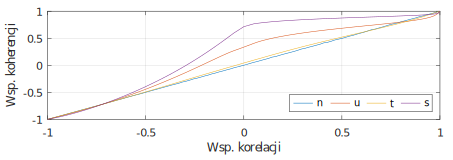
\includegraphics{obrazki/cohers}
\makecaption{fig:unc_cohers}{Zestawienie zależności wartości współczynników koherencji w funkcji współczynnika korelacji dla wybranych rodzajów rozkładu analizowanych sygnałów}
\end{center}
\end{figure}

Analizując przedstawione zależności zauważyć można, że sposób przedstawienia niedokładności wyniku pomiaru zależeć będzie w dużej mierze od potrzeb projektanta toru pomiarowego oraz od specyfiki zakłócających proces pomiaru błędów. Opis wykorzystujący wariancję błędów wydaje się bardziej przystępny, gdyż wariancja może być utożsamiana z mocą sygnału. Opis wykorzystujący niepewność rozszerzoną będzie jednak bardziej precyzyjny, natomiast wymaga większego zaangażowania w proces wyznaczania ostatecznej wartości tej niepewności. W odpowiednich okolicznościach, jeżeli spełnione są warunki związane z centralnym twierdzeniem granicznym, opis bazujący na wariancji błędu może być w łatwy sposób przeniesiony na opis związany z niepewnością rozszerzoną. Podczas wyznaczania wypadkowej wartości niepewności rozszerzonej stosować można metodę redukcyjnej arytmetyki interwałowej, opisaną szerzej w~\cite{jakubiec_reductive, jakubiec_arithmetic, jakubiec_redmono, batko_uncertainty}. Wyznaczone wartości niepewności rozszerzonej mogą w niewielkim stopniu odbiegać od wartości rzeczywistych, co opisano w~\cite{jakubiec_arithmetic, jakubiec_model}. Przyjmuje się jednak, że różnice nie przekraczające $5\%$ wartości prawdziwej są akceptowalne, przy czym bardziej korzystne są sytuacje gdzie błąd oszacowania cechuje się dodatnim znakiem -- tj. oszacowana wartość jest większa od rzeczywistej.

\section{Algorytm jako fragment toru pomiarowego}

Podczas opisu właściwości cyfrowej części toru pomiarowego przedstawiono przypadek, w którym analizowany obiekt przetwarzał kolejne próbki sygnału wejściowego na próbki sygnału wyjściowego zgodnie z odpowiadającą mu transmitancją i funkcją przetwarzania. Algorytmy stosowane w torach pomiarowych mogą generować wiele wielkości wyjściowych, pobierając przy tym w oknie pomiarowym określoną liczbę próbek wielkości wejściowych. W przypadku, gdy wyjście analizowanego obiektu stanowi $M$ próbek wielkości wyjściowych wyznaczanych na podstawie $N$ próbek wielkości wejściowych, a funkcja przetwarzania tego obiektu jest liniowa, działanie obiektu przedstawić można w ogólnej postaci jako~\cite{jakubiec_algorithms, jakubiec_single}:
\begin{equation}
\begin{bmatrix}
X \emb{0}   \\
X \emb{1}   \\
\vdots      \\
X \emb{M-1}
\end{bmatrix}
=
\begin{bmatrix}
a_{0, 0}   &   a_{0, 1} &   \cdots   &   a_{0, N-1}      \\
a_{1, 0}   &   \ddots   &            &   a_{1, N-1}      \\
\vdots     &            &   \ddots   &   \vdots          \\
a_{M-1, 0} &   \cdots   &   \cdots   &   a_{M-1, N-1}
\end{bmatrix}
\begin{bmatrix}
x \emb{0}   \\
x \emb{1}   \\
\vdots      \\
x \emb{N-1}
\end{bmatrix}
\label{eq:alg_out_mat},
\end{equation}
gdzie $a_{i,j}$ to kolejne współczynniki macierzy transformacji. Równanie~\eqref{eq:alg_out_mat} można przedstawić również w postaci iloczynu:
\begin{equation}
\mathbf{X} = \mathbf{A} \cdot \mathbf{x} \label{eq:alg_out_mul},
\end{equation}
gdzie $\mathbf{X}$ jest wektorem wielkości wyjściowych, $\mathbf{A}$ macierzą transformacji oraz $\mathbf{x}$ wektorem wielkości wejściowych~\cite{jakubiec_algorithms}. Wobec przedstawionych zależności, pojedynczą wielkość wyjściową algorytmu przedstawić można w postaci:
\begin{equation}
X \emb{i} = a_{i, 0} x \emb{0} + a_{i, 1} x \emb{1} + \hdots + a_{i, N-1} x \emb{N-1} \label{eq:alg_out_single}.
\end{equation}
Na podstawie przedstawionych zależności zauważyć można, że analizowany obiekt stanowi w zasadzie zbiór filtrów o skończonej odpowiedzi impulsowej \enquote{FIR}. Przedstawione metody analizy będą zatem przypominały metody analizy opisywanego typu filtru~\cite{mehrnia_fir}.

W praktyce wartości współczynników macierzy transformacji opisanej równaniem~\eqref{eq:alg_out_mat} mogą nie być znane przez projektanta toru pomiarowego. Ich znajomość jest jednak konieczna w celu przeprowadzenia analizy metrologicznej zastosowanego algorytmu. Najczęściej projektant toru pomiarowego stosuje gotowy algorytm, zaimplementowany np. w środowisku \enquote{GNU Octave} lub dostarczany mu jako zewnętrzną bibliotekę. W takim przypadku należy przeprowadzić proces identyfikacji wartości współczynników macierzy, który przedstawiony zostanie w dalszej części rozdziału. Innym przypadkiem jest sytuacja, w której z punktu widzenia analizy metrologicznej macierzowy opis algorytmu jest korzystny, a wartości współczynników mogą być wyznaczone za pomocą odpowiednich funkcjonałów. Ostatnim przypadkiem jest sytuacja, w której znana jest transmitancja $H(z)$ dla kolejnych wielkości wyjściowych. Wtedy wyznaczenie wartości współczynników macierzy transformacji odbywać się będzie poprzez przekształcenie tej transmitancji na postać zgodną z równaniem~\eqref{eq:alg_out_single}. Należy jednak zauważyć, że nie we wszystkich przypadkach przedstawione metody znajdują zastosowanie.

W przypadku, gdy dysponuje się gotową implementacją algorytmu, w celu identyfikacji współczynników macierzy transformacji należy podawać na wejście algorytmu wektor wielkości wejściowych, którego wszystkie elementy poza wybranym mają wartość zero. Wartość jednego elementu należy ustawić na jeden, a następnie za pomocą identyfikowanego algorytmu wyznaczyć należy wektor wielkości wyjściowych. Wyznaczony wektor stanowi kolumnę identyfikowanej macierzy transformacji, przy czym numer kolumny jest równy indeksowi elementu, który w wektorze wielkości wejściowych posiadał wartość jeden. W celu wyznaczenia wszystkich wartości macierzy transformacji należy powtórzyć powyższą czynność dla wektorów wartości wejściowych algorytmu zgodnie z zależnością~\cite{jakubiec_algorithms}:
\begin{equation}
x \emb{n} =
\begin{cases}
	1 & $gdy$~n = i \\
	0 & $gdy$~n \neq i
\end{cases}
\label{eq:wt_ident},
\end{equation}
dla $i$ w przedziale $<0;N-1>$, gdzie $i$ jest indeksem identyfikowanej kolumny macierzy transformacji. Niezależnie od struktury numerycznej analizowanego obiektu opisana metoda jest uniwersalna, przy czym wymaga ona, aby identyfikowany algorytm spełniał założenia przedstawione na początku podrozdziału.

Aby ustalić związek pomiędzy błędami wielkości wejściowych, a błędami wielkości wyjściowych analizowanego algorytmu należy przeanalizować proces wyznaczania wartości pojedynczej wielkości wyjściowej tego algorytmu. Wobec tego, jeżeli wielkości wejściowe algorytmu są obarczone błędami o charakterze addytywnym zgodnie z zależnością:
\begin{equation}
\tilde{x} \emb{i} = \dot{x} \emb{i} + e_{x,\Sigma} \emb{i} = \dot{x} \emb{i} + e_{x,s} \emb{i} + e_{x,d} \emb{i} + e_{x,r} \emb{i} \label{eq:alg_inputval},
\end{equation}
gdzie $e_{x,s}$ oznacza błąd statyczny, $e_{x,d}$ błąd dynamiczny oraz $e_{x,r}$ błąd losowy wielkości wejściowej, to istnieje możliwość osobnej analizy wyniku algorytmu dla idealnych wartości wielkości wejściowych oraz dla związanych z nimi błędów. Błąd wielkości wyjściowej przenoszony z wejścia na wyjście algorytmu można zatem opisać, zgodnie z równaniem~\eqref{eq:alg_out_single}, jako kombinację liniową współczynników transformacji algorytmu oraz błędów wielkości wejściowych:
\begin{equation}
e_{X,p} \emb{i} = a_{i, 0} e_{x,\Sigma} \emb{0} + a_{i, 1} e_{x,\Sigma} \emb{1} + \hdots + a_{i, N-1} e_{x,\Sigma} \emb{N-1} \label{eq:alg_outerr}.
\end{equation}

Dla błędów o charakterze statycznym, ze względu na fakt że realizacja tych błędów jest niezmienna w obrębie okna pomiarowego, równanie~\eqref{eq:alg_outerr} można uprościć i zapisać w postaci:
\begin{equation}
e_{X,s} \emb{i} = a_{i, 0} e_{x,s} + a_{i, 1} e_{x,s} + \hdots + a_{i, N-1} e_{x,s} = e_{x,s} \sum _{j = 0} ^{N-1} a_{i, j} \label{eq:alg_outerr_stat},
\end{equation}
gdzie $e_{x,s}$ jest błędem statycznym wielkości wejściowej, natomiast $e_{X,s}$ błędem statycznym wielkości wyjściowej algorytmu. Powtarzając pomiar wielokrotnie, dla różnych pozycji okna pomiarowego, realizacje błędu statycznego mogą przyjmować różne wartości. W takim przypadku wyjściowy błąd statyczny również można rozpatrywać w kategoriach probabilistycznych, a jego wariancję opisać można równaniem uwzględniającym wariancję wejściowego błędu statycznego:
\begin{equation}
\sigma_{X,s}^{2} \emb{i} = \sigma_{x,s}^{2} \left( a_{i, 0} + a_{i, 1} + \hdots + a_{i, N-1} \right)^{2} = \sigma_{x,s}^{2} \left( \sum _{j = 0} ^{N-1} a_{i, j} \right)^{2} \label{eq:alg_outvar_stat}.
\end{equation}
Należy zauważyć, że kształt rozkładu wyjściowego błędu statycznego będzie identyczny, jak kształt rozkładu statycznego błędu wejściowego.

Dla błędów o charakterze dynamicznym należy przeprowadzić analizę zgodnie z metodologią przedstawioną w poprzedniej części rozdziału, wykorzystując znajomość transmitancji $H(z)$ odpowiedniej dla analizowanej wielkości wyjściowej algorytmu. Identycznie, jak w przypadku równania~\eqref{eq:mid_disc_err_dyn_prop}, wyznaczyć należy wypadkowe amplitudy oraz przesunięcia w fazie kolejnych harmonicznych błędu dynamicznego, a następnie złożyć je zgodnie z zależnością~\eqref{eq:dyn_multi}. Transmitancja $H(z)$ dla $i$-tej wielkości wyjściowej może zostać wyznaczona na podstawie wartości współczynników $i$-tego wiersza macierzy transformacji algorytmu jako:
\begin{equation}
H_{i} \emb{z} = a_{i, 0} + a_{i, 1} z^{-1} + \hdots + a_{i, N-1} z^{-N+1} = \sum _{k = 0} ^{N-1} a_{i, k} z^{-k} \label{eq:alg_trans_single}.
\end{equation}
W omawianym przypadku przyjmuje się, że algorytm posiada idealną transmitancję, a ewentualne rozbieżności nie mają wpływu na widmo przenoszonego sygnału. Dodatkowe informacje związane z tym zagadnieniem zostaną przedstawione w dalszej części podrozdziału.

W przypadku błędów o charakterze losowym, wykonując algorytm wielokrotnie, uzyskać można zależność wiążącą wariancję błędu na wyjściu algorytmu z wariancją błędów wielkości wejściowych. Zakładając, że wszystkie wielkości wejściowe algorytmu pochodzą z tej samej cześć toru pomiarowego, a zatem ich parametry statystyczne są identyczne, oraz że kolejne błędy wielkości wejściowych nie są ze sobą skorelowane, zależność tą opisać można jako:
\begin{equation}
\sigma_{r}^{2} \emb{i} = a_{i, 0}^{2} \sigma_{x,r}^{2} + a_{i, 1}^{2} \sigma_{x,r}^{2} + \hdots + a_{i, N-1}^{2} \sigma_{x,r}^{2} = \sigma_{x,r}^{2} \sum _{j=0} ^{N-1} {a_{i, j}^{2}} \label{eq:alg_outvar_rand}.
\end{equation}

Poza przenoszeniem przez algorytm błędów zawartych w wielkościach wejściowych na jego wyjście, algorytm wprowadza do wielkości wyjściowych błędy własne. Błędy te wynikają niedokładności wyznaczenia współczynników algorytmu oraz z przeprowadzanych podczas obliczeń zaokrągleń. Ich wartości będą zatem uzależnione od wielu czynników, a ich analiza powinna odbywać się indywidualnie dla zaimplementowanego algorytmu. Zakładając, że wyznaczanie wartości $i$-tej wielkości wyjściowej algorytmu odbywać się będzie wielokrotnie, błędy własne opisywać można w kategorii probabilistycznej za pomocą związanej z nimi wariancji $\sigma_{X,z}^{2}(i)$. Ze względu na fakt, że liczba operacji mnożenia i dodawania, odpowiedzialnych za powstawanie omawianej grupy błędów będzie duża ($N$ mnożeń oraz $N$ dodawań) błąd ten będzie miał rozkład zbliżony do normalnego~\cite{jcgm_guide}. W przypadku, gdy na etapie identyfikacji wartości macierzy współczynników uzyskano wartości obarczone błędami, należy rozszerzyć analizę o przedstawienie konsekwencji tego zjawiska. W takim przypadku należy przeanalizować wprowadzany do wielkości wyjściowych statyczny błąd własny oraz wykonać analizę dla błędów własnych dynamicznych, analogicznie jak opisano równaniem~\eqref{eq:mid_disc_err_dyn_self}. Omawiany przypadek nie będzie rozpatrywany w pracy, ponieważ identyfikując wartości macierzy transformacji za pomocą przedstawionego algorytmu lub wyznaczając ich wartości przy użyciu odpowiednich funkcjonałów, wprowadzany błąd wynikać będzie głównie z zaokrągleń i będzie można analizować go równolegle z wprowadzanym losowym błędem $e_{X,z}$. Omawianą analizę przedstawia szczegółowo praca~\cite{jakubiec_system}.

Wobec powyższych założeń, w celu wyznaczenia wariancji $\sigma_{X,\Sigma}^{2}(i)$ wypadkowego błędu $e_{X,\Sigma}(i)$ dla $i$-tej wielkości wyjściowej analizowanego algorytmu należy wykorzystać zależność~\eqref{eq:var_matrix}, przy czym przyjmuje ona w tym przypadku postać:
\begin{equation}
\sigma_{X,\Sigma}^{2} \emb{i} =
\begin{bmatrix}
\sigma_{X,s} \emb{i} \\ \sigma_{X,d} \emb{i} \\ \sigma_{X,r} \emb{i} \\ \sigma_{X,z} \emb{i}
\end{bmatrix}^{T}
\begin{bmatrix}
1         & r_{d,s} & r_{r,s} & r_{z,s} \\
r_{s,d}   & 1       & r_{r,d} & r_{z,d} \\
r_{s,r}   & r_{d,r} & 1       & r_{z,r} \\
r_{s,z}   & r_{d,z} & r_{r,z} & 1
\end{bmatrix}
\begin{bmatrix}
\sigma_{X,s} \emb{i} \\ \sigma_{X,d} \emb{i} \\ \sigma_{X,r} \emb{i} \\ \sigma_{X,z} \emb{i}
\end{bmatrix}
\label{eq:alg_outvar_mat},
\end{equation}
gdzie $r_{i,j}$ stanowi współczynnik macierzy korelacji dla wybranych błędów cząstkowych analizowanego algorytmu. Wyznaczenie niepewności rozszerzonej może być przeprowadzone zgodnie z zależnością~\eqref{eq:unc_matrix}, przekształconą do postaci:
\begin{equation}
U_{X,\Sigma} \emb{i} = \sqrt{
\begin{bmatrix}
U_{X,s} \emb{i} \\ U_{X,d} \emb{i} \\ U_{X,r} \emb{i} \\ U_{X,z} \emb{i}
\end{bmatrix}^{T}
\begin{bmatrix}
1         & h_{d,s} & h_{r,s} & h_{z,s} \\
h_{s,d}   & 1       & h_{r,d} & h_{z,d} \\
h_{s,r}   & h_{d,r} & 1       & h_{z,r} \\
h_{s,z}   & h_{d,z} & h_{r,z} & 1
\end{bmatrix}
\begin{bmatrix}
U_{X,s} \emb{i} \\ U_{X,d} \emb{i} \\ U_{X,r} \emb{i} \\ U_{X,z} \emb{i}
\end{bmatrix}}
\label{eq:alg_outunc_mat},
\end{equation}
przy czym $h_{i,j}$ oznacza współczynnik koherencji wyznaczany zgodnie z zależnością~\eqref{eq:unc_coher}. Należy zauważyć, że równania~\eqref{eq:alg_outvar_mat} oraz~\eqref{eq:alg_outunc_mat} mogą zawierać więcej elementów składowych, niż wskazano. Dokładna postać przedstawionych równań zależeć będzie od budżetu niepewności wielkości wejściowych analizowanego algorytmu.

Na podstawie równań~\eqref{eq:alg_outvar_stat} oraz~\eqref{eq:alg_outvar_rand} wprowadzić można dodatkowe wielkości przedstawione następującymi zależnościami:
\begin{gather}
A_{i,s} = \sum _{j = 0} ^{N-1} a_{i, j} \label{eq:alg_trans_stat}, \\
A_{i,r} = \sqrt{\sum _{j = 0} ^{N-1} a_{i, j}^{2}} \label{eq:alg_trans_rand},
\end{gather}
gdzie $A_{i,s}$ jest współczynnikiem przenoszenia dla błędów statycznych, natomiast jest $A_{i,r}$ współczynnikiem przenoszenia dla błędów losowych $i$-tej wielkości wyjściowej analizowanego algorytmu. Wyznaczenie wartości opisanych współczynników umożliwi wyznaczenie wariancji kolejnych błędów losowych oraz statycznych, a dodatkowo będzie stanowiło informacje, w jaki sposób analizowany algorytm przenosi z wejścia na wyjście określony rodzaj błędu. Można zauważyć, że dla niskich wartości współczynnika przenoszenia (tj. $A_{i} < 1$) kolejne błędy wielkości wejściowych będą tłumione (wariancja błędu wielkości wyjściowej będzie mniejsza, niż wariancja błędów wielkości wejściowych). Odwrotna sytuacja będzie miała miejsce w przypadku dużych wartości współczynnika (tj. $A_{i} > 1$).

W przypadku analizy błędów dynamicznych, na podstawie równania~\eqref{eq:alg_trans_single} po podstawieniu $z = e^{j\omega}$, wyznaczyć można adekwatne dla równań~\eqref{eq:mid_disc_amp} oraz~\eqref{eq:mid_disc_phi} zależności opisujące wzmocnienie $K_{X,i}(\omega_{n})$ oraz przesunięcie w fazie $\varphi_{X,i}(\omega_{n})$ przetwarzanych harmonicznych sygnału w funkcji pulsacji znormalizowanej $\omega_{n}$ dla $i$-tej wielkości wyjściowej algorytmu w postaci:
\begin{gather}
G_{X,i} \emb{\omega_{n}} = \sum _{k = 0} ^{N-1} a_{i,k} e^{-j k \omega_{n}} \label{eq:alg_trans_norm}, \\
K_{X,i} \emb{\omega_{n}} = \left| G_{X,i} \emb{\omega_{n}} \right| = \sqrt{\left( \Re \left( G_{X,i} \emb{\omega_{n}} \right) \right)^{2} + \left( \Im \left( G_{X,i} \emb{\omega_{n}} \right) \right)^{2}} \label{eq:alg_trans_amp}, \\
\varphi_{X,i} \emb{\omega_{n}} = \arctan \left( \frac{\Im \left( G_{X,i} \emb{\omega_{n}} \right)}{\Re \left( G_{X,i} \emb{\omega_{n}} \right)} \right) \label{eq:alg_trans_phi},
\end{gather}
przy czym pulsacja znormalizowana, oznaczona symbolem $\omega_{n}$, odnosi się do pulsacji próbkowania i jest określona przez następującą zależność:
\begin{equation}
\omega_{n} = 2\pi \frac{\omega}{\omega_{s}} \label{eq:puls_norm},
\end{equation}
gdzie $\omega$ jest analizowaną pulsacją, natomiast $\omega_{s}$ pulsacją próbkowania równą $\frac{2 \pi}{T_{p}}$ dla okresu próbkowania $T_{p}$. Prawidłowa wartość pulsacji znormalizowanej mieści się zatem w zakresie $<0;\pi>$, co odpowiada zakresowi od zera do pulsacji Nyquista dla przyjętego okresu próbkowania.

\section{Podsumowanie przedstawionych zależności}

W poprzednich częściach rozdziału przedstawiono modele kolejnych fragmentów toru pomiarowego, które opisywały związki pomiędzy błędami na wejściu i wyjściu analizowanego obiektu, a także wskazywały rolę tego obiektu we wprowadzaniu do sygnału wyjściowego błędów własnych. Zaproponowany model wprowadzał podział na statyczne i dynamiczne właściwości obiektu, które opisywane były transmitancją i funkcją przetwarzania obiektu. Opisane zaproponowanym modelem fragmenty toru pomiarowego, które zostały ze sobą połączone kaskadowo oraz cechują się addytywną funkcją przetwarzania, opisać można modelem wypadkowym oraz z osobna analizować zawarte w nim błędy cząstkowe. Zaproponowana metoda wyznaczania niepewności wypadkowej bazuje na określeniu związków pomiędzy kolejnymi niepewnościami składowymi, a następnie wykorzystuje redukcyjną arytmetykę interwałową do wyznaczenia niepewności wypadkowej. Zaproponowany opis uwzględnia ewentualne korelacje pomiędzy kolejnymi grupami błędów, a w przypadku braku tych korelacji wymaga jedynie określenia związków pomiędzy kształtem rozkładu kolejnych składanych błędów~\cite{jakubiec_reductive, batko_uncertainty}.

Przedstawiony model oceny dokładności wyniku pomiaru zakłada, że obecne w sygnale pomiarowym błędy cechują się symetrycznymi rozkładami o zerowej wartości oczekiwanej. W przypadku, gdy wartość oczekiwana realizacji błędu jest niezerowa, błąd ten posiada składową systematyczną, którą należy skorygować w ostatecznym wyniku pomiaru. Jeżeli nie jest spełnione założenie odnośnie symetrii rozkładów składanych błędów, to do określenia rozkładu błędu wynikowego należy stosować metodę analityczną bazującą na wyznaczeniu splotu składanych funkcji gęstości prawdopodobieństwa lub wykorzystać metodę Monte-Carlo, która jest zwykle bardziej przystępna i optymalna ze względu na mniejszy stopień skomplikowania~\cite{janssen_montecarlo, roj_annuncertainty}.

Przeprowadzone rozważania nie poruszały problemu opóźnień w systemach pomiarowo-sterujących, a zatem nie brano w nich pod uwagę błędów związanych z opóźnieniami. Tematyka ta nie będzie poruszana w dalszych częściach pracy. Warto jednak zauważyć, że zaproponowany model błędu może być z łatwością dopasowany do możliwości analizy właściwości i wpływu tych błędów na niedokładność wielkości wyjściowych. Należy wtedy uwzględnić w modelu dodatkowy składnik błędu, który definiować można zgodnie z metodą zaproponowaną w~\cite{wymyslo_delay, jakubiec_system}. Z punktu widzenia zaproponowanego modelu, zjawisko to opisać można jako dodatkowe przesunięcie w fazie składowych przetwarzanego sygnału, będące iloczynem pulsacji analizowanej harmonicznej i wartości realizacji błędu opóźnienia.

\chapter{Algorytm transformacji falkowej}

Algorytm transformacji falkowej oznaczany skrótem \enquote{WT} (ang. \enquote{Wavelet Transform}) jest przekształceniem umożliwiającym analizę sygnału w dziedzinie skala-czas \cite{wallen_handbook}. Skala w przypadku algorytmu transformacji falkowej stanowi wybrany zakres częstotliwości składowych (harmonicznych) analizowanego sygnału. Jest to podobna cecha, jak w przypadku algorytmu \enquote{STFT} (ang. \enquote{Short-time Fourier transform}) \cite{durak_sftp}, będącego modyfikacją transformacji Fouriera. W ogólnej formie algorytm ciągłej transformacji falkowej (\enquote{CWT} -- ang. \enquote{Continous Wavelet Transform}) opisać można równaniem \cite{lord_guide, wallen_handbook}:
\begin{equation}
w_{a,b} = \frac{1}{\sqrt{a}} \int _{-\infty} ^{\infty} x \left( t \right) \psi \left( \frac{t-b}{a} \right) dt \label{eq:cwt},
\end{equation}
gdzie $w$ jest wyznaczonym współczynnikiem transformacji falkowej, $a$ parametrem skali, $b$ parametrem przesunięcia w czasie, natomiast $\psi$ równaniem falki-matki.

Parametr skali określa zakres częstotliwości -- im większa wartość tego parametru, tym falka staje się bardziej \enquote{rozciągnięta}, przez co odpowiada niższym częstotliwością sygnału ($a > 1$); w przypadku niskich wartości parametru skali ($a < 1$) falka staje się co raz bardziej \enquote{zwarta}, co odpowiada wyższym zakresom częstotliwości. Parametr przesunięcia w czasie określa okno pomiarowe dla wybranego współczynnika. Wybór równania falki-matki zależy od charakteru przetwarzanego sygnału oraz pożądanych właściwości falki. Literatura opisuje bardzo wiele różnych falek wraz z obszarami ich zastosowań \cite{wallen_handbook, akujuobi_applications}.

Główny podział falek pod katem ich właściwości obejmuje kilka najważniejszych cech charakterystycznych dla danej rodziny: ortogonalność, symetrię i biortogonalność. Ortogonalność oznacza, że dla wybranych parametrów skali i przesunięcia w czasie kolejne falki powstałe na bazie falki-matki będą wobec siebie ortogonalne. Jest to cecha w większości przypadków wymagana i pożądana. Symetria w przypadku falki-matki jest cenną cechą głównie w przypadku przetwarzania obrazów -- nie wszystkie rodziny falek posiadają tą cechę, stąd wiele prac skupiało się na \enquote{udoskonalaniu} istniejących rodzin pod katem wprowadzenia symetrii. Biortogonalność natomiast oznacza, że w celu rekonstrukcji sygnału należy zastosować odpowiednią dla użytej falki-matki powiązaną z nią falkę.

Ze względu na swoje właściwości, algorytmy transformacji falkowej są wykorzystywane w wielu dziedzinach \cite{akujuobi_applications}, przy czym w zależności od właściwości analizowanego sygnału stosuje się odpowiednią w danym przypadku falkę-matkę. W medycynie transformacja falkowa wykorzystywana jest między innymi do analizy sygnału EEG oraz EKG \cite{ocak_medicine}, a także wielu innych aplikacjach \cite{unser_medicine}. Transformacja falkowa znajduje również zastosowanie w przetwarzaniu obrazu oraz dźwięku \cite{kotteri_imagecomp}, głównie ze względu na możliwość zastosowania jej w algorytmach kompresji danych \cite{reddy_compression}. Ze względu na możliwości analizy sygnału zarówno w skali częstotliwości, jak i czasu, algorytmy transformacji falkowej znajdują swoje zastosowanie w analizie drgań sejsmicznych \cite{anping_seismic}. Analiza falkowa stosowana jest również w mechanice, gdzie istnieje możliwość oszacowania stanu zużycia elementów mechanicznych maszyny na podstawie wielkości wyjściowych algorytmu transformacji falkowej \cite{yan_mechanics}. Jednym z istotnych zastosowań jest także redukcja szumu w sygnale pomiarowym \cite{auth_denoise}, gdzie wykorzystywane są w dużej mierze falki podwójnej gęstości \enquote{dden} \cite{vimala_ddendenoise}. Mnogość zastosowań omawianych algorytmów jest zatem bardzo duża. Ze względu na fakt, że stanowią one istotną część toru pomiarowego, ich właściwości metrologiczne nie mogą być pomijane podczas analizy metrologicznej.

\section{Algorytm ciągłej transformacji falkowej}

Algorytm ciągłej transformacji falkowej może być stosowany w celu detekcji, czy i w jakim czasie widmo sygnału zawierało wybrane harmoniczne \cite{anping_seismic}. W tym przypadku istnieje możliwość wyznaczenia dowolnej liczby współczynników transformacji, gdzie ich liczba zależy od wymaganej rozdzielczości w skali czasu i częstotliwości \cite{wallen_handbook}. W przypadku tej wersji algorytmu rozdzielczość w dziedzinie czasu jest zwykle stała i nie zmienia się dla kolejnych skal częstotliwości. Rysunek \ref{fig:cobe_time} przedstawia przykładowy sygnał powiązany z przebiegiem trzęsienia ziemi w dziedzinie czasu, natomiast rysunek \ref{fig:cobe_cwt} przedstawia jego widmo uzyskane za pomocą algorytmu ciągłej transformacji falkowej. Na podstawie widma sygnału można określić w jakim czasie miało miejsce badane zjawisko, wiedząc jaka częstotliwość sygnału jest związana z tym zjawiskiem. Przerywana linia na wykresie widma oznacza obszar, dla którego wyniki nie są miarodajne -- w ich przypadku okno pomiarowe nie obejmowało wszystkich potrzebnych wielkości wejściowych.

\begin{figure}[htb!]
\begin{center}
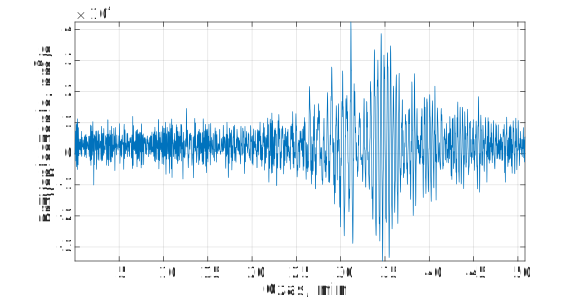
\includegraphics{obrazki/cobe_time}
\makecaption{fig:cobe_time}{Przebieg czasowy trzęsienia ziemi o sile 7.3 stopnia zarejestrowany w miejscowości Kobe w Japonii 17 stycznia 1995 roku}
\end{center}
\end{figure}

\begin{figure}[htb!]
\begin{center}
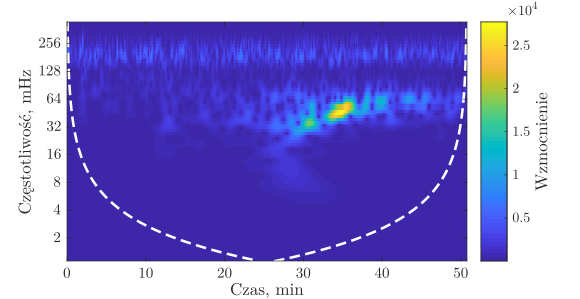
\includegraphics{obrazki/cobe_cwt}
\makecaption{fig:cobe_cwt}{Widmo czasowo-częstotliwościowe trzęsienia ziemi w Kobe z 17 stycznia 1995 roku przy zastosowaniu falki Morsa dla $\gamma = 3$}
\end{center}
\end{figure}

Algorytm ciągłej transformacji falkowej wymaga zastosowania opisanej ciągłym w dziedzinie czasu oraz częstotliwości równaniem falki-matki, natomiast nie wymaga aby określona była funkcja skalująca, której rola i znaczenie zostaną opisane w dalszej części pracy. Bazy stosowane w przypadku algorytmu ciągłej transformacji falkowej mogą być opisane zarówno w dziedzinie liczb rzeczywistych, jak i zespolonych. Ze względu na możliwość stosowania dowolnych wartości parametru skali i czasu, kolejne pochodne falki-matki nie są wobec siebie ortogonalne, co w praktyce oznacza że wyznaczane są w tym przypadku nadmiarowe współczynniki transformacji.

\section{Algorytm dyskretnej transformacji falkowej}

W praktyce wyznaczenie wszystkich współczynników algorytmu ciągłej transformacji falkowej jest niemożliwe. Wprowadzając ograniczenie możliwych wartości parametrów skali i czasu użytych w równaniu \eqref{eq:cwt}, w którym $a = 2^k$, $b = n2^k$ oraz $k, n \in \mathbb{N}$, uzyskuje się zależność opisującą algorytm dyskretnej transformacji falkowej (\enquote{DWT} -- ang. \enquote{Discrete Wavelet Transform}) \cite{wallen_handbook}. Termin \enquote{dyskretna} oznacza zatem ograniczony (dyskretny) zbiór możliwych wartości skali i przesunięcia w czasie.

Modyfikacja fragmentu równania \eqref{eq:cwt} wprowadzająca opisywane założenie dyskretyzacji parametrów skali i czasu oraz założenie początkowych wartości parametrów skali i czasu, gdzie $a_{0} = 2$ oraz $b_{0} = 1$, pozwala uzyskać zależność opisującą kolejne falki stworzone na bazie falki-matki dla dyskretnych wartości parametru numeru skali i przesunięcia w czasie:
\begin{equation}
\psi_{m,n} \left( t \right) = \frac{1}{\sqrt{2^{m}}} \psi \left( \frac{t-2n^{m}}{2^{m}} \right) \label{eq:dwt_wavelet},
\end{equation}
gdzie $m$ jest numerem skali, a $n$ numerem przesunięcia w czasie (numerem okna pomiarowego). Tak opisana falka jest zwykle ortogonalna oraz musi posiadać znormalizowaną energię, a zatem zapisać można:
\begin{equation}
\int _{-\infty} ^{\infty} \psi_{m,n} \left( t \right) \psi_{m',n'} dt =
\begin{cases}
	1 & $d $ m = m' $ oraz $ n = n' \\
	0 & $w pozostałych przypadkach$
\end{cases}
\label{eq:dwt_orthogonal}.
\end{equation}
W praktyce oznacza to, że nie ma możliwości opisu dowolnej stworzonej na podstawie równania \eqref{eq:dwt} falki pochodnej za pomocą podobnej falki o innym numerze skali lub czasu.

Podstawiając falkę opisaną równaniem \eqref{eq:dwt_wavelet} do równania \eqref{eq:cwt} otrzymuje się zależność opisującą dyskretną transformację falkową:
\begin{equation}
w_{m,n} = \frac{1}{\sqrt{2^{m}}} \int _{-\infty} ^{\infty} x \left( t \right) \psi \left( \frac{t-2n^{m}}{2^{m}} \right) dt \label{eq:dwt}.
\end{equation}
Cechą algorytmu dyskretnej transformacji falkowej jest dynamiczna zależność rozdzielczości dziedziny czasu w funkcji skali. Dla niskich wartości parametru skali (wysokich częstotliwości sygnału) rozdzielczość w dziedzinie czasu jest większa w porównaniu z rozdzielczością dla skali wyższych (niższych zakresów częstotliwości). Jako, że sygnał o wyższej częstotliwości zmienia się bardziej dynamicznie, niż w przypadku sygnału o niższej częstotliwości, takie podejście jest bardzo korzystne. Umożliwia ono redukcję liczby współczynników transformacji (wielkości wyjściowych algorytmu), przy jednoczesnym zachowaniu optymalnej rozdzielczości w dziedzinie czasu oraz zapewnieniu możliwości rekonstrukcji oryginalnego przebiegu sygnału na podstawie uzyskanych współczynników transformacji.

Ze względu na fakt, że falka-matka dla zadanej skali stanowi filtr pasmowo-przepustowy, przy czym zwiększanie skali powoduje przesunięcie charakterystyki filtru w kierunku niższych częstotliwości, w celu wyodrębnienia wszystkich częstotliwości z przetwarzanego sygnału należy wyznaczyć wartości współczynników transformacji dla nieskończonej liczby skal -- w innym wypadku wszystkie niskie zakresy częstotliwości nie zostaną przetworzone. Naturalnie nie jest to w praktyce możliwe. Aby rozwiązać problem analizy niskich częstotliwości przetwarzanego sygnału, stosuje się tzw. \enquote{funkcję skalującą} nazywaną również \enquote{falką-ojcem}. Funkcja ta, w przeciwieństwie do falki-matki, stanowi filtr dolno-przepustowy i zastępuje określony przedział niskich skal falki-matki -- w ten sposób eliminuje się potrzebę wyznaczania nieskończonej liczby współczynników transformacji przy jednoczesnej możliwości przetworzenia całego widma sygnału. Funkcja skalująca jest ściśle powiązana z falką-matką i jest oznaczana w literaturze jako $\phi(t)$ \cite{wallen_handbook}. Można w tym miejscu zauważyć, że aby dana rodzina falek mogła zostać wykorzystana przez algorytm dyskretnej transformacji falkowej, musi być dla niej określona odpowiednia funkcja skalująca.

Stosując podobne założenia, jak w równaniu \eqref{eq:dwt_wavelet}, otrzymuje się równanie funkcji skalującej dla dyskretnej wartości numeru skali i przesunięcia w czasie:
\begin{equation}
\phi_{m,n} \left( t \right) = \frac{1}{\sqrt{2^{m}}} \phi \left( \frac{t-2n^{m}}{2^{m}} \right) dt \label{eq:dwt_scalefun},
\end{equation}
Przy czym funkcję skalującą dla $m = n = 0$ nazywa się w literaturze \enquote{falką-ojcem} \cite{akujuobi_applications}. Właściwością funkcji skalującej jest spełnianie przez nią założenia odnośnie ograniczonej mocy, które jest opisane w postaci:
\begin{equation}
\int _{-\infty} ^{\infty} \phi_{0,0} \left( t \right) dt = 1 \label{eq:dwt_fatherwav},
\end{equation}
a także ortogonalność względem samej siebie dla dowolnych różnych wartości parametru numeru przesunięcia w czasie. Warto zaznaczyć, że w przypadku zmiany parametru numeru skali kolejne wersje funkcji skalującej nie są wobec siebie ortogonalne. W praktyce jednak nie ma to znaczenia, ponieważ współczynniki transformacji zależne od funkcji skalującej wyznacza się tylko dla jednej wartości parametru numeru skali oraz dla wszystkich dostępnych wartości parametru numeru przesunięcia w czasie. Opisywane zależności będą związane aproksymacją przetwarzanego sygnału.

Omawianą funkcję skalującą można przedstawić również w postaci sumy iloczynów współczynników skalowania oraz wartości przeskalowanej i przesuniętej w czasie funkcji skalującej, co opisuje następującą zależność:
\begin{equation}
\phi \left( t \right) = \sum _{k} ^{N_k-1} c_{k} \phi \left( 2t - k \right) \label{eq:dwt_scalefunrek},
\end{equation}
gdzie $k$ jest dowolną liczbą całkowitą powiązaną ze współczynnikiem skalowania $c_k$. Dodatkowo wszystkie współczynniki $c_k$ muszą spełniać założenia:
\begin{equation}
\sum _{k} ^{N_k-1} c_{k} = 2 \label{eq:dwt_scalefunsum}.
\end{equation}
Należy również zaznaczyć, że w celu zachowania warunku wzajemnej ortogonalności opisywanej rodziny falek, spełnione musi zostać dodatkowe założenie odnośnie wzajemnej relacji pomiędzy kolejnymi wartościami współczynników skalowania, w którym przyjmuje się że:
\begin{equation}
\sum _{k} ^{N_k-1} c_{k} c_{k+2k'} =
\begin{cases}
	2 & $gdy$ ~ k' = 0 \\
	0 & $w pozostałych przypadkach$
\end{cases}
\label{eq:dwt_scalemulort}.
\end{equation}
Powyższe założenia zapewniają ortogonalność stworzonych falek w stosunku do funkcji skalującej oraz brak nadmiarowych współczynników wyjściowych algorytmu dyskretnej transformacji falkowej. Tworzone na opisanych zasadach falki posiadają skończoną liczbę niezerowych współczynników skalujących $c_k$, przy czym rząd falki $N_r$ określa liczbę tych współczynników równą $N_{k} = 2 N_r$. Manipulując odpowiednio znakiem i kolejnością współczynników skalujących istnieje możliwość opisu falki-matki za pomocą równania \cite{wallen_handbook}:
\begin{equation}
\psi \left( t \right) = \sum _{k} ^{N_k-1} \left( -1 \right) ^{k} c_{N_k-k-1} \phi \left( 2t - k \right) \label{eq:dwt_waveletfunrek}.
\end{equation}
Ostatecznie przedstawić można rekursywne zależności opisujące funkcję skalującą i funkcję falki dla dowolnego numeru skali i numeru przesunięcia czasowego za pomocą równań:
\begin{gather}
\psi_{m+1,n} \left( t \right) = \frac{1}{\sqrt{2}} \sum _{k} ^{N_k-1} c_{k} \psi_{m,2n+k} \left( t \right) \label{eq:dwt_fatherrek}, \\
\phi_{m+1,n} \left( t \right) = \frac{1}{\sqrt{2}} \sum _{k} ^{N_k-1} b_{k} \psi_{m,2n+k} \left( t \right) \label{eq:dwt_matherrek},
\end{gather}
przy czym parametr $b_{k}$ przedstawić można jako rekombinacje współczynników skalujących:
\begin{equation}
b_{k} = \left( -1 \right) ^{k} c_{N_k-k-1} \label{eq:dwt_bk}.
\end{equation}

Dekompozycja sygnału w przypadku algorytmu dyskretnej transformacji falkowej odbywa się w ten sposób, że sygnał wejściowy podawany jest na wejścia pary filtrów -- górno i dolno przepustowego. Wyjście filtru dolno przepustowego stanowi aproksymacje sygnału, natomiast wyjście filtru górno przepustowego stanowią detale sygnału. Ze względu na fakt, że opisywana operacja dostarcza dwa razy więcej próbek wyjściowych, niż zawierał oryginalny sygnał, co druga próbka wyjściowa jest usuwana w procesie decymacji. Opisywane działanie rozdziela widmo sygnału na dwie części: detale sygnału związane z wysokimi częstotliwościami oraz aproksymacje sygnału powiązaną z niskimi zakresami częstotliwości. Filtr dolno-przepustowy odpowiada charakterystyce funkcji skalującej, natomiast filtr górno-przepustowy charakterystyce falki-matki. Filtr górno-przepustowy jest więc faktycznie filtrem pasmowo-rzepustowym, natomiast ze względu na wartość parametru skali jego częstotliwość środkowa odpowiada częstotliwości Nyquista dla przetwarzanego sygnału -- stąd też można w uproszczeniu nazwać go filtrem górno-przepustowym. Proces dekompozycji sygnału może zostać powtórzony dla aproksymacji sygnału wielokrotnie, zapewniając większą rozdzielczość w dziedzinie częstotliwości kosztem mniejszej rozdzielczości w dziedzinie czasu. Przebieg procesu dekompozycji sygnału dla trzech iteracji opisywanego procesu przedstawiono na rysunku \ref{fig:dwt_decomposition}.

W celu rekonstrukcji sygnału należy zastosować odpowiedni bank filtrów, który w parze z bankiem filtrów wejściowych stanowi system zwany kwadraturowymi filtrami lustrzanymi \cite{johnston_filter}. Na wejście opisywanego filtru podać należy współczynniki uzyskane wcześniej na drodze dekompozycji sygnału wykonanej za pomocą lustrzanego filtru. Przebieg procesu rekonstrukcji sygnału dla trzech iteracji opisywanego procesu przedstawiono na rysunku \ref{fig:dwt_reconstruction}.

Na rysunkach \ref{fig:dwt_decomposition} oraz \ref{fig:dwt_reconstruction} \enquote{strzałką w górę} oznaczono uzupełnianie brakujących wielkości wejściowych współczynnikami o wartości zero. Działanie to wynika z faktu, że liczba wielkości wejściowych jest mniejsza, niż wymagana do wyznaczenia. \enquote{Strzałką w dół} oznaczono natomiast proces decymacji, czyli odrzucania co drugiej wielkości wyjściowej. Pominięcie tego procesu spowodowałoby, że wielkości wyjściowych byłoby dwa razy więcej, niż jest to wymagane w celu rekonstrukcji sygnału. Symbol $S$ na rysunkach oznacza wielkości wyjściowe związane z detalami sygnału, a symbol $T$ wielkości wyjściowe związane z aproksymacją sygnału. Indeks dolny jest związany z numerem iteracji procesu dekompozycji. Opisywany algorytm w literaturze nosi nazwę \enquote{Algorytm Malata} lub \enquote{FWT} (ang. \enquote{Fast Wavelet Transform}) i został opracowany w 1988 roku przez Stéphane Mallata \cite{lujian_mallat}.

\begin{figure}[htb!]
\begin{center}
\includegraphics{obrazki/dwt_dekompozycja}
\makecaption{fig:dwt_decomposition}{Proces dekompozycji sygnału za pomocą algorytmu Mallata}
\end{center}
\end{figure}

\begin{figure}[htb!]
\begin{center}
\includegraphics{obrazki/dwt_rekonstrukcja}
\makecaption{fig:dwt_reconstruction}{Proces rekonstrukcji sygnału za pomocą algorytmu Mallata}
\end{center}
\end{figure}

Pominiecie procesu decymacji powoduje powstanie nadmiarowych wielkości wyjściowych algorytmu i jest praktykowane w przypadku algorytmu \enquote{UWT} (ang. \enquote{Undecimated Wavelet Transform}). W przypadku tej odmiany algorytmu transformacji falkowej, dla każdego poziomu dekompozycji wyznaczanych jest tyle wielkości wyjściowych, ile wielkości wejściowych zawierał przetwarzany sygnał. Praktyczna realizacja algorytmu niedecymowanej transformacji falkowej jest bardzo podobna do realizacji algorytmu ciągłej transformacji falkowej. Algorytmy dyskretnej transformacji falkowej w klasycznym przypadku posiadają identyczną liczbę próbek wielkości wyjściowych i wejściowych. Istnieją jednak przypadki, w których liczba wielkości wyjściowych jest większa od liczby wielkości wyjściowych -- np. w przypadku falek podwójnej gęstości \cite{selenick_ddenusage}. Różnica ta wynika z modyfikacji procesu dekompozycji sygnału w przypadku falek podwójnej gęstości.

Zgodnie z przedstawionymi wcześniej zależnościami, omawiany proces dekompozycji sygnału można opisać również rekurencyjnie za pomocą równań \cite{wallen_handbook}:
\begin{gather}
S_{m+1,n} = \frac{1}{\sqrt{2}} \sum _{k} ^{N_k-1} c_{k} S_{m,2n+k} \label{eq:dwt_aproxrek}, \\
T_{m+1,n} = \frac{1}{\sqrt{2}} \sum _{k} ^{N_k-1} b_{k} S_{m,2n+k} \label{eq:dwt_detailrek},
\end{gather}
natomiast proces rekonstrukcji sygnału opisać można za pomocą równania:
\begin{equation}
S_{m-1,n} = \frac{1}{\sqrt{2}} \left( \sum _{k} ^{N_k-1} c_{n-2k} S_{m,k} + \sum _{k} ^{N_k-1} b_{n-2k} T_{m,k} \right) \label{eq:dwt_reconrek},
\end{equation}
gdzie $S_{0,i}$ jest $i$-tą próbką przetwarzanego sygnału, $S_{m+1,n}$ aproksymacjami, a $T_{m+1,n}$ detalami sygnału dla zadanego numeru skali i przesunięcia w czasie. Współczynniki $c_i$ oraz $b_i$ są niezerowe tylko dla $i$ należących do przedziału $<0;N_k-1>$ -- poza tym przedziałem są one równe zero.

Wartości i liczba współczynników $c$ oraz $b$ zależy od zastosowanej rodziny falek i jej rzędu. W przypadku, gdy w wektorze wielkości wejściowych nie istnieje element o zadanym indeksie (tj. zachodzi $S_{m,i}$ lub $T_{m,i}$ dla $i \ge N$) należy przyjąć w obliczeniach wartość dla indeksu $i' = i \text{ mod } N$ gdzie \enquote{mod} jest resztą z dzielenia wyrazu po lewej stronie operatora przez wyraz z prawej strony operatora. W ten sam sposób postępować należy w przypadku procesu rekonstrukcji sygnału.

Ze względu na fakt, że ciągła transformacja falkowa jest w praktyce niemożliwa w realizacji, natomiast proces decymacji nie jest zwykle pomijany ze względu na brak potrzeby wyznaczania nadmiarowej liczby współczynników, dalsza część pracy poświęcona będzie algorytmowi dyskretnej transformacji falkowej. Przedstawiany w pracy sposób analizy właściwości metrologicznych będzie jednak jednolity dla rzeczywistych implementacji omawianych algorytmów.

\section{Bank filtrów algorytmu}

Zależnie od wymaganych kryteriów podczas stosowania algorytmów transformacji falkowej wybiera się odpowiednią do analizowanego sygnału falkę-matkę. Wybór falki-matki ma ogromny wpływ na proces dekompozycji sygnału, ponieważ to właśnie od niej zależą parametry banku filtrów, na którego wejście podawany jest przetwarzany przez algorytm sygnał. W przypadku algorytmów ciągłej transformacji falkowej istnieje możliwość zastosowania dowolnie dużej liczby kombinacji wartości parametru skali i przesunięcia w czasie, przez co dekompozycja sygnału jest bardziej dokładna.

Na rysunkach \ref{fig:demo_db}, \ref{fig:demo_spline} oraz \ref{fig:demo_dden} zaprezentowano przykładowe banki filtrów, gdzie na osi poziomej przedstawiono częstotliwość znormalizowaną do połowy częstotliwości próbkowania (częstotliwości Nyquista), a na osi pionowej znormalizowane do jedności wzmocnienie. Wzmocnienie zostało znormalizowane z osobna dla każdego poziomu dekompozycji w celu uczytelnienia wykresów i możliwości ich łatwiejszego porównywania. Kolorem niebieskim oznaczono na rysunkach charakterystyki filtru dolno-przepustowego powstałego na bazie funkcji skalującej. Pozostałe filtry powstały na bazie odpowiednio przeskalowanej falki-matki. Należy zauważyć, że w przypadku dyskretnej wersji algorytmu transformacji falkowej, w praktyce liczba etapów procesu dekompozycji jest ograniczona -- wraz ze zwiększaniem tej liczby maleje rozdzielczość w skali czasu dla aproksymacji sygnału, aż do chwili gdy aproksymacje sygnału stanowi jedna wielkość wyjściowa \cite{wallen_handbook}.

\begin{figure}[htb!]
\begin{center}
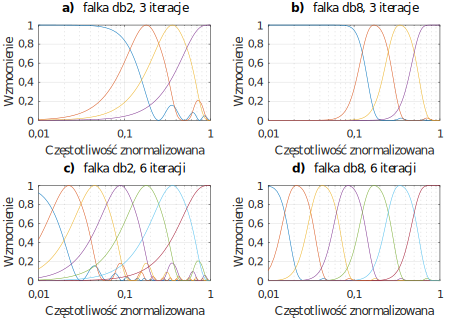
\includegraphics{obrazki/bank_db_demo}
\makecaption{fig:demo_db}{Banki filtrów dla falki \enquote{Daubechies}}
\end{center}
\end{figure}

Na podstawie wykresu zauważyć można, że dla kolejnych parametrów skali pasmo przenoszenia filtru jest o połowę mniejsze w stosunku do pasma przenoszenia filtru poprzedniej skali. Zgodnie z przedstawionymi charakterystykami, kolejne etapy dekompozycji sygnału przenoszą zatem fragment widma analizowanego sygnału zgodnie z charakterystyką zastosowanej falki-matki. Zależnie od właściwości falki-matki zbudowane na jej podstawie filtry mogą być mniej lub bardziej selektywne (wykazywać inną stromość charakterystyki filtru), czy też wykazywać cechy filtrów grzebieniowych (mogą przenosić kilka zakresów częstotliwości). Im bardziej skomplikowany będzie kształt falki i wyższy będzie jej rząd, tym zwykle bardziej selektywny będzie filtr stworzony na jej bazie. Wzrost liczby iteracji dekompozycji sygnału wprowadza kolejne filtry o węższym niż dla mniejszej liczby iteracji paśmie przenoszenia. Z analizy przedstawionych rysunków wynika, że w przypadku wszystkich przedstawionych rodzin falek, wzrost rzędu falki powoduje wzrost selektywności kolejnych filtrów. Część z przedstawionych falek zapewnia filtry podobne do filtrów grzebieniowych -- pasmo przenoszenia tych filtrów składa się z kilku przedziałów częstotliwości.

\begin{figure}[htb!]
\begin{center}
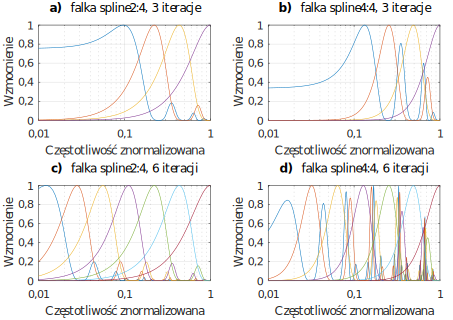
\includegraphics{obrazki/bank_spline_demo}
\makecaption{fig:demo_spline}{Banki filtrów dla falki \enquote{Spline}}
\end{center}
\end{figure}

\begin{figure}[htb!]
\begin{center}
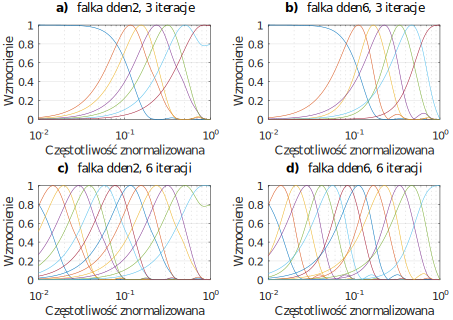
\includegraphics{obrazki/bank_dden_demo}
\makecaption{fig:demo_dden}{Banki filtrów dla falki \enquote{podwójnej gęstości}}
\end{center}
\end{figure}

Przedstawiona na osi pionowej maksymalna wartość wzmocnienia w funkcji częstotliwości sygnału może być w rzeczywistości większa od jedności. W praktyce każdy z fragmentów banku filtrów traktować można jako pasmowo-przepustowy filtr i opisywać za pomocą modelu filtru o skończonej odpowiedzi impulsowej (\enquote{FIR}). Z punktu widzenia pojedynczej wielkości wyjściowej, algorytm transformacji falkowej może być zatem rozumiany jako odpowiednio zaprojektowany filtr, który z sygnału wejściowego przenosi na wyjście wybrane harmoniczne sygnału wejściowego z odpowiednim wzmocnieniem i przesunięciem fazowym.

Przedstawione cechy banku filtrów będą bardzo istotne w dalszym etapie pracy w szczególności do określania, w jaki sposób algorytm przenosi błędy opisane w pracy jako dynamiczne. Należy zauważyć, że skoro kolejne filtry w banku odpowiadają kolejnym etapom dekompozycji sygnału, to w większości przypadków właściwości metrologiczne będą jednakowe dla wszystkich wielkości wyjściowych powiązanych z identycznym etapem dekompozycji sygnału.

W pewnych przypadkach wypadkowe właściwości toru pomiarowego mogą ulec zmianie, jeżeli wprowadzona zostanie dodatkowa modyfikacja wielkości wejściowych algorytmu transformacji falkowej (np. wprowadzone zostanie okno pomiarowe lub dodatkowy algorytm filtru). Należy w takim przypadku analizować właściwości metrologiczne każdej wielkości wyjściowej z osobna, a nie jak w klasycznym przypadku analizować je dla danego etapu dekompozycji. Taką modyfikację można również rozpatrywać w sposób identyczny, jak zmianę parametrów banku filtrów.

\section{Macierzowa postać algorytmu}

Ze względu na bardzo dużą liczbę opisanych w literaturze falek \cite{akujuobi_applications}, ich unikatowe właściwości oraz możliwość zmiany parametrów procesu dekompozycji sygnału, metody analityczne określenia właściwości metrologicznych dla wybranej kombinacji parametrów okazują się czasochłonne i niepraktyczne \cite{yan_uncertainty, wilczok_uncertainty, peretto_uncertainty, sarrafi_uncertainty}. Część opisywanych w literaturze falek obejmuje falki: \enquote{Daubechies} \cite{vonesch_dbbasics}, \enquote{Haara} \cite{stankovic_haar}, \enquote{Coiflet} \cite{wei_coiflet}, \enquote{Biortogonalne} \cite{sweldens_bior}, \enquote{Morleta} \cite{cohen_morlet}, \enquote{Meksykańskiej czapki} \cite{singh_mexican}, \enquote{Spline} \cite{averbuch_spline, wang_splinebasics}. Każdą falkę oraz przypisaną do niej funkcję skalującą opisują odpowiednie równania, przy czym nie zawsze są one zadane w postaci jawnej -- w wielu przypadkach rodzina falek opisana jest przez zbiór zależności określających wymagane przez nią założenia, co jeszcze bardziej komplikuje proces analizy tych algorytmów \cite{rowe_dbmath}.

Podczas projektowania toru pomiarowego często istnieje potrzeba zmiany parametrów algorytmu transformacji falkowej, co pociąga za sobą konieczność przeprowadzenia powtórnej analizy jego właściwości metrologicznych. Wszystkie te czynniki sprawiają, że analiza ta jest najczęściej pomijana w pracach opisujących aplikacje omawianych algorytmów. Z opisywanych właściwości algorytmów transformacji falkowej wynika potrzeba przedstawienia uniwersalnej metody umożliwiającej analizę właściwości metrologicznych tych algorytmów. Metoda ta musi być przystępna w aplikacji oraz musi zakładać, że projektant toru pomiarowego nie jest ekspertem w dziedzinie transformacji falkowej, a jedynie użytkownikiem tej transformacji. Co więcej, ewentualna zmiana parametrów zastosowanego algorytmu nie może być kłopotliwa z punktu widzenia określenia nowych właściwości metrologicznych analizowanego algorytmu.

Problem skomplikowanej analizy algorytmów transformacji falkowej, podobnie jak w przypadku innych algorytmów przetwarzających ciągi danych, uprościć można przedstawiając analizowany algorytm w postaci macierzowej. Wektor wielkości wyjściowych algorytmu jest wtedy równy iloczynowi macierzy transformacji i wektora wielkości wejściowych zgodnie z równaniem \eqref{eq:alg_out_mat}. Przedstawienie algorytmu transformacji falkowej w formie macierzowej umożliwi stworzenie jednolitego i uniwersalnego opisu działania tego algorytmu oraz w znaczącym stopniu ułatwi jego analizę w kolejnych rozdziałach pracy. Zwykle projektant toru pomiarowego nie jest ekspertem w dziedzinie falek -- jest on ekspertem w dziedzinie analizowanego zjawiska, a transformacja falkowa jest dla niego jedynie narzędziem, umożliwiającym jego analizę. Stąd w większości przypadków osoba ta stosuje gotowe biblioteki, zaimplementowane np. dla środowisk \enquote{Matlab}, \enquote{GNU Octave} czy \enquote{PyWavelets} \cite{lee_pywavelets, misiti_matlabwav}.

W celu identyfikacji wartości współczynników macierzy transformacji należy zastosować metodę opisaną w poprzednim rozdziale pracy lub wyznaczyć go analitycznie, jak zostanie to przedstawione w dalszej cześć rozdziału. Opisany wcześniej algorytm identyfikacji macierzy transformacji może być z łatwością zaimplementowany w środowiskach, które implementują algorytmy transformacji falkowej, przez co projektant toru pomiarowego z łatwością jest w stanie go zastosować. Ewentualna zmiana parametrów algorytmu transformacji falkowej (zmiana liczby wielkości wejściowych, liczby iteracji procesu dekompozycji, czy wybór innej falki-matki) skutkować będzie jedynie koniecznością ponownej identyfikacji wartości współczynników macierzy transformacji. W odróżnieniu od metod analitycznych nie zachodzi tutaj potrzeba stosowania skomplikowanych funkcjonałów w celu analizy zastosowanego algorytmu.

Poza opisanym algorytmem identyfikacji współczynników macierzy transformacji, bazującym na gotowej implementacji omawianego algorytmu, istnieje możliwość ich wyznaczenia przy użyciu zależności przedstawionych we wcześniejszej części rozdziału opisującej właściwości algorytmu dyskretnej transformacji falkowej. Proces ten jest jednak skomplikowany i uzależniony od założeń związanych z opisem zastosowanej falki-matki i jej funkcji skalującej. Poniżej zostanie przedstawiony przykład wyznaczania wartości macierzy transformacji w przypadku zastosowania falki \enquote{db2} dla dwóch iteracji procesu dekompozycji sygnału oraz ośmiu próbek wejściowych sygnału. Macierz transformacji będzie miała zatem wymiary ośmiu wierszy i ośmiu kolumn, natomiast wektor próbek wejściowych oraz wektor próbek wyjściowych będą zawierały po osiem elementów.

Rodzina falek \enquote{Daubechies} (w skrócie \enquote{db}) została opisana przez Ingrid Daubechies \cite{vonesch_dbbasics}, cechuje się ortogonalnością, natomiast nie wykazuje cech symetrii. Poza założeniami opisanymi w poprzednim podrozdziale rodzina ta spełnia dodatkowe założenie odnośnie relacji pomiędzy kolejnymi współczynnikami skalującymi:
\begin{equation}
\sum _{k} ^{N_k-1} \left( -1 \right)^{k} c_{k} k^{m} = 0 \label{eq:db_musthave},
\end{equation}
gdzie $m$ jest liczbą całkowitą z przedziału $<0;\frac{N_{k}}{2}-1>$.

W przypadku falek \enquote{db} oraz ich pochodnych, rząd falki wynosi $\frac{N_{k}}{2}$. Falka \enquote{db2}, będąca falką drugiego rzędu, posiada cztery niezerowe współczynniki skalujące. W literaturze spotkać się można również z oznaczeniem \enquote{D4} dla omawianej falki, gdzie zamiast rzędu falki wskazana jest liczba niezerowych współczynników skalujących. Falka \enquote{Daubechies} rzędu pierwszego jest opisana identycznymi zależnościami, jak falka Hara. Z falek \enquote{Daubechies} wywodzą się kolejne rodziny: \enquote{Symleth} oraz \enquote{Coiflet}, które uzupełniają ją o kolejne cechy -- w szczególności symetrię, istotną podczas przetwarzania i analizy obrazów.

Jako, że falka \enquote{db2} posiada cztery niezerowe współczynniki skalujące oznaczone jako $c_0, c_1, c_2, c_3$, to zgodnie z równaniem \eqref{eq:dwt_scalefunrek} oraz równaniem \eqref{eq:dwt_waveletfunrek}, zapisać można równanie falki-matki i funkcji skalującej w postaci:
\begin{gather}
\phi \left( t \right) = c_{0} \phi \left( 2t \right) + c_{1} \phi \left( 2t - 1 \right) + c_{2} \phi \left( 2t - 2 \right) + c_{3} \phi \left( 2t - 3 \right) \label{eq:db2_scalefunrek}, \\
\psi \left( t \right) = c_{3} \phi \left( 2t \right) - c_{2} \phi \left( 2t - 1 \right) + c_{1} \phi \left( 2t - 2 \right) - c_{0} \phi \left( 2t - 3 \right) \label{eq:db2_waveletfunrek}.
\end{gather}

Uwzględniając założenia przedstawione w poprzedniej części rozdziału oraz te wskazane powyżej, zapisać można układ równań wiążący wszystkie przedstawione zależności w postaci:
\begin{equation}
\begin{cases}
	c_{0} + c_{1} + c_{2} + c_{3} = 2                 & $na podstawie właściwości \eqref{eq:dwt_scalefunsum}$ \\
	c_{0}^{2} + c_{1}^{2} + c_{2}^{2} + c_{3}^{2} = 2 & $na podstawie właściwości \eqref{eq:dwt_scalemulort}$ \\
	c_{0} - c_{1} + c_{2} - c_{3} = 0                 & $na podstawie \eqref{eq:db_musthave} dla $ m = 0 \\
	- 1 c_{1} + 2 c_{2} - 3 c_{3} = 0                 & $na podstawie \eqref{eq:db_musthave} dla $ m = 1
\end{cases}
\label{eq:db2_system},
\end{equation}
oraz wskazać jego rozwiązanie, które determinuje następujące wartości kolejnych współczynników skalujących:
\begin{equation}
c_{0} = \frac{1 + \sqrt{3}}{4}, c_{1} = \frac{3 + \sqrt{3}}{4}, c_{2} = \frac{3 - \sqrt{3}}{4}, c_{3} = \frac{1 - \sqrt{3}}{4} \label{eq:db2_coefs}.
\end{equation}

Zgodnie z założeniami odnośnie długości wektora wielkości wejściowych oraz liczby poziomów dekompozycji zauważyć można, że wektor wielkości wyjściowych zawierać będzie dwie próbki związane z aproksymacją sygnału dla skali $m = 2$, dwie próbki związane z detalami sygnału dla skali $m = 2$ oraz cztery próbki związane z detalami dla skali $m = 1$. Oznaczając wektor wielkości wejściowych jako:
\begin{equation}
\mathbf{x}^{T} =
\begin{bmatrix}
S_{0,0} & S_{0,1} & S_{0,2} & S_{0,3} & S_{0,4} & S_{0,5} & S_{0,6} & S_{0,7}
\end{bmatrix}
\label{eq:db2_invect},
\end{equation}
wektor wielkości wyjściowych można opisać w postaci:
\begin{equation}
\mathbf{X}^{T} =
\begin{bmatrix}
S_{2,0} & S_{2,1} & T_{2,0} & T_{2,1} & T_{1,0} & T_{1,1} & T_{1,2} & T_{1,3}
\end{bmatrix}
\label{eq:db2_outvect},
\end{equation}
a następnie zgodnie z równaniem \eqref{eq:dwt_aproxrek} oraz \eqref{eq:dwt_detailrek} opisać można kolejne wymienione w równaniu \eqref{eq:db2_outvect} wielkości wyjściowe za pomocą zależności:
\begin{gather}
S_{2,0} = \frac{1}{\sqrt{2}} \left( c_{0} S_{1,0} + c_{1} S_{1,1} + c_{2} S_{1,2} + c_{3} S_{1,3} \right) \label{eq:db2_outvect_s_2_0}, \\
S_{2,1} = \frac{1}{\sqrt{2}} \left( c_{0} S_{1,2} + c_{1} S_{1,3} + c_{2} S_{1,4} + c_{3} S_{1,5} \right) \label{eq:db2_outvect_s_2_1}, \\
T_{2,0} = \frac{1}{\sqrt{2}} \left( c_{3} S_{1,0} - c_{2} S_{1,1} + c_{1} S_{1,2} - c_{0} S_{1,3} \right) \label{eq:db2_outvect_t_2_0}, \\
T_{2,1} = \frac{1}{\sqrt{2}} \left( c_{3} S_{1,2} - c_{2} S_{1,3} + c_{1} S_{1,4} - c_{0} S_{1,5} \right) \label{eq:db2_outvect_t_2_1}, \\
T_{1,0} = \frac{1}{\sqrt{2}} \left( c_{3} S_{0,0} - c_{2} S_{0,1} + c_{1} S_{0,2} - c_{0} S_{0,3} \right) \label{eq:db2_outvect_t_1_0}, \\
T_{1,1} = \frac{1}{\sqrt{2}} \left( c_{3} S_{0,2} - c_{2} S_{0,3} + c_{1} S_{0,4} - c_{0} S_{0,5} \right) \label{eq:db2_outvect_t_1_1}, \\
T_{1,2} = \frac{1}{\sqrt{2}} \left( c_{3} S_{0,4} - c_{2} S_{0,5} + c_{1} S_{0,6} - c_{0} S_{0,7} \right) \label{eq:db2_outvect_t_1_2}, \\
T_{1,3} = \frac{1}{\sqrt{2}} \left( c_{3} S_{0,6} - c_{2} S_{0,7} + c_{1} S_{0,0} - c_{0} S_{0,1} \right) \label{eq:db2_outvect_t_1_3},
\end{gather}
gdzie $S_{m,n}$ oznaczono aproksymacje, natomiast $T_{m,n}$ detale sygnału dla zadanego numeru skali i numeru przesunięcia w czasie. Po przekształceniu otrzymuje się równania:
\begin{gather}
\begin{split}
S_{2,0} = ~
	& \frac{1}{\sqrt{2}} \frac{c_{0}}{\sqrt{2}} \left( c_{0} S_{0,0} + c_{1} S_{0,1} + c_{2} S_{0,2} + c_{3} S_{0,3} \right) + \\
	& \frac{1}{\sqrt{2}} \frac{c_{1}}{\sqrt{2}} \left( c_{0} S_{0,2} + c_{1} S_{0,3} + c_{2} S_{0,4} + c_{3} S_{0,5} \right) + \\
	& \frac{1}{\sqrt{2}} \frac{c_{2}}{\sqrt{2}} \left( c_{0} S_{0,4} + c_{1} S_{0,5} + c_{2} S_{0,6} + c_{3} S_{0,7} \right) + \\
	& \frac{1}{\sqrt{2}} \frac{c_{3}}{\sqrt{2}} \left( c_{0} S_{0,6} + c_{1} S_{0,7} + c_{2} S_{0,0} + c_{3} S_{0,1} \right)
\end{split}
\label{eq:db2_outvect_s_2_0_rek}, \\
\begin{split}
S_{2,1} = ~
	& \frac{1}{\sqrt{2}} \frac{c_{0}}{\sqrt{2}} \left( c_{0} S_{0,4} + c_{1} S_{0,5} + c_{2} S_{0,6} + c_{3} S_{0,7} \right) + \\
	& \frac{1}{\sqrt{2}} \frac{c_{1}}{\sqrt{2}} \left( c_{0} S_{0,6} + c_{1} S_{0,7} + c_{2} S_{0,0} + c_{3} S_{0,1} \right) + \\
	& \frac{1}{\sqrt{2}} \frac{c_{2}}{\sqrt{2}} \left( c_{0} S_{0,0} + c_{1} S_{0,1} + c_{2} S_{0,2} + c_{3} S_{0,3} \right) + \\
	& \frac{1}{\sqrt{2}} \frac{c_{3}}{\sqrt{2}} \left( c_{0} S_{0,2} + c_{1} S_{0,3} + c_{2} S_{0,4} + c_{3} S_{0,5} \right)
\end{split}
\label{eq:db2_outvect_s_2_1_rek}, \\
\begin{split}
T_{2,0} = ~
	& \frac{1}{\sqrt{2}} \frac{c_{3}}{\sqrt{2}} \left( c_{0} S_{0,0} + c_{1} S_{0,1} + c_{2} S_{0,2} + c_{3} S_{0,3} \right) - \\
	& \frac{1}{\sqrt{2}} \frac{c_{2}}{\sqrt{2}} \left( c_{0} S_{0,2} + c_{1} S_{0,3} + c_{2} S_{0,4} + c_{3} S_{0,5} \right) + \\
	& \frac{1}{\sqrt{2}} \frac{c_{1}}{\sqrt{2}} \left( c_{0} S_{0,4} + c_{1} S_{0,5} + c_{2} S_{0,6} + c_{3} S_{0,7} \right) - \\
	& \frac{1}{\sqrt{2}} \frac{c_{0}}{\sqrt{2}} \left( c_{0} S_{0,6} + c_{1} S_{0,7} + c_{2} S_{0,0} + c_{3} S_{0,1} \right)
\end{split}
\label{eq:db2_outvect_t_2_0_rek}, \\
\begin{split}
T_{2,1} = ~
	& \frac{1}{\sqrt{2}} \frac{c_{3}}{\sqrt{2}} \left( c_{0} S_{0,4} + c_{1} S_{0,5} + c_{2} S_{0,6} + c_{3} S_{0,7} \right) - \\
	& \frac{1}{\sqrt{2}} \frac{c_{2}}{\sqrt{2}} \left( c_{0} S_{0,6} + c_{1} S_{0,7} + c_{2} S_{0,0} + c_{3} S_{0,1} \right) + \\
	& \frac{1}{\sqrt{2}} \frac{c_{1}}{\sqrt{2}} \left( c_{0} S_{0,0} + c_{1} S_{0,1} + c_{2} S_{0,2} + c_{3} S_{0,3} \right) - \\
	& \frac{1}{\sqrt{2}} \frac{c_{0}}{\sqrt{2}} \left( c_{0} S_{0,2} + c_{1} S_{0,3} + c_{2} S_{0,4} + c_{3} S_{0,5} \right)
\end{split}
\label{eq:db2_outvect_t_2_1_rek}.
\end{gather}
Grupując odpowiednie wyrazy w zależnościach od \eqref{eq:db2_outvect_s_2_0_rek} do \eqref{eq:db2_outvect_t_2_1_rek}, a następnie podstawiając $S_{0,i} = x_{i} = x(i)$, otrzymuje się:
\begin{gather}
\begin{split}
S_{2,0} = ~
	& \frac{c_{0}^{2} + c_{2} c_{3}}{2} x_{0} + \frac{c_{0} c_{1} + c_{3}^{2}}{2} x_{1} + \frac{c_{0} c_{2} + c_{0} c_{1}}{2} x_{2} + \frac{c_{0} c_{3} + c_{1}^{2}}{2} x_{3} + \\
	& \frac{c_{1} c_{2} + c_{0} c_{2}}{2} x_{4} + \frac{c_{1} c_{3} + c_{1} c_{2}}{2} x_{5} + \frac{c_2^{2} + c_{0} c_{3}}{2} x_{6} + \frac{c_{2} c_{3} + c_{1} c_{3}}{2} x_7
\end{split}
\label{eq:db2_outvect_s_2_0_full}, \\
\begin{split}
S_{2,1} = ~
	& \frac{c_{1} c_{2} + c_{0} c_{2}}{2} x_{0} + \frac{c_{1} c_{3} + c_{1} c_{2}}{2} x_{1} + \frac{c_2^{2} + c_{0} c_{3}}{2} x_{2} + \frac{c_{2} c_{3} + c_{1} c_{3}}{2} x_{3} + \\
	& \frac{c_0^{2} + c_{2} c_{3}}{2} x_{4} + \frac{c_{0} c_{1} + c_3^{2}}{2} x_{5} + \frac{c_{0} c_{2} + c_{0} c_{1}}{2} x_{6} + \frac{c_{0} c_{3} + c_1^{2}}{2} x_7
\end{split}
\label{eq:db2_outvect_s_2_1_full}, \\
\begin{split}
T_{2,0} = ~
	& \frac{c_{0} c_{3} - c_{0} c_{2}}{2} x_{0} + \frac{c_{1} c_{3} - c_{0} c_{3}}{2} x_{1} + \frac{c_{2} c_{3} - c_{0} c_{2}}{2} x_{2} + \frac{c_3^{2} - c_{1} c_{2}}{2} x_{3} + \\
	& \frac{c_{0} c_{1} - c_2^{2}}{2} x_{4} + \frac{c_1^{2} - c_{2} c_{3}}{2} x_{5} + \frac{c_{1} c_{2} - c_0^{2}}{2} x_{6} + \frac{c_{1} c_{3} - c_{0} c_{1}}{2} x_7
\end{split}
\label{eq:db2_outvect_t_2_0_full}, \\
\begin{split}
T_{2,1} = ~
	& \frac{c_{0} c_{1} - c_2^{2}}{2} x_{0} + \frac{c_1^{2} - c_{2} c_{3}}{2} x_{1} + \frac{c_{1} c_{2} - c_0^{2}}{2} x_{2} + \frac{c_{1} c_{3} - c_{0} c_{1}}{2} x_{3} + \\
	& \frac{c_{0} c_{3} - c_{0} c_{2}}{2} x_{4} + \frac{c_{1} c_{3} - c_{0} c_{3}}{2} x_{5} + \frac{c_{2} c_{3} - c_{0} c_{2}}{2} x_{6} + \frac{c_3^{2} - c_{1} c_{2}}{2} x_7
\end{split}
\label{eq:db2_outvect_t_2_1_full}, \\
T_{1,0} =
	\frac{c_{3}}{\sqrt{2}} x_{0} + \frac{- c_{2}}{\sqrt{2}} x_{1} + \frac{c_{1}}{\sqrt{2}} x_{2} + \frac{- c_{0}}{\sqrt{2}} x_{3} +
	\frac{0}{\sqrt{2}} x_{4} + \frac{0}{\sqrt{2}} x_{5} + \frac{0}{\sqrt{2}} x_{6} + \frac{0}{\sqrt{2}} x_{7}
\label{eq:db2_outvect_t_1_0_full}, \\
T_{1,1} =
	\frac{0}{\sqrt{2}} x_{0} + \frac{0}{\sqrt{2}} x_{1} + \frac{c_{3}}{\sqrt{2}} x_{2} + \frac{- c_{2}}{\sqrt{2}} x_{3} +
	\frac{c_{1}}{\sqrt{2}} x_{4} + \frac{- c_{0}}{\sqrt{2}} x_{5} + \frac{0}{\sqrt{2}} x_{6} + \frac{0}{\sqrt{2}} x_{7}
\label{eq:db2_outvect_t_1_1_full}, \\
T_{1,2} =
	\frac{0}{\sqrt{2}} x_{0} + \frac{0}{\sqrt{2}} x_{1} + \frac{0}{\sqrt{2}} x_{2} + \frac{0}{\sqrt{2}} x_{3} +
	\frac{c_{3}}{\sqrt{2}} x_{4} + \frac{- c_{2}}{\sqrt{2}} x_{5} + \frac{c_{1}}{\sqrt{2}} x_{6} + \frac{- c_{0}}{\sqrt{2}} x_{7}
\label{eq:db2_outvect_t_1_2_full}, \\
T_{1,3} =
	\frac{c_{1}}{\sqrt{2}} x_{0} + \frac{- c_{0}}{\sqrt{2}} x_{1} + \frac{0}{\sqrt{2}} x_{2} + \frac{0}{\sqrt{2}} x_{3} +
	\frac{0}{\sqrt{2}} x_{4} + \frac{0}{\sqrt{2}} x_{5} + \frac{c_{3}}{\sqrt{2}} x_{6} + \frac{- c_{2}}{\sqrt{2}} x_{7}
\label{eq:db2_outvect_t_1_3_full}.
\end{gather}
Następnie, uwzględniając w równaniu \eqref{eq:alg_out_mat} kolejność elementów wektora wielkości wyjściowych zgodną z założoną w równaniu \eqref{eq:db2_outvect}, zapisać można:
\begin{gather}
S_{2,0} = a_{0,0} x_{0} + a_{0,1} x_{1} + a_{0,2} x_{2} + a_{0,3} x_{3} + a_{0,4} x_{4} + a_{0,5} x_{5} + a_{0,6} x_{6} + a_{0,7} x_{7} \label{eq:db2_outvect_s_2_0_row}, \\
S_{2,1} = a_{1,0} x_{0} + a_{1,1} x_{1} + a_{1,2} x_{2} + a_{1,3} x_{3} + a_{1,4} x_{4} + a_{1,5} x_{5} + a_{1,6} x_{6} + a_{1,7} x_{7} \label{eq:db2_outvect_s_2_1_row}, \\
T_{2,0} = a_{2,0} x_{0} + a_{2,1} x_{1} + a_{2,2} x_{2} + a_{2,3} x_{3} + a_{2,4} x_{4} + a_{2,5} x_{5} + a_{2,6} x_{6} + a_{2,7} x_{7} \label{eq:db2_outvect_t_2_0_row}, \\
T_{2,1} = a_{3,0} x_{0} + a_{3,1} x_{1} + a_{3,2} x_{2} + a_{3,3} x_{3} + a_{3,4} x_{4} + a_{3,5} x_{5} + a_{3,6} x_{6} + a_{3,7} x_{7} \label{eq:db2_outvect_t_2_1_row}, \\
T_{1,0} = a_{4,0} x_{0} + a_{4,1} x_{1} + a_{4,2} x_{2} + a_{4,3} x_{3} + a_{4,4} x_{4} + a_{4,5} x_{5} + a_{4,6} x_{6} + a_{4,7} x_{7} \label{eq:db2_outvect_t_1_0_row}, \\
T_{1,1} = a_{5,0} x_{0} + a_{5,1} x_{1} + a_{5,2} x_{2} + a_{5,3} x_{3} + a_{5,4} x_{4} + a_{5,5} x_{5} + a_{5,6} x_{6} + a_{5,7} x_{7} \label{eq:db2_outvect_t_1_1_row}, \\
T_{1,2} = a_{6,0} x_{0} + a_{6,1} x_{1} + a_{6,2} x_{2} + a_{6,3} x_{3} + a_{6,4} x_{4} + a_{6,5} x_{5} + a_{6,6} x_{6} + a_{6,7} x_{7} \label{eq:db2_outvect_t_1_2_row}, \\
T_{1,3} = a_{7,0} x_{0} + a_{7,1} x_{1} + a_{7,2} x_{2} + a_{7,3} x_{3} + a_{7,4} x_{4} + a_{7,5} x_{5} + a_{7,6} x_{6} + a_{7,7} x_{7} \label{eq:db2_outvect_t_1_3_row}.
\end{gather}

Powyższe zależności pozwalają wyznaczyć wartości współczynników macierzy transformacji dla analizowanego algorytmu dyskretnej transformacji falkowej. Po podstawieniu wartości zgodnie z zależnością \eqref{eq:db2_coefs} oraz biorąc pod uwagę równania od \eqref{eq:db2_outvect_s_2_0_row} do \eqref{eq:db2_outvect_t_1_3_row} macierz transformacji przyjmuje postać:
\begin{equation}
\mathbf{A} = \\
\begin{bmatrix}
\frac{5 - \sqrt{3}}{16} & \frac{5 + \sqrt{3}}{16} & \frac{3 + 3 \sqrt{3}}{16} & \frac{5 + 3 \sqrt{3}}{16} & \frac{3 + \sqrt{3}}{16} & \frac{3 - \sqrt{3}}{16} & \frac{5 - 3 \sqrt{3}}{16} & \frac{3 - 3 \sqrt{3}}{16} \\
\frac{3 + \sqrt{3}}{16} & \frac{3 - \sqrt{3}}{16} & \frac{5 - 3 \sqrt{3}}{16} & \frac{3 - 3 \sqrt{3}}{16} & \frac{5 - \sqrt{3}}{16} & \frac{5 + \sqrt{3}}{16} & \frac{3 + 3 \sqrt{3}}{16} & \frac{5 + 3 \sqrt{3}}{16} \\
- \frac{1 + \sqrt{3}}{16} & \frac{1 - \sqrt{3}}{16} & \frac{3 - 3 \sqrt{3}}{16} & - \frac{1 + \sqrt{3}}{16} & - \frac{3 - 5 \sqrt{3}}{16} & \frac{3 + 5 \sqrt{3}}{16} & \frac{1 - \sqrt{3}}{16} & - \frac{3 + 3 \sqrt{3}}{16} \\
- \frac{3 - 5 \sqrt{3}}{16} & \frac{3 + 5 \sqrt{3}}{16} & \frac{1 - \sqrt{3}}{16} & - \frac{3 + 3 \sqrt{3}}{16} & - \frac{1 + \sqrt{3}}{16} & \frac{1 - \sqrt{3}}{16} & \frac{3 - 3 \sqrt{3}}{16} & - \frac{1 + \sqrt{3}}{16} \\
\frac{1 - \sqrt{3}}{4 \sqrt{2}} & - \frac{3 - \sqrt{3}}{4 \sqrt{2}} & \frac{3 + \sqrt{3}}{4 \sqrt{2}} & - \frac{1 + \sqrt{3}}{4 \sqrt{2}} & 0 & 0 & 0 & 0 \\
0 & 0 & \frac{1 - \sqrt{3}}{4 \sqrt{2}} & - \frac{3 - \sqrt{3}}{4 \sqrt{2}} & \frac{3 + \sqrt{3}}{4 \sqrt{2}} & - \frac{1 + \sqrt{3}}{4 \sqrt{2}} & 0 & 0 \\
0 & 0 & 0 & 0 & \frac{1 - \sqrt{3}}{4 \sqrt{2}} & - \frac{3 - \sqrt{3}}{4 \sqrt{2}} & \frac{3 + \sqrt{3}}{4 \sqrt{2}} & - \frac{1 + \sqrt{3}}{4 \sqrt{2}} \\
\frac{3 + \sqrt{3}}{4 \sqrt{2}} & - \frac{1 + \sqrt{3}}{4 \sqrt{2}} & 0 & 0 & 0 & 0 & \frac{1 - \sqrt{3}}{4 \sqrt{2}} & - \frac{3 - \sqrt{3}}{4 \sqrt{2}}
\end{bmatrix}
\label{eq:db2_2_8_matrix}.
\end{equation}
W analogiczny sposób wyznaczyć można wartości elementów macierzy transformacji dla innej liczby wielkości wejściowych algorytmu oraz dowolnej liczby poziomów dekompozycji. W przypadku zastosowania innych rodzin falek należy zastosować odpowiednie dla nich założenia i na ich podstawie wyznaczyć kolejne wielkości niezbędne do określenia wartości elementów identyfikowanej macierzy.

\section{Przenoszenie błędów przez algorytm}

Jako, że algorytm transformacji falkowej przedstawić można w formie macierzowej, istnieje możliwość analizy jego właściwości metrologicznych zgodnie z metodą przedstawioną w poprzednim rozdziale pracy. Należy zauważyć, że parametry macierzy transformacji wynikające z charakterystyki zastosowanej falki-matki są kluczowym czynnikiem mającym wpływ na związek pomiędzy wariancją błędu analizowanej wielkości wyjściowej, a wariancją błędu wielkości wejściowych. Zgodnie z centralnym twierdzeniem granicznym, bez względu na rozkład błędów losowych wielkości wejściowych algorytmu, kształt rozkładu błędu losowego będzie zbliżony do rozkładu normalnego \cite{jcgm_guide}. Powyższe założenie jest prawdziwe wtedy, gdy algorytm przetwarza wielokrotnie błędy losowe o tych samych parametrach.

Analizując macierz transformacji przedstawioną w równaniu \eqref{eq:db2_2_8_matrix} zauważyć można, że jest ona podzielona z punktu widzenia wierszy na kilka charakterystycznych obszarów, gdzie liczba obszarów zależna jest od liczby iteracji procesu dekompozycji sygnału. Każdy z obszarów odpowiada kolejnemu wyjściu algorytmu dekompozycji sygnału, przedstawionemu na rysunku \ref{fig:dwt_decomposition}. W obrębie danego obszaru zakres wartości współczynników macierzy nie ulega zmianie, przy czym pozycje poszczególnych wartości są przesunięte o dwie kolumny w prawo w stosunku do wiersza poprzedniego. Zjawisko to wynika z przesunięcia okna pomiarowego (zmiany parametru przesunięcia falki), a wartość dwa wynika z przeprowadzenia procesu decymacji (do druga wartość jest odrzucana). Z punktu widzenia analizy metrologicznej zauważyć można, że wielkości wyjściowe związane z tym samym parametrem skali mogą być analizowane równocześnie, gdyż odpowiada im filtr o tych samych parametrach, przez co wartości określone równaniami od \eqref{eq:alg_trans_stat} do \eqref{eq:alg_trans_phi} będą identyczne.

W przypadku falek z rodziny \enquote{Daubechies}, a także ich pochodnych \enquote{Symleth} oraz \enquote{Coiflets}, niezależnie od liczby poziomów dekompozycji, wartość współczynnika $A_{r,i}$ dla wszystkich wielkości wyjściowych każdorazowo wynosić będzie jeden, natomiast wartość współczynnika $A_{s,i}$ dla aproksymacji sygnału wynosić będzie dwa. Zależności te wynikają bezpośrednio z równań \eqref{eq:dwt_scalefunsum} oraz \eqref{eq:db_musthave} \cite{vonesch_dbbasics, wei_coiflet}. Nie oznacza to jednak, że dalsza analiza może zostać pominięta, a algorytm transformacji falkowej nie ma wpływu na przenoszone błędy wielkości wejściowych, ponieważ wciąż istnieje potrzeba analizy pozostałych rodzajów błędów. Ze względu na fakt, że tylko jedna grupa wielkości wyjściowych, związana z aproksymacją sygnału, stanowić będzie filtr dolno-przepustowy, dla pozostałych grup wielkości wyjściowych wartość współczynnika $A_{s,i}$ będzie zwykle zerowa. Wynika to z faktu, że błędy statyczne stanowią składową stałą sygnału, a zatem nie będą przenoszone przez filtry inne, niż dolno-przepustowe.

\section{Błędy własne algorytmu}

Na podstawie przykładowej macierzy transformacji przedstawionej w równaniu \eqref{eq:db2_2_8_matrix}, którą opisano we wcześniejszej części rozdziału, zauważyć można że wszystkie niezerowe wartości elementów tej macierzy są niewymierne. Niewymierność ta jest pierwszym powodem powstawania błędu własnego zaokrągleń, którym obarczone będą wyznaczane numerycznie wielkości wyjściowe algorytmu dyskretnej transformacji falkowej. Kolejnym źródłem błędów będą zaokrąglenia wynikające z ograniczonej precyzji liczb, przeprowadzane podczas wykonywania operacji mnożenia i dodawania. Błędy te, zgodnie ze wcześniej wprowadzonym podziałem, zaliczyć można do błędów statycznych ponieważ ich wartość nie zmienia się w czasie dla kolejnych iteracji algorytmu przy tych samych danych wejściowych.

Parametry rozkładu błędów własnych algorytmu wyznaczyć można eksperymentalnie metodą Monte-Carlo, podając na wejście algorytmu wektor wielkości wejściowych, w którym kolejne wartości będą liczbami losowymi z zakresu przetwarzanych przez algorytm wartości wielkości wejściowych. Schemat ideowy przeprowadzanego eksperymentu przedstawia rysunek \ref{fig:schemat_dwt_ew}, przy czym symbolem $e_{X,z}$ oznaczono błędy własne zaokrągleń algorytmu, symbolem $i$ indeks wielkości wejściowej, natomiast symbolem $j$ indeks wielkości wyjściowej algorytmu. Rozkład podawanych na wejście algorytmu wartości powinien być zbliżony do rzeczywistego rozkładu wartości wielkości wejściowych, przy czym w omawianym eksperymencie zakłada się, że algorytm przetwarzać będzie wielkości wejściowe $x(i)$ o wartościach z zakresu $<-1;1>$ oraz że uzyskanie każdej z wartości na wejściu algorytmu jest jednakowo prawdopodobne. Zgodnie z przyjętą metodologią, błąd własny algorytmu będzie zatem równy różnicy pomiędzy wartością $\tilde{X}(j)$ wyznaczoną przez rzeczywisty algorytm, a wartością $\dot{X}(j)$ wyznaczoną na podstawie równań \eqref{eq:dwt_aproxrek} oraz \eqref{eq:dwt_detailrek}. Powtarzając eksperyment wielokrotnie uzyskuje się histogram błędów własnych, na podstawie którego odczytać można parametry tego rozkładu. W omawianym eksperymencie przyjęto liczbę powtórzeń równą sto tysięcy.

\begin{figure}[htb!]
\begin{center}
\includegraphics{obrazki/schemat_dwt_ew}
\makecaption{fig:schemat_dwt_ew}{Schemat ideowy eksperymentu mającego na celu wyznaczenie parametrów rozkładu błędów własnych analizowanego algorytmu}
\end{center}
\end{figure}

Jako, że przeprowadzenie opisywanego eksperymentu jest w zasadzie niemożliwe w rzeczywistych warunkach, ponieważ wszystkie operacje związane z jego przeprowadzeniem są w rzeczywistości również obarczone błędami numerycznymi, to podczas eksperymentu przyjmuje się za wartości prawidłowe $\dot{X}(j)$ wartości wyznaczone przy użyciu liczb rzeczywistych o długości słowa równej 128-bitów. Parametry rozkładu błędów własnych algorytmu będą zatem wyznaczane dla słów o długości 32-bitów oraz 16-bitów, ponieważ te we współczesnych mikrokontrolerach stosowane są najczęściej. Do przeprowadzenia eksperymentu zastosowano program komputerowy przetłumaczony na kod maszynowy kompilatorem \enquote{GNU GCC}. Wybór wskazanego kompilatora podyktowany był faktem, że jest on również stosowany do generowania kodu maszynowego dla mikrokontrolerów rodziny \enquote{ARM}.

Poniżej, w tabelach od \ref{tab:varnum_db2_2_f16} do \ref{tab:varnum_spline4_4_5_f32}, zamieszczono wyniki eksperymentu dla wybranych parametrów algorytmu dyskretnej transformacji falkowej, przy czym tabele \ref{tab:varnum_db2_2_f16} oraz \ref{tab:varnum_db2_2_f32} zawierają wyniki dla wyznaczonej we wcześniejszej cześć rozdziału przykładowej macierzy transformacji opisanej równaniem \eqref{eq:db2_2_8_matrix} oraz uwzględniają zmianę zakresu wartości wielkości wejściowych algorytmu. Rysunek \ref{fig:dwt_rerror_coif5} przedstawia zależność wariancji błędów własnych algorytmu od liczby wielkości wejściowych dla wybranych parametrów falki \enquote{coif5} oraz liczby poziomów dekompozycji sygnału, przy czym na rysunku wskazano wariancję błędu zaokrągleń dla ostatniej skali detali sygnału. Rysunek \ref{fig:dwt_rhist_coif5} przedstawia histogramy dla wybranych parametrów eksperymentu przy zastosowaniu falki \enquote{coif5}, przy czym podczas wyznaczania niepewności rozszerzonej przyjęto poziom ufności $\alpha = 95\%$.

\begin{table}[htb!]
\begin{center}
\makecaption{tab:varnum_db2_2_f16}{Wariancja błędu zaokrągleń kolejnych wielkości wyjściowych algorytmu dyskretnej transformacji falkowej dla falki \enquote{db2} przy dwóch iteracjach procesu dekompozycji, dla liczb o długości 16-bitów, w zależności od zakresu wielkości wejściowych}
\begin{tabular}[c]{| c | c | c | c | c | c | c |} \hline
\multirow{2}{*}{$X$} & \multicolumn{6}{ c |}{\textbf{Zakres wielkości wejściowych algorytmu}} \\ \cline{2-7}
& $<-1;1>$ & $<-2;2>$ & $<-3;3>$ & $<0;2>$ & $<0;4>$ & $<3;9>$ \\ \hline
$S_{2,0}$ & \num{1.03e-7} & \num{4.12e-7} & \num{9.74e-7} & \num{7.08e-7} & \num{2.83e-6} & \num{2.16e-5} \\ \hline
$S_{2,1}$ & \num{1.11e-7} & \num{4.43e-7} & \num{1.01e-6} & \num{9.55e-7} & \num{3.82e-6} & \num{2.75e-5} \\ \hline
$T_{2,0}$ & \num{1.31e-7} & \num{5.24e-7} & \num{1.21e-6} & \num{2.87e-7} & \num{1.15e-6} & \num{7.06e-6} \\ \hline
$T_{2,1}$ & \num{1.07e-7} & \num{4.29e-7} & \num{9.73e-7} & \num{3.36e-7} & \num{1.34e-6} & \num{9.30e-6} \\ \hline
$T_{1,0}$ & \num{7.09e-8} & \num{2.85e-7} & \num{6.99e-7} & \num{1.65e-7} & \num{3.56e-7} & \num{4.29e-6} \\ \hline
$T_{1,1}$ & \num{5.83e-8} & \num{2.33e-7} & \num{5.87e-7} & \num{1.49e-7} & \num{5.95e-7} & \num{4.05e-6} \\ \hline
$T_{1,2}$ & \num{5.84e-8} & \num{2.34e-7} & \num{5.85e-7} & \num{1.49e-7} & \num{5.97e-7} & \num{4.05e-6} \\ \hline
$T_{1,3}$ & \num{5.53e-8} & \num{2.21e-7} & \num{5.41e-7} & \num{1.78e-7} & \num{7.08e-7} & \num{5.26e-6} \\ \hline
\end{tabular}
\end{center}
\end{table}

\begin{table}[htb!]
\begin{center}
\makecaption{tab:varnum_db2_2_f32}{Wariancja błędu zaokrągleń kolejnych wielkości wyjściowych algorytmu dyskretnej transformacji falkowej dla falki \enquote{db2} przy dwóch iteracjach procesu dekompozycji, dla liczb o długości 32-bitów, w zależności od zakresu wielkości wejściowych}
\begin{tabular}[c]{| c | c | c | c | c | c | c |} \hline
\multirow{2}{*}{$X$} & \multicolumn{6}{ c |}{\textbf{Zakres wielkości wejściowych algorytmu}} \\ \cline{2-7}
& $<-1;1>$ & $<-2;2>$ & $<-3;3>$ & $<0;2>$ & $<0;4>$ & $<3;9>$ \\ \hline
$S_{2,0}$ & \num{1.40e-15} & \num{5.57e-15} & \num{1.30e-14} & \num{9.29e-15} & \num{3.71e-14} & \num{2.78e-13} \\ \hline
$S_{2,1}$ & \num{1.40e-15} & \num{5.61e-15} & \num{1.29e-14} & \num{1.25e-14} & \num{5.00e-14} & \num{3.54e-13} \\ \hline
$T_{2,0}$ & \num{1.71e-15} & \num{6.83e-15} & \num{1.58e-14} & \num{3.33e-15} & \num{1.33e-14} & \num{7.78e-14} \\ \hline
$T_{2,1}$ & \num{1.39e-15} & \num{5.56e-15} & \num{1.29e-14} & \num{4.27e-15} & \num{1.71e-14} & \num{1.16e-13} \\ \hline
$T_{1,0}$ & \num{8.28e-16} & \num{3.54e-15} & \num{8.38e-15} & \num{1.70e-15} & \num{6.84e-15} & \num{4.25e-14} \\ \hline
$T_{1,1}$ & \num{6.82e-16} & \num{2.72e-15} & \num{6.67e-15} & \num{1.46e-15} & \num{5.84e-15} & \num{4.02e-14} \\ \hline
$T_{1,2}$ & \num{6.82e-16} & \num{2.72e-15} & \num{6.66e-15} & \num{1.47e-15} & \num{5.86e-15} & \num{4.02e-14} \\ \hline
$T_{1,3}$ & \num{6.68e-16} & \num{2.67e-15} & \num{6.48e-15} & \num{2.02e-15} & \num{8.10e-15} & \num{6.15e-14} \\ \hline
\end{tabular}
\end{center}
\end{table}

\begin{figure}[htb!]
\begin{center}
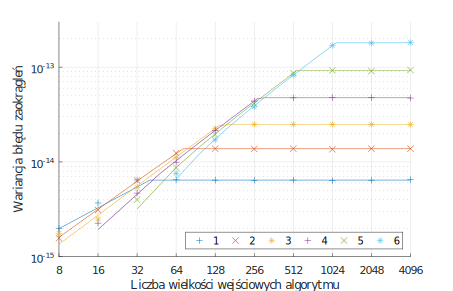
\includegraphics{obrazki/dwt_rerror_coif5}
\makecaption{fig:dwt_rerror_coif5}{Zależność wariancji błędu zaokrągleń od liczby iteracji procesu dekompozycji sygnału oraz liczby wielkości wejściowych dla falki \enquote{coif5} i długości słowa 32-bitów}
\end{center}
\end{figure}

Ze względu na fakt, że dla każdego poziomu dekompozycji wartości współczynników macierzy transformacji są jedynie przesunięte względem poprzedniego wiersza o dwie kolumny, można przyjąć że wariancja błędu zaokrągleń będzie z zadowalającym przybliżeniem stała dla tego samego numeru skali. Cecha ta została potwierdzona podczas przeprowadzania eksperymentu, co zaobserwować można analizując wartości w tabelach \ref{tab:varnum_db2_2_f16} oraz \ref{tab:varnum_db2_2_f32}. Przeprowadzone badania wykazały, że wariancja błędu zaokrągleń jest niemal identyczna dla tego samego numeru skali, poza pierwszą i ostatnią wielkością wyjściową dla tej skali. W przypadku pierwszej i ostatniej wielkości dla tego samego numeru skali zauważyć można największe różnice w kolejności wartości współczynników macierzy transformacji i z tego najpewniej wynika opisywana niewielka różnica w wartości wariancji błędu zaokrągleń.

\begin{table}[htb!]
\begin{center}
\makecaption{tab:varnum_db2_5_f16}{Wariancja błędu zaokrągleń kolejnych grup wielkości wyjściowych algorytmu dyskretnej transformacji falkowej dla falki \enquote{db2} przy pięciu iteracjach procesu dekompozycji, dla liczb o długości 16-bitów, w zależności od liczby wielkości wejściowych}
\begin{tabular}[c]{| c | c | c | c | c | c | c |} \hline
\multirow{2}{*}{$N$} & \multicolumn{6}{ c |}{\textbf{Skala wielkości wyjściowych algorytmu}} \\ \cline{2-7}
& $S_5$ & $T_5$ & $T_4$ & $T_3$ & $T_2$ & $T_1$ \\ \hline
\textbf{64}   & \num{4.91e-7} & \num{5.31e-7} & \num{3.94e-7} & \num{2.09e-7} & \num{1.23e-7} & \num{5.86e-8} \\ \hline
\textbf{128}  & \num{7.51e-7} & \num{7.08e-7} & \num{3.87e-7} & \num{2.07e-7} & \num{1.22e-7} & \num{5.85e-8} \\ \hline
\textbf{256}  & \num{8.59e-7} & \num{6.99e-7} & \num{3.85e-7} & \num{2.05e-7} & \num{1.21e-7} & \num{5.84e-8} \\ \hline
\textbf{512}  & \num{9.19e-7} & \num{6.89e-7} & \num{3.81e-7} & \num{2.04e-7} & \num{1.21e-7} & \num{5.84e-8} \\ \hline
\textbf{1024} & \num{9.47e-7} & \num{6.85e-7} & \num{3.80e-7} & \num{2.04e-7} & \num{1.21e-7} & \num{5.84e-8} \\ \hline
\textbf{2048} & \num{9.58e-7} & \num{6.84e-7} & \num{3.80e-7} & \num{2.04e-7} & \num{1.21e-7} & \num{5.84e-8} \\ \hline
\textbf{4096} & \num{9.66e-7} & \num{6.83e-7} & \num{3.80e-7} & \num{2.04e-7} & \num{1.21e-7} & \num{5.84e-8} \\ \hline
\end{tabular}
\end{center}
\end{table}

\begin{table}[htb!]
\begin{center}
\makecaption{tab:varnum_db2_5_f32}{Wariancja błędu zaokrągleń kolejnych grup wielkości wyjściowych algorytmu dyskretnej transformacji falkowej dla falki \enquote{db2} przy pięciu iteracjach procesu dekompozycji, dla liczb o długości 32-bitów, w zależności od liczby wielkości wejściowych}
\begin{tabular}[c]{| c | c | c | c | c | c | c |} \hline
\multirow{2}{*}{$N$} & \multicolumn{6}{ c |}{\textbf{Skala wielkości wyjściowych algorytmu}} \\ \cline{2-7}
& $S_5$ & $T_5$ & $T_4$ & $T_3$ & $T_2$ & $T_1$ \\ \hline
\textbf{64}   & \num{6.83e-15} & \num{7.93e-15} & \num{5.42e-15} & \num{2.86e-15} & \num{1.62e-15} & \num{7.12e-16} \\ \hline
\textbf{128}  & \num{1.15e-14} & \num{1.02e-14} & \num{5.39e-15} & \num{2.79e-15} & \num{1.58e-15} & \num{6.98e-16} \\ \hline
\textbf{256}  & \num{1.34e-14} & \num{1.03e-14} & \num{5.30e-15} & \num{2.76e-15} & \num{1.56e-15} & \num{6.90e-16} \\ \hline
\textbf{512}  & \num{1.44e-14} & \num{1.03e-14} & \num{5.25e-15} & \num{2.73e-15} & \num{1.55e-15} & \num{6.85e-16} \\ \hline
\textbf{1024} & \num{1.49e-14} & \num{1.03e-14} & \num{5.23e-15} & \num{2.72e-15} & \num{1.55e-15} & \num{6.84e-16} \\ \hline
\textbf{2048} & \num{1.51e-14} & \num{1.03e-14} & \num{5.22e-15} & \num{2.72e-15} & \num{1.55e-15} & \num{6.84e-16} \\ \hline
\textbf{4096} & \num{1.52e-14} & \num{1.03e-14} & \num{5.22e-15} & \num{2.72e-15} & \num{1.55e-15} & \num{6.84e-16} \\ \hline
\end{tabular}
\end{center}
\end{table}

Na podstawie rysunku \ref{fig:dwt_rerror_coif5} zauważyć można liniowy wzrost wariancji błędów zaokrągleń w funkcji liczby wielkości wejściowych, przy czym wzrost ten ustaje gdy przestaje zmieniać się liczba operacji arytmetycznych, tj. dla takiej liczby wielkości wejściowych, która jest równa liczbie niezerowych współczynników skalujących dla analizowanego poziomu dekompozycji sygnału. W przypadku tej samej liczby wielkości wejściowych wariancja błędu rośnie wraz ze wzrostem liczby iteracji procesu dekompozycji sygnału, ponieważ zwiększa się liczba niezerowych współczynników skalujących, a z nią liczba operacji arytmetycznych. Można zatem stwierdzić, że wariancja błędu zaokrągleń związana jest w bezpośrednio z liczbą przeprowadzanych operacji arytmetycznych, która wynika z liczby niezerowych współczynników skalujących odpowiedniej dla wybranej falki oraz liczby wielkości wejściowych algorytmu.

\begin{table}[htb!]
\begin{center}
\makecaption{tab:varnum_spline4_4_5_f16}{Wariancja błędu zaokrągleń kolejnych grup wielkości wyjściowych algorytmu dyskretnej transformacji falkowej dla falki \enquote{spline2:4} przy pięciu iteracjach procesu dekompozycji, dla liczb o długości 16-bitów, w zależności od liczby wielkości wejściowych}
\begin{tabular}[c]{| c | c | c | c | c | c | c |} \hline
\multirow{2}{*}{$N$} & \multicolumn{6}{ c |}{\textbf{Skala wielkości wyjściowych algorytmu}} \\ \cline{2-7}
& $S_5$ & $T_5$ & $T_4$ & $T_3$ & $T_2$ & $T_1$ \\ \hline
\textbf{64}   & \num{1.07e-6} & \num{1.02e-6} & \num{8.94e-7} & \num{5.05e-7} & \num{1.83e-7} & \num{4.76e-8} \\ \hline
\textbf{128}  & \num{1.75e-6} & \num{1.59e-6} & \num{9.22e-7} & \num{4.96e-7} & \num{1.80e-7} & \num{4.64e-8} \\ \hline
\textbf{256}  & \num{2.61e-6} & \num{1.67e-6} & \num{9.11e-7} & \num{4.91e-7} & \num{1.77e-7} & \num{4.58e-8} \\ \hline
\textbf{512}  & \num{2.60e-6} & \num{1.69e-6} & \num{9.05e-7} & \num{4.89e-7} & \num{1.76e-7} & \num{4.55e-8} \\ \hline
\textbf{1024} & \num{2.58e-6} & \num{1.71e-6} & \num{9.02e-7} & \num{4.88e-7} & \num{1.75e-7} & \num{4.53e-8} \\ \hline
\textbf{2048} & \num{2.58e-6} & \num{1.71e-6} & \num{9.00e-7} & \num{4.87e-7} & \num{1.75e-7} & \num{4.53e-8} \\ \hline
\textbf{4096} & \num{2.58e-6} & \num{1.72e-6} & \num{9.00e-7} & \num{4.87e-7} & \num{1.75e-7} & \num{4.53e-8} \\ \hline
\end{tabular}
\end{center}
\end{table}

\begin{table}[htb!]
\begin{center}
\makecaption{tab:varnum_spline4_4_5_f32}{Wariancja błędu zaokrągleń kolejnych grup wielkości wyjściowych algorytmu dyskretnej transformacji falkowej dla falki \enquote{spline2:4} przy pięciu iteracjach procesu dekompozycji, dla liczb o długości 32-bitów, w zależności od liczby wielkości wejściowych}
\begin{tabular}[c]{| c | c | c | c | c | c | c |} \hline
\multirow{2}{*}{$N$} & \multicolumn{6}{ c |}{\textbf{Skala wielkości wyjściowych algorytmu}} \\ \cline{2-7}
& $S_5$ & $T_5$ & $T_4$ & $T_3$ & $T_2$ & $T_1$ \\ \hline
\textbf{64}   & \num{1.51e-14} & \num{1.44e-14} & \num{1.26e-14} & \num{6.54e-15} & \num{2.33e-15} & \num{5.44e-16} \\ \hline
\textbf{128}  & \num{2.52e-14} & \num{2.37e-14} & \num{1.45e-14} & \num{6.50e-15} & \num{2.27e-15} & \num{5.29e-16} \\ \hline
\textbf{256}  & \num{4.72e-14} & \num{2.91e-14} & \num{1.45e-14} & \num{6.40e-15} & \num{2.24e-15} & \num{5.22e-16} \\ \hline
\textbf{512}  & \num{4.72e-14} & \num{2.98e-14} & \num{1.44e-14} & \num{6.36e-15} & \num{2.23e-15} & \num{5.17e-16} \\ \hline
\textbf{1024} & \num{4.71e-14} & \num{3.01e-14} & \num{1.43e-14} & \num{6.35e-15} & \num{2.22e-15} & \num{5.16e-16} \\ \hline
\textbf{2048} & \num{4.72e-14} & \num{3.03e-14} & \num{1.43e-14} & \num{6.35e-15} & \num{2.22e-15} & \num{5.16e-16} \\ \hline
\textbf{4096} & \num{4.72e-14} & \num{3.04e-14} & \num{1.43e-14} & \num{6.35e-15} & \num{2.22e-15} & \num{5.16e-16} \\ \hline
\end{tabular}
\end{center}
\end{table}

Stosowanie liczb rzeczywistych o długości słowa 16-bitów pozwala zmniejszyć czas obliczeń oraz rozmiar wymaganej pamięci w stosunku do analogicznego przypadku wykorzystującego liczby o długości słowa 32-bitów. Wariant ten wprowadza jednak znacznie większe błędy związane z zaokrągleniami ze względu na ograniczoną precyzję. Należy zatem tak dobrać długość słowa, aby błąd zaokrągleń był możliwie mały w stosunku do pozostałych błędów obecnych w przetwarzanym sygnale, przez co w efekcie nie wpływał on znacznie na błąd wypadkowy. Ze względu na fakt, że zakres wielkości wejściowych algorytmu transformacji falkowej również wpływa na wprowadzany błąd zaokrągleń, należy brać ten czynnik pod uwagę podczas analizy projektowanego toru pomiarowego. Należy zatem tak dobrać warunki eksperymentu, aby w jak największym stopniu były one zbieżne z warunkami rzeczywistymi. Analizując przedstawione wyniki zauważyć można, że wraz ze wzrostem zakresu wielkości wejściowych wariancja błędu zaokrągleń wzrasta. Zależność ta wynika bezpośrednio z właściwości stosowanej powszechnie metody zapisu liczb zmiennoprzecinkowych. Analizując przedstawione histogramy zauważyć można, że kształt rozkładu błędów własnych algorytmu jest zbliżony do kształtu rozkładu normalnego, natomiast dla poziomu ufności $\alpha = 95\%$ współczynnik kształtu wynosi około $2.17$. Wobec tego nie można podczas analizy właściwości metrologicznych przyjąć uproszczenia, w którym rozkład błędów zaokrągleń traktowany będzie jak rozkład normalny.

\begin{figure}[htb!]
\begin{center}
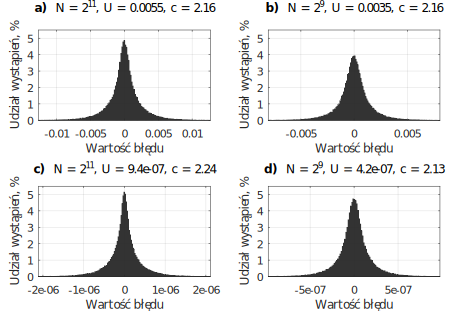
\includegraphics{obrazki/hist_numerr_coif5}
\makecaption{fig:dwt_rhist_coif5}{Histogramy błędu własnego zaokrągleń dla falki \enquote{coif5} przy sześciu iteracjach procesu dekompozycji, dla $N$ wielkości wejściowych, przy długości słowa równej \textbf{a)}, \textbf{b)}~16-bitów, \textbf{c)}, \textbf{d)}~32-bitów}
\end{center}
\end{figure}

\section{Implementacja okna pomiarowego}

Identycznie, jak w przypadku innych algorytmów przetwarzających ciągi wielkości wejściowych, dla algorytmu transformacji falkowej stosować można wybrane okno pomiarowe. Wprowadzenie okna pomiarowego oznaczonego jako $w(n)$ można przedstawić za pomocą modyfikacji równania \eqref{eq:alg_out_single} jako:
\begin{equation}
X \left( i \right) = a_{i, 0} w \left( 0 \right) x \left( 0 \right) + a_{i, 1} w \left( 1 \right) x \left( 1 \right) + \hdots + a_{i, N-1} w \left( N-1 \right) x \left( N-1 \right) \label{eq:wt_singlewindow}.
\end{equation}
Na podstawie przedstawionego równania zauważyć można, że wprowadzenie okna pomiarowego opisać można za pomocą modyfikacji współczynników macierzy transformacji algorytmu zgodnie z zależnością:
\begin{equation}
a_{i,j}^{'} = w \left( j \right) \cdot a_{i,j} \label{eq:wt_windowmod},
\end{equation}
gdzie $a_{i,j}^{'}$ stanowi nową wartość współczynnika macierzy transformacji algorytmu. Użyta funkcja $w(n)$ powinna być opisana dla wartości $n$ w przedziale $<0;N-1>$. Wybrane okna pomiarowe opisane w literaturze \cite{oppenheim_dsp} to okna: trójkątne \eqref{eq:wnd_triang}, Gaussa \eqref{eq:wnd_gauss}, Hamminga \eqref{eq:wnd_hamming} oraz Hanna \eqref{eq:wnd_hann}. W dalszej części pracy stosowane będzie okno prostokątne, w którym $w(n) = 1$ o ile nie zostanie zaznaczony fakt stosowania innego okna pomiarowego. Wpływ parametrów okna pomiarowego na przenoszenie błędów losowych przez algorytmy dyskretnej transformacji falkowej przedstawiono w pracy \cite{auth_window}. Wymienione funkcje okien przedstawiają równania:
\begin{gather}
w_{\text{tr}} \left( n \right) = 1 - \left| \frac{n - \frac{N-1}{2}}{\frac{N}{2}} \right| \label{eq:wnd_triang}, \\
w_{\text{ga}} \left( n \right) = \exp \left(-\frac{1}{2} \cdot \left( \frac{n - \frac{N-1}{2}}{\sigma \frac{ \left( N-1 \right)}{2}} \right)^{2} \right) \label{eq:wnd_gauss}, \\
w_{\text{hm}} \left( n \right) = 0.5384 - 0.4616 \cos \left( \frac{2 \pi n}{N} \right) \label{eq:wnd_hamming}, \\
w_{\text{hn}} \left( n \right) = 0.5 \left(1 - \cos \left( \frac{2 \pi n}{N} \right) \right) \label{eq:wnd_hann},
\end{gather}

Implementacja okna pomiarowego, z punktu widzenia przedstawionych w pracy założeń, mogłaby również zostać opisana jako zastosowanie dodatkowego algorytmu. Algorytm ten przetwarzałby $N$ wielkości wejściowych na $M$ wielkości wyjściowych, gdzie $N = M$. Macierz transformacji omawianego algorytmu byłaby macierzą diagonalną, przy czym wartości kolejnych współczynników odpowiadałyby wyznaczonym wagom dla $i$-tej wielkości okna. Z praktycznego punktu widzenia zaproponowana metoda modyfikacji wartości współczynników transformacji algorytmu transformacji falkowej wydaje się jednak bardziej optymalna. Na tej samej zasadzie istnieje możliwość implementacji innych modyfikacji, np. wprowadzenia dodatkowego filtru.

\chapter{Symulacyjna weryfikacja tezy}

Weryfikacja przedstawionego w pracy modelu błędów i wynikających z niego założeń w pierwszej kolejności przeprowadzona została metodą symulacyjną. W bieżącym rozdziale przedstawiono przykładowy tor pomiarowy, a następnie wymieniono i opisano obecne w nim źródła błędów. Na podstawie przedstawionego wcześniej modelu błędów opisano związki zachodzące pomiędzy zidentyfikowanymi sygnałami błędów oraz oszacowano wartości niepewności rozszerzonych wielkości wyjściowych analizowanego toru pomiarowego. Wyniki uzyskane za pomocą zaproponowanego modelu porównano z wynikami uzyskanymi metodą Monte Carlo. Aby zapewnić możliwość bieżącej weryfikacji poprawności stosowanych założeń, podczas analizy wyznaczano wartości dla wszystkich wyprowadzanych wielkości, co umożliwiało porównywanie uzyskanych wyników z wynikami symulacji uzyskiwanymi metodą Monte Carlo. Wybrane wartości liczbowe dla analizowanych wielkości przedstawiano jedynie w celu możliwości weryfikacji każdego etapu analizy, natomiast ostateczne wyniki wyznaczane były na podstawie wyprowadzonych wcześniej zależności.

Przykładowy tor pomiarowy składa się z przetwornika pomiarowego, który przekształca ciągłą w czasie fizyczną wielkość mierzoną $s(t)$ na reprezentujący ją sygnał napięciowy $y_{a}(t)$, który następnie przetwarzany jest przez wzmacniacz pomiarowy, w celu dopasowania jego poziomu do zakresu napięcia wejściowego zintegrowanego z układem próbkująco-pamiętającym przetwornika analogowo-cyfrowego. Wzmocniony sygnał $y_{b}(t)$ stanowi wejście przetwornika analogowo-cyfrowego, którego wielkości wyjściowe wyrażone w jednostce wielkości $y_{b}(t)$ oznaczono symbolem $x_{c}(i)$. Ostatecznie sygnał wyjściowy przetwornika analogowo-cyfrowego trafia na wejście algorytmu dyskretnej transformacji falkowej, a na jego podstawie wyznaczany jest wektor wielkości wyjściowych, oznaczonych jako $\mathbfit{X}(k)$. Schemat blokowy opisanego toru pomiarowego przedstawiono na rysunku~\ref{fig:chain_symul}. Podczas eksperymentu przyjęto, że przetwarzany sygnał pomiarowy obarczony jest błędem związanym z szumem białym o stałej widmowej gęstości mocy. Przetwornik pomiarowy, zastosowany w celu przetworzenia analizowanego sygnału wejściowego na postać napięciową, cechuje się pewną częstotliwość graniczną, a jego charakterystyka nie jest idealnie liniowa. Zastosowany wzmacniacz pomiarowy również charakteryzuje się pewną częstotliwością graniczną, natomiast założono, że nieliniowość charakterystyki jest w jego przypadku pomijalnie mała. Przyjęto, że temperatura otoczenia miała wpływ na dryft zera przetwornika pomiarowego oraz wzmacniacza, przy czym temperatura ta nie była mierzona, zatem jej wpływ na wyniki pomiarów nie był korygowany. Przyjęto, że zastosowany przetwornik analogowo-cyfrowy wprowadzał do sygnału wyjściowego jedynie błąd związany z kwantowaniem przetwarzanej wielkości, natomiast algorytm transformacji falkowej wprowadzał do wielkości wyjściowych błąd własny związany z wykonywaniem operacji arytmetycznych.

\begin{figure}[htb!]
\begin{center}
\includegraphics{obrazki/schemat_symul}
\makecaption{fig:chain_symul}{Schemat blokowy toru pomiarowego będącego obiektem eksperymentu symulacyjnego, gdzie symbol \enquote{A/A} oznacza przetwarzanie analogowo-analogowe, \enquote{A/C} przetwarzanie analogowo-cyfrowe, natomiast \enquote{DWT} algorytm dyskretnej transformacji falkowej}
\end{center}
\end{figure}

W dalszej części rozdziału omówiono kolejne elementy toru pomiarowego, wskazano ich wpływ na przetwarzany sygnał oraz relacje pomiędzy sygnałami błędów na wejściu i wyjściu tych fragmentów. Przedstawiono również szczegółowe założenia odnośnie właściwości opisanych we wprowadzeniu fragmentów toru pomiarowego. Dla przeprowadzonego eksperymentu przyjęto, że przetwarzany sygnał $s(t)$ określony został w dziedzinie czasu jako:
\begin{gather}
\dot{s} \emb{t} = \frac{6}{10} \sin \left( 2 \pi f_{1} t \right) - \frac{3}{10} \sin \left( 10 \pi f_{1} t + \frac{\pi}{8} \right) + \frac{1}{10} \sin \left( 30 \pi f_{1} t + \frac{\pi}{6} \right) \label{eq:sym_in_ideal}, \\
\tilde{s} \emb{t} = \dot{s} \emb{t} + e_{s,r} \emb{t} = e_{s,r} \emb{t} + \sum _{i=1} ^{3} E_{s,o} \emb{\omega_{s,i}} \sin \emb{\omega_{s,i} t + \varphi_{s,i}} \label{eq:sym_in_real},
\end{gather}
przy czym $f_{1} = \qty{1}{kHz}$ jest częstotliwością podstawowej harmonicznej tego sygnału, natomiast $\sigma_{s,r}^{2}(\omega) = \frac{2}{3} \cdot 10^{-5}$ wariancją sygnału szumu $e_{s,r}(t)$. Parametry kolejnych harmonicznych przetwarzanego sygnału zostały zestawione w tabeli~\ref{tab:sym_in_params_ideal}. Do wyznaczenia wektora wielkości wyjściowych algorytmu dyskretnej transformacji falkowej koniecznych było $N = 8$ próbek wielkości wejściowych $x_{c}(i)$ tego algorytmu, na podstawie których wyznaczano $M = 8$ próbek wektora wielkości wyjściowych $\mathbfit{X}(k)$ obiektu dla każdej $k$-tej realizacji pomiaru. Eksperyment zakładał stały dla każdej $i$-tej próbki przetwarzanego sygnału okres próbkowania $T_{p} = \frac{1}{f_{s}}$, gdzie $f_{s} = \qty{48}{kHz}$, natomiast okno pomiarowe usytuowane było losowo względem przebiegu przetwarzanego sygnału $s(t)$. Założono, że temperatura otoczenia $\vartheta(t)$ przyjmowała w funkcji czasu dowolną wartość z zakresu $\hat{\vartheta}(t) \in \interval{17}{23}~\unit{\degreeCelsius}$, wartością oczekiwaną temperatury była wartość~\qty{20}{\degreeCelsius} oraz w obrębie wskazanego przedziału rozkład wartości tej wielkości był rozkładem trójkątnym.

\begin{table}[htb!]
\begin{center}
\makecaption{tab:sym_in_params_ideal}{Parametry kolejnych harmonicznych przetwarzanego sygnału $s(t)$ dla sytuacji idealnej, przyjęte w przeprowadzanym eksperymencie symulacyjnym}
\begin{tabular}[c]{| c | c | c | c |} \hline
\textbf{$i$} & \textbf{Pulsacja $\omega_{s,i}$, rad/s} & \textbf{Amplituda $E_{s,o}(\omega_{s,i})$} & \textbf{Faza $\varphi_{s,o}(\omega_{s,i})$, rad} \\ \hline
1 & $1000  \cdot 2\pi$ &  \num{0.6} & $0$           \\ \hline
2 & $5000  \cdot 2\pi$ &  \num{0.3} & $\pi/8 + \pi$ \\ \hline
3 & $15000 \cdot 2\pi$ &  \num{0.1} & $\pi/6$       \\ \hline
\end{tabular}
\end{center}
\end{table}

\section{Analiza przetwornika pomiarowego}

Zastosowany przetwornik pomiarowy przekształca sygnał $s(t)$, związany z mierzoną wielkością fizyczną, na wyjściowy sygnał napięciowy $y_{a}(t)$. Przyjęto, że wartości realizacji wielkości mierzonej zawierają się w zakresie $\hat{s}(t) \in \interval{0}{1}$, natomiast czułość przetwornika pomiarowego jest równa $s_{a} = \qty{1}{V \per 1}$, związana z nim częstotliwość graniczna wynosi $f_{a,g} = \qty{320}{kHz}$. Wobec powyższych, wartości realizacji wielkości wyjściowej $y_{a}(t)$ mieszczą się w przedziale $\hat{y}_{a}(t) \in \interval{0}{1}~\unit{V}$. Charakterystyka omawianego obiektu jest zależna od temperatury otoczenia $\vartheta(t)$, przy czym jej wartość nie jest znana.

Stosując zaproponowany model błędów i przedstawione założenia, na podstawie równań~\eqref{eq:out_cont_ideal_all} oraz~\eqref{eq:out_cont_real_all}, opisać można przebieg wielkości wyjściowej $y_{a}(t)$ jako:
\begin{gather}
\dot{y}_{a} \emb{t} = \dot{f}_{a} \emb{\dot{s} \emb{t}} = \dot{s} \emb{t} \label{eq:sym_parta_out_ideal}, \\
\tilde{y}_{a} \emb{t} = \dot{y}_{a} \emb{t} + e_{a,\Sigma} \emb{t} \label{eq:sym_parta_out_real},
\end{gather}
przy czym sygnały błędów zawarte w sygnale błędu wypadkowego $e_{a,\Sigma}(t)$ zdefiniowano i omówiono w dalszej cześć podrozdziału. Funkcja przetwarzania obiektu $f_{a}(x)$ powinna być zatem w przypadku idealnym, zgodnie z założeniami opisanymi zależnością~\eqref{eq:sym_parta_out_ideal} oraz wymienionymi we wstępie podrozdziału, określona równaniem w postaci:
\begin{equation}
\dot{f}_{a} \emb{x} = s_{a} x = x \label{eq:sym_parta_statfun}.
\end{equation}
Przyjmuje się, że rzeczywista funkcja przetwarzania obiektu $\tilde{f}_{a}(x)$ nie jest znana, natomiast realizacje sygnału błędu $e_{a,zw}(t)$ wynikającego z nieliniowości charakterystyki przyjmują wartości z przedziału $\hat{e}_{a,fw}(t) \in \interval{-\sqrt{10}}{\sqrt{10}}~\unit{mV}$, a uzyskanie każdej z nich jest jednakowo prawdopodobne. Zakłada się, że charakter rozważanego sygnału błędu jest zbliżony do charakteru sygnału błędu kwantowania, zatem błąd ten zaliczyć można do grupy sygnałów błędów losowych. Wariancję oraz niepewność rozszerzoną, związane z omawianym sygnałem błędu $e_{a,rw}(t) = e_{a,fw}(t)$, wyrazić można w postaci~\cite{jcgm_guide}:
\begin{gather}
\sigma_{a,rw}^{2} = \frac{\left( \left( \sqrt{10} \cdot 10^{-3} \right) + \left( \sqrt{10} \cdot 10^{-3} \right) \right)^{2}}{12} = 3 \frac{1}{3}~\unit{\micro V} \label{eq:sym_parta_rand_self_var}, \\
U_{a,rw} = c_{u} \sigma_{a,rw} = \frac{\num{1.65} \sqrt{30}}{3}~\unit{mV} \label{eq:sym_parta_rand_self_unc},
\end{gather}
przy czym $c_{u}$ jest współczynnikiem rozszerzenia dla rozkładu jednostajnego i przy poziomie ufności $\gamma = \qty{95}{\percent}$ wynosi~\num{1.65}. Ze względu na nieznaną postać rzeczywistej funkcji przetwarzania, w dalszych rozważaniach przyjmuje się, że $\tilde{f}_{a}(x)  \cong  \dot{f}_{a}(x)$.

Zmiany temperatury otoczenia, ujęte w założeniach eksperymentu, rozważać można jako bardzo niewielkie w obrębie pojedynczej serii pomiarowej (dla $k$-tego okna pomiarowego). Można zatem przyjąć, że błąd wynikający z wpływu tej temperatury na wartość wielkości wyjściowej analizowanego obiektu jest niezmienny w obrębie pojedynczego okna pomiarowego, a zatem, zgodnie z przyjętym modelem, kwalifikować go można jako błąd statyczny. Sygnał błędu statycznego własnego $e_{a,sw}(t)$ związany z omawianym zjawiskiem, zgodnie z równaniem~\eqref{eq:out_cont_err_env_self} jest zatem zdefiniowany jako:
\begin{equation}
e_{a,sw} \emb{t} = f_{a,z} \left( \vartheta \emb{t} \right) = \frac{3}{2} \left( \vartheta \emb{t} - \qty{20}{\degreeCelsius} \right)~\unit{\frac{mV}{K}} \label{eq:sym_parta_stat_err},
\end{equation}
gdzie $\vartheta(t)$ jest rzeczywistą temperaturą otoczenia wyrażoną w stopniach Celsjusza. Można zatem określić wariancję oraz niepewność rozszerzoną omawianego sygnału~\cite{jcgm_guide}:
\begin{gather}
\sigma_{a,sw}^{2} = \frac{\left( -\frac{9}{2} \cdot 10^{-3} \right)^{2} + \left( \frac{9}{2} \cdot 10^{-3} \right)^{2} - \left( -\frac{9}{2} \cdot 10^{-3} \right) \left( \frac{9}{2} \cdot 10^{-3} \right)}{18} = 3 \frac{3}{8}~\unit{\micro V} \label{eq:sym_parta_stat_var}, \\
U_{a,sw} = c_{t} \sigma_{a,rw} = \frac{\num{5.7} \sqrt{6}}{4}~\unit{mV} \label{eq:sym_parta_stat_unc},
\end{gather}
gdzie $c_{t}$ jest współczynnikiem rozszerzenia dla rozkładu trójkątnego i przy poziomie ufności $\gamma = \qty{95}{\percent}$ wynosi~\num{1.90}.

Kolejną grupę właściwości obiektu stanowią właściwości dynamiczne, związane z jego częstotliwością graniczną. Przypadek idealny zakłada, że analizowany obiekt nie powinien mieć żadnego wpływu na widmo przetwarzanego sygnału, a zatem transmitancja tego obiektu powinna wynosić $\dot{G}_{a}(j\omega) = 1$. Na podstawie założonych parametrów rzeczywistych obiektu przyjmuje się, że transmitancja $\tilde{G}_{a}(j\omega)$ wynosi:
\begin{equation}
\tilde{G}_{a} \emb{j\omega} = \frac{1}{1 + j \frac{\omega}{2 \pi f_{a,g}}} = \frac{1}{\frac{\omega^{2}}{4 \pi^{2} f_{a,g}^{2}} + 1} - j \frac{\omega}{2 \pi f_{a,g} \left( \frac{\omega^{2}}{4 \pi^{2} f_{a,g}^{2}} + 1 \right) } \label{eq:sym_parta_trans},
\end{equation}
zatem równania~\eqref{eq:mid_cont_amp} oraz~\eqref{eq:mid_cont_phi}, określające właściwości dynamiczne, przyjmują postać:
\begin{gather}
\tilde{K}_{a} \emb{\omega} = \sqrt{\left( \Re \left( \tilde{G}_{a} \emb{j\omega} \right) \right)^{2} + \left( \Im \left( \tilde{G}_{a} \emb{j\omega} \right) \right)^{2}} = \left( \frac{\omega^{2}}{4 \pi^{2} f_{a,g}^{2}} + 1 \right)^{-\frac{1}{2}} \label{eq:sym_parta_amp_real}, \\
\tilde{\varphi}_{a} \emb{\omega} = \arctan \left( \frac{\Im \left( \tilde{G}_{a} \emb{j\omega} \right)}{\Re \left( \tilde{G}_{a} \emb{j\omega} \right)} \right) = \arctan \left( -\frac{\omega}{2 \pi f_{a,g}} \right) \label{eq:sym_parta_phi_real}, \\
\dot{K}_{a} \emb{\omega} = \sqrt{\left( \Re \left( \dot{G}_{a} \emb{j\omega} \right) \right)^{2} + \left( \Im \left( \dot{G}_{a} \emb{j\omega} \right) \right)^{2}} = \qty{1}{V \per 1} \label{eq:sym_parta_amp_ideal}, \\
\dot{\varphi}_{a} \emb{\omega} = \arctan \left( \frac{\Im \left( \dot{G}_{a} \emb{j\omega} \right)}{\Re \left( \dot{G}_{a} \emb{j\omega} \right)} \right) = \qty{0}{rad} \label{eq:sym_parta_phi_ideal}.
\end{gather}

Na podstawie powyższych zależności określających parametry transmitancji obiektu w sytuacji idealnej, a także założeń~\eqref{eq:mid_cont_omega_ideal}, \eqref{eq:mid_cont_sum_ideal}, \eqref{eq:out_cont_ideal_all} oraz~\eqref{eq:sym_parta_out_ideal}, opisać można idealne parametry kolejnych harmonicznych sygnału $y_{a}(t)$ w funkcji pulsacji jako:
\begin{gather}
E_{a,o} \emb{\omega} = s_{a} \dot{K}_{a} \emb{\omega} E_{s,o} \emb{\omega} = E_{s,o} \emb{\omega} \label{eq:sym_parta_amp_out_ideal}, \\
\varphi_{a,o} \emb{\omega} = \varphi_{s,o} \emb{\omega} + \dot{\varphi}_{a} \emb{\omega} = \varphi_{s,o} \emb{\omega} \label{eq:sym_parta_phi_out_ideal},
\end{gather}
gdzie $E_{a,o}(\omega)$ jest idealną amplitudą oraz $\varphi_{a,o}(\omega)$ idealną fazą harmonicznej sygnału wyjściowego $y_{a}(t)$ o wybranej pulsacji $\omega$. Wskazane zależności oraz definicja przetwarzanego sygnału wejściowego, dana równaniem~\eqref{eq:sym_in_ideal}, umożliwiają definicję opisanej równaniem~\eqref{eq:sym_parta_out_ideal} wielkości wyjściowej obiektu dla przypadku idealnego w postaci sumy analizowanych harmonicznych tego sygnału:
\begin{equation}
\dot{y}_{a} \emb{t} = \sum _{i=1} ^{3} E_{a,o} \emb{\omega_{a,i}} \sin \emb{\omega_{a,i} t + \varphi_{a,i}} \label{eq:sym_parta_out_ideal_sum},
\end{equation}
przy czym $\omega_{a,i} = \omega_{s,i}$ jest pulsacją $i$-tej harmonicznej sygnału wyjściowego, której kolejne parametry zestawione zostały wcześniej w tabeli~\ref{tab:sym_in_params_ideal}. Parametry sygnału opisanego równaniem~\eqref{eq:sym_parta_out_ideal_sum} zestawiono w tabeli~\ref{tab:sym_outa_params_ideal}.

\begin{table}[htb!]
\begin{center}
\makecaption{tab:sym_outa_params_ideal}{Parametry kolejnych harmonicznych sygnału $y_{a}(t)$ przyjęte w przeprowadzanym eksperymencie symulacyjnym dla sytuacji idealnej}
\begin{tabular}[c]{| c | c | c | c |} \hline
\textbf{$i$} & \textbf{Pulsacja $\omega_{a,i}$, rad/s} & \textbf{Amplituda $E_{a,o}(\omega_{a,i})$, V} & \textbf{Faza $\varphi_{a,o}(\omega_{a,i})$, rad} \\ \hline
1 & $1000  \cdot 2\pi$ &  \num{0.6} & $0$             \\ \hline
2 & $5000  \cdot 2\pi$ &  \num{0.3} & $\pi/8 + \pi$   \\ \hline
3 & $15000 \cdot 2\pi$ &  \num{0.1} & $\pi/6$         \\ \hline
\end{tabular}
\end{center}
\end{table}

Na podstawie równań~\eqref{eq:mid_cont_err_dyn_self} oraz~\eqref{eq:out_cont_err_dyn_self}, błąd własny dynamiczny w funkcji pulsacji wybranej harmonicznej sygnału opisać można następującą zależnością:
\begin{equation}
\begin{split}
e_{a,dw} \emb{t,\omega} =~
& \tilde{f}_{a} \emb{\tilde{K}_{a} \emb{\omega} E_{s,o} \emb{\omega} \sin \left( \omega t + \varphi_{s,o} \emb{\omega} + \tilde{\varphi}_{a} \emb{\omega} \right)} - \\
& \tilde{f}_{a} \emb{\dot{K}_{a} \emb{\omega} E_{s,o} \emb{\omega} \sin \left( \omega t + \varphi_{s,o} \emb{\omega} + \dot{\varphi}_{a} \emb{\omega} \right)}
\end{split}
\label{eq:sym_parta_dyn_self_err}.
\end{equation}
Jako że sygnał wejściowy $s(t)$ analizowanego obiektu nie jest obarczony błędem dynamicznym, nie ma potrzeby wykonywania analizy dla sygnału błędu dynamicznego propagowanego. Aby umożliwić analizę propagacji sygnałów błędów dynamicznych przez kolejne fragmenty toru pomiarowego, minimalizując jednocześnie liczbę analizowanych składowych błędu dynamicznego, wyznaczono na podstawie równań~\eqref{eq:dyn_vect_amp} oraz~\eqref{eq:dyn_vect_phi} wypadkowe parametry amplitudy oraz fazy dla kolejnych harmonicznych tego sygnału. Należy zauważyć, że relacje pomiędzy amplitudą i wariancją analizowanej harmonicznej opisuje równanie~\eqref{eq:dyn_var}. Analizując równanie~\eqref{eq:sym_parta_dyn_self_err} można zauważyć, że dla każdej harmonicznej błąd ten ma dwie składowe o przeciwnych znakach. Korzystając z właściwości funkcji \enquote{sinus} można odwrócić znak wybranej składowej oraz dodać kąt $\pi~\unit{rad}$ do argumentu tej funkcji, zachowując przy tym oryginalną wartość tej składowej.

Stosując podane założenia, przebieg składowej sygnału błędu dynamicznego własnego o częstotliwości~\qty{1}{kHz} przedstawić można następującym równaniem:
\begin{equation}
\begin{split}
e_{a,dw} \emb{t,\omega} \left|_{\omega = 1000 \cdot 2 \pi} \right. =~
& \tilde{f}_{y} \emb{\tilde{K}_{a} \emb{\omega} E_{s,o} \emb{\omega} \sin \left( \omega t + \varphi_{s,o} \emb{\omega} + \tilde{\varphi}_{a} \emb{\omega} \right)} - \\
& \tilde{f}_{y} \emb{\dot{K}_{a} \emb{\omega} E_{s,o} \emb{\omega} \sin \left( \omega t + \varphi_{s,o} \emb{\omega} + \dot{\varphi}_{a} \emb{\omega} \right)} = \\
& \num{1.0} \cdot \num{0.6} \sin \left( 1000 \cdot 2 \pi t + 0 - \num{3.13e-3} \right) + \\
& \num{1.0} \cdot \num{0.6} \sin \left( 1000 \cdot 2 \pi t + 0 + 0 + \pi \right)
\end{split}
\label{eq:sym_parta_dyn_self_example_harm},
\end{equation}
przy czym opisane w podany sposób parametry kolejnych harmonicznych sygnału błędu dynamicznego zestawiono w tabeli~\ref{tab:sym_parta_params_dyn_list}. Przedstawiając składowe równania~\eqref{eq:sym_parta_dyn_self_example_harm} za pomocą wektorów, zgodnie z równaniem~\eqref{eq:dyn_vect}, a następnie zgodnie z równaniem~\eqref{eq:dyn_vect_sum} sumując opisane składniki, wyznaczyć można wypadkowe parametry harmonicznych sygnału błędu $e_{a,dw}(t)$ zgodnie z zależnościami~\eqref{eq:dyn_vect_amp} oraz~\eqref{eq:dyn_vect_phi}. Dla przedstawionej w równaniu~\eqref{eq:sym_parta_dyn_self_example_harm} harmonicznej sygnału błędu dynamicznego, parametry te wynoszą:
\begin{gather}
\mathbfit{e}_{a,e,1} =
\begin{bmatrix}
\num{0.6} \cos \emb{\num{-3.13e-3}} + \num{0.6} \cos \emb{\pi} & \num{0.6} \sin \emb{\num{-3.13e-3}} + \num{0.6} \sin \emb{\pi}
\end{bmatrix}
\label{eq:sym_parta_dyn_self_example_sum}, \\
E_{a,e} \emb{\omega}\left|_{\omega = 1000 \cdot 2 \pi}\right. = E_{\Sigma,a,e,1} = \sqrt{\emb{\num{-5.86e-6}}^{2} + \emb{\num{-1.88e-3}}^{2}} = \qty{1.88}{mV} \label{eq:sym_parta_dyn_self_example_amp}, \\
\varphi_{a,e} \emb{\omega}\left|_{\omega = 1000 \cdot 2 \pi}\right. = \varphi_{\Sigma,a,e,1} = \arctan \emb{\frac{\num{-1.88e-3}}{\num{-5.86e-6}}} = \qty{-1.57}{rad} \label{eq:sym_parta_dyn_self_example_phi}.
\end{gather}
Dla pozostałych harmonicznych należy opisane powyżej wielkości wyznaczyć w sposób analogiczny, przy czym wartości tych wielkości zestawiono w tabeli~\ref{tab:sym_parta_params_dyn_summary}. Na podstawie równania~\eqref{eq:dyn_var} możliwe jest wyznaczenie wartości wariancji kolejnych składowych błędu dynamicznego oraz na podstawie równania~\eqref{eq:unc_sum} wartości ich niepewności rozszerzonej:
\begin{gather}
\sigma_{a,dw,1}^{2} = \frac{E_{a,e,1}^{2}}{2} = \qty{1.77}{\micro V} \label{eq:sym_parta_dyn_self_var}, \\
U_{a,dw,1} = c_{d} \sigma_{a,dw,1} = \qty{1.87}{mV} \label{eq:sym_parta_dyn_self_unc},
\end{gather}
przy czym dla rozkładu dwumodalnego współczynnik rozszerzenia $c_{d}$ dla deklarowanego poziomu ufności $\gamma = \qty{95}{\percent}$ jest równy~\num{1.41}~\cite{jakubiec_system, jcgm_guide}.

\begin{table}[htb!]
\begin{center}
\makecaption{tab:sym_parta_params_dyn_list}{Parametry składowe kolejnych harmonicznych błędu dynamicznego własnego analizowanego w eksperymencie symulacyjnym przetwornika pomiarowego}
\begin{tabular}[c]{| c | c | c | c | c |} \hline
\textbf{$i$} & \textbf{$j$} & \textbf{Pulsacja $\omega_{a,i}$, rad/s} & \textbf{Amplituda $E_{a,e,j}(\omega_{a,i})$, V} & \textbf{Faza $\varphi_{a,e,j}(\omega_{a,i})$, rad} \\ \hline
\multirow{2}{*}{$1$} & 1 & \multirow{2}{*}{$1000  \cdot 2\pi$} &  $\num{1.0} \cdot \num{0.6}$ & $0 - \num{3.13e-3}$            \\ \cline{2-2} \cline{4-5}
                     & 2 &                                     &  $\num{1.0} \cdot \num{0.6}$ & $0 + 0 + \pi$                  \\ \hline
\multirow{2}{*}{$2$} & 1 & \multirow{2}{*}{$5000  \cdot 2\pi$} &  $\num{1.0} \cdot \num{0.3}$ & $\pi/8 - \num{1.56e-2} + \pi$  \\ \cline{2-2} \cline{4-5}
                     & 2 &                                     &  $\num{1.0} \cdot \num{0.3}$ & $\pi/8 + 0$                    \\ \hline
\multirow{2}{*}{$3$} & 1 & \multirow{2}{*}{$15000 \cdot 2\pi$} &  $\num{1.0} \cdot \num{0.1}$ & $\pi/6 - \num{4.69e-2}$        \\ \cline{2-2} \cline{4-5}
                     & 2 &                                     &  $\num{1.0} \cdot \num{0.1}$ & $\pi/6 + 0 + \pi$              \\ \hline
\end{tabular}
\end{center}
\end{table}

\begin{table}[htb!]
\begin{center}
\makecaption{tab:sym_parta_params_dyn_summary}{Parametry wypadkowe kolejnych harmonicznych błędu dynamicznego własnego analizowanego w eksperymencie symulacyjnym przetwornika pomiarowego}
\begin{tabular}[c]{| c | c | S[table-format = 1.2] | S[table-format = +1.2] |} \hline
\textbf{$i$} & \textbf{Pulsacja $\omega_{a,i}$, rad/s} & \textbf{Amplituda $E_{a,e}(\omega_{a,i})$, mV} & \textbf{Faza $\varphi_{a,e}(\omega_{a,i})$, rad} \\ \hline
1 & $1000  \cdot 2\pi$  &  1.88  & -1.57  \\ \hline
2 & $5000  \cdot 2\pi$  &  4.69  &  1.96  \\ \hline
3 & $15000 \cdot 2\pi$  &  4.68  & -1.07  \\ \hline
\end{tabular}
\end{center}
\end{table}

Wyprowadzone dotychczas zależności oraz dane zestawione w tabeli~\ref{tab:sym_parta_params_dyn_summary} pozwalają zgodnie z równaniem~\eqref{eq:mid_cont_err_dyn_self} zdefiniować wypadkowy sygnał błędu dynamicznego własnego w postaci sumy kolejnych harmonicznych tego sygnału:
\begin{equation}
e_{a,dw} \emb{t} = \sum _{i=1} ^{3} E_{a,e} \emb{\omega_{a,i}} \sin \emb{\omega_{a,i} t + \varphi_{a,e} \emb{\omega_{a,i}}} \label{eq:sym_parta_dyn_self_sum}.
\end{equation}
Należy zauważyć, że ze względu na fakt, że sygnał ten będzie przetwarzany przez kolejne fragmenty toru pomiarowego, dalsza analiza wykorzystująca wypadkowe parametry kolejnych harmonicznych tego sygnału wydaje się być najbardziej przystępna.

Ostatnim sygnałem błędu wymagającym analizy jest sygnał $e_{a,rp}(t)$, związany z szumem na wejściu obiektu. Wariancję tego sygnału w funkcji pulsacji określić można stosując kolejno zależności~\eqref{eq:mid_cont_var_omega} oraz~\eqref{eq:out_cont_var_sense}, a zatem:
\begin{equation}
\sigma_{a,rp}^{2} \emb{\omega} = s_{a}^{2} \tilde{K}_{a}^{2} \emb{\omega} \sigma_{s,r}^{2} \emb{\omega} \label{eq:sym_parta_rand_prop_var_omega}.
\end{equation}
Jako że w zakresie częstotliwości $\hat{f} \in \interval{0}{\frac{1}{2} f_{p}}$ wartość wzmocnienia $\tilde{K}_{a}(\omega)$ jest zbliżona do jedności, transmitancja obiektu nie wpływa na widmo przetwarzanego sygnału szumu. Zasadne jest zatem założenie, że wariancja sygnału błędu losowego propagowanego w funkcji pulsacji jest identyczna, jak na wejściu obiektu dla analizowanego zakresu częstotliwości, stąd $\sigma_{a,rp}^{2}(\omega) \cong \sigma_{s,r}^{2}(\omega) = \frac{20}{3}~\unit{\micro V}$. Niepewność rozszerzoną związaną z opisywanym sygnałem wyznaczyć można zatem zgodnie z zależnością~\eqref{eq:unc_sum}:
\begin{equation}
U_{a,rp} = c_{u} \sigma_{a,rp} = \frac{\num{3.92} \sqrt{15}}{3}~\unit{mV} \label{eq:sym_parta_rand_prop_unc},
\end{equation}
gdzie $c_{u}$ to współczynnik rozszerzenia rozkładu normalnego, równy~\num{1.96} dla $\gamma = \qty{95}{\percent}$.

Zdefiniowane dotychczas sygnały błędów stanowią kolejne składniki wypadkowego sygnału błędu $e_{a,\Sigma}(t)$ wielkości wyjściowej analizowanego obiektu, wprowadzonego wcześniej w równaniu~\eqref{eq:sym_parta_out_real}. Ostatecznie, sygnał ten opisać można w postaci:
\begin{equation}
e_{a,\Sigma} \emb{t} = e_{a,sw} \emb{t} + e_{a,rw} \emb{t} + e_{a,rp} \emb{t} + e_{a,dw} \emb{t} \label{eq:sym_parta_error_sum}.
\end{equation}
Na podstawie parametrów wymienionych sygnałów określono budżet niepewności dla analizowanego fragmentu toru pomiarowego, który zestawiono w tabeli~\ref{tab:sym_parta_params_unc_list}. Należy zauważyć, że kolejne sygnały błędów w opisywanym przypadku nie są skorelowane.

\begin{table}[htb!]
\begin{center}
\makecaption{tab:sym_parta_params_unc_list}{Budżet niepewności wielkości wyjściowej analizowanego w eksperymencie symulacyjnym przetwornika pomiarowego}
\begin{tabular}[c]{| c | c | S[table-format = 1.2] | S[table-format = 2.2] | c | c |} \hline
\textbf{Lp.} & \textbf{Symbol} & \textbf{$U$, mV} & \textbf{$\sigma^{2}$, \micro V} & \textbf{Rozkład} & \textbf{Źródło błędu} \\ \hline
1 & ${a,sw}$       & 3.49  &  3.38   & trójkątny                    & dryft temperatury                           \\ \hline
2 & ${a,rw}$       & 3.01  &  3.33   & jednostajny                  & nieliniowość obiektu                        \\ \hline
3 & ${a,rp}$       & 5.06  &  6.67   & normalny                     & szum wielkości wejściowej                   \\ \hline
4 & ${a,dw,1}$     & 1.87  &  1.77   & \multirow{3}{*}{dwumodalny}  & \multirow{3}{*}{transmitancja przetwornika} \\ \cline{1-4}
5 & ${a,dw,2}$     & 4.68  &  11.00  &                              &                                             \\ \cline{1-4}
6 & ${a,dw,3}$     & 4.67  &  10.95  &                              &                                             \\ \hline
\end{tabular}
\end{center}
\end{table}

Ostatnim możliwym krokiem pozostaje zatem określenie wartości wypadkowej niepewności rozszerzonej dla analizowanego fragmentu toru pomiarowego. Na obecnym etapie rozważań wyznaczanie tego parametru nie jest konieczne i nie będzie wykorzystywane w dalszym procesie analizy -- przeprowadzenie tej operacji jest jednak uzasadnione potrzebą weryfikacji skuteczności proponowanej metody wyznaczania wartości wypadkowej niepewności rozszerzonej, opisanej równaniem~\eqref{eq:unc_matrix}.

Uwzględniając podział rodzajów sygnałów błędów zorientowany ze względu na charakter ich realizacji, równanie~\eqref{eq:sym_parta_error_cat} zapisać można również w postaci:
\begin{gather}
e_{a,\Sigma} \emb{t} = e_{a,s} \emb{t} + e_{a,d} \emb{t} + e_{a,r} \emb{t} \label{eq:sym_parta_error_cat}, \\
e_{a,s} \emb{t} = e_{a,sw} \emb{t} \label{eq:sym_parta_error_stat}, \\
e_{a,d} \emb{t} = e_{a,dw} \emb{t} \label{eq:sym_parta_error_dyn}, \\
e_{a,r} \emb{t} = e_{a,rw} \emb{t} + e_{a,rp} \emb{t} \label{eq:sym_parta_error_rand},
\end{gather}
gdzie $e_{a,s}(t)$ jest wypadkowym sygnałem błędu statycznego, $e_{a,d}(t)$ dynamicznego, natomiast $e_{a,r}(t)$ losowego. W przypadku sygnału błędu statycznego $e_{a,s}(t)$, ze względu na istnienie tylko jednego źródła tego błędu, zapisać można:
\begin{gather}
U_{a,s} = U_{a,sw} = \qty{3.49}{mV} \label{eq:sym_parta_uncert_stat}, \\
\sigma_{a,s}^{2} = \sigma_{a,sw}^{2} = \qty{3.38}{\micro V} \label{eq:sym_parta_var_stat}.
\end{gather}
Dla sygnałów błędu dynamicznego $e_{a,d}(t)$ oraz losowego $e_{a,r}(t)$ wypadkowe wartości niepewności rozszerzonej szacowane są zgodnie z równaniem~\eqref{eq:unc_matrix}, przy czym kolejne wartości współczynników koherencji wyznaczane są zgodnie z zależnością~\eqref{eq:unc_coher}. Ze względu na brak korelacji pomiędzy analizowanymi składnikami sygnałów błędów, wypadkowe wartości wariancji mogą być wyznaczane zgodnie z równaniem~\eqref{eq:var_sum}. Po oszacowaniu wartości parametrów wypadkowych niepewności rozszerzonych oraz wariancji, wartości współczynników rozszerzenia mogą być oszacowane zgodnie z równaniem~\eqref{eq:unc_sum}. Wymienione zależności przyjmują w bieżącym przypadku postać:
\begin{gather}
\begin{split}
U_{a,d} = ~ & \sqrt{
\begin{bmatrix}
U_{a,dw,1} \\ U_{a,dw,2} \\ U_{a,dw,3}
\end{bmatrix}^{T}
\begin{bmatrix}
1            & h_{a,dw,1,2} & h_{a,dw,1,3} \\
h_{a,dw,2,1} & 1            & h_{a,dw,2,3} \\
h_{a,dw,3,1} & h_{a,dw,3,2} & 1                 \\
\end{bmatrix}
\begin{bmatrix}
U_{a,dw,1} \\ U_{a,dw,2} \\ U_{a,dw,3}
\end{bmatrix}} = ~ \\ & \sqrt{
\begin{bmatrix}
\num{1.87e-3} \\ \num{4.68e-3} \\ \num{4.67e-3}
\end{bmatrix}^{T}
\begin{bmatrix}
\num{1.000} & \num{0.243} & \num{0.242} \\
\num{0.243} & \num{1.000} & \num{0.660} \\
\num{0.242} & \num{0.660} & \num{1.000} \\
\end{bmatrix}
\begin{bmatrix}
\num{1.87e-3} \\ \num{4.68e-3} \\ \num{4.67e-3}
\end{bmatrix}} = \qty{9.19}{mV}
\end{split}
\label{eq:sym_parta_uncert_dyn}, \\
h_{a,dw,1,2} = s_{d,d} \sqrt{\frac{\num{1.87e-3}}{\num{4.68e-3}}} \left( \frac{\num{3.50e-6} + \num{21.90e-6}}{\num{47.21e-6}} \right) = \num{0.243} \label{eq:sym_parta_coher_dw_1_2}, \\
h_{a,dw,1,3} = s_{d,d} \sqrt{\frac{\num{1.87e-3}}{\num{4.67e-3}}} \left( \frac{\num{3.50e-6} + \num{21.81e-6}}{\num{47.21e-6}} \right) = \num{0.242} \label{eq:sym_parta_coher_dw_1_3}, \\
h_{a,dw,2,3} = s_{d,d} \sqrt{\frac{\num{4.67e-3}}{\num{4.68e-3}}} \left( \frac{\num{21.81e-6} + \num{21.90e-6}}{\num{47.21e-6}} \right) = \num{0.660} \label{eq:sym_parta_coher_dw_2_3}, \\
\sigma_{a,d}^{2} = \sigma_{a,dw,1}^{2} + \sigma_{a,dw,2}^{2} + \sigma_{a,dw,3}^{2} = \qty{23.72}{\micro V} \label{eq:sym_parta_var_dyn}, \\
c_{a,d} = \frac{U_{a,d}}{\sigma_{a,d}} = \frac{\num{9.19e-3}}{\num{4.87e-3}} = \num{1.89} \label{eq:sym_parta_factor_dyn}, \\
\begin{split}
U_{a,r} =~
& \sqrt{
\begin{bmatrix}
U_{a,rw} \\ U_{a,rp}
\end{bmatrix}^{T}
\begin{bmatrix}
1           & h_{a,rw,rp} \\
h_{a,rp,rw} & 1
\end{bmatrix}
\begin{bmatrix}
U_{a,rw} \\ U_{a,rp}
\end{bmatrix}} =~\\
& \sqrt{
\begin{bmatrix}
\num{3.01e-3} \\ \num{5.06e-3}
\end{bmatrix}^{T}
\begin{bmatrix}
\num{1.000} & \num{0.120} \\
\num{0.120} & \num{1.000}
\end{bmatrix}
\begin{bmatrix}
\num{3.01e-3} \\ \num{5.06e-3}
\end{bmatrix}} = \qty{6.19}{mV}
\end{split}
\label{eq:sym_parta_uncert_rand}, \\
h_{a,rw,rp} = s_{u,n} \sqrt{\frac{\num{3.01e-3}}{\num{5.06e-3}}} \left( \frac{\num{9.06e-6} + \num{25.60e-6}}{\num{34.66e-6}} \right) = \num{0.120} \label{eq:sym_parta_coher_rw_rp}, \\
\sigma_{a,r}^{2} = \sigma_{a,rw}^{2} + \sigma_{a,rp}^{2} = \qty{10.00}{\micro V} \label{eq:sym_parta_var_rand}, \\
c_{a,r} = \frac{U_{a,r}}{\sigma_{a,r}} = \frac{\num{6.19e-3}}{\num{3.16e-3}} = \num{1.96} \label{eq:sym_parta_factor_rand}.
\end{gather}
Na podstawie oszacowanych wartości współczynników rozszerzenia podejrzewać można, że kształt rozkładu wypadkowego sygnału błędu losowego prawdopodobnie zbliżony będzie do kształtu rozkładu normalnego. W przypadku sygnału wypadkowego błędu dynamicznego jego rozkład będzie rozkładem o niestandardowym kształcie.

Końcowym etapem przeprowadzanej analizy jest wyznaczenie wypadkowych parametrów wyjściowego sygnału błędu $e_{a,\Sigma}(t)$. Proces ten przeprowadzić można zarówno korzystając z opisanego tabelą~\ref{tab:sym_parta_params_unc_list} budżetu niepewności, jak i na podstawie parametrów wyznaczonych w równaniach od~\eqref{eq:sym_parta_uncert_stat} do~\eqref{eq:sym_parta_factor_rand}. Jako że rozkład jednego z analizowanych wypadkowych sygnałów błędów nie jest żadnym z typowych rozkładów, dla których wyznaczono wcześniej współczynniki kształtu, aby skorzystać z danych wyznaczonych w równaniach od~\eqref{eq:sym_parta_uncert_stat} do~\eqref{eq:sym_parta_var_dyn} należałoby wyznaczyć współczynniki kształtu dla analizowanego rozkładu i każdego ze splatanych z nim rozkładów. Scenariusz ten nie został rozważony w pracy, ze względu na brak konieczności jego stosowania, niską uniwersalność i konieczność wykonania dodatkowych obliczeń.

Wobec powyższych, wykorzystując budżet niepewności dany w tabeli~\ref{tab:sym_parta_params_unc_list}, wypadkową niepewność rozszerzoną wyznaczyć można zapisując równanie~\eqref{eq:unc_matrix} jako:
\begin{equation}
U_{a,\Sigma} = \sqrt{\mathbfit{U}_{a} \cdot \mathbfit{h}_{a} \cdot \mathbfit{U}_{a}^{T}} \label{eq:sym_parta_uncert_sum},
\end{equation}
gdzie wektor niepewności cząstkowych oznaczony symbolem $\mathbfit{U}_{a}$ oraz macierz współczynników koherencji oznaczona jako $\mathbfit{h}_{a}$ przyjmują postać:
\begin{gather}
\mathbfit{U}_{a} =
\begin{bmatrix}
U_{a,sw} & U_{a,rw} & U_{a,rp} & U_{a,dw,1} & U_{a,dw,2} & U_{a,dw,3}
\end{bmatrix}
\label{eq:sym_parta_uncert_vector}, \\
\mathbfit{h}_{a} =
\begin{bmatrix}
1             & h_{a,sw,rw}   & h_{a,sw,rp}   & h_{a,sw,dw,1} & h_{a,sw,dw,2} & h_{a,sw,dw,3} \\
h_{a,rw,sw}   & 1             & h_{a,rw,rp}   & h_{a,rw,dw,1} & h_{a,rw,dw,2} & h_{a,rw,dw,3} \\
h_{a,rp,sw}   & h_{a,rp,rw}   & 1             & h_{a,rp,dw,1} & h_{a,rp,dw,2} & h_{a,rp,dw,3} \\
h_{a,dw,1,sw} & h_{a,dw,1,rw} & h_{a,dw,1,rp} & 1             & h_{a,dw,1,2}  & h_{a,dw,1,3}  \\
h_{a,dw,2,sw} & h_{a,dw,2,rw} & h_{a,dw,2,rp} & h_{a,dw,2,1}  & 1             & h_{a,dw,2,3}  \\
h_{a,dw,3,sw} & h_{a,dw,3,rw} & h_{a,dw,3,rp} & h_{a,dw,3,1}  & h_{a,dw,3,2}  & 1             \\
\end{bmatrix}
\label{eq:sym_parta_uncert_coher},
\end{gather}
przy czym przykładowo, dla pary błędów statycznego własnego oraz losowego własnego, wartość współczynnika koherencji jest obliczana zgodnie z równaniem~\eqref{eq:unc_coher}, gdzie na podstawie tabeli~\ref{tab:unc_shapefac} współczynnik kształtu wynosi $s_{a,rw,sw} = s_{u,t} = \num{0.177}$, a zatem:
\begin{equation}
h_{a,sw,rw} = s_{u,t} \sqrt{\frac{\num{3.01e-3}}{\num{3.49e-3}}} \left( \frac{\num{12.18e-6} + \num{9.06e-6}}{\num{94.05e-6}} \right) = \num{0.037} \label{eq:sym_parta_coher_sw_rw}.
\end{equation}
Po podstawieniu do równania~\eqref{eq:sym_parta_uncert_vector} wartości z tabeli~\ref{tab:sym_parta_params_unc_list} oraz po podstawieniu wyznaczonych wartości współczynników koherencji do równania~\eqref{eq:sym_parta_uncert_coher} otrzymuje się:
\begin{gather}
\mathbfit{U}_{a} =
\begin{bmatrix}
\num{3.49} & \num{3.01} & \num{5.06} & \num{1.87} & \num{4.68} & \num{4.67}
\end{bmatrix} \cdot \qty{e-3}{V}
\label{eq:sym_parta_uncert_vector_val}, \\
\mathbfit{h}_{a} =
\begin{bmatrix}
\num{1.000} & \num{0.037} & \num{0.008} & \num{0.043} & \num{0.110} & \num{0.109} \\
\num{0.037} & \num{1.000} & \num{0.044} & \num{0.056} & \num{0.141} & \num{0.141} \\
\num{0.008} & \num{0.044} & \num{1.000} & \num{0.056} & \num{0.145} & \num{0.145} \\
\num{0.043} & \num{0.056} & \num{0.056} & \num{1.000} & \num{0.122} & \num{0.122} \\
\num{0.110} & \num{0.141} & \num{0.145} & \num{0.122} & \num{1.000} & \num{0.331} \\
\num{0.109} & \num{0.141} & \num{0.145} & \num{0.122} & \num{0.331} & \num{1.000}
\end{bmatrix}
\label{eq:sym_parta_uncert_coher_val}, \\
U_{a,\Sigma} = \sqrt{\mathbfit{U}_{a} \cdot \mathbfit{h}_{a} \cdot \mathbfit{U}_{a}^{T}} = \qty{12.09}{mV} \label{eq:sym_parta_uncert_value_a}.
\end{gather}
Wartość wariancji wypadkowego sygnału błędu $e_{a,\Sigma}(t)$ wyznaczyć można stosując równanie~\eqref{eq:var_sum}, które w analizowanym przypadku przyjmuje postać:
\begin{equation}
\sigma_{a,\Sigma}^{2} = \sigma_{a,sw}^{2} + \sigma_{a,rw}^{2} + \sigma_{a,rp}^{2} + \sigma_{a,dw,1}^{2} + \sigma_{a,dw,2}^{2} + \sigma_{a,dw,3}^{2} = \qty{37.1}{\micro V} \label{eq:sym_parta_var_sum},
\end{equation}
natomiast zgodnie z równaniem~\eqref{eq:unc_sum}, wartość współczynnika rozszerzenia oszacować można jako:
\begin{equation}
c_{a,\Sigma} = \frac{U_{a,\Sigma}}{\sigma_{a,\Sigma}} = \frac{\num{12.09e-3}}{\num{6.09e-3}} = \num{1.99} \label{eq:sym_parta_uncert_factor}.
\end{equation}

Ze względu na to, że wszystkie składowe sygnału błędu wypadkowego cechują się niepewnością rozszerzoną o tym samym rzędzie wielkości, a dodatkowo składanych jest sześć nieskorelowanych sygnałów błędów, niepewność wypadkową oszacować można również korzystając z założeń centralnego twierdzenia granicznego~\cite{jcgm_guide}. W tym celu wyznaczyć należy odchylenie standardowe sygnału błędu wypadkowego, a następnie zakładając normalny rozkład realizacji tego błędu wyznaczyć niepewność rozszerzoną zgodnie z równaniem~\eqref{eq:unc_sum}, przyjmując współczynnik rozszerzenia $c_{a,\Sigma} = c_{n} = \num{1.96}$. Wobec powyższego zapisać można następującą zależność:
\begin{equation}
U_{a,\Sigma} = c_{n} \sigma_{a,\Sigma} = \num{1.96} \sqrt{\num{37.1e-6}} = \qty{11.94}{mV} \label{eq:sym_parta_uncert_value_b},
\end{equation}
przy czym wyznaczona wartość jest zbliżona do wyznaczonej za pomocą równania~\eqref{eq:sym_parta_uncert_value_a}.

Weryfikacja poprawności przeprowadzonych rozważań i zaproponowanego modelu błędów została przeprowadzona symulacyjnie, stosując metodę Monte Carlo. W ramach eksperymentu wykonano~\num{100000} powtórzeń procesu wyznaczenia wartości wielkości wyjściowej $y_{a}(t)$ analizowanego obiektu. Każdorazowo fazę początkową sygnału wejściowego $s(t+t_{0})$ losowano z przedziału $\hat{t}_{0} \in \interval{-\frac{1}{f_{1}}}{\frac{1}{f_{1}}}$, przy czym wylosowanie każdej z możliwych wartości było jednakowo prawdopodobne. Wypadkowy sygnał błędu na wyjściu analizowanego obiektu definiowany był zgodnie z równaniem~\eqref{eq:sym_parta_out_real}, przy czym na podstawie uzyskanych wartości realizacji tego sygnału wyznaczano jego wariancję oraz wartość niepewności rozszerzonej, zgodnie z równaniem~\eqref{eq:unc_summation}. Na rysunku~\ref{fig:symul_parta_hist} przedstawiono histogramy ilustrujące uzyskane realizacje sygnału błędu uwzględniając podział na błędy statyczne $e_{a,s}(t)$, dynamiczne $e_{a,d}(t)$ oraz losowe $e_{a,r}(t)$, a także histogram dla realizacji wypadkowego sygnału błędu $e_{a,\Sigma}(t)$.

\begin{figure}[htb!]
\begin{center}
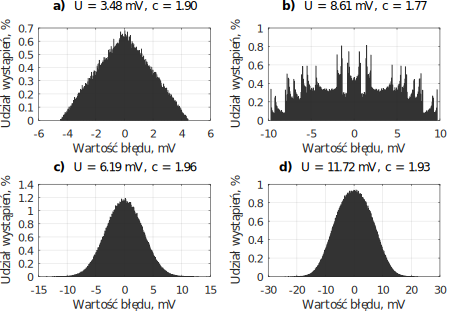
\includegraphics{obrazki/hist_part_a}
\makecaption{fig:symul_parta_hist}{Histogramy realizacji sygnałów błędów \textbf{a)}~statycznego, \textbf{b)}~dynamicznego, \textbf{c)}~losowego, \textbf{d)}~wypadkowego wielkości wyjściowej analizowanego w eksperymencie symulacyjnym przetwornika pomiarowego uzyskane metodą Monte Carlo}
\end{center}
\end{figure}

Wyznaczona na drodze eksperymentu wartość wielkości $U_{a,\Sigma}$ wyniosła~\qty{11.58}{mV}, przy czym wartość współczynnika rozszerzenia $c_{a,\Sigma}$ wyniosła~\num{1.90}. Wartość niepewności oszacowana na podstawie równania~\eqref{eq:sym_parta_uncert_value_a} jest zatem około~\qty{4.5}{\percent} większa od wartości uzyskanej na drodze eksperymentu. Należy zaznaczyć, że ta sama wartość wyznaczona za pomocą równania~\eqref{eq:sym_parta_uncert_sum} stosując współczynniki koherencji, których wartości zostały wyznaczone bez użycia zaproponowanej w pracy korekty opisanej równaniem~\eqref{eq:unc_cohercorra} wynosi~\qty{12.41}{mV}, a zatem jest ona o~\qty{7.3}{\percent} większa od wartości referencyjnej. W przypadku wartości oszacowanej na podstawie równania~\eqref{eq:sym_parta_uncert_value_b} rozbieżność jest nieco mniejsza i wynosi około~\qty{3.2}{\percent}, co dowodzi że w analizowanym przypadku spełnione zostały założenia związane z centralnym twierdzeniem granicznym, a przyjęte uproszczenia okazały się nie mieć znaczącego wpływu na wynik obliczeń. Uzyskana wartość wariancji sygnału błędu wypadkowego wielkości wyjściowej wyniosła w eksperymencie~\qty{37.1}{\micro V}, co pokrywa się z wartością wyznaczoną w równaniu~\eqref{eq:sym_parta_var_sum}. Wyznaczone w równaniach od~\eqref{eq:sym_parta_uncert_stat} do~\eqref{eq:sym_parta_factor_rand} parametry dla składowych sygnału błędu również w zadowalającym stopniu pokrywają się z uzyskanymi na drodze eksperymentu.

Zastosowana metoda szacowania wartości współczynników koherencji w celu wyznaczenia wartości wypadkowej niepewności rozszerzonej zapewnia wyniki zawyżone o kilka procent w stosunku do wartości uzyskiwanych symulacyjne. Jako że omawiane rozbieżności są niewielkie oraz ich znak jest dodatni, uzyskiwane wyniki można uznać za prawidłowe. Wadą przedstawionej metody jest jednak konieczność znajomości wartości współczynników kształtu, co powoduje, że dla rozkładów o niestandardowym kształcie jej obszar zastosowań staje się ograniczony. Zaproponowana w pracy dodatkowa korekta wartości współczynników koherencji pozwala na uzyskanie bardziej zbliżonych, do uzyskiwanych symulacyjnie, wyników obliczeń.

Wobec przedstawionych rozważań i wyników przeprowadzonego eksperymentu stwierdzić można, że zaproponowany model błędów odpowiednio opisuje związki pomiędzy kolejnymi sygnałami błędów, zachodzące w analizowanym obiekcie. Jako że kolejne fragmenty analizowanego toru pomiarowego przetwarzać będą zdefiniowane dotychczas sygnały błędów, przeprowadzony proces wyznaczania parametrów wypadkowych w przypadku grupy błędów dynamicznych oraz wyznaczanie parametrów wypadkowego błędu wielkości wyjściowej był nadmiarowy i został przeprowadzony jedynie w celu weryfikacji zaproponowanej metody obliczeń. W przypadku pozostałych grup sygnałów błędów, które cechowały się rozkładami o standardowych kształtach, wyznaczenie wypadkowych parametrów tych sygnałów pozwala na zmniejszenie liczby analizowanych sygnałów i upraszcza dalszą analizę.

\section{Analiza wzmacniacza pomiarowego}

Kolejną część toru pomiarowego stanowi wzmacniacz, którego zadaniem jest dopasowanie poziomu sygnału napięciowego $y_{a}(t)$, reprezentującego mierzoną wielkość fizyczną $s(t)$, do zakresu napięcia wejściowego $y_{b}(t)$ przetwornika analogowo-cyfrowego. Zakładane wzmocnienie układu wynosi $s_{b} = \qty{3.3}{V \per V}$, zatem w przypadku idealnym jego funkcję przetwarzania $\dot{f}_{b}(x)$ stanowi liniowa, addytywna funkcja opisana równaniem:
\begin{equation}
\dot{f}_{b} \emb{x} = s_{b} x = \num{3.3} x \label{eq:sym_partb_function},
\end{equation}
przy czym przyjęto, że nieliniowość przedstawionej charakterystyki jest pomijalnie mała i nie została rozważona w przedstawionym eksperymencie. Przyjąć można zatem założenie, że $\tilde{f}_{b}(x) \cong \dot{f}_{b}(x)$. Wobec powyższych, wielkość wyjściową analizowanego obiektu w przypadku idealnym oraz rzeczywistym opisać można jako:
\begin{gather}
\dot{y}_{b} \emb{t} = \dot{f}_{b} \emb{\dot{y}_{a} \emb{t}} = \num{3.3} \dot{y}_{a} \emb{t} \label{eq:sym_partb_out_ideal}, \\
\tilde{y}_{b} \emb{t} = \dot{y}_{b} \emb{t} + e_{b,\Sigma} \emb{t} \label{eq:sym_partb_out_real},
\end{gather}
gdzie sygnały wchodzące w skład wypadkowego sygnału błędu $e_{b,\Sigma}(t)$ opisano w dalszej części podrozdziału oraz wskazano ich parametry.

Analizowany układ wzmacniacza charakteryzuje się częstotliwością graniczną równą $f_{b,g} = \qty{650}{kHz}$, stąd zakłada się, że jego transmitancje opisać można w postaci:
\begin{equation}
\tilde{G}_{b} \emb{j\omega} = \frac{1}{1 + j \frac{\omega}{2 \pi f_{b,g}}} = \frac{1}{\frac{\omega^{2}}{4 \pi^{2} f_{b,g}^{2}} + 1} - j \frac{\omega}{2 \pi f_{b,g} \left( \frac{\omega^{2}}{4 \pi^{2} f_{b,g}^{2}} + 1 \right) } \label{eq:sym_partb_trans}.
\end{equation}
Wobec przedstawionego założenia, równania~\eqref{eq:mid_cont_amp} oraz~\eqref{eq:mid_cont_phi} można rozwinąć jako:
\begin{gather}
\tilde{K}_{b} \emb{\omega} = \sqrt{\left( \Re \left( \tilde{G}_{b} \emb{j\omega} \right) \right)^{2} + \left( \Im \left( \tilde{G}_{b} \emb{j\omega} \right) \right)^{2}} = \left( \frac{\omega^{2}}{4 \pi^{2} f_{b,g}^{2}} + 1 \right)^{-\frac{1}{2}} \label{eq:sym_partb_amp_real}, \\
\tilde{\varphi}_{b} \emb{\omega} = \arctan \left( \frac{\Im \left( \tilde{G}_{b} \emb{j\omega} \right)}{\Re \left( \tilde{G}_{b} \emb{j\omega} \right)} \right) = \arctan \left( -\frac{\omega}{2 \pi f_{b,g}} \right) \label{eq:sym_partb_phi_real},
\end{gather}
natomiast w przypadku idealnej transmitancji $\dot{G}_{b}(j\omega) = 1$ parametry te wynoszą kolejno:
\begin{gather}
\dot{K}_{b} \emb{\omega} = \sqrt{\left( \Re \left( \dot{G}_{b} \emb{j\omega} \right) \right)^{2} + \left( \Im \left( \dot{G}_{b} \emb{j\omega} \right) \right)^{2}} = \qty{1}{V \per V} \label{eq:sym_partb_amp_ideal}, \\
\dot{\varphi}_{b} \emb{\omega} = \arctan \left( \frac{\Im \left( \dot{G}_{b} \emb{j\omega} \right)}{\Re \left( \dot{G}_{b} \emb{j\omega} \right)} \right) = \qty{0}{rad} \label{eq:sym_partb_phi_ideal}.
\end{gather}

Wobec przyjętych dotychczas założeń, opisanych w równaniach~\eqref{eq:sym_partb_out_ideal}, \eqref{eq:sym_partb_amp_ideal}, \eqref{eq:sym_partb_phi_ideal} oraz założenia określającego idealny przebieg przetwarzanej wielkości wejściowej $y_{a}(t)$, opisanego równaniem~\eqref{eq:sym_parta_out_ideal_sum}, idealny przebieg wielkości wyjściowej $y_{b}(t)$ w analizowanym przypadku określa równanie:
\begin{equation}
\dot{y}_{b} \emb{t} = \sum _{i=1} ^{3} E_{b,o} \emb{\omega_{b,i}} \sin \emb{\omega_{b,i} t + \varphi_{b,i}} \label{eq:sym_partb_out_ideal_sum},
\end{equation}
natomiast parametry kolejnych harmonicznych przedstawionego sygnału opisać można dla przypadku idealnego za pomocą równań:
\begin{gather}
E_{b,o} \emb{\omega} = s_{b} \dot{K}_{b} \emb{\omega} E_{a,o} \emb{\omega} = \num{3.3} E_{a,o} \emb{\omega} \label{eq:sym_partb_amp_out_ideal}, \\
\varphi_{b,o} \emb{\omega} = \varphi_{a,o} \emb{\omega} + \dot{\varphi}_{b} \emb{\omega} = \varphi_{a,o} \emb{\omega} \label{eq:sym_partb_phi_out_ideal},
\end{gather}
gdzie $E_{b,o}(\omega)$ jest amplitudą oraz $\varphi_{b,o}(\omega)$ fazą harmonicznej sygnału wyjściowego $y_{b}(t)$ o wybranej pulsacji w przypadku idealnym, natomiast $\omega_{a,i} = \omega_{b,i}$ jest pulsacją $i$-tej harmonicznej analizowanego sygnału. Na podstawie danych zestawionych w tabeli~\ref{tab:sym_outa_params_ideal} oraz zależności od~\eqref{eq:sym_partb_out_ideal_sum} do~\eqref{eq:sym_partb_phi_out_ideal} wyznaczono parametry sygnału $y_{b}(t)$ dla przypadku idealnego i zestawiono je w tabeli~\ref{tab:sym_outb_params_ideal}.

\begin{table}[htb!]
\begin{center}
\makecaption{tab:sym_outb_params_ideal}{Parametry kolejnych harmonicznych sygnału $y_{b}(t)$ przyjęte w przeprowadzanym eksperymencie symulacyjnym dla sytuacji idealnej}
\begin{tabular}[c]{| c | c | c | c |} \hline
\textbf{$i$} & \textbf{Pulsacja $\omega_{b,i}$, rad/s} & \textbf{Amplituda $E_{b,o}(\omega_{b,i})$, V} & \textbf{Faza $\varphi_{b,o}(\omega_{b,i})$, rad} \\ \hline
1 & $1000  \cdot 2\pi$ &  \num{1.98} & $0$           \\ \hline
2 & $5000  \cdot 2\pi$ &  \num{0.99} & $\pi/8 + \pi$ \\ \hline
3 & $15000 \cdot 2\pi$ &  \num{0.33} & $\pi/6$       \\ \hline
\end{tabular}
\end{center}
\end{table}

Pierwszą omawianą grupę sygnałów błędów stanowią błędy własne, wprowadzane przez analizowany obiekt. Przyjmuje się, że temperatura otoczenia $\vartheta(t)$ wpływa na dryft zera analizowanego wzmacniacza zgodnie z zależnością opisaną równaniem:
\begin{equation}
f_{b,z} \left( \vartheta \emb{t} \right) = \frac{7}{2} \left( \vartheta \emb{t} - \qty{20}{\degreeCelsius} \right)~\unit{\frac{mV}{K}} \label{eq:sym_partb_temp_err},
\end{equation}
oraz że w czasie wykonywania pojedynczej serii pomiarowej zmiany tej temperatury będą zbliżone do zera. Błąd statyczny własny, wynikający z dryftu zera spowodowanego zmianą temperatury otoczenia, zgodnie z równaniem~\eqref{eq:out_cont_err_env_self} opisać można jako:
\begin{equation}
e_{b,sw} \emb{t} = f_{b,z} \left( \vartheta \emb{t} \right) \label{eq:sym_partb_err_sw}.
\end{equation}
Sygnał błędu dynamicznego własnego, zdefiniowany w równaniach~\eqref{eq:mid_cont_err_dyn_prop} oraz~\eqref{eq:out_cont_err_dyn_prop}, opisać można na podstawie założeń danych równaniem~\eqref{eq:sym_parta_out_ideal_sum} w postaci:
\begin{equation}
e_{b,dw} \emb{t} = \sum _{i = 1} ^{3} e_{b,dw} \emb{t,\omega_{a,i}} = \sum _{i = 1} ^{3} E_{b,ew} \emb{\omega_{b,i}} \sin \emb{\omega t + \varphi_{b,ew} \emb{\omega_{b,i}}} \label{eq:sym_partb_dyn_self_sum},
\end{equation}
natomiast kolejne harmoniczne przedstawionego sygnału mogą być opisane następująco:
\begin{equation}
\begin{split}
e_{b,dw} \emb{t,\omega} =~
& \tilde{f}_{b} \left( \tilde{K}_{b} \emb{\omega} E_{a,o} \emb{\omega} \sin \left( \omega t + \varphi_{a,o} \emb{\omega} + \tilde{\varphi}_{b} \emb{\omega} \right) \right)- \\
& \tilde{f}_{b} \left( \dot{K}_{b} \emb{\omega} E_{a,o} \emb{\omega} \sin \left( \omega t + \varphi_{a,o} \emb{\omega} + \dot{\varphi}_{b} \emb{\omega} \right) \right)
\end{split}
\label{eq:sym_partb_dyn_self_err}.
\end{equation}
Wypadkowe wartości parametrów amplitudy oraz fazy dla kolejnych harmonicznych sygnału błędu dynamicznego własnego $e_{b,dw}(t)$ zestawiono w tabeli~\ref{tab:sym_partb_params_dyn_self}, przy czym ich wartości wyznaczono analogicznie, jak w przykładzie opisanym dla poprzedniej części toru pomiarowego w równaniach od~\eqref{eq:sym_parta_dyn_self_example_harm} do~\eqref{eq:sym_parta_dyn_self_example_phi}.

Drugą grupę sygnałów błędów stanowią błędy propagowane, przenoszone z wejścia na wyjście obiektu. Sygnał błędu statycznego $e_{a,sw}(t)$ jest przenoszony na wyjście obiektu zgodnie równaniami~\eqref{eq:mid_cont_err_stat_prop} oraz~\eqref{eq:out_cont_err_stat_prop}, zatem:
\begin{equation}
e_{b,sp} \emb{t} = \tilde{f}_{b} \left( \tilde{K}_{b} \emb{0} e_{a,sw} \emb{t} \right) = \num{3.3} e_{a,sw} \emb{t} \label{eq:sym_partb_stat_prop_err}.
\end{equation}
Sygnały błędów losowych $e_{a,rw}(t)$ oraz $e_{a,rp}(t)$ wielkości wejściowej są propagowane zgodnie z zależnością~\eqref{eq:out_cont_err_rand_prop}, przy czym ze względu na niedeterministyczny opis tych sygnałów nie ma możliwości zdefiniowania postaci tych sygnałów w funkcji czasu. Stosując zaproponowany model błędów należy jedynie zdefiniować parametry tych sygnałów na wyjściu obiektu, zatem przyjmuje się, że sygnał błędu $e_{b,rp,1}(t)$ na wyjściu obiektu związany jest z sygnałem $e_{a,rw}(t)$ na jego wejściu, oraz że sygnał $e_{b,rp,2}(t)$ na wyjściu obiektu jest powiązany z sygnałem $e_{a,rp}(t)$. Na podstawie wprowadzonych założeń wypadkowy sygnał propagowanego błędu losowego wyrazić można w postaci:
\begin{equation}
e_{b,rp} \emb{t} = e_{b,rp,1} \emb{t} + e_{b,rp,2} \emb{t} \label{eq:sym_partb_rand_prop_err}.
\end{equation}
Przetwarzany przez obiekt sygnał błędu dynamicznego $e_{a,dw}(t)$ propagowany jest na wyjście zgodnie z równaniami~\eqref{eq:mid_cont_err_dyn_prop} oraz~\eqref{eq:out_cont_err_dyn_prop}, zatem wybraną harmoniczną sygnału propagowanego błędu dynamicznego $e_{b,dp}(t)$ na wyjściu tego obiektu opisuje równanie:
\begin{equation}
\begin{split}
e_{b,dp} \emb{t,\omega} =~
& \tilde{f}_{b} \left( \tilde{K}_{b} \emb{\omega} E_{a,e} \emb{\omega} \sin \left( \omega t + \varphi_{a,e} \emb{\omega} + \tilde{\varphi}_{b} \emb{\omega} \right) \right) = \\
& \num{3.3} \tilde{K}_{b} \emb{\omega} E_{a,e} \emb{\omega} \sin \left( \omega t + \varphi_{a,e} \emb{\omega} + \tilde{\varphi}_{b} \emb{\omega} \right)
\end{split}
\label{eq:sym_partb_dyn_prop_err},
\end{equation}
gdzie wypadkowe parametry kolejnych harmonicznych $e_{a,dp}(t,\omega)$ omawianego sygnału zestawiono w tabeli~\ref{tab:sym_parta_params_dyn_summary}. Wypadkowy sygnał błędu dynamicznego propagowanego $e_{b,dp}(t)$ na wyjściu analizowanego obiektu zdefiniować można zatem jako:
\begin{equation}
e_{b,dp} \emb{t} = \sum _{i = 1} ^{3} e_{b,dp} \emb{t,\omega_{a,i}} = \sum _{i = 1} ^{3} E_{b,ep} \emb{\omega_{b,i}} \sin \emb{\omega t + \varphi_{b,ep} \emb{\omega_{b,i}}} \label{eq:sym_partb_dyn_prop_sum},
\end{equation}
przy czym omówiony przypadek dotyczy założeń przyjętych w równaniu~\eqref{eq:sym_parta_dyn_self_sum}, które wynikają z założonej w równaniu~\eqref{eq:sym_in_ideal} postaci sygnału $s(t)$.

Parametry wypadkowe kolejnych harmonicznych sygnałów błędów dynamicznych własnych $e_{b,dw}(t)$ oraz propagowanych $e_{b,dp}(t)$ mogą być wyznaczone w sposób analogiczny, jak pokazano na przykładnie opisanym w równaniach od~\eqref{eq:sym_parta_dyn_self_example_sum} do~\eqref{eq:sym_parta_dyn_self_example_phi}. Wyznaczenie omawianych parametrów pozwoli na określenie wartości wariancji wymienionych sygnałów oraz wyznaczenie związanej z nimi wartości niepewności rozszerzonej. Wyznaczone zgodnie z metodą zaproponowaną w równaniach od~\eqref{eq:dyn_vect} do~\eqref{eq:dyn_vect_phi} wypadkowe amplitudy oraz fazy dla wskazanych sygnałów błędów dynamicznych przedstawiono w tabelach~\ref{tab:sym_partb_params_dyn_self} oraz~\ref{tab:sym_partb_params_dyn_prop}. Należy zauważyć, że wyznaczenie wypadkowych parametrów kolejnych harmonicznych analizowanych sygnałów nie jest konieczne z punktu widzenia stosowania zaproponowanego modelu błędów. Zabieg ten pozwala natomiast uprościć analizę poprzez redukcję liczby analizowanych sygnałów.

\begin{table}[htb!]
\begin{center}
\makecaption{tab:sym_partb_params_dyn_self}{Parametry wypadkowe kolejnych harmonicznych sygnału błędu dynamicznego własnego analizowanego w eksperymencie symulacyjnym wzmacniacza pomiarowego}
\begin{tabular}[c]{| c | c | S[table-format = 2.2] | S[table-format = +1.2] |} \hline
\textbf{$i$} & \textbf{Pulsacja $\omega_{b,i}$, rad/s} & \textbf{Amplituda $E_{b,ew}(\omega_{b,i})$, mV} & \textbf{Faza $\varphi_{b,ew}(\omega_{b,i})$, rad} \\ \hline
1 & $1000  \cdot 2\pi$  &   3.05  & -1.57  \\ \hline
2 & $5000  \cdot 2\pi$  &   7.62  &  1.96  \\ \hline
3 & $15000 \cdot 2\pi$  &   7.61  & -1.06  \\ \hline
\end{tabular}
\end{center}
\end{table}

\begin{table}[htb!]
\begin{center}
\makecaption{tab:sym_partb_params_dyn_prop}{Parametry wypadkowe kolejnych harmonicznych sygnału błędu dynamicznego propagowanego analizowanego w eksperymencie symulacyjnym wzmacniacza pomiarowego}
\begin{tabular}[c]{| c | c | S[table-format = 2.2] | S[table-format = +1.2] |} \hline
\textbf{$i$} & \textbf{Pulsacja $\omega_{b,i}$, rad/s} & \textbf{Amplituda $E_{b,ep}(\omega_{b,i})$, mV} & \textbf{Faza $\varphi_{b,ep}(\omega_{b,i})$, rad} \\ \hline
1 & $1000  \cdot 2\pi$  &   6.19  & -1.57  \\ \hline
2 & $5000  \cdot 2\pi$  &  15.47  &  1.95  \\ \hline
3 & $15000 \cdot 2\pi$  &  15.46  & -1.09  \\ \hline
\end{tabular}
\end{center}
\end{table}

Cel następnego etapu rozważań stanowi określenie parametrów wariancji oraz niepewności rozszerzonych dla opisanych dotychczas sygnałów błędów. Ze względu na liniowy charakter analizowanego obiektu, wynikający z przyjętych założeń, opisanych w równaniach~\eqref{eq:sym_partb_out_ideal} oraz~\eqref{eq:sym_partb_trans}, na wyjściu obiektu zachowane zostaną oryginalne kształty rozkładów wszystkich propagowanych sygnałów błędów~\cite{grimmett_probability, oppenheim_sns}. Wobec powyższych, znając wariancję tych sygnałów na wyjściu obiektu, wyznaczenie związanej z nimi wartości niepewności rozszerzonej odbywać się może zgodnie z zależnością~\eqref{eq:unc_sum}. Wpływ transmitancji obiektu na wartość wariancji propagowanych sygnałów błędów opisany został wcześniej równaniem~\eqref{eq:mid_cont_var_omega}, natomiast wpływ funkcji przetwarzania na tą wielkość, w przypadku liniowej funkcji przetwarzania, określa zależność~\eqref{eq:out_cont_var_sense}. Można zatem zapisać, w przypadku sygnału propagowanego błędu statycznego:
\begin{gather}
\sigma_{b,sp}^{2} = s_{b}^{2} \tilde{K}_{b}^{2} \emb{0} \sigma_{a,sw}^{2} = \num{3.3}^{2} \cdot \num{1.0}^{2} \cdot \num{3.38e-6} = \qty{36.75}{\micro V} \label{eq:sym_partb_var_stat_prop}, \\
U_{b,sp} = c_{b,sp} \sigma_{b,sp} = \qty{11.52}{mV} \label{eq:sym_partb_unc_stat_prop},
\end{gather}
przy czym $c_{b,sp} = c_{a,sw} = c_{t} = \num{1.90}$. W przypadku wypadkowego sygnału błędu dynamicznego $e_{b,d}(t)$ wariancje kolejnych składowych tego sygnału opisać można zgodnie z zależnością~\eqref{eq:dyn_var}, przy czym parametry jego harmonicznych zestawiono w tabelach~\ref{tab:sym_partb_params_dyn_self} oraz~\ref{tab:sym_partb_params_dyn_prop}. Wariancje sygnałów błędów losowych $e_{b,rp,1}(t)$ oraz $e_{b,rp,2}(t)$ można natomiast opisać w funkcji pulsacji, jako:
\begin{gather}
\sigma_{b,rp,1}^{2} \emb{\omega} = s_{b}^{2} \tilde{K}_{b} \emb{\omega} \sigma_{a,rw}^{2} \emb{\omega} \cong \qty{36.26}{\micro V} \label{eq:sym_partb_var_rand_prop_1}, \\
\sigma_{b,rp,2}^{2} \emb{\omega} = s_{b}^{2} \tilde{K}_{b} \emb{\omega} \sigma_{a,rp}^{2} \emb{\omega} = s_{a}^{2} s_{b}^{2} \tilde{K}_{a}^{2} \emb{\omega} \tilde{K}_{b} \emb{\omega} \sigma_{s,r}^{2} \emb{\omega} \cong \qty{72.64}{\micro V} \label{eq:sym_partb_var_rand_prop_2},
\end{gather}
przy czym postać przedstawionych zależności wynika z faktu, że w zakresie częstotliwości $\hat{f} \in \interval{0}{\frac{1}{2} f_{p}}$ transmitancja obiektu nie wpływa na widmo przetwarzanych sygnałów błędów losowych. Można zatem, zgodnie z zależnością~\eqref{eq:out_cont_err_rand_prop}, przyjąć założenia gdzie $e_{b,rp,1}(t) \cong \tilde{f}_{b}(e_{a,rw}(t))$ oraz $e_{b,rp,2}(t) \cong \tilde{f}_{b}(e_{a,rp}(t))$. Wartości niepewności rozszerzonych związanych z analizowanymi sygnałami opisują zatem równania:
\begin{gather}
U_{b,rp,1} = c_{b,rp,1} \sigma_{b,rp,1} = \qty{9.93}{mV} \label{eq:sym_partb_uncert_rand_prop_1}, \\
U_{b,rp,2} = c_{b,rp,2} \sigma_{b,rp,2} = \qty{16.70}{mV} \label{eq:sym_partb_uncert_rand_prop_2},
\end{gather}
gdzie $c_{b,rp,1} = c_{a,rw} = c_{u} = \num{1.65}$ oraz $c_{b,rp,2} = c_{a,rp} = c_{n} = \num{1.96}$. Należy zauważyć, że w przypadku istnienia wpływu transmitancji obiektu na widmową gęstość mocy analizowanych sygnałów, w celu wyznaczenia wartości niepewności rozszerzonej związanej z tymi sygnałami należałoby określić średnią wartość wariancji tych sygnałów dla analizowanego zakresu częstotliwości, określoną równaniem~\eqref{eq:mid_cont_var_rand}. Tabela~\ref{tab:sym_partb_params_unc_list} przedstawia budżet niepewności wielkości wyjściowej analizowanego wzmacniacza pomiarowego z uwzględnieniem podziału na sygnały błędów własnych i propagowanych, sporządzony na podstawie przedstawionych rozważań.

\begin{table}[htb!]
\begin{center}
\makecaption{tab:sym_partb_params_unc_list}{Budżet niepewności wielkości wyjściowej analizowanego w eksperymencie symulacyjnym wzmacniacza pomiarowego, gdzie ($a$)~oznacza przetwornik pomiarowy oraz ($b$)~oznacza wzmacniacz pomiarowy}
\begin{tabular}[c]{| c | c | S[table-format = 2.2] | S[table-format = 3.2] | c | c |} \hline
\textbf{Lp.} & \textbf{Symbol} & \textbf{$U$, mV} & \textbf{$\sigma^{2}$, \micro V} & \textbf{Rozkład} & \textbf{Źródło błędu} \\ \hline
1  & ${b,sp}$       & 11.52 &  36.75  & trójkątny                    & dryft temperatury ($a$)                    \\ \hline
2  & ${b,sw}$       & 8.15  &  18.38  & trójkątny                    & dryft temperatury ($b$)                    \\ \hline
3  & ${b,rp,1}$     & 9.93  &  36.26  & jednostajny                  & nieliniowość obiektu ($a$)                 \\ \hline
4  & ${b,rp,2}$     & 16.70 &  72.64  & normalny                     & szum wielkości wejściowej                  \\ \hline
5  & ${b,dp,1}$     & 6.21  &  19.14  & \multirow{6}{*}{dwumodalny}  & \multirow{3}{*}{transmitancja ($a$)}       \\ \cline{1-4}
6  & ${b,dp,2}$     & 15.53 &  119.62 &                              &                                            \\ \cline{1-4}
7  & ${b,dp,3}$     & 15.52 &  119.44 &                              &                                            \\ \cline{1-4} \cline{6-6}
8  & ${b,dw,1}$     & 3.06  &  4.64   &                              & \multirow{3}{*}{transmitancja ($b$)}       \\ \cline{1-4}
9  & ${b,dw,2}$     & 7.65  &  29.00  &                              &                                            \\ \cline{1-4}
10 & ${b,dw,3}$     & 7.65  &  28.99  &                              &                                            \\ \hline
\end{tabular}
\end{center}
\end{table}

Dla źródeł błędów wymienionych w budżecie niepewności, zestawionym w tabeli~\ref{tab:sym_partb_params_unc_list}, konieczne jest określenie wzajemnych korelacji pomiędzy sygnałami błędów. Należy zauważyć, że składowe związane z dryftem temperaturowym przetwornika pomiarowego oraz dryftem temperaturowym wzmacniacza zależą od tej samej wielkości fizycznej -- temperatury otoczenia. Jako że wymienione sygnały błędów nie zależą od żadnej innej wielkości, a dodatkowo równania~\eqref{eq:sym_parta_stat_err} oraz~\eqref{eq:sym_partb_temp_err} cechują się dodatnią czułością względem tej wielkości, można założyć pełną dodatnią korelacje analizowanych sygnałów błędów, zatem $r_{b,sw,b,sp} = r_{b,sp,b,sw} = 1$. W przypadku kolejnych harmonicznych sygnałów błędów dynamicznych wartość współczynnika korelacji tych składowych może być obliczona zgodnie z równaniem~\eqref{eq:dyn_corr}. Można zauważyć, że wartość tego współczynnika dla par składowych o różnej pulsacji każdorazowo wyniesie zero. W przypadku par harmonicznych sygnałów błędów dynamicznych o identycznej pulsacji, na podstawie danych zawartych w tabelach~\ref{tab:sym_partb_params_dyn_self} oraz~\ref{tab:sym_partb_params_dyn_prop}, zauważyć można, że współczynnik korelacji zbliżony będzie od jedności, ze względu na zbliżoną do zera różnicę w fazach tych sygnałów. W przypadku pozostałych par sygnałów wartości współczynników korelacji będą zerowe.

Biorąc pod uwagę przedstawione informacje na temat istniejących korelacji pomiędzy analizowanymi sygnałami błędów należy zauważyć, że zastosowanie opisanej równaniem~\eqref{eq:unc_matrix} metody wyznaczania wartości wypadkowej niepewności rozszerzonej nie będzie możliwe dla wartości współczynników koherencji wyznaczanych zgodnie z równaniem~\eqref{eq:unc_coher}. Ograniczenie to wynika z faktu, że opisane w równaniach~\eqref{eq:unc_cohercorra} oraz~\eqref{eq:unc_cohercorrb} korekty, a także wartości współczynników kształtu, wyznaczane zgodnie z równaniem~\eqref{eq:unc_shapertwo}, nie są odpowiednie dla sytuacji, gdzie pomiędzy analizowanymi sygnałami występuje korelacja. Proponuje się zatem, w celu umożliwienia zastosowania przedstawionej metody analizy, wyznaczenie wypadkowych parametrów wariancji i niepewności rozszerzonych dla skorelowanych grup sygnałów. Jako że zaproponowana operacja prowadzi do redukcji liczby analizowanych sygnałów błędów poprzez wprowadzenie wypadkowych sygnałów dla analizowanych grup, proponuje się równolegle określić budżet niepewności dla rozważanego fragmentu toru pomiarowego, który zorientowany będzie pod kątem charakteru realizacji wymienionych w nim sygnałów.

Na podstawie zależności od~\eqref{eq:sym_partb_err_sw} do~\eqref{eq:sym_partb_dyn_prop_sum}, zgodnie z równaniem~\eqref{eq:out_cont_err_sum_all}, opisać można wprowadzony w równaniu~\eqref{eq:sym_partb_out_real} wypadkowy sygnał błędu $e_{b,\Sigma}(t)$ wielkości wyjściowej analizowanego wzmacniacza pomiarowego następującym równaniem:
\begin{equation}
e_{b,\Sigma} \emb{t} = e_{b,s} \emb{t} + e_{b,d} \emb{t} + e_{b,r} \emb{t} \label{eq:sym_partb_error_sum},
\end{equation}
w którym kolejne składniki przedstawionego sygnału zdefiniowane są w postaci:
\begin{gather}
e_{b,s} \emb{t} = e_{b,sw} \emb{t} + e_{b,sp} \emb{t} \label{eq:sym_partb_error_stat}, \\
e_{b,d} \emb{t} = e_{b,dw} \emb{t} + e_{b,dp} \emb{t} \label{eq:sym_partb_error_dyn}, \\
e_{b,r} \emb{t} = e_{b,rp} \emb{t} \label{eq:sym_partb_error_rand},
\end{gather}
gdzie $e_{b,s}(t)$ jest wypadkowym sygnałem błędu statycznego, $e_{b,d}(t)$ dynamicznego oraz $e_{b,r}(t)$ losowego. Wypadkowy sygnał błędu dynamicznego opisać można w postaci:
\begin{equation}
e_{b,d} \emb{t} = \sum _{i=1} ^{3} E_{b,e} \emb{\omega_{b,i}} \sin \emb{\omega t + \varphi_{b,e} \emb{\omega_{b,i}}} \label{sym_partb_error_dyn_sum},
\end{equation}
przy czym $E_{b,e}(\omega)$ jest wypadkową amplitudą, natomiast $\varphi_{b,e}(\omega)$ wypadkową fazą harmonicznej tego sygnału o wskazanej pulsacji. Wyznaczenie wypadkowych wartości amplitudy oraz fazy dla kolejnych harmonicznych sygnału błędu dynamicznego $e_{b,d}(t)$ przebiega zgodnie z metodą zaproponowaną w równaniach od~\eqref{eq:dyn_vect} do~\eqref{eq:dyn_vect_phi}, przy czym kolejne składniki tych harmonicznych wymienione zostały w równaniach~\eqref{eq:sym_partb_dyn_self_err} oraz~\eqref{eq:sym_partb_dyn_prop_err}. Przedstawiony proces odbywać się może również z wykorzystaniem parametrów opisanych w tabelach~\ref{tab:sym_partb_params_dyn_self} oraz~\ref{tab:sym_partb_params_dyn_prop}, przy czym niezależnie od stosowanej metody uzyskuje się identyczne wyniki obliczeń. Wartości omawianych parametrów, wyznaczone zgodnie z przedstawionymi zależnościami, zestawiono w tabeli~\ref{tab:sym_partb_params_dyn_summary}.

\begin{table}[htb!]
\begin{center}
\makecaption{tab:sym_partb_params_dyn_summary}{Parametry wypadkowe kolejnych harmonicznych sygnału błędu dynamicznego analizowanego w eksperymencie symulacyjnym wzmacniacza pomiarowego}
\begin{tabular}[c]{| c | c | S[table-format = 2.2] | S[table-format = +1.2] |} \hline
\textbf{$i$} & \textbf{Pulsacja $\omega_{b,i}$, rad/s} & \textbf{Amplituda $E_{b,e}(\omega_{b,i})$, mV} & \textbf{Faza $\varphi_{b,e}(\omega_{b,i})$, rad} \\ \hline
1 & $1000  \cdot 2\pi$  &   9.23  & -1.57  \\ \hline
2 & $5000  \cdot 2\pi$  &  23.08  &  1.96  \\ \hline
3 & $15000 \cdot 2\pi$  &  23.07  & -1.07  \\ \hline
\end{tabular}
\end{center}
\end{table}

Parametry wypadkowego sygnału błędu statycznego $e_{b,s}(t)$, zdefiniowanego zależnością~\eqref{eq:sym_partb_error_stat}, opisują równania~\eqref{eq:var_matrix} oraz~\eqref{eq:unc_matrix}, przy czym:
\begin{gather}
\begin{split}
\sigma_{b,s}^{2} = ~ &
\begin{bmatrix}
\sigma_{b,sw} \\ \sigma_{b,sp}
\end{bmatrix}^{T}
\begin{bmatrix}
1 & r_{b,sw,sp} \\
r_{b,sp,sw} & 1
\end{bmatrix}
\begin{bmatrix}
\sigma_{b,sw} \\ \sigma_{b,sp}
\end{bmatrix} = \\ &
\begin{bmatrix}
\num{6.06e-3} \\ \num{4.29e-3}
\end{bmatrix}^{T}
\begin{bmatrix}
1 & 1 \\
1 & 1
\end{bmatrix}
\begin{bmatrix}
\num{6.06e-3} \\ \num{4.29e-3}
\end{bmatrix} = \qty{107.12}{\micro V}
\end{split}
\label{eq:sym_partb_stat_var}, \\
\begin{split}
U_{b,s} = ~ & \sqrt{
\begin{bmatrix}
U_{b,sw} \\ U_{b,sp}
\end{bmatrix}^{T}
\begin{bmatrix}
1 & h_{b,sw,sp} \\
h_{b,sp,sw} & 1
\end{bmatrix}
\begin{bmatrix}
U_{b,sw} \\ U_{b,sp}
\end{bmatrix}} = \\ & \sqrt{
\begin{bmatrix}
\num{11.52e-3} \\ \num{8.15e-3}
\end{bmatrix}^{T}
\begin{bmatrix}
1 & 1 \\
1 & 1
\end{bmatrix}
\begin{bmatrix}
\num{11.52e-3} \\ \num{8.15e-3}
\end{bmatrix}} = \qty{19.67}{mV}
\end{split}
\label{eq:sym_partb_stat_uncert},
\end{gather}
gdzie współczynniki koherencji $h_{b,sw,sp} = h_{b,sp,sw} = 1$ w przypadku pełnej dodatniej korelacji, jaka ma miejsce w omawianym przypadku. W przypadku sygnałów błędów losowych propagowanych korelacja nie występuje, a zatem wariancja wypadkowego sygnału błędu losowego $e_{b,r}(t)$ jest wyznaczana zgodnie z zależnością~\eqref{eq:var_sum}, zatem:
\begin{equation}
\sigma_{b,r}^{2} = \sigma_{b,rp,1}^{2} + \sigma_{b,rp,2}^{2} = \qty{108.90}{\micro V} \label{eq:sym_partb_rand_var}.
\end{equation}
Wypadkową niepewność rozszerzoną w analizowanym przypadku wyznaczyć można zgodnie z równaniem~\eqref{eq:unc_matrix}, a zatem jej wartość wynosi:
\begin{gather}
\begin{split}
U_{a,r} = ~ & \sqrt{
\begin{bmatrix}
U_{a,rp,1} \\ U_{b,rp,2}
\end{bmatrix}^{T}
\begin{bmatrix}
1            & h_{a,rp,1,2} \\
h_{a,rp,2,1} & 1
\end{bmatrix}
\begin{bmatrix}
U_{a,rp,1} \\ U_{b,rp,2}
\end{bmatrix}} = ~ \\ & \sqrt{
\begin{bmatrix}
\num{9.93e-3} \\ \num{16.70e-3}
\end{bmatrix}^{T}
\begin{bmatrix}
\num{1.000} & \num{0.120} \\
\num{0.120} & \num{1.000}
\end{bmatrix}
\begin{bmatrix}
\num{9.93e-3} \\ \num{16.70e-3}
\end{bmatrix}} = \qty{20.43}{mV}
\end{split}
\label{eq:sym_partb_rand_uncert}, \\
h_{b,rp,1,2} = s_{u,n} \sqrt{\frac{\num{9.93e-3}}{\num{16.70e-3}}} \left( \frac{\num{98.60e-6} + \num{278.89e-6}}{\num{377.49e-6}} \right) = \num{0.120} \label{eq:sym_partb_coher_rp_1_2}.
\end{gather}
Dla kolejnych harmonicznych wypadkowego sygnału błędu dynamicznego, zestawionych w tabeli~\ref{tab:sym_partb_params_dyn_summary}, wartość wariancji wyznaczana jest zgodnie z równaniem~\eqref{eq:dyn_var}, natomiast wartość niepewności rozszerzonej wyznacza się na podstawie wzoru~\eqref{eq:unc_sum} dla $c_{d} = \num{1.41}$.

Stosując zależności przedstawione w równaniach od~\eqref{eq:sym_partb_stat_var} do~\eqref{eq:sym_partb_rand_uncert} oraz dane zawarte w tabeli~\ref{tab:sym_partb_params_dyn_summary} sporządzono budżet niepewności uwzględniający podział na zaproponowane w pracy kategorie sygnałów błędów, który zestawiono w tabeli~\ref{tab:sym_partb_params_unc_sum}. Ze względu na konieczność przeprowadzania dalszej analizy w dziedzinie pulsacji, nie wyznaczano wypadkowych parametrów błędu dynamicznego $e_{b,d}(t)$ oraz parametrów wypadkowego sygnału błędu $e_{b,\Sigma}(t)$ wielkości wyjściowej $y_{b}(t)$.

\begin{table}[htb!]
\begin{center}
\makecaption{tab:sym_partb_params_unc_sum}{Budżet niepewności wielkości wyjściowej analizowanego w eksperymencie symulacyjnym wzmacniacza pomiarowego uwzględniający wypadkowe parametry sygnałów błędów}
\begin{tabular}[c]{| c | c | S[table-format = 2.2] | S[table-format = 3.2] | c | c |} \hline
\textbf{Lp.} & \textbf{Symbol} & \textbf{$U$, mV} & \textbf{$\sigma^{2}$, \micro V} & \textbf{Rozkład} & \textbf{Źródło błędu} \\ \hline
1 & ${b,s}$        & 19.67 &  107.12 & trójkątny                    & wypadkowy dryft temperatury                \\ \hline
2 & ${b,r}$        & 20.43 &  108.90 & normalny                     & szum i nieliniowość obiektu                \\ \hline
3 & ${b,d,1}$      & 9.20  &  42.60  & \multirow{3}{*}{dwumodalny}  & \multirow{3}{*}{wypadkowa transmitancja}   \\ \cline{1-4}
4 & ${b,d,2}$      & 23.01 &  266.34 &                              &                                            \\ \cline{1-4}
5 & ${b,d,3}$      & 23.00 &  266.11 &                              &                                            \\ \hline
\end{tabular}
\end{center}
\end{table}

W celu weryfikacji poprawności założeń zastosowanego modelu błędów oraz przeprowadzonych obliczeń wykonano eksperyment metodą Monte Carlo, polegający na wyznaczeniu~\num{100000} razy wartości realizacji wielkości wyjściowej $y_{b}(t)$ analizowanego obiektu. Podczas eksperymentu fazę sygnału wejściowego $s(t+t_{0})$ losowano z przedziału $\hat{t}_{0} \in \interval{-\frac{1}{f_{1}}}{\frac{1}{f_{1}}}$ o jednakowym prawdopodobieństwie wystąpienia każdej z wartości. Uzyskiwaną wartość realizacji wielkości wyjściowej porównywano z wartością otrzymaną dla fragmentu toru pomiarowego w przypadku idealnym (tj. z taką, dla której nie występowały żadne źródła błędów), a następnie na podstawie równania~\eqref{eq:sym_partb_out_real} wyznaczano realizację błędu wielkości wyjściowej $y_{b}(t)$. Na podstawie uzyskanych wartości realizacji sygnału błędu, zgodnie z równaniem~\eqref{eq:unc_summation}, określono wartość niepewności rozszerzonej związanej z tym sygnałem. Eksperyment wykonano uwzględniając wszystkie źródła błędów oraz uwzględniając tylko źródła związane z sygnałami błędu statycznego $e_{b,s}(t)$, dynamicznego $e_{b,d}(t)$ oraz losowego $e_{b,r}(t)$. Uzyskane na drodze eksperymentu histogramy przedstawiono na rysunku~\ref{fig:symul_partb_hist}.

\begin{figure}[htb!]
\begin{center}
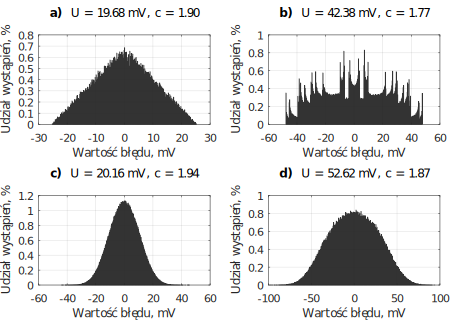
\includegraphics{obrazki/hist_part_b}
\makecaption{fig:symul_partb_hist}{Histogramy realizacji sygnałów błędów \textbf{a)}~statycznego, \textbf{b)}~dynamicznego, \textbf{c)}~losowego, \textbf{d)}~wypadkowego wielkości wyjściowej analizowanego w eksperymencie symulacyjnym wzmacniacza pomiarowego uzyskane metodą Monte Carlo}
\end{center}
\end{figure}

Analizując wyniki eksperymentu zauważyć można, że uzyskane wartości dla sygnałów błędów losowego oraz statycznego są zbliżone do tych przedstawionych w tabeli~\ref{tab:sym_partb_params_unc_sum}. Pozwala to zakładać, że podobnie jak w przypadku analizy właściwości przetwornika pomiarowego, przyjęty model błędów oraz stosowane zależności poprawnie określają związki pomiędzy wskazanymi sygnałami błędów i umożliwiają poprawne oszacowanie ich parametrów. Na dotychczasowym etapie przeprowadzonej analizy nie wyznaczano wypadkowych parametrów sygnału błędu dynamicznego $e_{b,d}(t)$ oraz sygnału błędu wypadkowego $e_{b,\Sigma}(t)$ -- dane te, jak pokazano na obecnym przykładzie, nie są niezbędne podczas analizy kolejnych fragmentów toru pomiarowego, przy czym zostały one wyznaczone w ramach analizy poprzedniej części tego toru w celu weryfikacji zaproponowanej metody obliczeń.

\section{Analiza przetwornika analogowo-cyfrowego}

Kolejnym elementem wchodzącym w skład analizowanego toru pomiarowego jest przetwornik analogowo-cyfrowy. W eksperymencie zakłada się, że element ten jest realizowany przy użyciu~\qty{8}{\bitOwego} przetwornika wagowego, którego dopuszczalna wartość napięcia wejściowego zawiera się w przedziale $\hat{y}_{b}(t) \in \interval{-3}{3}~\unit{V}$. Liczba dostępnych wartości realizacji wielkości wyjściowej $x_{c}(i)$ tego przetwornika wynosi zatem $N_{q} = 2^{8} = 256$, natomiast wartość kwantu jest równa $q = \frac{3 - (-3)}{256} = \qty{23.44}{mV}$.

Zakładając, że wielkością wyjściową $x_{c}(i)$ analizowanego przetwornika będzie dyskretna reprezentacja wielkości wejściowej $y_{b}(t)$ wyrażona w jednostce tej wielkości, na podstawie równania~\eqref{eq:adc_qerror} oraz równań od~\eqref{eq:adc_out_ideal} do~\eqref{eq:adc_out_error} zapisać można:
\begin{gather}
\dot{x}_{c} \emb{i} = \dot{y}_{b} \emb{iT_{p}} \label{eq:sym_partc_out_ideal}, \\
\tilde{x}_{c} \emb{i} = \tilde{y}_{b} \emb{iT_{p}} + e_{c,AC,q} \left( \tilde{y}_{b} \emb{iT_{p}} \right) = \dot{x}_{c} \emb{i} + e_{c,\Sigma} \emb{i} \label{eq:sym_partc_out_real}, \\
e_{c,\Sigma} \emb{i} \cong e_{b,\Sigma} \emb{iT_{p}} + e_{c,rw,q} \emb{i} \label{eq:sym_partc_error_sum},
\end{gather}
gdzie $T_{p} = \frac{1}{f_{p}} = \qty{20.8(3)}{\micro s}$ jest okresem próbkowania. Na podstawie zależności danych równaniami od~\eqref{eq:adc_function} do~\eqref{eq:adc_qerrrange} zapisać można nierówność określającą przedział, w jakim znajdować się mogą wartości realizacji sygnału błędu kwantowania $e_{c,rw,q}(i)$ jako:
\begin{equation}
\qty{-11.72}{mV} \le \hat{e}_{c,rw,q} \emb{i} \le \qty{11.72}{mV} \label{eq:sym_partc_error_quant}.
\end{equation}
Analizując równanie~\eqref{eq:sym_partc_out_real} zauważyć można, że rzeczywiste wartości realizacji błędu kwantowania $e_{AC,c,q}(x)$ zależne są od wartości realizacji wielkości wejściowej $y_{b}(t)$. Jednakże, jak wykazano w pracach~\cite{sienkowski_kwant, sienkowski_adc}, zależność tą można pominąć. Przy założeniu, że uzyskanie na wejściu przetwornika dowolnej wartości z zakresu wartości wielkości wejściowej jest jednakowo prawdopodobne oraz że podczas pomiaru wielkość ta będzie się zmieniać, błąd kwantowania oznaczony jako $e_{c,rw,q}(i)$ rozpatrywać można w kategoriach probabilistycznych, jako losową realizację wielkości z zakresu opisanego nierównością~\eqref{eq:sym_partc_error_quant} o rozkładzie jednostajnym~\cite{jakubiec_system}. Podejście to umożliwia zastosowanie zaproponowanego w pracy modelu błędów, gdzie analiza zakładająca funkcję przetwarzania daną w postaci równania~\eqref{eq:adc_output} byłaby niemożliwa. Wariancja $\sigma_{c,rw,q}^{2}$ oraz niepewność rozszerzona $U_{c,rw,q}$, związane z sygnałem $e_{c,rw,q}(i)$, wynoszą:
\begin{gather}
\sigma_{c,rw,q}^{2} = \frac{ q^{2}}{12} = \frac{\emb{\num{23.44e-3}}^{2} }{12} = \qty{45.78}{\micro V} \label{eq:sym_partc_var_quant}, \\
U_{c,rw,q} = c_{u} \sigma_{c,rw,q} = \num{1.65} \cdot \num{6.77e-3} = \qty{11.16}{mV} \label{eq:sym_partc_uncert_quant},
\end{gather}
gdzie zgodnie z założeniami opisanymi w~\cite{gray_quantization, widrow_quantization} przyjmuje się model błędu kwantowania zbliżony do modelu addytywnego szumu o stałej widmowej gęstości mocy i jednakowym prawdopodobieństwie uzyskania każdej z możliwych realizacji tego błędu.

Aby zweryfikować poprawność przedstawionych zależności przeprowadzono eksperyment stosując metodę Monte Carlo. W ramach eksperymentu~\num{100000} razy wyznaczono wartość realizacji wielkości wyjściowej analizowanego obiektu, a następnie porównano ją z wartością idealną, uzyskaną dla fragmentu toru pomiarowego w którym nie występowały żadne źródła błędów. Działanie analizowanego przetwornika opisane było równaniem zgodnym z zależnością~\eqref{eq:adc_output}. Na podstawie uzyskanych zgodnie z równaniem~\eqref{eq:sym_partc_out_real} wartości realizacji sygnału błędu wyznaczono wariancję tego sygnału oraz niepewność rozszerzoną na podstawie równania~\eqref{eq:unc_summation}. Identyczny eksperyment przeprowadzono ponownie z tą różnicą, że jako jedyne źródło błędów uwzględniono w nim obecność procesu kwantowania w celu oszacowania parametrów sygnału błędu kwantowania. Rysunek~\ref{fig:symul_partc_hist} przedstawia uzyskane na drodze eksperymentu histogramy.

\begin{figure}[htb!]
\begin{center}
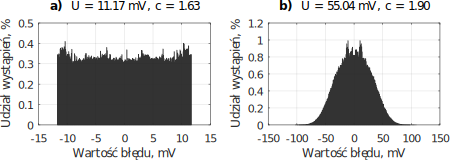
\includegraphics{obrazki/hist_part_c}
\makecaption{fig:symul_partc_hist}{Histogramy realizacji sygnałów błędów \textbf{a)}~kwantowania, \textbf{b)}~wypadkowego wielkości wyjściowej analizowanego w eksperymencie symulacyjnym przetwornika analogowo-cyfrowego uzyskane metodą Monte Carlo}
\end{center}
\end{figure}

Przedstawione na rysunkach~\ref{fig:symul_partb_hist} oraz~\ref{fig:symul_partc_hist} histogramy pozwalają stwierdzić, że przyjęte dla modelu błędu kwantowania założenia są poprawne. W poprzednim eksperymencie wartość wariancji $\sigma_{b,\Sigma}^{2}$ wypadkowego sygnału błędu wielkości wejściowej przetwornika analogowo-cyfrowego wyniosła~\qty{788.18}{\micro V}. W bieżącym eksperymencie wartość wariancji $\sigma_{c,\Sigma}^{2}$ wypadkowego sygnału błędu wielkości wyjściowej tego przetwornika wyniosła~\qty{835.18}{\micro V}. Oszacowana wartość wariancji $\sigma_{c,AC,q}^{2}$ sygnału błędu kwantowania dla założenia $\tilde{y}_{b}(i) = \dot{y}_{b}(i)$ wyniosła~\qty{46.88}{\micro V}, a związana z nią niepewność rozszerzona wyniosła~\qty{11.16}{mV}. Uzyskane wartości pokrywają się z tymi wyznaczonymi na podstawie równań~\eqref{eq:sym_partc_var_quant} oraz~\eqref{eq:sym_partc_uncert_quant} dla modelu błędu kwantowania $e_{c,rw,q}(i)$. Korelację pomiędzy wypadkowym sygnałem błędu $e_{c,\Sigma}(i)$ wielkości wejściowej analizowanego przetwornika oraz rzeczywistym sygnałem błędu kwantowania $e_{c,AC,q}(x)$ określić można na podstawie równania~\eqref{eq:var_corr}, przy czym jej wartość wynosi:
\begin{equation}
r_{c,AC,q;b,\Sigma} = \frac{\sigma_{c,\Sigma}^{2} - \sigma_{c,AC,q}^{2} - \sigma_{b,\Sigma}^{2}}{2 \sigma_{c,AC,q} \sigma_{b,\Sigma}} = \num{7.8e-4} \label{eq:sym_partc_corr}.
\end{equation}
Jako że omawiana korelacja jest pomijalnie mała, zasadne jest przyjęcie założenia braku korelacji sygnałów $e_{c,rw,q}(i)$ oraz $e_{b,\Sigma}(t)$, wobec którego $r_{c,rw,q;b,\Sigma} = 0$. Zgodnie z założeniami~\eqref{eq:adc_varout} oraz~\eqref{eq:adc_errout} przedstawić można zatem następujące relacje:
\begin{gather}
e_{c} \emb{i} \cong e_{b} \emb{iT_{p}} \label{eq:sym_partc_err_prop}, \\
\sigma_{c}^{2} \emb{\omega} \cong \sigma_{b}^{2} \emb{\omega} \label{eq:sym_partc_var_prop},
\end{gather}
opisujące sygnały błędów na wyjściu analizowanego obiektu i związane z nimi wariancje. Na podstawie przedstawionych dotychczas zależności oraz danych zawartych w tabeli~\ref{tab:sym_partb_params_unc_list} sporządzono budżet niepewności wielkości wyjściowej $x_{c}(i)$ analizowanego przetwornika analogowo-cyfrowego, który zestawiono w tabeli~\ref{tab:sym_partc_params_unc_list}.

\begin{table}[htb!]
\begin{center}
\makecaption{tab:sym_partc_params_unc_list}{Budżet niepewności wielkości wyjściowej analizowanego w eksperymencie symulacyjnym przetwornika analogowo-cyfrowego, gdzie ($a$) oznacza przetwornik pomiarowy, ($b$) oznacza wzmacniacz pomiarowy oraz ($c$) oznacza przetwornik analogowo-cyfrowy}
\begin{tabular}[c]{| c | c | S[table-format = 2.2] | S[table-format = 3.2] | c | c |} \hline
\textbf{Lp.} & \textbf{Symbol} & \textbf{$U$, mV} & \textbf{$\sigma^{2}$, \micro V} & \textbf{Rozkład} & \textbf{Źródło błędu} \\ \hline
1  & ${c,rw,q}$     & 11.16 &  45.78  & jednostajny                  & proces kwantowania ($c$)                   \\ \hline
2  & ${c,sp,1}$     & 11.52 &  36.75  & trójkątny                    & dryft temperatury ($a$)                    \\ \hline
3  & ${c,sp,2}$     & 8.15  &  18.38  & trójkątny                    & dryft temperatury ($b$)                    \\ \hline
4  & ${c,rp,1}$     & 9.93  &  36.26  & jednostajny                  & nieliniowość obiektu ($a$)                 \\ \hline
5  & ${c,rp,2}$     & 16.70 &  72.64  & normalny                     & szum wielkości wejściowej                  \\ \hline
6  & ${c,dp,a,1}$   & 6.21  &  19.14  & \multirow{6}{*}{dwumodalny}  & \multirow{3}{*}{transmitancja ($a$)}       \\ \cline{1-4}
7  & ${c,dp,a,2}$   & 15.53 &  119.62 &                              &                                            \\ \cline{1-4}
8  & ${c,dp,a,3}$   & 15.52 &  119.44 &                              &                                            \\ \cline{1-4} \cline{6-6}
9  & ${c,dp,b,1}$   & 3.06  &  4.64   &                              & \multirow{3}{*}{transmitancja ($b$)}       \\ \cline{1-4}
10 & ${c,dp,b,2}$   & 7.65  &  29.00  &                              &                                            \\ \cline{1-4}
11 & ${c,dp,b,3}$   & 7.65  &  28.99  &                              &                                            \\ \hline
\end{tabular}
\end{center}
\end{table}

Przedstawiony w tabeli~\ref{tab:sym_partc_params_unc_list} budżet niepewności dobrze obrazuje źródła sygnałów błędów występujące w analizowanym torze pomiarowym oraz jednoznacznie wskazuje ich parametry. Na dalszym etapie analizy stosowanie przedstawionego zestawienia jest jednak kłopotliwe, ponieważ wiąże się z koniecznością analizy każdego ze wskazanych sygnałów błędów z osobna. Ze względu na fakt, że proponowany w pracy model błędów dotyczący kolejnego fragmentu toru pomiarowego, jakim jest algorytm transformacji falkowej, wymaga jedynie określenia parametrów wypadkowych sygnałów błędów statycznego i losowego oraz wypadkowych parametrów kolejnych harmonicznych sygnału błędu dynamicznego, proponuje się sporządzenie budżetu niepewności uwzględniającego opisywany podział, podobnie jak to miało miejsce w przypadku poprzedniego elementu analizowanego toru pomiarowego.

Parametry opisujące wypadkowy sygnał błędu losowego wyznaczyć można zgodnie z równaniami~\eqref{eq:var_sum} oraz~\eqref{eq:unc_matrix}, które w obecnym przypadku przyjmują postać:
\begin{gather}
\sigma_{c,r}^{2} = \sigma_{c,rp,1}^{2} + \sigma_{c,rp,2}^{2} + \sigma_{c,rw,q}^{2} = \sigma_{b,rp,1}^{2} + \sigma_{b,rp,2}^{2} + \sigma_{c,rw,q}^{2} = \qty{154.68}{\micro V} \label{eq:sym_partc_rand_var}, \\
\begin{split}
U_{c,r} = ~ & \sqrt{
\begin{bmatrix}
U_{c,rp,1} \\ U_{c,rp,2} \\ U_{c,rw,q}
\end{bmatrix}^{T}
\begin{bmatrix}
1               & h_{c,rp,1,2}    & h_{c,rp,1,rw,q} \\
h_{c,rp,2,1}    & 1               & h_{c,rp,2,rw,q} \\
h_{c,rw,q,rp,1} & h_{c,rw,q,rp,2} & 1
\end{bmatrix}
\begin{bmatrix}
U_{c,rp,1} \\ U_{c,rp,2} \\ U_{c,rw,q}
\end{bmatrix}} = ~ \\ & \sqrt{
\begin{bmatrix}
\num{9.93e-3} \\ \num{16.70e-3} \\ \num{11.16e-3}
\end{bmatrix}^{T}
\begin{bmatrix}
\num{1.000} & \num{0.091} & \num{0.141} \\
\num{0.091} & \num{1.000} & \num{0.103} \\
\num{0.141} & \num{0.103} & \num{1.000}
\end{bmatrix}
\begin{bmatrix}
\num{9.93e-3} \\ \num{16.70e-3} \\ \num{11.16e-3}
\end{bmatrix}} = \qty{24.53}{mV}
\end{split}
\label{eq:sym_partc_rand_uncert}, \\
h_{c,rp,1,2} = s_{u,n} \sqrt{\frac{\num{9.93e-3}}{\num{16.70e-3}}} \left( \frac{\num{98.60e-6} + \num{278.89e-6}}{\num{502.04e-6}} \right) = \num{0.091} \label{eq:sym_partc_coher_rp_1_2}, \\
h_{c,rw,q,rp,1} = s_{u,u} \sqrt{\frac{\num{9.93e-3}}{\num{11.16e-3}}} \left( \frac{\num{98.60e-6} + \num{124.55e-6}}{\num{502.04e-6}} \right) = \num{0.141} \label{eq:sym_partc_coher_q_rp_1}, \\
h_{c,rw,q,rp,2} = s_{u,n} \sqrt{\frac{\num{11.16e-3}}{\num{16.70e-3}}} \left( \frac{\num{124.55e-6} + \num{278.89e-6}}{\num{502.04e-6}} \right) = \num{0.103} \label{eq:sym_partc_coher_q_rp_2}, \\
c_{c,r} = \frac{U_{c,r}}{\sigma_{c,r}} = \frac{\num{24.53e-3}}{\num{12.44e-3}} = \num{1.97} \label{eq:sym_partc_rand_factor}.
\end{gather}

Na podstawie wyznaczonej w równaniu~\eqref{eq:sym_partc_rand_factor} wartości współczynnika rozszerzenia oraz ze względu na spełnienie w analizowanym przypadku warunków centralnego twierdzenia granicznego, zakładać można normalny rozkład wypadkowego sygnału błędu losowego. Biorąc pod uwagę przedstawione dotychczas założenia, wyniki zawarte w tabelach~\ref{tab:sym_partb_params_unc_sum} oraz~\ref{tab:sym_partc_params_unc_list}, jak również wyniki obliczeń przedstawionych w równaniach~\eqref{eq:sym_partc_rand_var} oraz~\eqref{eq:sym_partc_rand_uncert}, sporządzono budżet niepewności z uwzględnieniem omawianego wcześniej podziału, który zestawiono w tabeli~\ref{tab:sym_partc_params_unc_sum}.

\begin{table}[htb!]
\begin{center}
\makecaption{tab:sym_partc_params_unc_sum}{Budżet niepewności wielkości wyjściowej analizowanego w eksperymencie symulacyjnym przetwornika analogowo-cyfrowego z uwzględnieniem podziału na wypadkowe sygnały błędów statycznych, dynamicznych oraz losowych}
\begin{tabular}[c]{| c | c | S[table-format = 2.2] | S[table-format = 3.2] | c | c |} \hline
\textbf{Lp.} & \textbf{Symbol} & \textbf{$U$, mV} & \textbf{$\sigma^{2}$, \micro V} & \textbf{Rozkład} & \textbf{Źródło błędu} \\ \hline
1 & ${c,s}$        & 19.67 &  107.12 & trójkątny                    & wypadkowy dryft temperatury                \\ \hline
2 & ${c,r}$        & 24.53 &  154.68 & normalny                     & szum, nieliniowość, konwersja              \\ \hline
3 & ${c,d,1}$      & 9.20  &  42.60  & \multirow{3}{*}{dwumodalny}  & \multirow{3}{*}{wypadkowa transmitancja}   \\ \cline{1-4}
4 & ${c,d,2}$      & 23.01 &  266.34 &                              &                                            \\ \cline{1-4}
5 & ${c,d,3}$      & 23.00 &  266.11 &                              &                                            \\ \hline
\end{tabular}
\end{center}
\end{table}

\section{Analiza algorytmu transformacji falkowej}

Ostatnim, przy czym najistotniejszym z punktu widzenia pracy, fragmentem analizowanego toru pomiarowego jest algorytm dyskretnej transformacji falkowej. Zakłada się, że dla każdej $k$-tej realizacji pomiaru na wejście algorytmu podawany jest wektor wielkości wejściowych $\mathbfit{x}_{d}(k)$ złożony z $N = 8$ występujących po sobie próbek wielkości wyjściowej $x_{c}(i)$ przetwornika analogowo-cyfrowego. Wyjście analizowanego algorytmu stanowi wektor $\mathbfit{X}(k)$ składający się z $M = 8$ wielkości, które stanowią ostateczne wielkości wyjściowe analizowanego toru pomiarowego. Omawiany algorytm wykorzystuje falkę \enquote{db2}, przy czym na jego realizację składają się dwie iteracje procesu dekompozycji sygnału. Macierz transformacji $\mathbfit{A}$ omawianego algorytmu przedstawia równanie~\eqref{eq:db2_2_8_matrix}. Zakłada się, że implementacja stosowanego algorytmu wykorzystuje liczby zmiennoprzecinkowe połowicznej precyzji, o długości słowa~\qty{16}{\bitOw}~\cite{gcc_manual}.

Wobec powyższych założeń oraz modelu zaproponowanego w równaniach od~\eqref{eq:alg_out_mat} do~\eqref{eq:alg_out_single} wektor wielkości wejściowych analizowanego algorytmu opisać można w postaci:
\begin{gather}
\dot{\mathbfit{x}}_{d}^{T} \emb{k} =
\begin{bmatrix}
\dot{x}_{c} \emb{kNT_{p}} & \dot{x}_{c} \left( \emb{kN+1} T_{p} \right) & \hdots & \dot{x}_{c} \left( \emb{kN+7} T_{p} \right)
\end{bmatrix}
\label{eq:sym_partd_input_ideal}, \\
\tilde{\mathbfit{x}}_{d}^{T} \emb{k} =
\begin{bmatrix}
\tilde{x}_{c} \emb{kNT_{p}} & \tilde{x}_{c} \left( \emb{kN+1} T_{p} \right) & \hdots & \tilde{x}_{c} \left( \emb{kN+7} T_{p} \right)
\end{bmatrix}
\label{eq:sym_partd_input_real},
\end{gather}
zatem wektor sygnałów błędów wielkości wyjściowych może być zdefiniowany jako:
\begin{equation}
\mathbfit{e}_{d,\Sigma}^{T} \emb{k} =
\begin{bmatrix}
e_{c,\Sigma} \emb{kMT_{p}} & e_{c,\Sigma} \left( \emb{kM+1} T_{p} \right) & \hdots & e_{c,\Sigma} \left( \emb{kM+7} T_{p} \right)
\end{bmatrix}
\label{eq:sym_partd_input_error_sum}.
\end{equation}
Dodatkowo zdefiniować można kolejne wektory sygnałów błędów, rozpatrując zaproponowany podział na błędy statyczne, losowe oraz dynamiczne, gdzie:
\begin{gather}
\mathbfit{e}_{d,s}^{T} \emb{k} =
\begin{bmatrix}
e_{c,s} \emb{kMT_{p}} & e_{c,s} \left( \emb{kM+1} T_{p} \right) & \hdots & e_{c,s} \left( \emb{kM+7} T_{p} \right)
\end{bmatrix}
\label{eq:sym_partd_input_error_stat}, \\
\mathbfit{e}_{d,r}^{T} \emb{k} =
\begin{bmatrix}
e_{c,r} \emb{kMT_{p}} & e_{c,r} \left( \emb{kM+1} T_{p} \right) & \hdots & e_{c,r} \left( \emb{kM+7} T_{p} \right)
\end{bmatrix}
\label{eq:sym_partd_input_error_rand}, \\
\mathbfit{e}_{d,d}^{T} \emb{k} =
\begin{bmatrix}
e_{c,d} \emb{kMT_{p}} & e_{c,d} \left( \emb{kM+1} T_{p} \right) & \hdots & e_{c,d} \left( \emb{kM+7} T_{p} \right)
\end{bmatrix}
\label{eq:sym_partd_input_error_dyn},
\end{gather}
przy czym w analogiczny sposób rozpatrywać można wektory sygnałów błędów cząstkowych, których parametry zestawiono w tabeli~\ref{tab:sym_partc_params_unc_list}. Wobec powyższego, zgodnie z równaniem~\eqref{eq:alg_out_mul}, wektor wielkości wyjściowych opisać można jako:
\begin{gather}
\dot{\mathbfit{X}} \emb{k} = \mathbfit{A} \cdot \dot{\mathbfit{x}}_{d} \emb{k} \label{eq:sym_partd_output_ideal}, \\
\tilde{\mathbfit{X}} \emb{k} = \mathbfit{A} \cdot \tilde{\mathbfit{x}}_{d} \emb{k} + \mathbfit{e}_{d,z} \emb{k} = \dot{\mathbfit{X}} \emb{k} + \mathbfit{e}_{X,\Sigma} \emb{k} \label{eq:sym_partd_output_real},
\end{gather}
gdzie $\mathbfit{e}_{d,z}(k)$ jest wektorem sygnałów błędów własnych zaokrągleń, natomiast kolejne wektory sygnałów błędów wielkości wyjściowej są opisane w postaci:
\begin{gather}
\mathbfit{e}_{X,\Sigma} \emb{k} = \mathbfit{A} \cdot \mathbfit{e}_{d,\Sigma} \emb{k} = \mathbfit{e}_{X,s} \emb{k} + \mathbfit{e}_{X,d} \emb{k} + \mathbfit{e}_{X,r} \emb{k} + \mathbfit{e}_{d,z} \emb{k} \label{eq:sym_partd_output_error_sum}, \\
\mathbfit{e}_{X,s} \emb{k} = \mathbfit{A} \cdot \mathbfit{e}_{d,s} \emb{k} \label{eq:sym_partd_output_error_stat}, \\
\mathbfit{e}_{X,r} \emb{k} = \mathbfit{A} \cdot \mathbfit{e}_{d,r} \emb{k} \label{eq:sym_partd_output_error_rand}, \\
\mathbfit{e}_{X,d} \emb{k} = \mathbfit{A} \cdot \mathbfit{e}_{d,d} \emb{k} \label{eq:sym_partd_output_error_dyn}.
\end{gather}

Należy zauważyć, że tak jak w przypadku wektora wielkości wejściowych, tak i w przypadku wektora wielkości wyjściowych, wyróżnić można również osobne wektory realizacji sygnałów błędów dla każdego z opisanych w tabeli~\ref{tab:sym_partc_params_unc_list} sygnałów. Zgodnie z oznaczeniami przyjętymi w równaniach~\eqref{eq:db2_invect} oraz~\eqref{eq:db2_outvect}, wektory wielkości wejściowych $\mathbfit{x}(k)$ i wyjściowych $\mathbfit{X}(k)$ pojedynczej realizacji algorytmu dla $k$-tego okna pomiarowego są w dalszej części rozdziału oznaczane symbolami:
\begin{gather}
\mathbfit{x}_{d}^{T} =
\begin{bmatrix}
S_{0,0} & S_{0,1} & S_{0,2} & S_{0,3} & S_{0,4} & S_{0,5} & S_{0,6} & S_{0,7}
\end{bmatrix}
\label{eq:sym_partd_invect}, \\
\mathbfit{X}^{T} =
\begin{bmatrix}
S_{2,0} & S_{2,1} & T_{2,0} & T_{2,1} & T_{1,0} & T_{1,1} & T_{1,2} & T_{1,3}
\end{bmatrix}
\label{eq:sym_partd_outvect},
\end{gather}
natomiast wektor sygnałów błędów wielkości wyjściowej $\mathbfit{e}_{X,*}(k)$ dla wybranej $k$-tej iteracji realizacji algorytmu jest oznaczany w postaci:
\begin{equation}
\mathbfit{e}_{X,*}^{T} =
\begin{bmatrix}
e_{S_{2,0},*} & e_{S_{2,1},*} & e_{T_{2,0},*} & e_{T_{2,1},*} & e_{T_{1,0},*} & e_{T_{1,1},*} & e_{T_{1,2},*} & e_{T_{1,3},*}
\end{bmatrix}
\label{eq:sym_partd_errvect},
\end{equation}
gdzie w miejsce symbolu \enquote{$*$} umieszczany jest symbol analizowanego sygnału błędu.

W poprzednich podrozdziałach przedstawiono różne sposoby wyznaczania budżetu niepewności, uwzględniające każde źródło błędu z osobna oraz wskazujące wypadkowe parametry danego rodzaju błędu. Zabiegi te miały na celu wskazanie optymalnej drogi analizy właściwości metrologicznych z punktu widzenia projektanta toru pomiarowego, tak aby nie wykonywał on czynności nieistotnych z punktu widzenia przeprowadzanej analizy. Opisywany zabieg został również przeprowadzony w celu weryfikacji postawionej w pracy tezy, jako przy wykorzystaniu zaproponowanej metody analizy istnieje możliwość wyznaczenia jedynie zastępczych parametrów sygnałów błędów wielkości wejściowej algorytmu dyskretnej transformacji falkowej w celu oszacowania wartości niepewności na wyjściu tego algorytmu. W dalszej części rozdziału opisane zostały dwa sposoby wyznaczenia niepewności wielkości wyjściowych algorytmu. Podejście pierwsze uwzględniać będzie budżet niepewności podzielony na kategorie błędów, opisany w tabeli~\ref{tab:sym_partc_params_unc_sum}, natomiast podejście drugie przedstawi analizę z wykorzystaniem budżetu sporządzonego dla każdego sygnału błędu z osobna, który przedstawiono w tabeli~\ref{tab:sym_partc_params_unc_list}.

Istotnym faktem podczas analizy właściwości metrologicznych stosowanego algorytmu jest to, że jego wielkości wejściowe każdorazowo pochodzą z tego samego źródła. Powtarzając proces wyznaczania wartości wektora wielkości wyjściowych algorytmu wielokrotnie, wszystkie wielkości wejściowe algorytmu cechują te same parametry wariancji i niepewności rozszerzonej. Zjawisko to zostało omówione w poprzedniej części pracy. Ze względu na fakt, że w przypadku błędów o charakterze statycznym, wartości realizacji tych błędów nie zmieniają się w obrębie pojedynczego okna pomiarowego, do oceny wariancji wyjściowego sygnału związanego z tym rodzajem błędu stosowano równanie~\eqref{eq:alg_outvar_stat}. Do określenia parametrów sygnałów błędów o charakterze dynamicznym wykorzystano transmitancję odpowiednią dla pojedynczej wielkości wyjściowej algorytmu, daną równaniem~\eqref{eq:alg_trans_single}. W przypadku sygnałów błędów o charakterze losowym wykorzystano zależność~\eqref{eq:alg_outvar_rand}, ze względu na stałą widmową gęstość mocy tych sygnałów w zakresie częstotliwości $\hat{f} \in \interval{0}{\frac{1}{2} f_{p}}$. Przedstawione w dalszej części obliczenia dotyczą dwóch przykładowych wielkości wyjściowych algorytmu -- $S_{2,0}$ oraz $T_{1,0}$. Wybór wskazanych wielkości jest uzasadniony faktem, że pierwsza z nich stanowi aproksymacje sygnału (jest związana z filtrem dolnoprzepustowym, utworzonym na bazie funkcji skalującej), natomiast druga stanowi detale sygnału (jest związana z filtrem pasmowoprzepustowym, utworzonym na bazie falki-matki). Parametry pozostałych wielkości wyjściowych analizowano identycznie, natomiast dla zachowania czytelności pracy nie przedstawiono przykładów obliczeń.

Błędy statyczne przenoszone są przez analizowany algorytm z wejścia na wyjście zgodnie z równaniem~\eqref{eq:alg_outerr_stat}, a zatem zgodnie z zależnością~\eqref{eq:alg_outvar_stat} może zostać wyznaczona ich wariancja, przy czym na etapie analizy dla każdej wielkości wyjściowej wyznaczana jest wartość współczynnika $A_{s}$, zgodnie z równaniem~\eqref{eq:alg_trans_stat}. W przypadku błędów losowych, przenoszonych zgodnie z zależnością~\eqref{eq:alg_outerr}, ich wariancja jest wyznaczana zgodnie z równaniem~\eqref{eq:alg_outvar_rand}, przy czym do jej wyznaczenia stosowane są współczynniki $A_{r}$ wyznaczone zgodnie z zależnością~\eqref{eq:alg_trans_rand}. Wartości omawianych wielkości wynoszą w rozważanym przypadku:
\begin{gather}
A_{S_{2,0},s} = \sum _{j = 0} ^{N-1} a_{0, j} = 2 \label{eq:sym_partd_output_as_S_2_0}, \\
A_{S_{2,0},r} = \sqrt{\sum _{j = 0} ^{N-1} a_{0, j}^{2}} = 1 \label{eq:sym_partd_output_ar_S_2_0}, \\
A_{T_{1,0},s} = \sum _{j = 0} ^{N-1} a_{4, j} = 0 \label{eq:sym_partd_output_as_T_1_0}, \\
A_{T_{1,0},r} = \sqrt{\sum _{j = 0} ^{N-1} a_{4, j}^{2}} = 1 \label{eq:sym_partd_output_ar_T_1_0}.
\end{gather}
Należy zauważyć, że zgodnie z oczekiwaniami wielkość wyjściowa $T_{1,0}$ nie będzie obarczona błędem statycznym w związku z faktem, że jest ona związana z filtrem pasmowoprzepustowym. Dodatkowo zauważyć można, że dla wszystkich wielkości wyjściowych współczynnik $A_{r}$ każdorazowo będzie równy jedności, co wynika z założenia rodziny \enquote{Daubechies} odnośnie normalizacji energii~\cite{vonesch_dbbasics, wei_coiflet}.

Zgodnie z równaniem~\eqref{eq:alg_trans_single} oraz postacią macierzy $\mathbfit{A}$ daną równaniem~\eqref{eq:db2_2_8_matrix}, transmitancje algorytmu związane z omawianymi wielkościami wyjściowymi w dziedzinie $\mathcal{Z}$ przedstawiają następujące równania:
\begin{gather}
\begin{split}
H_{S_{2,0}} \emb{z} = ~
& \frac{5 - \sqrt{3}}{16} + \frac{5 + \sqrt{3}}{16} z^{-1} + \frac{3 + 3 \sqrt{3}}{16} z^{-2} + \frac{5 + 3 \sqrt{3}}{16} z^{-3} + \\
& \frac{3 + \sqrt{3}}{16} z^{-4} + \frac{3 - \sqrt{3}}{16} z^{-5} + \frac{5 - 3 \sqrt{3}}{16} z^{-6} + \frac{3 - 3 \sqrt{3}}{16} z^{-7}
\end{split}
\label{eq:sym_partd_output_trans_z_S_2_0}, \\
H_{T_{1,0}} \emb{z} = \frac{1 - \sqrt{3}}{4 \sqrt{2}} - \frac{3 - \sqrt{3}}{4 \sqrt{2}} z^{-1} + \frac{3 + \sqrt{3}}{4 \sqrt{2}} z^{-2} - \frac{1 + \sqrt{3}}{4 \sqrt{2}} z^{-3} \label{eq:sym_partd_output_trans_z_T_1_0}.
\end{gather}
Podstawiając do powyższych równań założenie gdzie $z = e^{j\omega_{n}}$ otrzymuje się zależności opisujące transmitancje wybranych wierszy w funkcji pulsacji znormalizowanej~\cite{oppenheim_dsp}:
\begin{gather}
\begin{split}
G_{S_{2,0}} \emb{\omega_{n}} = ~
& \frac{5 - \sqrt{3}}{16} + \frac{5 + \sqrt{3}}{16} e^{-j\omega_{n}} + \frac{3 + 3 \sqrt{3}}{16} e^{-2j\omega_{n}} + \\
& \frac{5 + 3 \sqrt{3}}{16} e^{-3j\omega_{n}} + \frac{3 + \sqrt{3}}{16} e^{-4j\omega_{n}} + \frac{3 - \sqrt{3}}{16} e^{-5j\omega_{n}} + \\
& \frac{5 - 3 \sqrt{3}}{16} e^{-6j\omega_{n}} + \frac{3 - 3 \sqrt{3}}{16} e^{-7j\omega_{n}}
\end{split}
\label{eq:sym_partd_output_trans_wn_S_2_0}, \\
G_{T_{1,0}} \emb{\omega_{n}} = \frac{1 - \sqrt{3}}{4 \sqrt{2}} - \frac{3 - \sqrt{3}}{4 \sqrt{2}} e^{-j\omega_{n}} + \frac{3 + \sqrt{3}}{4 \sqrt{2}} e^{-2j\omega_{n}} - \frac{1 + \sqrt{3}}{4 \sqrt{2}} e^{-3j\omega_{n}} \label{eq:sym_partd_output_trans_wn_T_1_0},
\end{gather}
przy czym pulsacja znormalizowana $\omega_{n} = \omega T_{p}$ dla okresu próbkowania $T_{p}$. Wobec powyższych, zgodnie z zależnościami~\eqref{eq:mid_disc_amp} oraz~\eqref{eq:mid_disc_phi}, wyznaczyć można wzmocnienie oraz przesunięcie fazowe dla analizowanych wielkości wyjściowych w funkcji pulsacji oraz wskazać można rzeczywistą i urojoną część transmitancji analizowanych wielkości:
\begin{gather}
\begin{split}
\Re \left( G_{S_{2,0}} \emb{\omega} \right) = ~
& \frac{5 + \sqrt{3}}{16} \cos \emb{\omega T_{p}} + \frac{3 + 3 \sqrt{3}}{16} \cos \emb{2 \omega T_{p}} + \\
& \frac{5 + 3 \sqrt{3}}{16} \cos \emb{3 \omega T_{p}} + \frac{3 + \sqrt{3}}{16} \cos \emb{4 \omega T_{p}} + \\
& \frac{3 - \sqrt{3}}{16} \cos \emb{5 \omega T_{p}} + \frac{5 - 3 \sqrt{3}}{16} \cos \emb{6 \omega T_{p}} + \\
& \frac{3 - 3 \sqrt{3}}{16} \cos \emb{7 \omega T_{p}} + \frac{5 - \sqrt{3}}{16}
\end{split}
\label{eq:sym_partd_output_trans_wn_re_S_2_0}, \\
\begin{split}
\Im \left( G_{S_{2,0}} \emb{\omega} \right) = ~
& - \frac{5 + \sqrt{3}}{16} \sin \emb{\omega T_{p}} - \frac{3 + 3 \sqrt{3}}{16} \sin \emb{2 \omega T_{p}} \\
& - \frac{5 + 3 \sqrt{3}}{16} \sin \emb{3 \omega T_{p}} - \frac{3 + \sqrt{3}}{16} \sin \emb{4 \omega T_{p}} \\
& - \frac{3 - \sqrt{3}}{16} \sin \emb{5 \omega T_{p}} - \frac{5 - 3 \sqrt{3}}{16} \sin \emb{6 \omega T_{p}} \\
& - \frac{3 - 3 \sqrt{3}}{16} \sin \emb{7 \omega T_{p}}
\end{split}
\label{eq:sym_partd_output_trans_wn_im_S_2_0}, \\
\begin{split}
\Re \left( G_{T_{1,0}} \emb{\omega} \right) = ~
& - \frac{3 - \sqrt{3}}{4 \sqrt{2}} \cos \emb{\omega T_{p}} + \frac{3 + \sqrt{3}}{4 \sqrt{2}} \cos \emb{2 \omega T_{p}} \\
& - \frac{1 + \sqrt{3}}{4 \sqrt{2}} \cos \emb{3 \omega T_{p}} + \frac{1 - \sqrt{3}}{4 \sqrt{2}}
\end{split}
\label{eq:sym_partd_output_trans_wn_re_T_1_0}, \\
\begin{split}
\Im \left( G_{T_{1,0}} \emb{\omega} \right) = ~
& \frac{3 - \sqrt{3}}{4 \sqrt{2}} \sin \emb{\omega T_{p}} - \frac{3 + \sqrt{3}}{4 \sqrt{2}} \sin \emb{2 \omega T_{p}} + \\
& \frac{1 + \sqrt{3}}{4 \sqrt{2}} \sin \emb{3 \omega T_{p}}
\end{split}
\label{eq:sym_partd_output_trans_wn_im_T_1_0}.
\end{gather}

Przedstawione zależności pozwalają zgodnie z równaniem~\eqref{eq:mid_disc_err_dyn_prop} określić, w jaki sposób algorytm przenosi z wejścia na wyjście obecne w przetwarzanym sygnale harmoniczne sygnału błędu dynamicznego. Zgodnie z wcześniejszymi założeniami przyjmuje się, że transmitancja algorytmu jest idealna, a zatem obiekt ten nie wprowadza do wielkości wyjściowych żadnych sygnałów błędów o charakterze deterministycznym. Jako że analizowany algorytm jest ostatnim elementem rozważanego toru pomiarowego, z punktu widzenia właściwości metrologicznych istotna jest jedynie amplituda kolejnych harmonicznych sygnału błędu dynamicznego, która pozwoli oszacować wariancję związaną z analizowaną częstotliwością sygnału błędu. Znajomość fazy przetwarzanej harmonicznej błędu dynamicznego będzie istotna tylko wtedy, gdy zaistnieje konieczność wyznaczania wypadkowych parametrów kilku harmonicznych o tej samej pulsacji. Parametry wypadkowe harmonicznych sygnału błędu dynamicznego są wyznaczane zgodnie z zależnościami od~\eqref{eq:dyn_vect} do~\eqref{eq:dyn_vect_phi}, natomiast do wyznaczenia ich wariancji stosowane jest równanie~\eqref{eq:dyn_var}.

Na podstawie danych zawartych w tabeli~\ref{tab:sym_partc_params_unc_sum} oraz równania~\eqref{eq:sym_partd_output_as_S_2_0} parametry wariancji sygnałów błędów statycznych propagowanych dla wielkości wyjściowej $S_{2,0}$ wyznaczyć można zgodnie z zależnością~\eqref{eq:alg_outvar_trans_stat}, gdzie dla omawianej wielkości:
\begin{equation}
\sigma_{S_{2,0},s}^{2} = \sigma_{c,s}^{2} A_{S_{2,0},s}^{2} = 2^{2} \cdot \num{107.12e-6} = \qty{428.48}{\micro V} \label{eq:sym_partd_output_var_stat_S_2_0},
\end{equation}
natomiast na podstawie równania~\eqref{eq:sym_partd_output_ar_S_2_0} wartość wariancji propagowanego sygnału błędu losowego może być wyznaczona zgodnie z zależnością~\eqref{eq:alg_outvar_trans_rand}, przy czym:
\begin{equation}
\sigma_{S_{2,0},r}^{2} = \sigma_{c,r}^{2} A_{S_{2,0},r}^{2} = 1^{2} \cdot \num{154.68e-6} = \qty{154.68}{\micro V} \label{eq:sym_partd_output_var_rand_S_2_0}.
\end{equation}
W przypadku sygnałów błędów dynamicznych wariancje kolejnych harmonicznych tych sygnałów wyznaczyć można na podstawie zależności~\eqref{eq:dyn_var} oraz~\eqref{eq:alg_outvar_dyn}:
\begin{gather}
\sigma_{S_{2,0},d,1}^{2} = \sigma_{c,d,1}^{2} K_{S_{2,0}}^{2} \emb{\omega_{c,e,1}} = \num{1.998}^{2} \cdot \num{42.60e-6} = \qty{170.04}{\micro V} \label{eq:sym_partd_output_var_dyn_1_S_2_0}, \\
\sigma_{S_{2,0},d,2}^{2} = \sigma_{c,d,2}^{2} K_{S_{2,0}}^{2} \emb{\omega_{c,e,2}} = \num{1.623}^{2} \cdot \num{266.34e-6} = \qty{704.44}{\micro V} \label{eq:sym_partd_output_var_dyn_2_S_2_0}, \\
\sigma_{S_{2,0},d,3}^{2} = \sigma_{c,d,3}^{2} K_{S_{2,0}}^{2} \emb{\omega_{c,e,3}} = \num{0.152}^{2} \cdot \num{266.11e-6} = \qty{6.18}{\micro V} \label{eq:sym_partd_output_var_dyn_3_S_2_0}.
\end{gather}
Ze względu na brak korelacji przedstawionych sygnałów błędów, wariancję sygnału błędu wypadkowego wyznaczyć można zgodnie z równaniem~\eqref{eq:var_sum}, jako sumę wariancji kolejnych sygnałów błędów cząstkowych, wobec czego zachodzi zależność:
\begin{equation}
\sigma_{S_{2,0},\Sigma}^{2} = \sigma_{S_{2,0},z}^{2} + \sigma_{S_{2,0},s}^{2} + \sigma_{S_{2,0},r}^{2} + \sigma_{S_{2,0},d,1}^{2} + \sigma_{S_{2,0},d,2}^{2} + \sigma_{S_{2,0},d,3}^{2} = \qty{1464.79}{\micro V} \label{eq:sym_partd_output_var_sum_S_2_0},
\end{equation}
gdzie $\sigma_{S_{2,0},z}^{2}$ jest wariancją sygnału błędu własnego zaokrągleń i zgodnie z tabelą~\ref{tab:varnum_db2_2_f16} wynosi w rozpatrywanym przypadku~\qty{0.974}{\micro V}, natomiast współczynnik rozszerzenia $c_{z}$ jest równy~\num{2.16}. Zgodnie z zależnościami zachodzącymi w równaniach od~\eqref{eq:sym_partd_output_var_stat_S_2_0} do~\eqref{eq:sym_partd_output_var_dyn_3_S_2_0}, kolejne wartości niepewności rozszerzonych sygnałów błędów cząstkowych wielkości wyjściowej $S_{2,0}$ wynoszą odpowiednio:
\begin{gather}
U_{S_{2,0},z} = c_{z} \sigma_{S_{2,0},z} = \num{2.16} \cdot \num{0.987e-3} = \qty{2.13}{mV} \label{eq:sym_partd_output_unc_roun_S_2_0},\\
U_{S_{2,0},s} = c_{t} \sigma_{S_{2,0},s} = \num{1.90} \cdot \num{20.70e-3} = \qty{39.33}{mV} \label{eq:sym_partd_output_unc_stat_S_2_0}, \\
U_{S_{2,0},r} = c_{n} \sigma_{S_{2,0},r} = \num{1.96} \cdot \num{12.44e-3} = \qty{24.38}{mV} \label{eq:sym_partd_output_unc_rand_S_2_0}, \\
U_{S_{2,0},d,1} = c_{d} \sigma_{S_{2,0},d,1} = \num{1.41} \cdot \num{13.04e-3} = \qty{18.39}{mV} \label{eq:sym_partd_output_unc_dyn_1_S_2_0}, \\
U_{S_{2,0},d,2} = c_{d} \sigma_{S_{2,0},d,2} = \num{1.41} \cdot \num{26.54e-3} = \qty{37.42}{mV} \label{eq:sym_partd_output_unc_dyn_2_S_2_0}, \\
U_{S_{2,0},d,3} = c_{d} \sigma_{S_{2,0},d,3} = \num{1.41} \cdot \num{2.49e-3} = \qty{3.50}{mV} \label{eq:sym_partd_output_unc_dyn_3_S_2_0}.
\end{gather}
Przedstawione zależności stanowią dane niezbędne do wyznaczenia wartości wypadkowej niepewności rozszerzonej związanej z analizowaną wielkością wyjściową algorytmu.

Wyznaczenie wartości wypadkowej niepewności rozszerzonej odbywa się zgodnie z zależnością~\eqref{eq:unc_matrix}. Wymagane jest zatem wyznaczenie wzajemnych relacji pomiędzy składanymi niepewnościami cząstkowymi w postaci macierzy koherencji, której wartości są wyznaczane zgodnie z równaniem~\eqref{eq:unc_coher}. Można zatem zapisać, że:
\begin{equation}
U_{S_{2,0},\Sigma} = \sqrt{\mathbfit{U}_{S_{2,0}} \cdot \mathbfit{h}_{S_{2,0}} \cdot \mathbfit{U}_{S_{2,0}}^{T}} \label{eq:sym_partd_output_unc_summul_S_2_0},
\end{equation}
gdzie symbolem $\mathbfit{U}_{S_{2,0}}$ oznaczono wektor cząstkowych niepewności rozszerzonych:
\begin{equation}
\mathbfit{U}_{S_{2,0}} =
\begin{bmatrix}
U_{S_{2,0},z} & U_{S_{2,0},s} & U_{S_{2,0},r} & U_{S_{2,0},d,1} & U_{S_{2,0},d,2} & U_{S_{2,0},d,3}
\end{bmatrix}
\label{eq:sym_partd_output_unc_sumuvect_S_2_0_a},
\end{equation}
natomiast macierz koherencji oznaczona symbolem $\mathbfit{h}_{S_{2,0}}$ jest dana w postaci:
\begin{equation}
\mathbfit{h}_{S_{2,0}} =
\begin{bmatrix}
1                 & h_{S_{2,0},z,s}   & h_{S_{2,0},z,r}   & h_{S_{2,0},z,d,1} & h_{S_{2,0},z,d,2} & h_{S_{2,0},z,d,3} \\
h_{S_{2,0},s,z}   & 1                 & h_{S_{2,0},s,r}   & h_{S_{2,0},s,d,1} & h_{S_{2,0},s,d,2} & h_{S_{2,0},s,d,3} \\
h_{S_{2,0},r,z}   & h_{S_{2,0},r,s}   & 1                 & h_{S_{2,0},r,d,1} & h_{S_{2,0},r,d,2} & h_{S_{2,0},r,d,3} \\
h_{S_{2,0},d,1,z} & h_{S_{2,0},d,1,s} & h_{S_{2,0},d,1,r} & 1                 & h_{S_{2,0},d,1,2} & h_{S_{2,0},d,1,3} \\
h_{S_{2,0},d,2,z} & h_{S_{2,0},d,2,s} & h_{S_{2,0},d,2,r} & h_{S_{2,0},d,2,1} & 1                 & h_{S_{2,0},d,2,3} \\
h_{S_{2,0},d,3,z} & h_{S_{2,0},d,3,s} & h_{S_{2,0},d,3,r} & h_{S_{2,0},d,3,1} & h_{S_{2,0},d,3,2} & 1                 \\
\end{bmatrix}
\label{eq:sym_partd_output_unc_sumcoher_S_2_0}.
\end{equation}
Podstawiając do powyższych zależności wyprowadzone w równaniach od~\eqref{eq:sym_partd_output_unc_roun_S_2_0} do~\eqref{eq:sym_partd_output_unc_dyn_3_S_2_0} wielkości oraz wyznaczając zgodnie z równaniem~\eqref{eq:unc_coher} kolejne wartości współczynników koherencji dla analizowanych danych oraz wartości współczynników kształtu zestawionych w tabelach~\ref{tab:unc_shapefac} oraz~\ref{tab:unc_shapedwt} otrzymuje się:
\begin{gather}
\mathbfit{U}_{S_{2,0}} =
\begin{bmatrix}
\num{2.13} & \num{39.31} & \num{24.38} & \num{18.39} & \num{37.42} & \num{3.50}
\end{bmatrix} \cdot \qty{e-3}{V}
\label{eq:sym_partd_output_unc_sumuvectval_S_2_0_a}, \\
\mathbfit{h}_{S_{2,0}} =
\begin{bmatrix}
\num{1.000} & \num{0.000} & \num{0.000} & \num{0.006} & \num{0.017} & \num{0.001} \\
\num{0.000} & \num{1.000} & \num{0.011} & \num{0.116} & \num{0.259} & \num{0.042} \\
\num{0.000} & \num{0.011} & \num{1.000} & \num{0.062} & \num{0.123} & \num{0.018} \\
\num{0.006} & \num{0.116} & \num{0.062} & \num{1.000} & \num{0.223} & \num{0.028} \\
\num{0.017} & \num{0.259} & \num{0.123} & \num{0.223} & \num{1.000} & \num{0.079} \\
\num{0.001} & \num{0.042} & \num{0.018} & \num{0.028} & \num{0.079} & \num{1.000} \\
\end{bmatrix}
\label{eq:sym_partd_output_unc_sumcoherval_S_2_0_a}, \\
U_{S_{2,0},\Sigma} = \sqrt{\mathbfit{U}_{S_{2,0}} \cdot \mathbfit{h}_{S_{2,0}} \cdot \mathbfit{U}_{S_{2,0}}^{T}} = \qty{74.00}{mV} \label{eq:sym_partd_output_unc_total_a_S_2_0}.
\end{gather}
Jako że w analizowanej sytuacji spełnione zostały warunki centralnego twierdzenia granicznego, wyznaczenie wartości wypadkowej niepewności rozszerzonej jest możliwe przyjmując założenie zbliżonego do normalnego kształtu rozkładu wypadkowego sygnału błędu. Wobec przedstawionego założenia wartość wypadkowej niepewności rozszerzonej może zostać oszacowana zgodnie z równaniem~\eqref{eq:unc_sum} dla $c_{S_{2,0},\Sigma} = c_{n}$, zatem:
\begin{equation}
U_{S_{2,0},\Sigma} = c_{n} \sigma_{S_{2,0},\Sigma} = \num{1.96} \cdot \num{38.27e-3} = \qty{75.01}{mV} \label{eq:sym_partd_output_unc_total_b_S_2_0}.
\end{equation}
Porównując wartości otrzymane stosując zależność~\eqref{eq:sym_partd_output_unc_total_b_S_2_0} z wynikami uzyskanymi w równaniu~\eqref{eq:sym_partd_output_unc_total_a_S_2_0} zauważyć można, że obydwie metody zapewniają podobne wyniki, przy czym metoda pierwsza jest znacznie bardziej skomplikowana i wymaga oszacowania wzajemnych relacji pomiędzy składanymi niepewnościami cząstkowymi. W dalszej cześć podrozdziału wyznaczone wartości zostały porównane z wynikami eksperymentu przeprowadzonego metodą Monte Carlo w celu weryfikacji ich poprawności.

Analogicznie, jak w przypadku przedstawionych powyżej rozważań, parametry wariancji sygnałów błędów propagowanych dla wielkości wyjściowej $T_{1,0}$ wyznaczyć można w przypadku przetwarzanych przez algorytm błędów statycznych i losowych jako:
\begin{gather}
\sigma_{T_{1,0},s}^{2} = \sigma_{c,s}^{2} A_{T_{1,0},s}^{2} = 0^{2} \cdot \num{107.12e-6} = \qty{0.00}{\micro V} \label{eq:sym_partd_output_var_stat_T_1_0}, \\
\sigma_{T_{1,0},r}^{2} = \sigma_{c,r}^{2} A_{T_{1,0},r}^{2} = 1^{2} \cdot \num{154.68e-6} = \qty{154.68}{\micro V} \label{eq:sym_partd_output_var_rand_T_1_0},
\end{gather}
natomiast w przypadku kolejnych harmonicznych sygnału błędu dynamicznego w postaci:
\begin{gather}
\sigma_{T_{1,0},d,1}^{2} = \sigma_{c,d,1}^{2} K_{T_{1,0}}^{2} \emb{\omega_{c,e,1}} = \num{0.010}^{2} \cdot \num{42.6e-6} = \qty{0.0043}{\micro V} \label{eq:sym_partd_output_var_dyn_1_T_1_0}, \\
\sigma_{T_{1,0},d,2}^{2} = \sigma_{c,d,2}^{2} K_{T_{1,0}}^{2} \emb{\omega_{c,e,2}} = \num{0.244}^{2} \cdot \num{266.34e-6} = \qty{15.89}{\micro V} \label{eq:sym_partd_output_var_dyn_2_T_1_0}, \\
\sigma_{T_{1,0},d,3}^{2} = \sigma_{c,d,3}^{2} K_{T_{1,0}}^{2} \emb{\omega_{c,e,3}} = \num{1.243}^{2} \cdot \num{266.11e-6} = \qty{411.41}{\micro V} \label{eq:sym_partd_output_var_dyn_3_T_1_0}.
\end{gather}
Zgodnie z tabelą~\ref{tab:varnum_db2_2_f16} wartość wariancji $\sigma_{T_{1,0},z}^{2}$ sygnału błędu własnego zaokrągleń wynosi w tym przypadku~\qty{0.699}{\micro V}. Wobec powyższych, zgodnie z równaniem~\eqref{eq:var_sum}, wariancję sygnału błędu wypadkowego wielkości wyjściowej $T_{1,0}$ opisuje zależność:
\begin{equation}
\sigma_{T_{1,0},\Sigma}^{2} = \sigma_{T_{1,0},z}^{2} + \sigma_{T_{1,0},s}^{2} + \sigma_{T_{1,0},r}^{2} + \sigma_{T_{1,0},d,1}^{2} + \sigma_{T_{1,0},d,2}^{2} + \sigma_{T_{1,0},d,3}^{2} = \qty{582.68}{\micro V} \label{eq:sym_partd_output_var_sum_T_1_0},
\end{equation}
natomiast niepewności rozszerzone analizowanych sygnałów błędów składowych wynoszą:
\begin{gather}
U_{T_{1,0},z} = c_{z} \sigma_{T_{1,0},z} = \num{2.16} \cdot \num{0.836e-3} = \qty{1.81}{mV} \label{eq:sym_partd_output_unc_roun_T_1_0},\\
U_{T_{1,0},s} = c_{t} \sigma_{T_{1,0},s} = \num{1.90} \cdot \num{0} = \qty{0}{mV} \label{eq:sym_partd_output_unc_stat_T_1_0}, \\
U_{T_{1,0},r} = c_{n} \sigma_{T_{1,0},r} = \num{1.96} \cdot \num{12.44e-3} = \qty{24.38}{mV} \label{eq:sym_partd_output_unc_rand_T_1_0}, \\
U_{T_{1,0},d,1} = c_{d} \sigma_{T_{1,0},d,1} = \num{1.41} \cdot \num{0.065e-3} = \qty{0.092}{mV} \label{eq:sym_partd_output_unc_dyn_1_T_1_0}, \\
U_{T_{1,0},d,2} = c_{d} \sigma_{T_{1,0},d,2} = \num{1.41} \cdot \num{3.99e-3} = \qty{5.62}{mV} \label{eq:sym_partd_output_unc_dyn_2_T_1_0}, \\
U_{T_{1,0},d,3} = c_{d} \sigma_{T_{1,0},d,3} = \num{1.41} \cdot \num{20.28e-3} = \qty{28.60}{mV} \label{eq:sym_partd_output_unc_dyn_3_T_1_0}.
\end{gather}
Oznaczając symbolem $\mathbfit{U}_{T_{1,0}}$ wektor niepewności cząstkowych oraz symbolem  $\mathbfit{h}_{T_{1,0}}$ macierz koherencji związane z analizowaną wielkością $T_{1,0}$, wartość wypadkowej niepewności rozszerzonej tej wielkości wyznaczyć można zgodnie z równaniem~\eqref{eq:unc_matrix}:
\begin{gather}
U_{T_{1,0},\Sigma} = \sqrt{\mathbfit{U}_{T_{1,0}} \cdot \mathbfit{h}_{T_{1,0}} \cdot \mathbfit{U}_{T_{1,0}}^{T}} \label{eq:sym_partd_output_unc_summul_T_1_0}, \\
\mathbfit{U}_{T_{1,0}} =
\begin{bmatrix}
U_{T_{1,0},z} & U_{T_{1,0},s} & U_{T_{1,0},r} & U_{T_{1,0},d,1} & U_{T_{1,0},d,2} & U_{T_{1,0},d,3}
\end{bmatrix}
\label{eq:sym_partd_output_unc_sumuvect_T_1_0_a}, \\
\mathbfit{h}_{T_{1,0}} =
\begin{bmatrix}
1                 & h_{T_{1,0},z,s}   & h_{T_{1,0},z,r}   & h_{T_{1,0},z,d,1} & h_{T_{1,0},z,d,2} & h_{T_{1,0},z,d,3} \\
h_{T_{1,0},s,z}   & 1                 & h_{T_{1,0},s,r}   & h_{T_{1,0},s,d,1} & h_{T_{1,0},s,d,2} & h_{T_{1,0},s,d,3} \\
h_{T_{1,0},r,z}   & h_{T_{1,0},r,s}   & 1                 & h_{T_{1,0},r,d,1} & h_{T_{1,0},r,d,2} & h_{T_{1,0},r,d,3} \\
h_{T_{1,0},d,1,z} & h_{T_{1,0},d,1,s} & h_{T_{1,0},d,1,r} & 1                 & h_{T_{1,0},d,1,2} & h_{T_{1,0},d,1,3} \\
h_{T_{1,0},d,2,z} & h_{T_{1,0},d,2,s} & h_{T_{1,0},d,2,r} & h_{T_{1,0},d,2,1} & 1                 & h_{T_{1,0},d,2,3} \\
h_{T_{1,0},d,3,z} & h_{T_{1,0},d,3,s} & h_{T_{1,0},d,3,r} & h_{T_{1,0},d,3,1} & h_{T_{1,0},d,3,2} & 1                 \\
\end{bmatrix}
\label{eq:sym_partd_output_unc_sumcoher_T_1_0_a}.
\end{gather}
Na podstawie wartości wyznaczonych zgodnie z zależnościami od~\eqref{eq:sym_partd_output_unc_roun_T_1_0} do~\eqref{eq:sym_partd_output_unc_dyn_3_T_1_0} wyznaczono zgodnie z równaniem~\eqref{eq:unc_coher} kolejne wartości współczynników koherencji dla macierzy opisanej w równaniu~\eqref{eq:sym_partd_output_unc_sumcoher_T_1_0_a}, przy czym w obliczeniach stosowano wartości współczynników kształtu zestawione w tabelach~\ref{tab:unc_shapefac} oraz~\ref{tab:unc_shapedwt}. Ostatecznie, po podstawieniu do równania~\eqref{eq:sym_partd_output_unc_summul_T_1_0} uzyskanych wartości cząstkowych niepewności rozszerzonych oraz wartości współczynników koherencji otrzymuje się:
\begin{gather}
\mathbfit{U}_{T_{1,0}} =
\begin{bmatrix}
\num{1.81} & \num{0.00} & \num{24.38} & \num{0.073} & \num{5.62} & \num{28.60}
\end{bmatrix} \cdot \qty{e-3}{V}
\label{eq:sym_partd_output_unc_sumuvectval_T_1_0}, \\
\mathbfit{h}_{T_{1,0}} =
\begin{bmatrix}
\num{1.000} & \num{0.000} & \num{0.000} & \num{0.000} & \num{0.003} & \num{0.028} \\
\num{0.000} & \num{1.000} & \num{0.000} & \num{0.000} & \num{0.000} & \num{0.000} \\
\num{0.000} & \num{0.000} & \num{1.000} & \num{0.008} & \num{0.062} & \num{0.269} \\
\num{0.000} & \num{0.000} & \num{0.008} & \num{1.000} & \num{0.002} & \num{0.023} \\
\num{0.003} & \num{0.000} & \num{0.062} & \num{0.002} & \num{1.000} & \num{0.186} \\
\num{0.028} & \num{0.000} & \num{0.269} & \num{0.023} & \num{0.186} & \num{1.000} \\
\end{bmatrix}
\label{eq:sym_partd_output_unc_sumcoherval_T_1_0_a}, \\
U_{T_{1,0},\Sigma} = \sqrt{\mathbfit{U}_{T_{1,0}} \cdot \mathbfit{h}_{T_{1,0}} \cdot \mathbfit{U}_{T_{1,0}}^{T}} = \qty{43.61}{mV} \label{eq:sym_partd_output_unc_total_b_T_1_0}.
\end{gather}
Zakładając zbliżony do normalnego kształt rozkładu sygnału błędu wypadkowego wielkości wyjściowej $T_{1,0}$, wartość niepewności rozszerzonej tej wielkości oszacować można zgodnie z równaniem~\eqref{eq:unc_sum} jako:
\begin{equation}
U_{T_{1,0},\Sigma} = c_{n} \sigma_{T_{1,0},\Sigma} = \num{1.96} \cdot \num{24.14e-3} = \qty{47.31}{mV} \label{eq:sym_partd_output_unc_total_a_T_1_0}.
\end{equation}
Na podstawie równań od~\eqref{eq:sym_partd_output_unc_roun_T_1_0} do~\eqref{eq:sym_partd_output_unc_dyn_3_T_1_0} zauważyć można, że przyjęte założenie może nie być właściwe. W analizowanej sytuacji występują cztery źródła błędów, a dodatkowo wyróżnić można dominujące źródła błędów w postaci sygnałów błędu dynamicznego o częstotliwości~\qty{15}{kHz} oraz sygnału błędu losowego.
Porównując otrzymane wyniki zauważyć można, że oszacowana w równaniu~\eqref{eq:sym_partd_output_unc_total_b_T_1_0} wartość niepewności rozszerzonej jest mniejsza, niż ta oszacowana stosując metodę opisaną równaniem~\eqref{eq:sym_partd_output_unc_total_a_T_1_0}.

Na podstawie powyższych rozważań w tabelach~\ref{tab:sym_partd_params_unc_sum_S_2_0} oraz~\ref{tab:sym_partd_params_unc_sum_T_1_0} zestawiono budżety niepewności analizowanych w przedstawionych przykładach wielkości wyjściowych, uwzględniające sygnały błędów z podziałem na ich kategorie. Parametry wypadkowe sygnału błędu dynamicznego wyznaczono analogicznie, jak w przykładzie~\eqref{eq:sym_parta_uncert_dyn}. Symbolem \enquote{$*$} przy typie rozkładu oznaczono sytuacje, gdy kształt rozkładu przypomina ten określony w opisie, natomiast jego parametry odbiegają nieznacznie od standardowych parametrów tego rozkładu.

\begin{table}[htb!]
\begin{center}
\makecaption{tab:sym_partd_params_unc_sum_S_2_0}{Budżet niepewności wielkości wyjściowej $S_{2,0}$ analizowanego w eksperymencie symulacyjnym toru pomiarowego uwzględniający podział na błędy statyczne, dynamiczne i losowe}
\begin{tabular}[c]{| c | c | S[table-format = 2.2] | S[table-format = 4.2] | c | c |} \hline
\textbf{Lp.} & \textbf{Symbol} & \textbf{$U$, mV} & \textbf{$\sigma^{2}$, \micro V} & \textbf{Rozkład} & \textbf{Źródło błędu} \\ \hline
1 & ${z}$                      & 2.13  &  0.99    & zaokrągleń   & operacje zmiennoprzecinkowe    \\ \hline
2 & ${s}$                      & 39.31 &  428.04  & trójkątny    & wypadkowy dryft temperatury    \\ \hline
3 & ${r}$                      & 24.38 &  154.68  & normalny     & szum, nieliniowość, konwersja  \\ \hline
4 & ${d}$                      & 49.89 &  880.66  & nieokreślony & wypadkowa transmitancja        \\ \hline
\multicolumn{2}{|c|}{$\Sigma$} & 74.00 &  1464.80 & normalny*    & błąd wypadkowy                 \\ \hline
\end{tabular}
\end{center}
\end{table}

\begin{table}[htb!]
\begin{center}
\makecaption{tab:sym_partd_params_unc_sum_T_1_0}{Budżet niepewności wielkości wyjściowej $T_{1,0}$ analizowanego w eksperymencie symulacyjnym toru pomiarowego uwzględniający podział na błędy statyczne, dynamiczne i losowe}
\begin{tabular}[c]{| c | c | S[table-format = 2.2] | S[table-format = 3.2] | c | c |} \hline
\textbf{Lp.} & \textbf{Symbol} & \textbf{$U$, mV} & \textbf{$\sigma^{2}$, \micro V} & \textbf{Rozkład} & \textbf{Źródło błędu} \\ \hline
1 & ${z}$                      & 1.81  &  0.70    & zaokrągleń   & operacje zmiennoprzecinkowe    \\ \hline
2 & ${s}$                      & 0.00  &  0.00    & nieokreślony & wypadkowy dryft temperatury    \\ \hline
3 & ${r}$                      & 24.38 &  154.68  & normalny     & szum, nieliniowość, konwersja  \\ \hline
4 & ${d}$                      & 30.84 &  427.37  & nieokreślony & wypadkowa transmitancja        \\ \hline
\multicolumn{2}{|c|}{$\Sigma$} & 43.61 &  582.68  & nieokreślony & błąd wypadkowy                 \\ \hline
\end{tabular}
\end{center}
\end{table}

Parametry pozostałych wielkości wyjściowych wyznaczono analogicznie, jak miało to miejsce w przedstawionych wcześniej przykładach. Dodatkowo, w celu weryfikacji zaproponowanych w pracy zależności i przedstawionego modelu błędów, wykonano eksperyment metodą Monte Carlo, w którym~\num{100000} razy powtórzono proces wyznaczania wartości wielkości wyjściowych analizowanego toru pomiarowego. Każdorazowo z przedziału $\hat{t}_{0} \in \interval{-\frac{1}{f_{1}}}{\frac{1}{f_{1}}}$ losowano fazę początkową przetwarzanego sygnału $s(t+t_{0})$, przy czym uzyskanie każdej z możliwych wartości realizacji fazy początkowej było jednakowo prawdopodobne. Wartości uzyskanych realizacji wielkości wyjściowych porównywano z wartościami dla toru pomiarowego, w którym nie występowały żadne źródła błędów, a następnie zgodnie z równaniem~\eqref{eq:sym_partd_errvect} określano aktualną realizację wektora błędów wielkości wyjściowych. Na podstawie uzyskanych wartości realizacji sygnałów błędów wyznaczano ich wariancję, niepewność rozszerzoną oraz współczynnik rozszerzenia, zgodnie z równaniami~\eqref{eq:unc_summation} oraz~\eqref{eq:unc_sum}.

W tabeli~\ref{tab:sym_partd_params_unc_sum_a} zestawiono wyniki przeprowadzonego eksperymentu oraz wyniki uzyskane stosując zaproponowaną w pracy metodę analizy. Symbolem $\sigma_{ab}^{2}$ oznaczono wypadkową wartość wariancji sygnału błędu uzyskaną obliczeniowo, analogicznie do przykładów przedstawionych w równaniach~\eqref{eq:sym_partd_output_var_sum_S_2_0} oraz~\eqref{eq:sym_partd_output_var_sum_T_1_0}, natomiast symbolem $\sigma_{s}^{2}$ oznaczono wartość wariancji uzyskaną na drodze eksperymentu. Symbolem $U_{a}$ oznaczono wartość niepewności rozszerzonej wyznaczoną przy założeniu zbliżonego do normalnego kształtu rozkładu błędu wypadkowego analizowanej wielkości wyjściowej, która w przykładzie wyznaczana była w równaniach~\eqref{eq:sym_partd_output_unc_total_b_S_2_0} oraz~\eqref{eq:sym_partd_output_unc_total_a_T_1_0}. Symbolem $U_{b}$ oznaczono wartość niepewności rozszerzonej uzyskaną przy użyciu metody redukcyjnej arytmetyki interwałowej, stosowanej w równaniach~\eqref{eq:sym_partd_output_unc_total_a_S_2_0} oraz~\eqref{eq:sym_partd_output_unc_total_b_T_1_0}. Symbolem $U_{s}$ oznaczono wartość niepewności rozszerzonej uzyskaną na drodze eksperymentu. Symbole $c_{b}$ oraz $c_{s}$ oznaczają kolejno współczynnik rozszerzenia wyznaczony na podstawie równania~\eqref{eq:unc_sum} dla wielkości $U_{a}$ oraz ten uzyskany symulacyjnie dla wielkości $U_{s}$. Symbole $\delta_{a}$ oraz $\delta_{b}$ oznaczają błąd względny oszacowania wartości niepewności rozszerzonej w odniesieniu do wartości uzyskanej w eksperymencie, wyrażony w procentach i wyznaczany zgodnie z zależnością~\eqref{eq:unc_error}. Dodatkowo na rysunkach~\ref{fig:symul_partd_hist_S_2_0} oraz~\ref{fig:symul_partc_hist_T_1_0} przedstawiono histogramy dla realizacji sygnałów błędów analizowanych w przykładzie wielkości wyjściowych, wraz z podziałem na kategorie błędów składowych. Błędy własne zaokrągleń zostały uwzględnione na rysunkach jako składowe błędów losowych. Rysunek~\ref{fig:symul_partd_hist_S_2_0} przedstawia wyniki symulacji dla wielkości wyjściowej $S_{2,0}$ i nawiązuje do wartości zestawionych w tabeli~\ref{tab:sym_partd_params_unc_sum_S_2_0}, natomiast rysunek~\ref{fig:symul_partc_hist_T_1_0} dotyczy wielkości wyjściowej $T_{1,0}$ i stanowi weryfikacje danych zawartych w tabeli~\ref{tab:sym_partd_params_unc_sum_T_1_0}.

\begin{table}[htb!]
\begin{center}
\makecaption{tab:sym_partd_params_unc_sum_a}{Zestawienie wyników eksperymentu mającego na celu weryfikacje poprawności zaproponowanej w pracy tezy w przypadku stosowania budżetu niepewności uwzględniającego wypadkowe parametry sygnałów błędów należących do wskazanych kategorii}
\begin{tabular}[c]{| c *{2}{|S[table-format = 4.2]} *{3}{|S[table-format = 2.2]} *{2}{|S[table-format = 1.2]} *{2}{|S[table-format = +1.2]} |} \hline
\multirow{2}{*}{\textbf{Wielkość}} & \multicolumn{2}{c|}{\textbf{Wariancja, \micro V}} & \multicolumn{3}{c|}{\textbf{Niepewność, mV}} & \multicolumn{2}{c|}{\textbf{Kształt}} & \multicolumn{2}{c|}{\textbf{Błąd, \%}} \\ \cline{2-10}
& $\sigma_{ab}^{2}$ & $\sigma_{s}^{2}$ & $U_{a}$ & $U_{b}$ & $U_{s}$ & $c_{b}$ & $c_{s}$ & $\delta_{a}$ & $\delta_{b}$ \\ \hline
$S_{2,0}$ & 1464.80 & 1470.92 & 75.01 & 74.00 & 72.87 & 1.93 & 1.90 & +2.94 & +1.55 \\ \hline
$S_{2,1}$ & 1210.56 & 1212.75 & 68.19 & 68.44 & 67.09 & 1.97 & 1.93 & +1.64 & +2.01 \\ \hline
$T_{2,0}$ & 854.39  & 854.70  & 57.29 & 56.26 & 53.89 & 1.92 & 1.84 & +6.31 & +4.40 \\ \hline
$T_{2,1}$ & 901.72  & 901.29  & 58.86 & 55.59 & 54.92 & 1.85 & 1.83 & +7.17 & +1.22 \\ \hline
$T_{1,0}$ & 582.68  & 584.52  & 47.31 & 43.61 & 43.76 & 1.81 & 1.81 & +8.11 & -0.34 \\ \hline
$T_{1,1}$ & 582.56  & 583.23  & 47.31 & 43.60 & 43.74 & 1.81 & 1.81 & +8.16 & -0.32 \\ \hline
$T_{1,2}$ & 582.56  & 582.96  & 47.31 & 43.60 & 43.76 & 1.81 & 1.81 & +8.11 & -0.37 \\ \hline
$T_{1,3}$ & 522.10  & 522.10  & 44.79 & 43.64 & 43.17 & 1.91 & 1.89 & +3.75 & +1.09 \\ \hline
\end{tabular}
\end{center}
\end{table}

Analizując wartości zestawione w tabeli~\ref{tab:sym_partd_params_unc_sum_a} zauważyć można, że wyniki uzyskane zgodnie z metodą opisaną równaniem~\eqref{eq:unc_matrix} w bardzo niewielkim stopniu odbiegają od wyników symulacji wykonanej metodą Monte Carlo. Maksymalna wartość względnego błędu oszacowania wartości niepewności rozszerzonej nie przekracza~\qty{\pm 5}{\percent}, co pokrywa się z przyjętymi założeniami. W przypadku metody przyjmującej założenie o zbliżonym do normalnego kształcie rozkładu wypadkowego sygnału błędu, oszacowane wartości niepewności rozszerzonej znacznie różnią się od tych uzyskanych symulacyjnie. Uproszczenie to można przyjąć tylko wtedy, gdy spełnione są warunki wynikające z centralnego twierdzenia granicznego~\cite{jcgm_guide, grimmett_probability}, co nie zawsze miało miejsce w przedstawionych przykładach. Na przykładzie wielkości wyjściowej $T_{1,0}$ można było zauważyć, że warunki te nie były spełnione, natomiast w przypadku wielkości wyjściowej $S_{2,0}$ przyjęte założenia okazały się właściwe. Stosowanie przedstawionej dla wielkości $U_{a}$ metody znacznie ułatwia obliczenia, a dodatkowo można zauważyć mniejsze rozbieżności dla przypadków, w których omawiane warunki stosowania tej metody były właściwe. Niestety, w przypadku przyjęcia błędnych założeń, uzyskiwane wartości obarczone są błędem przewyższającym~\qty{\pm 5}{\percent} wartości prawdziwej, a co za tym idzie nie można ich uznać za prawidłowe dla przyjętych w pracy założeń.

\begin{figure}[htb!]
\begin{center}
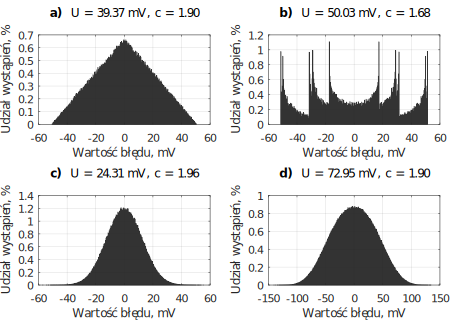
\includegraphics{obrazki/hist_part_S}
\makecaption{fig:symul_partd_hist_S_2_0}{Histogramy realizacji sygnału błędu \textbf{a)}~statycznego, \textbf{b)}~dynamicznego, \textbf{c)}~losowego, \textbf{d)}~wypadkowego wielkości wyjściowej $S_{2,0}$ analizowanego w eksperymencie symulacyjnym toru pomiarowego uzyskane metodą Monte Carlo}
\end{center}
\end{figure}

Na podstawie histogramów przedstawionych na rysunkach~\ref{fig:symul_partd_hist_S_2_0} oraz~\ref{fig:symul_partc_hist_T_1_0} zauważyć można, że oszacowane w równaniach od~\eqref{eq:sym_partd_output_unc_roun_S_2_0} do~\eqref{eq:sym_partd_output_unc_dyn_3_S_2_0} oraz od~\eqref{eq:sym_partd_output_unc_roun_T_1_0} do~\eqref{eq:sym_partd_output_unc_dyn_3_T_1_0} parametry sygnałów błędów pokrywają się z tymi uzyskanymi symulacyjnie. Współczynnik $A_{T_{1,0},s} $ określony w równaniu~\eqref{eq:sym_partd_output_as_T_1_0} wskazujący relacje pomiędzy wejściową i wyjściową wariancją błędów statycznych w przypadku wielkości wyjściowej $T_{1,0}$ jest w przybliżeniu równy zero. W rzeczywistości natomiast, ze względu na niewymierność kolejnych współczynników wiersza macierzy transformacji powiązanych z analizowaną wielkością wyjściową, współczynnik ten jest niezerowy. Fakt ten zauważyć można na podstawie rysunku~\ref{fig:symul_partc_hist_T_1_0}, gdzie teoretycznie wszystkie realizacje błędu statycznego powinny być zerowe. Omawiana rozbieżność jest jednak bardzo niewielka i nie wpływa zupełnie na uzyskane wyniki obliczeń.

\begin{figure}[htb!]
\begin{center}
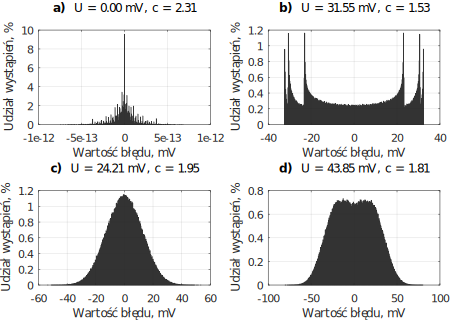
\includegraphics{obrazki/hist_part_T}
\makecaption{fig:symul_partc_hist_T_1_0}{Histogramy realizacji sygnału błędu \textbf{a)}~statycznego, \textbf{b)}~dynamicznego, \textbf{c)}~losowego, \textbf{d)}~wypadkowego wielkości wyjściowej $T_{1,0}$ analizowanego w eksperymencie symulacyjnym toru pomiarowego uzyskane metodą Monte Carlo}
\end{center}
\end{figure}

Ostatecznie wnioskować można, że przeprowadzony eksperyment potwierdził poprawność zaproponowanej metody analizy oraz stworzonego na potrzeby pracy modelu błędów. Oszacowana wartość wariancji dla analizowanych sygnałów błędów była każdorazowo zbieżna z wartością uzyskaną metodą symulacyjną. Uzyskane wartości niepewności rozszerzonych, wyznaczane z użyciem redukcyjnej arytmetyki interwałowej, cechowały się rozbieżnością na poziomie mniejszym, niż wymagany w założeniach pracy. Eksperyment wykazał możliwość stosowania uproszczenia obliczeń, które wynika bezpośrednio z warunków centralnego twierdzenia granicznego. Stosowanie omawianego uproszczenia dopuszczalne jest tylko i wyłącznie w określonych warunkach, natomiast w nieuzasadnionych przypadkach skutkować będzie przekraczającym~\qty{\pm 5}{\percent} błędem oszacowania wartości niepewności rozszerzonej.

Identyczną analizę wykonano wykorzystując budżet niepewności zestawiony w tabeli~\ref{tab:sym_partc_params_unc_list}. Parametry kolejnych składowych sygnałów błędów wyznaczono analogicznie, jak miało to miejsce w przykładach opisanych zależnościami od~\eqref{eq:sym_partd_output_var_stat_S_2_0} do~\eqref{eq:sym_partd_output_var_dyn_3_S_2_0} oraz od~\eqref{eq:sym_partd_output_unc_stat_S_2_0} do~\eqref{eq:sym_partd_output_unc_dyn_3_S_2_0}. W tabelach~\ref{tab:sym_partd_params_unc_list_S_2_0} oraz~\ref{tab:sym_partd_params_unc_list_T_1_0} zestawiono budżety niepewności dla analizowanych wielkości wyjściowych $S_{2,0}$ oraz $T_{1,0}$.

\begin{table}[htb!]
\begin{center}
\makecaption{tab:sym_partd_params_unc_list_S_2_0}{Budżet niepewności wielkości wyjściowej $S_{2,0}$ analizowanego w eksperymencie symulacyjnym toru pomiarowego obejmujący wszystkie źródła błędów}
\begin{tabular}[c]{| c | c | S[table-format = 2.2] | S[table-format = 3.2] | c | c |} \hline
\textbf{Lp.} & \textbf{Symbol} & \textbf{$U$, mV} & \textbf{$\sigma^{2}$, \micro V} & \textbf{Rozkład} & \textbf{Źródło błędu} \\ \hline
1  & ${rw,z}$     & 2.13  &   0.97  & zaokrągleń                   & operacje zmiennoprzecinkowe                \\ \hline
2  & ${rp,q}$     & 13.26 &  45.78  & normalny                     & proces kwantowania ($c$)                   \\ \hline
3  & ${rp,1}$     & 11.80 &  36.26  & normalny                     & nieliniowość obiektu ($a$)                 \\ \hline
4  & ${rp,2}$     & 16.70 &  72.64  & normalny                     & szum wielkości wejściowej                  \\ \hline
5  & ${sp,1}$     & 23.04 &  147.00 & trójkątny                    & dryft temperatury ($a$)                    \\ \hline
6  & ${sp,2}$     & 16.29 &  73.52  & trójkątny                    & dryft temperatury ($b$)                    \\ \hline
7  & ${dp,a,1}$   & 12.32 &  76.40  & \multirow{6}{*}{dwumodalny}  & \multirow{3}{*}{transmitancja ($a$)}       \\ \cline{1-4}
8  & ${dp,a,2}$   & 25.08 &  316.38 &                              &                                            \\ \cline{1-4}
9  & ${dp,a,3}$   & 2.35  &  2.77   &                              &                                            \\ \cline{1-4} \cline{6-6}
10 & ${dp,b,1}$   & 6.07  &  18.52  &                              & \multirow{3}{*}{transmitancja ($b$)}       \\ \cline{1-4}
11 & ${dp,b,2}$   & 12.35 &  76.70  &                              &                                            \\ \cline{1-4}
12 & ${dp,b,3}$   & 1.16  &  0.67   &                              &                                            \\ \hline
\end{tabular}
\end{center}
\end{table}

\begin{table}[htb!]
\begin{center}
\makecaption{tab:sym_partd_params_unc_list_T_1_0}{Budżet niepewności wielkości wyjściowej $T_{1,0}$ analizowanego w eksperymencie symulacyjnym toru pomiarowego obejmujący wszystkie źródła błędów}
\begin{tabular}[c]{| c | c | S[table-format = 2.2] | S[table-format = 3.2] | c | c |} \hline
\textbf{Lp.} & \textbf{Symbol} & \textbf{$U$, mV} & \textbf{$\sigma^{2}$, \micro V} & \textbf{Rozkład} & \textbf{Źródło błędu} \\ \hline
1  & ${rw,z}$     & 1.81  &  0.70   & zaokrągleń                   & operacje zmiennoprzecinkowe                \\ \hline
2  & ${rp,q}$     & 13.26 &  45.78  & normalny                     & proces kwantowania ($c$)                   \\ \hline
3  & ${rp,1}$     & 11.80 &  36.26  & normalny                     & nieliniowość obiektu ($a$)                 \\ \hline
4  & ${rp,2}$     & 16.71 &  72.64  & normalny                     & szum wielkości wejściowej                  \\ \hline
5  & ${sp,1}$     & 0.00  &  0.00   & trójkątny                    & dryft temperatury ($a$)                    \\ \hline
6  & ${sp,2}$     & 0.00  &  0.00   & trójkątny                    & dryft temperatury ($b$)                    \\ \hline
7  & ${dp,a,1}$   & 0.06  &  0.00   & \multirow{6}{*}{dwumodalny}  & \multirow{3}{*}{transmitancja ($a$)}       \\ \cline{1-4}
8  & ${dp,a,2}$   & 3.77  &  7.13   &                              &                                            \\ \cline{1-4}
9  & ${dp,a,3}$   & 19.16 &  184.65 &                              &                                            \\ \cline{1-4} \cline{6-6}
10 & ${dp,b,1}$   & 0.03  &  0.00   &                              & \multirow{3}{*}{transmitancja ($b$)}       \\ \cline{1-4}
11 & ${dp,b,2}$   & 1.85  &  1.73   &                              &                                            \\ \cline{1-4}
12 & ${dp,b,3}$   & 9.44  &  44.82  &                              &                                            \\ \hline
\end{tabular}
\end{center}
\end{table}

Ze względu na korelacje wybranych sygnałów błędów wielkości wejściowych rozważanego algorytmu, wyznaczenie wypadkowych wartości wariancji sygnałów błędów dla kolejnych wielkości wyjściowych przeprowadzane jest zgodnie z zależnością~\eqref{eq:var_matrix}. W dalszej części rozważań przyjęto, że symbol $\mathbfit{\sigma}_{*}$ oznacza wektor złożony z odchyleń standardowych sygnałów błędów składowych wielkości wyjściowej algorytmu, przy czym \enquote{$*$} oznacza symbol analizowanej wielkości wyjściowej. Macierz korelacji oznaczona symbolem $\mathbfit{r}_{d}$ jest jednakowa dla wszystkich wielkości wyjściowych tego algorytmu i składa się z dwunastu wierszy i kolumn, co wynika z liczby analizowanych sygnałów błędów. Przyjmuje się, że kolejne wielkości zawarte w wektorze $\mathbfit{\sigma}_{*}$ oraz kolejne elementy macierzy $\mathbfit{r}_{d}$ są związane z sygnałami błędów zestawionymi w tabelach~\ref{tab:sym_partd_params_unc_list_S_2_0} oraz~\ref{tab:sym_partd_params_unc_list_T_1_0}, a dodatkowo kolejność wyrazów omawianych wielkości jest zgodna z tą daną w tabelach. Wobec powyższych, równanie~\eqref{eq:var_matrix} przyjmuje postać:
\begin{equation}
\sigma_{*,\Sigma}^{2} = \mathbfit{\sigma}_{*}^{T} \cdot \mathbfit{r}_{d} \cdot \mathbfit{\sigma}_{*} \label{eq:sym_partd_output_varmat_list}.
\end{equation}

Uwzględniając pełną dodatnią korelacje pary sygnałów błędów statycznych wzmacniacza i przetwornika pomiarowego przyjmuje się, że $r_{d,sp,1,2} = 1$. Dodatkowo na podstawie danych zawartych w tabelach~\ref{tab:sym_partb_params_dyn_self} oraz~\ref{tab:sym_partb_params_dyn_prop}, współczynniki korelacji kolejnych harmonicznych sygnału błędu dynamicznego o jednakowej częstotliwości są zbliżone do jedności, co wynika z równania~\eqref{eq:dyn_corr}, a zatem $r_{d,dp,a,b,n} = 1$ dla $n \in \{ 1, 2, 3 \}$. Wobec powyższych, kolejne elementy macierzy korelacji $\mathbfit{r}_{d}$ przyjmują wartości:
\begin{equation}
\mathbfit{r}_{d} =
\begin{bmatrix}
\num{1.0} & \num{0.0} & \num{0.0} & \num{0.0} & \num{0.0} & \num{0.0} & \num{0.0} & \num{0.0} & \num{0.0} & \num{0.0} & \num{0.0} & \num{0.0} \\
\num{0.0} & \num{1.0} & \num{0.0} & \num{0.0} & \num{0.0} & \num{0.0} & \num{0.0} & \num{0.0} & \num{0.0} & \num{0.0} & \num{0.0} & \num{0.0} \\
\num{0.0} & \num{0.0} & \num{1.0} & \num{0.0} & \num{0.0} & \num{0.0} & \num{0.0} & \num{0.0} & \num{0.0} & \num{0.0} & \num{0.0} & \num{0.0} \\
\num{0.0} & \num{0.0} & \num{0.0} & \num{1.0} & \num{0.0} & \num{0.0} & \num{0.0} & \num{0.0} & \num{0.0} & \num{0.0} & \num{0.0} & \num{0.0} \\
\num{0.0} & \num{0.0} & \num{0.0} & \num{0.0} & \num{1.0} & \num{1.0} & \num{0.0} & \num{0.0} & \num{0.0} & \num{0.0} & \num{0.0} & \num{0.0} \\
\num{0.0} & \num{0.0} & \num{0.0} & \num{0.0} & \num{1.0} & \num{1.0} & \num{0.0} & \num{0.0} & \num{0.0} & \num{0.0} & \num{0.0} & \num{0.0} \\
\num{0.0} & \num{0.0} & \num{0.0} & \num{0.0} & \num{0.0} & \num{0.0} & \num{1.0} & \num{0.0} & \num{0.0} & \num{1.0} & \num{0.0} & \num{0.0} \\
\num{0.0} & \num{0.0} & \num{0.0} & \num{0.0} & \num{0.0} & \num{0.0} & \num{0.0} & \num{1.0} & \num{0.0} & \num{0.0} & \num{1.0} & \num{0.0} \\
\num{0.0} & \num{0.0} & \num{0.0} & \num{0.0} & \num{0.0} & \num{0.0} & \num{0.0} & \num{0.0} & \num{1.0} & \num{0.0} & \num{0.0} & \num{1.0} \\
\num{0.0} & \num{0.0} & \num{0.0} & \num{0.0} & \num{0.0} & \num{0.0} & \num{1.0} & \num{0.0} & \num{0.0} & \num{1.0} & \num{0.0} & \num{0.0} \\
\num{0.0} & \num{0.0} & \num{0.0} & \num{0.0} & \num{0.0} & \num{0.0} & \num{0.0} & \num{1.0} & \num{0.0} & \num{0.0} & \num{1.0} & \num{0.0} \\
\num{0.0} & \num{0.0} & \num{0.0} & \num{0.0} & \num{0.0} & \num{0.0} & \num{0.0} & \num{0.0} & \num{1.0} & \num{0.0} & \num{0.0} & \num{1.0}
\end{bmatrix}
\label{eq:sym_partd_output_coher_list}.
\end{equation}

Zgodnie z zależnościami~\eqref{eq:sym_partd_output_varmat_list} oraz~\eqref{eq:sym_partd_output_coher_list}, po podstawieniu danych z tabel~\ref{tab:sym_partd_params_unc_list_S_2_0} oraz~\ref{tab:sym_partd_params_unc_list_T_1_0}, otrzymuje się wartości wariancji wypadkowych sygnałów błędów wielkości wyjściowych $S_{2,0}$ oraz $T_{1,0}$, przy czym kolejno:
\begin{gather}
\sigma_{S_{2,0},\Sigma}^{2} = \mathbfit{\sigma}_{S_{2,0}}^{T} \cdot \mathbfit{r}_{d} \cdot \mathbfit{\sigma}_{S_{2,0}} = \qty{1464.79}{\micro V} \label{eq:sym_partd_output_varmat_S_2_0}, \\
\sigma_{T_{1,0},\Sigma}^{2} = \mathbfit{\sigma}_{T_{1,0}}^{T} \cdot \mathbfit{r}_{d} \cdot \mathbfit{\sigma}_{T_{1,0}} = \qty{582.68}{\micro V} \label{eq:sym_partd_output_varmat_T_1_0}.
\end{gather}
Można zauważyć, że wyznaczone w ten sposób wartości są identyczne, jak te wyznaczone wcześniej w równaniach~\eqref{eq:sym_partd_output_var_sum_S_2_0} oraz~\eqref{eq:sym_partd_output_var_sum_T_1_0}.

Występowanie korelacji pomiędzy analizowanymi sygnałami błędów powoduje, że bezpośrednie zastosowanie metody opisanej równaniem~\eqref{eq:unc_matrix} dla współczynników koherencji wyznaczanych zgodnie z równaniem~\eqref{eq:unc_coher} nie jest możliwe. Aby umożliwić zastosowanie omawianej metody, proponuje się wyprowadzenie zależności opisujących wypadkowe parametry niepewności rozszerzonej dla grup skorelowanych sygnałów.

Dla sygnałów błędów statycznych wzmacniacza i przetwornika pomiarowego zapisać można następującą zależność, która określa wypadkową wartość niepewności rozszerzonej analizowanej pary sygnałów:
\begin{equation}
U_{*,sp} = \sqrt{
\begin{bmatrix}
U_{*,sp,1} \\ U_{*,sp,2}
\end{bmatrix}^{T}
\begin{bmatrix}
1 & h_{d,sp,1,2} \\
h_{d,sp,2,1} & 1
\end{bmatrix}
\begin{bmatrix}
U_{*,sp,1} \\ U_{*,sp,2}
\end{bmatrix}}
\label{eq:sym_partd_output_static_corrunc},
\end{equation}
przy czym w przypadku pełnej dodatniej korelacji tych sygnałów, tj. dla $r_{d,sp,1,2} = 1$, zachodzi $h_{d,sp,1,2} = 1$. Podobną zależność opisać można dla kolejnych par skorelowanych sygnałów błędów dynamicznych o jednakowej pulsacji:
\begin{equation}
U_{*,dp,n} = \sqrt{
\begin{bmatrix}
U_{*,dp,a,n} \\ U_{*,dp,b,n}
\end{bmatrix}^{T}
\begin{bmatrix}
1 & h_{d,dp,a,b,n} \\
h_{d,dp,b,a,n} & 1
\end{bmatrix}
\begin{bmatrix}
U_{*,dp,a,n} \\ U_{*,dp,b,n}
\end{bmatrix}}
\label{eq:sym_partd_output_dynamic_corrunc},
\end{equation}
gdzie ze względu na pełną dodatnią korelację zachodzi $h_{d,dp,a,b,n} = 1$. W analizowanych przypadkach, opisanych równaniami~\eqref{eq:sym_partd_output_static_corrunc} oraz~\eqref{eq:sym_partd_output_dynamic_corrunc}, zauważyć można, że wypadkowe sygnały błędów cechować się będą identycznymi kształtami rozkładów, jak ich składowe.

Wobec powyższych, wektor niepewności rozszerzonych kolejnych sygnałów błędów dla wielkości wyjściowych analizowanego toru pomiarowego przedstawić można jako:
\begin{equation}
\mathbfit{U}_{*} =
\begin{bmatrix}
U_{*,rw,z} & U_{*,rp,q} & U_{*,rp,1} & U_{*,rp,2} & U_{*,sp} & U_{*,dp,1} & U_{*,dp,2} & U_{*,dp,3}
\end{bmatrix}
\label{eq:sym_partd_output_unc_sumuvect},
\end{equation}
natomiast macierz koherencji, której wartości wyznaczane są zgodnie z równaniem~\eqref{eq:unc_coher}, opisać można dla kolejnych wielkości wyjściowych w postaci:
\begin{equation}
\mathbfit{h}_{*} =
\begin{bmatrix}
1 & h_{*,0,1} & h_{*,0,2} & h_{*,0,3} & h_{*,0,4} & h_{*,0,5} & h_{*,0,6} & h_{*,0,7} \\
h_{*,1,0} & 1 & h_{*,1,2} & h_{*,1,3} & h_{*,1,4} & h_{*,1,5} & h_{*,1,6} & h_{*,1,7} \\
h_{*,2,0} & h_{*,2,1} & 1 & h_{*,2,3} & h_{*,2,4} & h_{*,2,5} & h_{*,2,6} & h_{*,2,7} \\
h_{*,3,0} & h_{*,3,1} & h_{*,3,2} & 1 & h_{*,3,4} & h_{*,3,5} & h_{*,3,6} & h_{*,3,7} \\
h_{*,4,0} & h_{*,4,1} & h_{*,4,2} & h_{*,4,3} & 1 & h_{*,4,5} & h_{*,4,6} & h_{*,4,7} \\
h_{*,5,0} & h_{*,5,1} & h_{*,5,2} & h_{*,5,3} & h_{*,5,4} & 1 & h_{*,5,6} & h_{*,5,7} \\
h_{*,6,0} & h_{*,6,1} & h_{*,6,2} & h_{*,6,3} & h_{*,6,4} & h_{*,6,5} & 1 & h_{*,6,7} \\
h_{*,7,0} & h_{*,7,1} & h_{*,7,2} & h_{*,7,3} & h_{*,7,4} & h_{*,7,5} & h_{*,7,6} & 1
\end{bmatrix}
\label{eq:sym_partd_output_unc_cohermat},
\end{equation}
przy czym kolejność elementów przedstawionej macierzy odpowiada kolejności elementów w wektorze niepewności rozszerzonych opisanym równaniem~\eqref{eq:sym_partd_output_unc_sumuvect}, gdzie przykładowo $h_{*,0,1} = h_{*,rw,z,rp,q}$. Ostatecznie, wartość wypadkowej niepewności rozszerzonej może być oszacowana zgodnie z równaniem~\eqref{eq:unc_matrix}:
\begin{equation}
U_{*} = \sqrt{\mathbfit{U}_{*} \cdot \mathbfit{h}_{*} \cdot \mathbfit{U}_{*}^{T}} \label{eq:sym_partd_output_unc_totalmat}.
\end{equation}

Podstawiając do równania~\eqref{eq:sym_partd_output_static_corrunc} wartości z tabel~\ref{tab:sym_partd_params_unc_list_S_2_0} oraz~\ref{tab:sym_partd_params_unc_list_T_1_0} otrzymuje się wypadkowe wartości niepewności rozszerzonych dla sygnałów wypadkowych skorelowanych błędów statycznych wielkości $S_{2,0}$ oraz $T_{1,0}$, które wynoszą odpowiednio:
\begin{gather}
\begin{split}
U_{S_{2,0},sp} = & \sqrt{
\begin{bmatrix}
U_{S_{2,0},sp,1} \\ U_{S_{2,0},sp,2}
\end{bmatrix}^{T}
\begin{bmatrix}
1 & h_{d,sp,1,2} \\
h_{d,sp,2,1} & 1
\end{bmatrix}
\begin{bmatrix}
U_{S_{2,0},sp,1} \\ U_{S_{2,0},sp,2}
\end{bmatrix}} = \\ & \sqrt{
\begin{bmatrix}
\num{23.04e-3} \\ \num{16.29e-3}
\end{bmatrix}^{T}
\begin{bmatrix}
1 & 1 \\
1 & 1
\end{bmatrix}
\begin{bmatrix}
\num{23.04e-3} \\ \num{16.29e-3}
\end{bmatrix}} = \qty{39.31}{mV}
\end{split}
\label{eq:sym_partd_output_static_corrunc_S_2_0}, \\
\begin{split}
U_{T_{1,0},sp} = & \sqrt{
\begin{bmatrix}
U_{T_{1,0},sp,1} \\ U_{T_{1,0},sp,2}
\end{bmatrix}^{T}
\begin{bmatrix}
1 & h_{d,sp,1,2} \\
h_{d,sp,2,1} & 1
\end{bmatrix}
\begin{bmatrix}
U_{T_{1,0},sp,1} \\ U_{T_{1,0},sp,2}
\end{bmatrix}} = \\ & \sqrt{
\begin{bmatrix}
\num{0.00} \\ \num{0.00}
\end{bmatrix}^{T}
\begin{bmatrix}
1 & 1 \\
1 & 1
\end{bmatrix}
\begin{bmatrix}
\num{0.00} \\ \num{0.00}
\end{bmatrix}} = \qty{0.00}{mV}
\end{split}
\label{eq:sym_partd_output_static_corrunc__T_1_0},
\end{gather}
natomiast w przypadku równania~\eqref{eq:sym_partd_output_dynamic_corrunc} dla pierwszej harmonicznej sygnałów błędów dynamicznych omawianych wielkości zachodzi:
\begin{gather}
\begin{split}
U_{S_{2,0},dp,1} = & \sqrt{
\begin{bmatrix}
U_{S_{2,0},dp,a,1} \\ U_{S_{2,0},dp,b,1}
\end{bmatrix}^{T}
\begin{bmatrix}
1 & h_{d,dp,a,b,1} \\
h_{d,dp,b,a,1} & 1
\end{bmatrix}
\begin{bmatrix}
U_{S_{2,0},dp,a,1} \\ U_{S_{2,0},dp,b,1}
\end{bmatrix}} = \\ & \sqrt{
\begin{bmatrix}
\num{12.32e-3} \\ \num{6.07e-3}
\end{bmatrix}^{T}
\begin{bmatrix}
1 & 1 \\
1 & 1
\end{bmatrix}
\begin{bmatrix}
\num{12.32e-3} \\ \num{6.07e-3}
\end{bmatrix}} = \qty{18.39}{mV}
\end{split}
\label{eq:sym_partd_output_dynamic_corrunc_S_2_0}, \\
\begin{split}
U_{T_{1,0},dp,1} = & \sqrt{
\begin{bmatrix}
U_{T_{1,0},dp,a,1} \\ U_{T_{1,0},dp,b,1}
\end{bmatrix}^{T}
\begin{bmatrix}
1 & h_{d,dp,a,b,1} \\
h_{d,dp,b,a,1} & 1
\end{bmatrix}
\begin{bmatrix}
U_{T_{1,0},dp,a,1} \\ U_{T_{1,0},dp,b,1}
\end{bmatrix}} = \\ & \sqrt{
\begin{bmatrix}
\num{0.06e-3} \\ \num{0.03e-3}
\end{bmatrix}^{T}
\begin{bmatrix}
1 & 1 \\
1 & 1
\end{bmatrix}
\begin{bmatrix}
\num{0.06e-3} \\ \num{0.03e-3}
\end{bmatrix}} = \qty{0.092}{mV}
\end{split}
\label{eq:sym_partd_output_dynamic_corrunc_T_1_0}.
\end{gather}
Parametry pozostałych harmonicznych sygnałów błędów dynamicznych wyznaczono w analogiczny sposób, zatem obliczenia z nimi związane nie zostały przedstawione. Po podstawieniu uzyskanych wyników do równania~\eqref{eq:sym_partd_output_unc_sumuvect} otrzymuje się wektory składowych niepewności rozszerzonych dla analizowanych wielkości wyjściowych:
\begin{gather}
\mathbfit{U}_{S_{2,0}} =
\begin{bmatrix}
\num{2.13} & \num{13.26} & \num{11.80} & \num{16.71} & \num{39.33} & \num{18.39} & \num{37.42} & \num{3.50}
\end{bmatrix} \cdot \qty{e-3}{V}
\label{eq:sym_partd_output_unc_sumuvect_S_2_0_b}, \\
\mathbfit{U}_{T_{1,0}} =
\begin{bmatrix}
\num{1.81} & \num{13.26} & \num{11.80} & \num{16.71} & \num{0.00} & \num{0.092} & \num{5.62} & \num{28.60}
\end{bmatrix} \cdot \qty{e-3}{V}
\label{eq:sym_partd_output_unc_sumuvect_T_1_0_b},
\end{gather}
przy czym kolejne wyrazy macierzy koherencji dla analizowanych wielkości wyjściowych wyznaczane są zgodnie z równaniem~\eqref{eq:unc_coher}, a zatem przyjmują wartości:
\begin{gather}
\mathbfit{h}_{S_{2,0}} =
\begin{bmatrix}
\num{1.000}  & \num{0.000} & \num{0.000} & \num{0.000} & \num{-0.001} & \num{0.006} & \num{0.017} & \num{0.001} \\
\num{0.000}  & \num{1.000} & \num{0.000} & \num{0.000} & \num{0.006}  & \num{0.033} & \num{0.072} & \num{0.007} \\
\num{0.000}  & \num{0.000} & \num{1.000} & \num{0.000} & \num{0.006}  & \num{0.029} & \num{0.066} & \num{0.006} \\
\num{0.000}  & \num{0.000} & \num{0.000} & \num{1.000} & \num{0.008}  & \num{0.045} & \num{0.086} & \num{0.010} \\
\num{-0.001} & \num{0.006} & \num{0.006} & \num{0.008} & \num{1.000}  & \num{0.116} & \num{0.259} & \num{0.042} \\
\num{0.006}  & \num{0.033} & \num{0.029} & \num{0.045} & \num{0.116}  & \num{1.000} & \num{0.223} & \num{0.028} \\
\num{0.017}  & \num{0.072} & \num{0.066} & \num{0.086} & \num{0.259}  & \num{0.223} & \num{1.000} & \num{0.079} \\
\num{0.001}  & \num{0.007} & \num{0.006} & \num{0.010} & \num{0.042}  & \num{0.028} & \num{0.079} & \num{1.000}
\end{bmatrix}
\label{eq:sym_partd_output_unc_cohermat_S_2_0_b}, \\
\mathbfit{h}_{T_{1,0}} =
\begin{bmatrix}
\num{1.000} & \num{0.000} & \num{0.000} & \num{0.000} & \num{0.000} & \num{0.000} & \num{0.021} & \num{0.021} \\
\num{0.000} & \num{1.000} & \num{0.000} & \num{0.000} & \num{0.000} & \num{0.006} & \num{0.093} & \num{0.092} \\
\num{0.000} & \num{0.000} & \num{1.000} & \num{0.000} & \num{0.000} & \num{0.005} & \num{0.084} & \num{0.084} \\
\num{0.000} & \num{0.000} & \num{0.000} & \num{1.000} & \num{0.000} & \num{0.009} & \num{0.117} & \num{0.116} \\
\num{0.000} & \num{0.000} & \num{0.000} & \num{0.000} & \num{1.000} & \num{0.000} & \num{0.000} & \num{0.000} \\
\num{0.000} & \num{0.006} & \num{0.005} & \num{0.009} & \num{0.000} & \num{1.000} & \num{0.042} & \num{0.042} \\
\num{0.021} & \num{0.093} & \num{0.084} & \num{0.117} & \num{0.000} & \num{0.042} & \num{1.000} & \num{0.497} \\
\num{0.021} & \num{0.092} & \num{0.084} & \num{0.116} & \num{0.000} & \num{0.042} & \num{0.497} & \num{1.000}
\end{bmatrix}
\label{eq:sym_partd_output_unc_cohermat_T_1_0_b}.
\end{gather}
Po podstawieniu powyższych wartości do równania~\eqref{eq:sym_partd_output_unc_totalmat} otrzymuje się wartości wypadkowych niepewności rozszerzonych analizowanych wielkości wyjściowych toru pomiarowego, gdzie kolejno wynoszą one:
\begin{gather}
U_{S_{2,0}} = \sqrt{\mathbfit{U}_{S_{2,0}} \cdot \mathbfit{h}_{S_{2,0}} \cdot \mathbfit{U}_{S_{2,0}}^{T}} = \qty{74.10}{mV} \label{eq:sym_partd_output_unc_totalmat_S_2_0}, \\
U_{T_{1,0}} = \sqrt{\mathbfit{U}_{T_{1,0}} \cdot \mathbfit{h}_{T_{1,0}} \cdot \mathbfit{U}_{T_{1,0}}^{T}} = \qty{43.37}{mV} \label{eq:sym_partd_output_unc_totalmat_T_1_0}.
\end{gather}

Przedstawione w równaniach~\eqref{eq:sym_partd_output_unc_totalmat_S_2_0} oraz~\eqref{eq:sym_partd_output_unc_totalmat_T_1_0} obliczenia wykonano ponownie, dla macierzy koherencji których wartości wyznaczone zostały bez uwzględnienia korekty zaproponowanej w równaniu~\eqref{eq:unc_cohercorra}, tj. kiedy w równaniu~\eqref{eq:unc_coher} przyjmuje się $p_{i,j} = 1$ dla dowolnej pary $i$ oraz $j$. Otrzymane wartości wyniosły kolejno $U_{S_{2,0}} = \qty{77.32}{mV}$ oraz $U_{T_{1,0}} = \qty{46.09}{mV}$. Podobne obliczenia wykonano dla pozostałych wielkości wyjściowych.

W tabeli~\ref{tab:sym_partd_params_unc_sum_b} zestawiono wyniki obliczeń dla pozostałych wielkości wyjściowych oraz te uzyskane w poprzednim eksperymencie, w celu umożliwienia ich porównania. Symbolem $U_{a}$ oznaczono wartości uzyskane przy założeniu normalnego rozkładu sygnału błędu wypadkowego, natomiast symbolem $U_{b}$ oznaczono wartości uzyskane z wykorzystaniem budżetu niepewności opisanego w tabeli~\ref{tab:sym_partc_params_unc_sum}. Wartości oznaczone symbolem $U_{c}$ dotyczą analizy z wykorzystaniem budżetu niepewności opisanego w tabeli~\ref{tab:sym_partc_params_unc_list}, przy czym wielkości oznaczone symbolem $U_{d}$ wyznaczono identycznie, jak $U_{c}$, z tą różnicą, że nie stosowano korekty opisanej równaniem~\eqref{eq:unc_cohercorra} w procesie wyznaczania wartości współczynników koherencji. Podobnie, jak w zestawieniu zawartym w tabeli~\ref{tab:sym_partd_params_unc_sum_a}, wielkości oznaczone symbolem $U_{s}$ dotyczą przeprowadzonego eksperymentu metodą Monte Carlo, natomiast symbolem $\delta_{*}$ oznaczono wyrażony w procentach błąd względny oszacowania wartości niepewności rozszerzonej $U_{*}$ w odniesieniu do wartości $U_{s}$, wyznaczany zgodnie z zależnością~\eqref{eq:unc_error}.

\begin{table}[htb!]
\begin{center}
\makecaption{tab:sym_partd_params_unc_sum_b}{Porównanie uzyskanych przedstawionymi w pracy metodami wartości wypadkowych niepewności rozszerzonych kolejnych wielkości wyjściowych analizowanego w eksperymencie symulacyjnym toru pomiarowego}
\begin{tabular}[c]{| c *{5}{|S[table-format = 2.2]} *{4}{|S[table-format = +1.2]} |} \hline
\multirow{2}{*}{\textbf{Wielkość}} & \multicolumn{5}{c|}{\textbf{Niepewność, mV}} & \multicolumn{4}{c|}{\textbf{Błąd, \%}} \\ \cline{2-10}
& $U_{a}$ & $U_{b}$ & $U_{c}$ & $U_{d}$ & $U_{s}$ & $\delta_{a}$ & $\delta_{b}$ & $\delta_{c}$ & $\delta_{d}$ \\ \hline
$S_{2,0}$ & 75.01 & 74.00 & 74.10 & 77.32 & 72.87 & +2.94 & +1.55 & +1.69 & +6.11 \\ \hline
$S_{2,1}$ & 68.19 & 68.44 & 68.43 & 71.52 & 67.09 & +1.64 & +2.01 & +2.00 & +6.60 \\ \hline
$T_{2,0}$ & 57.29 & 56.26 & 55.91 & 57.58 & 53.89 & +6.31 & +4.40 & +3.75 & +6.85 \\ \hline
$T_{2,1}$ & 58.86 & 55.59 & 55.60 & 59.47 & 54.92 & +7.17 & +1.22 & +1.24 & +8.28 \\ \hline
$T_{1,0}$ & 47.31 & 43.61 & 43.37 & 46.09 & 43.76 & +8.11 & -0.34 & -0.89 & +5.32 \\ \hline
$T_{1,1}$ & 47.31 & 43.60 & 43.37 & 46.08 & 43.74 & +8.16 & -0.32 & -0.85 & +5.35 \\ \hline
$T_{1,2}$ & 47.31 & 43.60 & 43.37 & 46.08 & 43.76 & +8.11 & -0.37 & -0.89 & +5.30 \\ \hline
$T_{1,3}$ & 44.79 & 43.64 & 43.39 & 45.43 & 43.17 & +3.75 & +1.09 & +0.51 & +5.24 \\ \hline
\multicolumn{6}{|c|}{Średnia wartości bezwzględnych wielkości $\delta_{*}$} & 5.77 & 1.41 & 1.48 & 6.13 \\ \hline
\end{tabular}
\end{center}
\end{table}

Analizując wyniki przedstawione w tabeli~\ref{tab:sym_partd_params_unc_sum_b} zauważyć można, że zaproponowana w pracy metoda szacowania wartości wypadkowej niepewności rozszerzonej wraz z zastosowaniem proponowanego modelu błędów zapewniają wyniki zbieżne z tymi uzyskanymi symulacyjnie. Korekta wartości współczynników koherencji opisana równaniem~\eqref{eq:unc_cohercorra} pozwala na znaczne zmniejszenie rozbieżności pomiędzy szacowaną zgodnie z równaniem~\eqref{eq:unc_matrix} wartością, a wartością uzyskiwaną symulacyjnie, w stosunku do wartości uzyskanych bez stosowania opisanej korekty. Wartości uzyskane przy zastosowaniu budżetu niepewności zawierającego jedynie wypadkowe parametry sygnałów błędów z uwzględnieniem na wprowadzone kategorie błędów są zbieżne z wartościami uzyskanymi dla budżetu obejmującego charakterystykę każdego z sygnałów błędów. Rozbieżności pomiędzy wartościami oznaczonymi symbolami $U_{b}$ oraz $U_{c}$ wynikają z innego oszacowania wartości współczynników koherencji.

\section{Podsumowanie rozdziału}

Przedstawione w bieżącym rozdziale rozważania i przeprowadzone eksperymenty potwierdzają poprawność proponowanego w pracy modelu błędów oraz skuteczność stosowanej metody redukcyjnej arytmetyki interwałowej. Oszacowane zgodnie z równaniem~\eqref{eq:unc_matrix} wartości wypadkowej niepewności rozszerzonej dla współczynników koherencji szacowanych zgodnie z zależnością~\eqref{eq:unc_coher} każdorazowo okazywały się zbieżne z wynikami uzyskiwanymi dla przeprowadzonych metodą Monte Carlo eksperymentów. Wartości niepewności rozszerzonych oszacowane stosując zaproponowaną w pracy korektę wartości współczynników koherencji, daną równaniem~\eqref{eq:unc_cohercorra}, były bliższe uzyskanym eksperymentalnie. W praktyce pomiarowej zaproponowana korekta wartości współczynników koherencji nie jest wymagana, jeżeli dopuszcza się przekraczający~\qty{5}{\percent} względny błąd oszacowania wartości wypadkowej niepewności rozszerzonej. Należy również brać pod uwagę, że oszacowane w proponowany sposób wartości niepewności rozszerzonej mogą być w pewnych przypadkach nieco niższe, niż wartości prawdziwe. Różnice te nie przekraczają zwykle około~\qty{-2.5}{\percent} wartości prawdziwej, co wykazano w eksperymencie, którego wyniki przedstawiono wcześniej na rysunku~\ref{fig:hist_reductive}.

W przypadku, gdy analizowane sygnały błędów składowych cechować się będą nietypowym rozkładem realizacji tych sygnałów, stosowanie omawianej w pracy metody wymagać będzie wyznaczenia wartości współczynników kształtu dla wszystkich analizowanych typów rozkładów. Jest to jedyna czynność, której przeprowadzenie nie będzie mogło zwykle odbywać się w czasie pracy systemu pomiarowego i będzie musiała ona zostać przeprowadzona na etapie identyfikacji jego właściwości~\cite{auth_reductive}. Podobny problem napotkać można w przypadku wystąpienia korelacji pomiędzy analizowanymi sygnałami błędów składowych -- należy wtedy postąpić identycznie, jak pokazano w przykładzie lub zastosować inną metodę wyznaczania wartości elementów macierzy koherencji, jak chociażby pokazano w pracy~\cite{jakubiec_reductive}.

Przedstawiona w równaniach od~\eqref{eq:sym_partd_output_static_corrunc} do~\eqref{eq:sym_partd_output_unc_totalmat} analiza umożliwiła wykorzystanie zaproponowanej metody szacowania wartości współczynników koherencji, opisanej równaniem~\eqref{eq:unc_coher} Mimo że metoda ta nie jest odpowiednia dla analizy skorelowanych sygnałów. Możliwość zastosowania opisanego algorytmu wynika z faktu, że wypadkowe sygnały dla skorelowanych grup sygnałów cechują się typowym kształtem rozkładu, dla którego wyznaczono wcześniej wartości współczynników kształtu. W innych okolicznościach należałoby wyznaczyć odpowiednie dla analizowanych parametrów sygnałów wartości współczynników koherencji.

Jako że żaden z etapów szacowania wartości wypadkowej niepewności rozszerzonej zgodnie z zaproponowaną metodą nie wymaga przeprowadzania dodatkowych symulacji metodą Monte Carlo, a wykonywane obliczenia sprowadzają się w większości przypadków do prostych operacji arytmetycznych, przedstawiona metoda może zostać zaimplementowana w torze pomiarowym w celu bieżącej oceny jego właściwości metrologicznych. W przypadku zmiany parametrów sygnałów błędów obecnych w analizowanym torze pomiarowym wymagane jest jedynie ponowne wyznaczenie wartości macierzy koherencji i wskazanie parametrów istniejących sygnałów błędów. Istotnymi parametrami analizowanych sygnałów błędów jest w tym przypadku wartość niepewności rozszerzonej dla wybranego, identycznego dla wszystkich wielkości poziomu ufności oraz rodzaj rozkładu realizacji analizowanego sygnału.

Stosowanie uproszczenia, gdzie zakłada się normalny rozkład realizacji sygnału błędu wypadkowego, pozwala znacznie uprościć proces wyznaczania wartości wypadkowej niepewności rozszerzonej i zastąpić konieczność stosowania zależności~\eqref{eq:unc_matrix} oraz~\eqref{eq:unc_coher} wyznaczeniem wariancji wypadkowego sygnału błędu. Stosowanie omawianego uproszczenia wymaga posiadania pewności odnoście spełnienia warunków centralnego twierdzenia granicznego. Jak wykazały przeprowadzone eksperymenty, nawet dla kilkunastu źródeł błędów, gdzie większość z nich nie jest wzajemnie skorelowana, założenie to może okazać się niespełnione, co skutkuje znaczną rozbieżnością pomiędzy oszacowaną, a prawdziwą wartością niepewności rozszerzonej na poziomie zbliżonym do~\qty{\pm 10}{\percent}.

Mimo że wprowadzenie do proponowanego modelu błędów funkcji przetwarzania obiektu może być zastąpione wprowadzeniem statycznego wzmocnienia w równaniu transmitancji obiektu, obecność tej funkcji umożliwia bardziej spójną i logiczną analizę rzeczywistych obiektów. Nawet, jeśli rzeczywista postać funkcji przetwarzania nie jest znana, to wprowadzany przez nią sygnał błędu można opisać odpowiednią zależnością lub wskazać jego parametry, jak pokazano w omówionym przykładzie. Przeprowadzone badania wykazały, że w przypadku nieznanej rzeczywistej funkcji przetwarzania obiektu do oszacowania wpływu tej funkcji na postać sygnałów na wyjściu obiektu, wykorzystać można jej idealne równanie przetwarzania. Wskazana właściwość jest bardzo cenna w przypadku nieliniowości charakterystyki obiektu lub analizy przetwornika analogowo-cyfrowego.

\chapter{Pomiarowa weryfikacja tezy}

Ostatni etap weryfikacji postawionej w pracy tezy stanowi analiza właściwości metrologicznych przykładowego toru pomiarowego, który stworzony został na potrzeby pracy. Analizowany tor pomiarowy przetwarza zmienny w czasie sygnał napięciowy $s(t)$ o chwilowej wartości napięcia z przedziału $<0;1>~\unit{V}$. W celu dopasowania poziomu sygnału napięcia wejściowego do zakresu napięcia wejściowego przetwornika analogowo-cyfrowego oraz zwiększenia impedancji wejściowej toru pomiarowego, sygnał $s(t)$ podawany jest na wejście wzmacniacza pomiarowego. Sygnał wyjściowy wzmacniacza $y(t)$ przetwarzany jest na postać cyfrową $c(i)$, a następnie po wykonaniu odtwarzania statycznego, podawany jest w postaci wielkości $x(i)$ na wejście jednostki \enquote{DSP}, która pobiera $N$ próbek tego sygnału i wyznacza na ich podstawie $M$ wartości wielkości wyjściowych toru pomiarowego, stosując w tym celu algorytm dyskretnej transformacji falkowej. Schemat blokowy omawianego toru pomiarowego przedstawiono na rysunku~\ref{fig:chain_real}.

\begin{figure}[htb!]
\begin{center}
\includegraphics{obrazki/schemat_real}
\makecaption{fig:chain_real}{Schemat blokowy stworzonego na potrzeby pracy toru pomiarowego będącego obiektem przeprowadzanego eksperymentu}
\end{center}
\end{figure}

Do realizacji układu wzmacniacza pomiarowego zastosowany został wzmacniacz operacyjny \enquote{MCP6002}~\cite{microchip_manual} w konfiguracji nieodwracającej, o docelowym wzmocnieniu wynoszącym~\qty{3.3}{V \per V}. Napięcie zasilania wzmacniacza wynosi~\qty{3.3}{V} i pochodzi ze stabilizatora \enquote{LD1117}~\cite{stm_manual} typu \enquote{LDO} (ang. \enquote{Low Dropout}). Zaproponowana konfiguracja, zgodnie z wcześniejszymi założeniami, zapewnia wysoką impedancję wejściową toru pomiarowego oraz bardzo niską impedancję wyjściową wzmacniacza. Parametry statyczne oraz dynamiczne analizowanego obiektu wymagają identyfikacji, ze względu na niedostateczne informacje zawarte w dokumentacji wykorzystanego układu oraz nieznajomości dokładnego modelu dla zastosowanej aplikacji. Należy zauważyć, że dokładna analiza zastosowanego układu byłaby skomplikowana i nie jest konieczna do oceny jego właściwości metrologicznych związanych z zastosowanie proponowanego w pracy modelu błędu.

Zastosowany przetwornik analogowo-cyfrowy stanowi $12$-bitowy przetwornik wagowy~\enquote{SAR} (ang. \enquote{Successive Approximation Register}), wbudowany w mikrokontroler \enquote{STM32F411}~\cite{stm_f411}. Źródło napięcia odniesienia stanowi w jego przypadku stabilizator \enquote{AP7343}~\cite{diodes_manual} typu \enquote{LDO}, o znamionowym napięciu wyjściowym równym~\qty{3.3}{V}, przyłączony z użyciem dodatkowego filtru LC. Przetwornik analogowo-cyfrowy taktowany jest wewnętrznym sygnałem zegarowym o częstotliwości~\qty{24}{MHz}, przy czym próbkowanie wyzwalane jest sygnałem z licznika, którego częstotliwość wyzwalania wynosi~\qty{48}{kHz}. Częstotliwość próbkowania analizowanego toru pomiarowego wynosi zatem $f_{s} = \qty{48}{kHz}$. Na proces konwersji analogowo-cyfrowej przypada proces kluczowania napięcia wejściowego trwający $15$ taktów zegara, po którym następuje konwersja trwająca $15$ taktów zegara, co w analizowanym przypadku stanowi czas~\qty{625}{ns} dla każdej z operacji. Łączny czas konwersji analogowo-cyfrowej pojedynczej próbki sygnału wejściowego $y(t)$ na jego dyskretną reprezentację $c(i)$ wynosi zatem~\qty{1250}{ns}. Ze względu na typową aplikacje omawianego przetwornika, jego parametry metrologiczne mogą zostać pozyskane z dokumentacji producenta układu~\cite{stm_f411}.

Pozyskane próbki napięcia $x(i)$, stanowiące dyskretną reprezentację sygnału wejściowego $s(t)$, zapisywane są w wektorze $\mathbf{x}$ o długości $N = 128$. Wektor wielkości wejściowych $\mathbf{x}$ podawany jest na wejście algorytmu dyskretnej transformacji falkowej, którego implementacja zrealizowana została z wykorzystaniem instrukcji \enquote{DSP} dostępnych dla zastosowanego mikrokontrolera~\cite{reay_dsp}. Analizowany algorytm wykorzystuje falkę \enquote{spline4:4}~\cite{wang_splinebasics} dla pięciu iteracji procesu dekompozycji sygnału. Zgodnie z równaniem~\eqref{eq:alg_out_mat} wyznaczanych jest $M = 128$ próbek wektora wielkości wyjściowych $\mathbf{X}$, które stanowią wyjście dla pojedynczej serii pomiarowej analizowanego toru pomiarowego. Wartości elementów macierzy transformacji $\mathbf{A}$ zidentyfikowano zgodnie z metodoą przedstawioną w równaniu~\eqref{eq:wt_ident}, wykorzystując w tym celu implementacje algorytmu transformacji falkowej dostępną w programie \enquote{GNU Octave}~\cite{pruuvsa_dwt}. Czas obliczeń wynosi w analizowanym przypadku~\qty{1508}{\micro s}, przy czym łączny czas akwizycji pojedynczego wektora próbek wielkości wejściowych wynosi~\qty{2666.6(6)}{\micro s}. Podczas obliczeń stosowane są liczby zmiennoprzecinkowe o długości słowa $32$-bitów.

Przedstawiony tor pomiarowy pracuje w trybie ciągłym, tj. w pojedynczym oknie pomiarowym, podczas pobierania próbek wielkości wejściowych wektora $\mathbf{x}$, wyznaczana jest realizacja wektora wielkości wyjściowych $\mathbf{X}$ dla poprzedniej realizacji wektora wielkości wejściowych. Wykorzystywany jest w tym celu kontroler \enquote{DMA} (ang. \enquote{Direct Memory Access}), nadzorujący proces buforowania kolejnych realizacji sygnału $x(i)$, w czasie gdy program główny wykonuje obliczenia dane równaniem~\eqref{eq:alg_out_mat}. Analiza wartości wielkości wyjściowych omawianego toru pomiarowego jest możliwa między innymi po podłączeniu go do komputera klasy \enquote{PC} za pośrednictwem portu \enquote{USB}, przy czym wykorzystywany jest w tym celu układ peryferyjny \enquote{USB OTG Full-Speed}, zintegrowany w zastosowanym mikrokontrolerze.

W dalszej części rozdziału opisano najważniejsze źródła błędów analizowanego toru pomiarowego, a następnie wykorzystano zaproponowany w pracy model błędu do opisu właściwości wykazanych sygnałów błędów. Ze względu na fakt, że nie jest znany dokładny model analizowanego toru pomiarowego, przeprowadzono identyfikację jego właściwości, istotnych ze względu na zaproponowany model błędu. W ostatniej części rozdziału opisano przeprowadzony eksperyment pomiarowy, wykorzystujący metodę Monte-Carlo, mający na celu ocenę poprawności przedstawionych rozważań i weryfikacje możliwości praktycznej aplikacji zawartych w pracy propozycji. Temperatura otoczenia podczas przeprowadzania eksperymentów była stała i wynosiła~\qty{21}{\degreeCelsius}.

\section{Identyfikacja właściwości toru pomiarowego}

Pierwszą grupą identyfikowanych właściwości analizowanego toru pomiarowego będą jego właściwości statyczne. Właściwości te nie zależą od częstotliwości przetwarzanego sygnału i wynikać będą z charakterystyk przetwarzania statycznego kolejnych fragmentów tego toru. Jako, że z punktu widzenia przeprowadzanej analizy właściwości metrologicznych oraz właściwości zaproponowanej w pracy metody analizy, najistotniejsze informacje stanowić będą dane dotyczące parametrów sygnałów błędów na wejściu algorytmu dyskretnej transformacji falkowej, najbardziej przystępne z punktu widzenia projektanta toru pomiarowego będzie wyznaczenie tych parametrów traktując całość toru pomiarowego znajdującego się przed tym algorytmem, jak jeden obiekt.

Wobec powyższych, proponuje się wyznaczenie charakterystyki statycznej $f_{c}(x)$ dla wielkości wyjściowej $c(i)$ przetwornika analogowo-cyfrowego, a następnie na jej podstawie określenie funkcji odtwarzania $f_{x}(x)$. Należy w tym celu na wejście toru pomiarowego podawać, z wzorcowego źródła napięcia, napięcie stałe o zadanej wartości, a następnie pobierać wielokrotnie wartość realizacji wielkości wyjściowej $\hat{c}(i)$ przetwornika analogowo-cyfrowego, którą następnie należy uśrednić dla przeprowadzonej serii pomiarów. Podczas eksperymentu na wejście toru pomiarowego podawano napięcie stałe z zakresu $<0;1>~\unit{V}$ z krokiem wynoszącym~\qty{12.5}{mV}, a na pojedynczą serię pomiarową składało się trzydzieści tysięcy próbek wielkości wyjściowej przetwornika analogowo-cyfrowego. Źródło napięcia wejściowego stanowił w przeprowadzonym eksperymencie kalibrator FLUKE 5700A~\cite{fluke_manual}, stąd założyć można, że przetwarzany sygnał $s(t)$ nie zawierał żadnych sygnałów błędów, a zatem wszystkie sygnały błędów obecne w torze pomiarowym stanowiły błędy własne tego toru.

Na podstawie przeprowadzonych pomiarów, po wykonaniu aproksymacji liniowej metodą najmniejszych kwadratów, przebieg sygnału $c(i)$ opisać można równaniem:
\begin{equation}
c \emb{i} = f_{c} \emb{f_{y} \emb{s \emb{iT_{p}}}} = 4.0956 \cdot s \emb{iT_{p}} + 4.1764 \label{eq:pom_func_static}.
\end{equation}
Zakładając, że czułość wielkości $x(i)$ w stosunku do wielkości $s(t)$ wynosi~\qty{1}{V \per V}, przebieg sygnału $x(i)$ w funkcji wielkości $c(i)$ można opisać jako:
\begin{equation}
x \emb{i} = f_{x} \emb{c \emb{i}} = f_{x} \emb{f_{c} \emb{f_{y} \emb{s \emb{iT_{p}}}}} = \frac{c \emb{i} - 4.1764}{4.0956} = s \emb{iT_{p}} \label{eq:pom_funx_static}.
\end{equation}
Odchylenie standardowe średnich wartości $\overline{c}(i)$ uzyskanych dla kolejnych serii pomiarowych od charakterystyki danej równaniem~\eqref{eq:pom_func_static} wyniosło $\sigma_{c,nl} = \qty{0.56}{kwantu}$, co interpretować można jako niepewność standardową nieliniowości charakterystyki statycznej przetwarzania wielkości $c(i)$. Po wykonaniu odtwarzania statycznego, zgodnie z równaniem~\eqref{eq:pom_funx_static}, niepewność standardowa związana z nieliniowością charakterystyki odtwarzania wielkości $x(i)$ wynosi odpowiednio $\sigma_{x,nl} = \qty{0.14}{mV}$.

Poza nieliniowością charakterystyki odtwarzania sygnału $x(i)$ w budżecie niepewności uwzględnić należy występowanie pozostałych czynników zakłócających proces pomiaru. Czynniki te stanowią między innymi zakłócenia wynikające z fluktuacji napięcia zasilania wzmacniacza pomiarowego oraz napięcia odniesienia przetwornika analogowo-cyfrowego, błędy kwantowania, niejednorodność wzorców struktury wewnętrznej przetwornika analogowo-cyfrowego, czy szumy występujące w części analogowej toru pomiarowego. Jako, że z punktu widzenia proponowanego w pracy modelu błędu, istotne są jedynie parametry wypadkowego sygnału błędu $e_{x,rw}(i)$ opisanego równaniem:
\begin{equation}
e_{x,rw} \emb{i} = \tilde{x} \emb{i} - \dot{s} \emb{iT_{p}} \label{eq:pom_funx_error},
\end{equation}
parametry te można zidentyfikować na podstawie przeprowadzonego eksperymentu pomiarowego. Definiując sygnał błędu $e_{c,rw}(i)$ w postaci:
\begin{equation}
e_{c,rw} \emb{i} = \tilde{c} \emb{i} - f_{c} \emb{f_{y} \emb{\dot{s} \emb{iT_{p}}}} \label{eq:pom_func_error},
\end{equation}
istnieje możliwość sporządzenia na podstawie wykonanych pomiarów histogramu, a następnie zgodnie z równaniem~\eqref{eq:unc_summation} wyznaczenia niepewności rozszerzonej związanej z sygnałem błędu $e_{c,rw}(i)$. Oszacowana wartość niepewności $U_{c,rw}$ związana z właściwościami statycznymi analizowanego fragmentu toru pomiarowego wyniosła $U_{c,rw} = \qty{2.54}{kwantu}$. Biorąc pod uwagę zależność daną równaniem~\eqref{eq:pom_funx_static} niepewność związana z sygnałem błędu $e_{x,rw}(i)$ w analizowanym przypadku właściwości statycznych wynosi odpowiednio $U_{x,rw} = \qty{0.62}{mV}$. Wyniki pomiarów wielkości $\overline{c}(i)$ w funkcji napięcia wejściowego dla przeprowadzonych serii pomiarowych oraz histogram uzyskanych realizacji sygnału błędu $e_{c,rw}(i)$ przedstawiono na rysunku~\ref{fig:pom_static_fun}.

\begin{figure}[htb!]
\begin{center}
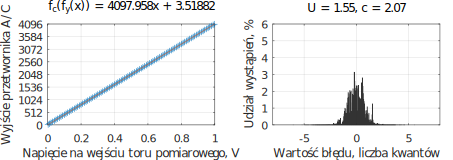
\includegraphics{obrazki/static_adcout}
\makecaption{fig:pom_static_fun}{Zależność wartości wielkości wyjściowej przetwornika analogowo-cyfrowego w funkcji wartości napięcia wejściowego analizowanego toru pomiarowego oraz histogram uzyskanych realizacji błędu statycznego wielkości wyjściowej przetwornika analogowo-cyfrowego}
\end{center}
\end{figure}

Należy zaznaczyć, że z punktu widzenia proponowanego modelu błędu dokładna znajomość postaci funkcji przetwarzania statycznego każdego elementu toru pomiarowego nie jest znana. Przykładowo, pomimo udziału funkcji przetwarzania $f_{y}(x)$ wzmacniacza pomiarowego w równaniach~\eqref{eq:pom_func_static} oraz~\eqref{eq:pom_funx_static}, znajomość tej funkcji nie jest konieczna podczas omawianej analizy. Dodatkowo, na podstawie treści przedstawionych równań zauważyć można, że na etapie przetwarzania wielkości $c(i)$ wprowadzane jest przesunięcie charakterystyki statycznej, które najprawdopodobniej spowodowane jest błędem zera wzmacniacza pomiarowego. Opisywana sytuacja powoduje, że funkcja przetwarzania nie spełnia właściwości addytywności, przez co nie jest możliwa analiza każdego sygnału błędu z osobna, jak proponowano w opisanym w pracy modelu błędu. Przeprowadzenie analizy z punktu widzenia wielkości wejściowej algorytmu dyskretnej transformacji falkowej umożliwia eliminację opisywanych niedogodności i wykorzystanie równań od~\eqref{eq:out_disc_err_stat_self} do~\eqref{eq:out_disc_err_rand_prop}, umożliwiających analizę z zastosowaniem metody superpozycji dla obecnych w torze pomiarowym sygnałów błędów.

Analizując dokumentacje~\cite{microchip_manual, stm_manual, diodes_manual, stm_f411} kolejnych komponentów toru pomiarowego zauważyć można, że najistotniejsze źródło błędów związanych z właściwościami statycznymi stanowi w analizowanym przypadku przetwornik analogowo-cyfrowy. Zgodnie z dokumentacją~\cite{stm_f411}, typowa wartość błędu granicznego wielkości wyjściowej $c(i)$ dla zbliżonych do stosowanych w sporządzonej aplikacji parametrów pracy przetwornika analogowo-cyfrowego powinna mieścić się w przedziale $\pm<2; 3>~\unit{LSB}$, co pokrywa się z wartością uzyskaną na podstawie histogramu przedstawionego na rysunku~\ref{fig:pom_static_fun}. Najważniejsze źródła błędu, które zdefiniowane są przez producenta zastosowanego przetwornika analogowo-cyfrowego obejmują: błąd przesunięcia charakterystyki względem zera, błąd wzmocnienia, całkowy błąd nieliniowości i różnicowy błąd nieliniowości~\cite{stm_adc}. Przeprowadzony eksperyment pozwolił zidentyfikować wypadkowe parametry sumy opisanych sygnałów błędów, przy czym należy zauważyć, że ze względu niewielką w stosunku do rozdzielczości przetwornika liczbę serii pomiarowych, nie udało się uzyskać większości realizacji różnicowego błędu nieliniowości. Na podstawie wyników eksperymentu oraz informacji zawartych w dokumentach~\cite{stm_f411, stm_adc} można jednak przyjąć, że wartość niepewności $U_{c,rw}$ została oszacowana prawidłowo. Ze względu na niewielką liczbę realizacji różnicowego błędu nieliniowości można zakładać, że rzeczywisty rozkład błędu $e_{c,rw}(i)$ będzie rozkładem normalnym, co wynika z warunków centralnego twierdzenia granicznego~\cite{jcgm_guide}.

Drugą grupę właściwości stanowią właściwości dynamiczne. Podobnie, jak w przypadku właściwości statycznych, istnieje możliwość ich identyfikacji pomiarowej, uzyskując kolejne realizacje wielkości wyjściowej $c(i)$. Przypadek właściwości dynamicznych jest jednak złożony i wymaga stosowania bardziej skomplikowanej procedury pomiarów -- konieczna bowiem jest odpowiednia synchronizacja przebiegu napięcia wejściowego toru pomiarowego z przebiegiem sygnału wyjściowego przetwornika analogowo-cyfrowego, w celu oszacowania różnicy pomiędzy fazami analizowanych sygnałów. Opisywana procedura jest zatem kłopotliwa, a dodatkowo podczas jej realizacji wprowadzany byłby kolejny błąd, związany z opisywaną synchronizacją. Wobec powyższych okoliczności proponuje się w pierwszej kolejności identyfikację właściwości dynamicznych zastosowanego wzmacniacza pomiarowego, a następnie ustalenie właściwości dynamicznych przetwornika analogowo-cyfrowego na podstawie jego dokumentacji~\cite{stm_f411}, która szczegółowo opisuje model tego przetwornika.

W przypadku wzmacniacza pomiarowego proponowana procedura identyfikacji jego właściwości polega na podawaniu na wejście analizowanego wzmacniacza napięcia sinusoidalnie zmiennego o zadanej pulsacji i stałej amplitudzie. Dla zadanych parametrów sygnału wejściowego $s(t)$ zmierzyć należy amplitudę sygnału wyjściowego $y(t)$ wzmacniacza, potrzebną do wyznaczenia jego wzmocnienia $K_{y}(\omega)$, oraz przesunięcie fazowe $\varphi_{y}(\omega)$ pomiędzy sygnałem wejściowym i wyjściowym. Pomiędzy omawianymi wielkościami zachodzą następujące relacje:
\begin{gather}
K_{y} \emb{\omega} = \frac{A_{wy} \emb{\omega}}{A_{we} \emb{\omega}} \label{eq:pom_dyn_amp}, \\
\varphi_{y} \emb{\omega} = \varphi_{wy} \emb{\omega} - \varphi_{we} \emb{\omega} = -\omega \cdot \Delta t \emb{\omega} \label{eq:pom_dyn_phi},
\end{gather}
gdzie w funkcji pulsacji $A_{wy}$ jest amplitudą sygnału wyjściowego, $A_{we}$ amplitudą sygnału wejściowego, $\varphi_{wy}$ przesunięciem fazowym sygnału wyjściowego, $\varphi_{we}$ przesunięciem fazowym sygnału wejściowego wzmacniacza, natomiast $\Delta t$ opóźnieniem sygnału wyjściowego względem sygnału wejściowego.

Omawiany eksperyment przeprowadzono wykorzystując jako źródło napięcia wejściowego analizowanego wzmacniacza generator przebiegów arbitralnych RIGOL DG1011~\cite{rigol_fawg}. W celu oszacowania parametrów opisanych równaniami~\eqref{eq:pom_dyn_amp} oraz~\eqref{eq:pom_dyn_phi} zastosowano oscyloskop RIGOL DS5062MA~\cite{rigol_dso}. Na podstawie pozyskanych danych oszacowano pasmo przenoszenia analizowanego wzmacniacza, któremu dla zastosowanej konfiguracji układu odpowiadała częstotliwość graniczna $f_{y,g} \approx \qty{172}{kHz}$ oraz wzmocnienie statyczne $k_{y,a} = \qty{3.27}{V \per V}$. Dla przedstawionych charakterystyk sporządzono dwa modele aproksymacji. W modelu pierwszym wykorzystano funkcję opisującą transmitancję wzmacniacza w postaci:
\begin{gather}
\tilde{G}_{y,a} \emb{j\omega} = \frac{k_{y,a}}{1 + j \frac{\omega}{2 \pi f_{y,g}}} = \frac{k_{y,a}}{\frac{\omega^{2}}{4 \pi^{2} f_{y,g}^{2}} + 1} - j \frac{\omega k_{y,a}}{2 \pi f_{y,g} \left( \frac{\omega^{2}}{4 \pi^{2} f_{y,g}^{2}} + 1 \right) } \label{eq:pom_dyn_trans},
\end{gather}
natomiast dla modelu drugiego wykonano metodą najmniejszych kwadratów aproksymacje wielkości opisanych równaniami~\eqref{eq:pom_dyn_amp} oraz~\eqref{eq:pom_dyn_phi} przy użyciu funkcji:
\begin{gather}
\tilde{K}_{y,b} \emb{\omega} = 3.395 - 0.125 \exp \emb{\num{1.789e-6} \omega} \label{eq:pom_aprox_amp}, \\
\tilde{\varphi}_{y,b} \emb{\omega} = -\frac{1.700 \omega^{5}}{\num{e30}} + \frac{6.517 \omega^{4}}{\num{e24}} - \frac{7.932 \omega^{3}}{\num{e18}} + \frac{2.921 \omega^{2}}{\num{e12}} - \frac{6.924 \omega}{\num{e07}} \label{eq:pom_aprox_phi}.
\end{gather}
Uzyskane dla sygnału o częstotliwościach z zakresu $<0.1; 250>~\unit{kHz}$ wartości wzmocnienia i przesunięcia fazowego oraz odpowiadające im aproksymacje dla modeli opisanych w równaniach od~\eqref{eq:pom_dyn_trans} do~\eqref{eq:pom_aprox_phi} przedstawiono na rysunku~\ref{fig:pom_dynamic_ampout}.

\begin{figure}[htb!]
\begin{center}
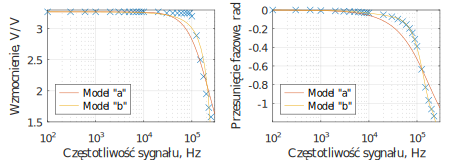
\includegraphics{obrazki/dynamic_ampout}
\makecaption{fig:pom_dynamic_ampout}{Zależność wartości wzmocnienia oraz przesunięcia fazowego w funkcji częstotliwości dla zastosowanej konfiguracji wzmacniacza pomiarowego}
\end{center}
\end{figure}

Analizując przedstawione wykresy zauważyć można, że model zaproponowany w równaniach~\eqref{eq:pom_aprox_amp} oraz~\eqref{eq:pom_aprox_phi} stanowi akceptowalne przybliżenie charakterystyki analizowanego wzmacniacza pomiarowego, natomiast model dany równaniem~\eqref{eq:pom_dyn_trans} odbiega od niej znacząco, przez co nie może być stosowany. Wobec powyższych przyjmuje się, że równania~\eqref{eq:pom_aprox_amp} oraz~\eqref{eq:pom_aprox_phi} opisywać będą właściwości dynamiczne zastosowanego wzmacniacza, odpowiadające zależnościom~\eqref{eq:mid_cont_amp} oraz~\eqref{eq:mid_cont_phi}, a zatem zachodzi $\tilde{K}_{y}(\omega) = \tilde{K}_{y,b}(\omega)$ oraz $\tilde{\varphi}_{y}(\omega) = \tilde{\varphi}_{y,b}(\omega)$. Należy zauważyć, że na potrzeby zaproponowanego w pracy modelu błędu pozyskane w wyniku przeprowadzonego eksperymentu informacje będą wystarczające i nie jest konieczna znajomość dokładnej postaci funkcji opisującej transmitancję analizowanego obiektu.

Ostatni etap identyfikacji właściwości dynamicznych obejmuje właściwości przetwornika analogowo-cyfrowego. Zgodnie z dokumentacją~\cite{stm_f411} obwód zastępczy części analogowej przetwornika analogowo-cyfrowego przedstawić można w postaci modelu filtra dolno-przepustowego typu \enquote{RC}, przy czym stanowić on będzie kaskadowe połączenie dwóch takich filtrów, co przedstawiono na rysunku~\ref{fig:pom_schemat_adc}. Wypadkowa pojemność $C_{we}$ wynika w analizowanym przypadku z pojemności w obrębie wyprowadzenia mikrokontrolera, natomiast pojemność $C_{adc}$ wynika pojemności wewnętrznej układu próbkująco-pamiętającego. Zgodnie z dokumentacją wewnętrzna pojemność przetwornika wynosi typowo około~\qty{4}{pF}, natomiast pojemność zastępcza $C_{we}$ obwodu wejściowego przetwornika wynosi zwykle około~\qty{5}{pF}. Rezystancję $R_{we}$ w zaproponowanym modelu stanowi szeregowe połączenie rezystancji doprowadzeń pomiędzy wzmacniaczem pomiarowym i mikrokontrolerem oraz rezystancji wyjściowej wzmacniacza, przy czym w omawianym przypadku jest to wartość rzędu pojedynczych Ohmów. Rezystancja $R_{adc}$ jest rezystancją klucza układu próbkująco-pamiętającego i, zgodnie z dokumentacją, jej wartość nie przekracza~\qty{6}{k\ohm}. Dodatkowe elementy, które można zauważyć na omawianym schemacie, to diody zabezpieczające wejście mikrokontrolera przed zbyt wysokim lub zbyt niskim napięciem wejściowym oraz źródło $I_{adc}$, które zastępuje upływność układu nieprzekraczającą~\qty{\pm 1}{\micro A}. Elementy te mogą być pominięte w omawianej analizie, ze względu na ich znikome znaczenie w budżecie błędów analizowanego toru pomiarowego.

\begin{figure}[htb!]
\begin{center}
\includegraphics{obrazki/schemat_adc}
\makecaption{fig:pom_schemat_adc}{Schemat zastępczy modelu przetwornika analogowo-cyfrowego zastosowanego w analizowanym torze pomiarowym zgodny z dokumentacją producenta układu~\cite{stm_f411}}
\end{center}
\end{figure}

Pierwszy filtr, który przedstawiono na rysunku~\ref{fig:pom_schemat_adc}, składa się z rezystancji rzędu pojedynczych Ohmów oraz pojemności rzędu mikro Faradów. Pozwala to oszacować częstotliwość graniczną tego filtru na poziomie kilkuset giga Herców. Filtr drugi stanowi połączenie rezystancji rzędu kilo Ohmów z pojemnością rzędu piko Faradów, a zatem rząd wielkości częstotliwości granicznej takiego filtru oszacować można na poziomie kilkuset mega Herców. Na podstawie przedstawionych parametrów modelu analizowanego przetwornika analogowo-cyfrowego, przyjąć można pomijalnie mały udział jego właściwości dynamicznych w puli właściwości dynamicznych całego toru pomiarowego. Ostateczna analiza właściwości dynamicznych całości toru pomiarowego uwzględniać może jedynie właściwości dynamiczne zastosowanego wzmacniacza pomiarowego, którego pasmo przenoszenia jest znacznie niższe.

Ostatnim fragmentem toru pomiarowego, który wprowadzać może do sygnału wyjściowego dodatkowe błędy, jest algorytm dyskretnej transformacji falkowej. Przeprowadzone wcześniej badania, których wyniki przedstawiono w tabeli~\ref{tab:varnum_spline4_4_5_f32}, pozwalają przypuszczać, że wariancja błędu związanego z zaokrągleniami nie przekroczy w bieżącym przypadku rzędu piko Voltów, a zatem niepewność rozszerzona z nią związana nie powinna przekroczyć rzędu mikro Voltów. Oznacza to, że błędy własne zastosowanego algorytmu dyskretnej transformacji falkowej mogą być pominięte w budżecie niepewności, bez większego wpływu na oszacowaną wartość niepewności rozszerzonej wielkości wyjściowych analizowanego toru pomiarowego~\cite{jcgm_guide}.

\section{Model błędu toru pomiarowego}

Przyjmując założoną wcześniej czułość dla wielkości $x(i)$ w stosunku do przetwarzanego sygnału $s(t)$ równą~\qty{1}{V \per V}, idealny oraz zakłócony sygnałem błędu przebieg wielkości $x(i)$ opisać można w postaci:
\begin{gather}
\dot{x} \emb{i} = \dot{s} \emb{kT_{p}} \label{eq:pom_dwtina_ideal}, \\
\tilde{x} \emb{i} = \dot{s} \emb{kT_{p}} + e_{x,\Sigma} \emb{i} \label{eq:pom_dwtina_real}.
\end{gather}
Należy zauważyć, że sygnał błędu $e_{x,\Sigma}$ zawierać będzie składowe związane z właściwościami statycznymi oraz dynamicznymi analizowanego toru pomiarowego, przy czym będą one obejmowały sygnały związane z błędami własnymi oraz propagowanymi.

Pierwszy składnik zawarty w sygnale błędu $e_{x,\Sigma}$ stanowi sygnał związany ze zidentyfikowanymi właściwościami statycznymi analizowanego wcześniej fragmentu toru pomiarowego, opisany równaniem~\eqref{eq:pom_funx_error}. Jako, że deterministyczna postać omawianego sygnału błędu nie jest znana oraz wartości jego realizacji nie zależą od częstotliwości przetwarzanego sygnału, przyjmuje się że sygnał ten zalicza się do puli błędów losowych własnych. Niepewność rozszerzona związana z omawianym sygnałem błędu wynosi, zgodnie z poprzednimi rozważaniami, $U_{x,rw} = \qty{0.62}{mV}$ oraz przyjmuje się normalny rozkład tego błędu.

Drugi składnik sygnału błędu $e_{x,\Sigma}$ stanowi sygnał związany z właściwościami dynamicznymi wzmacniacza pomiarowego, przy czym błąd ten ma charakter deterministyczny i można podzielić go na sygnał związany z błędem własnym oraz propagowanym. Analizując charakterystyki przedstawione na rysunku~\ref{fig:pom_dynamic_ampout} zauważyć można, że dla zakresu częstotliwości $<0; f_{p}>$ wartość wzmocnienia jest stała, a zatem parametr ten nie ma wpływu na wprowadzane i przetwarzane sygnały błędów dynamicznych. Wobec powyższych, zgodnie z równaniami~\eqref{eq:mid_disc_err_dyn_self}, \eqref{eq:mid_disc_err_dyn_prop} oraz~\eqref{eq:pom_funx_static}, zapisać można następujące zależności:
\begin{gather}
\begin{split}
e_{x,dw} \emb{i} =~
& \sum _{j = 1} ^{\infty} E_{s,o} \emb{\omega_{x,j}} \sin \left( \omega_{s,j} iT_{p} + \varphi_{s,o} \emb{\omega_{s,j}} + \tilde{\varphi}_{y} \emb{\omega_{s,j}} \right) - \\
& \sum _{j = 1} ^{\infty} E_{s,o} \emb{\omega_{x,j}} \sin \left( \omega_{s,j} iT_{p} + \varphi_{s,o} \emb{\omega_{s,j}} + \dot{\varphi}_{y} \emb{\omega_{s,j}} \right)
\end{split}
\label{eq:pom_errx_dyn_self}, \\
e_{x,dp} \emb{i} = \sum _{j = 1} ^{\infty} E_{s,e} \emb{\omega_{s,j}} \sin \left( \omega_{s,j} iT_{p} + \varphi_{s,e} \emb{\omega_{s,j}} + \tilde{\varphi}_{y} \emb{\omega_{s,j}} \right) \label{eq:pom_errx_dyn_prop},
\end{gather}
przy czym stosowane oznaczenia parametrów sygnału $s(t)$ są zbieżne z tymi wprowadzonymi w równaniach od~\eqref{eq:in_cont_sum} do~\eqref{eq:in_cont_err_dyn}.

Jako, że w analizowanym przypadku źródło napięcia wejściowego toru pomiarowego stanowi generator przebiegów arbitralnych RIGOL DG1011~\cite{rigol_fawg}, należy uwzględnić jego parametry w budżecie niepewności. Zgodnie z dokumentacją błąd nastawy wartości amplitudy sygnału wyjściowego generatora mieści się w przedziale:
\begin{equation}
-\frac{0.5}{100} E - \qty{0.5}{mV} \le \delta_{E} \le \frac{0.5}{100} E + \qty{0.5}{mV} \label{eq:pom_gen_amperr_range},
\end{equation}
natomiast błąd nastawy składowej stałej sygnału wyjściowego zawiera się w przedziale:
\begin{equation}
-\frac{0.5}{100} D - \qty{2}{mV} \le \delta_{D} \le \frac{0.5}{100} D + \qty{2}{mV} \label{eq:pom_gen_shferr_range},
\end{equation}
gdzie symbolem $E$ oznaczono zadaną wartość amplitudy sygnału oraz symbolem $D$ oznaczono zadaną wartość składowej stałej. Błędy graniczny związane z omawianymi parametrami można zatem opisać jako:
\begin{gather}
\delta_{E,gr} = \pm \emb{\frac{0.5}{100} E + \qty{0.5}{mV}} \label{eq:pom_gen_amperr_max}, \\
\delta_{D,gr} = \pm \emb{\frac{0.5}{100} D + \qty{2}{mV}} \label{eq:pom_gen_shferr_max}.
\end{gather}
Na podstawie powyższych zależności należy oszacować przedział, w jakim znajdzie się \qty{95}{\percent} wartości realizacji błędu nastawy amplitudy oraz błędu nastawy składowej stałej. Zgodnie z wytycznymi zawartymi w~\cite{jcgm_guide} zapisać można:
\begin{gather}
U_{E} = c_{u} \cdot \sigma_{E} = c_{u} \frac{\delta_{E,gr}}{\sqrt{3}} = 1.65 \frac{\num{5e-3}E + 0.5}{\sqrt{3}} ~\unit{mV} \label{eq:pom_gen_amperr_unc}, \\
U_{D} = c_{u} \cdot \sigma_{D} = c_{u} \frac{\delta_{D,gr}}{\sqrt{3}} = 1.65 \frac{\num{5e-3}D + 2}{\sqrt{3}} ~\unit{mV} \label{eq:pom_gen_shferr_unc}.
\end{gather}
Należy zauważyć, że postać sygnałów $e_{s,s}(t)$ oraz $e_{s,d}(t)$ zależeć będzie od parametrów syntezowanego sygnału. Ze względu na brak kalibracji parametrów sygnału $s(t)$ należy w obliczeniach przyjąć parametry wynikające z maksymalnej wartości błędu dla deklarowanego poziomu ufności. Ze względu na bardzo wysoki stosunek mocy sygnału do szumu błąd losowy $e_{s,r}(i)$ może być pominięty w rozważaniach~\cite{jcgm_guide}.

Na podstawie zależności od~\eqref{eq:pom_dwtina_ideal} do~\eqref{eq:pom_errx_dyn_prop} wypadkowy sygnał błędu $e_{x,\Sigma}(t)$ opisać można jako sumę sygnałów błędów cząstkowych w postaci:
\begin{equation}
e_{x,\Sigma} \emb{i} = e_{x,rw} \emb{i} + e_{x,dw} \emb{i} + e_{x,dp} \emb{i} + e_{s,s} \emb{i} \label{eq:pom_errx_sum}.
\end{equation}

\section{Weryfikacja przedstawionych zależności}

TODO

\section{Podsumowanie przeprowadzonego eksperymentu}

TODO


\chapter{Podsumowanie pracy}

Zaproponowany w pracy model błędów umożliwia opis właściwości metrologicznych torów pomiarowych złożonych zarówno z części przetwarzania analogowego, jak i cyfrowego. Model ten obejmuje dwa rodzaje właściwości obiektu: dynamiczne -- związane z widmem przetwarzanego sygnału, oraz statyczne -- niezależne od widma przetwarzanego sygnału. Stosowanie zaproponowanego modelu błędów jest możliwe bez znajomości dokładnej struktury wewnętrznej analizowanego układu, a zatem model ten znajduje swoje zastosowanie do opisu między innymi urządzeń typu \enquote{SoC}. Parametry modelu błędów mogą być pozyskiwane na drodze eksperymentu pomiarowego, jak i szacowane na podstawie dokumentacji analizowanego urządzenia.

Opis właściwości metrologicznych analizowanego obiektu, wykorzystujący miarę wariancji sygnału błędu na wyjściu tego obiektu, jest znacznie bardziej przystępny z punktu widzenia skomplikowania obliczeń, niż opis wykorzystujący miarę niepewności rozszerzonej (w szczególności, gdy kolejne sygnały błędów nie są ze sobą w żaden sposób skorelowane). Opis ten nie dostarcza jednak informacji o prawdopodobieństwie uzyskania danej wartości realizacji sygnału błędu, a zatem jest mniej użyteczny, niż ten wykorzystujący miarę niepewności rozszerzonej.

Zastosowana w pracy metoda szacowania wypadkowej wartości niepewności rozszerzonej, wykorzystująca metodę redukcyjnej arytmetyki interwałowej, wraz z zaproponowaną modyfikacją zapewnia wyniki zbieżne z uzyskiwanymi metodą Monte-Carlo. Ze względu na niską złożoność obliczeniową omawianej metody, jej stosowanie jest możliwe w czasie rzeczywistym, również w przypadku zmiany parametrów modelu błędów lub widma przetwarzanego sygnału. Ograniczeniem przedstawionej metody jest konieczność wstępnego wyznaczenia wartości dla współczynników kształtu, przy czym procedura ta nie może odbywać się w czasie rzeczywistym, natomiast jest ona jednorazowa. W przypadku wystąpienia korelacji pomiędzy analizowanymi sygnałami błędów należy wyznaczyć wypadkowe wartości niepewności rozszerzonej dla skorelowanych grup sygnałów lub zastosować inną, niż zaproponowano w pracy, metodę wyznaczania wartości współczynników koherencji. Niezależnie, czy obliczenia prowadzone są z wykorzystaniem budżetu niepewności obejmującego wszystkie źródła błędów, czy stosowane są wypadkowe parametry dla wyróżnionych w pracy grup sygnałów błędów, omawiana metoda zapewnia bardzo zbliżone wyniki. Należy jednak zaznaczyć, że wyznaczanie wypadkowych wartości niepewności rozszerzonej w przypadku nietypowego kształtu rozkładu wypadkowego sygnału błędu uniemożliwia wykorzystanie wyznaczonej wartości niepewności rozszerzonej w dalszych obliczeniach. Właściwość ta spowodowana jest koniecznością znajomości wartości współczynników kształtu analizowanych par sygnałów. Jako, że wartości współczynników kształtu muszą zostać wyznaczone dla wcześniej zdefiniowanych parametrów rozkładu sygnałów, wyznaczenie wartości współczynników koherencji zgodnie z proponowaną w pracy metodą jest w omawianym przypadku niemożliwe. Należy zauważyć, że w praktyce wada ta jest nieistotna, jeżeli podczas analizy stosowane są odpowiednio wyprowadzone zależności, wynikające z wzajemnych relacji zachodzących pomiędzy kolejnymi fragmentami toru pomiarowego.

Przedstawienie algorytmu transformacji falkowej w postaci macierzowej umożliwia analizę właściwości metrologicznych tego algorytmu w sposób zbieżny z opisywaną w pracy metodą analizy cyfrowej cześć toru pomiarowego. Omawiany algorytm przedstawić można jako zbiór cyfrowych fragmentów toru pomiarowego, których model właściwości metrologicznych opisano w pracy. Wyznaczenie wartości współczynników macierzy transformacji dla analizowanego algorytmu odbywać się może analitycznie, na podstawie założeń dotyczących stosowanej rodziny falek, lub może zostać przeprowadzone na podstawie istniejącej implementacji tego algorytmu. Dla omawianej rodziny algorytmów istnieje również możliwość wyznaczenia wartości współczynników macierzy transformacji na podstawie transmitancji kolejnych wielkości wyjściowych algorytmu, a także przeprowadzenie operacji odwrotnej do opisanej. Jako, że w klasycznym przypadku wielkości wyjściowe algorytmu można podzielić na grupy, w obrębie których transmitancja algorytmu jest identyczna, analiza może zostać uproszczona. Każda z omawianych grup wielkości wyjściowych związana jest z kolejną iteracją procesu dekompozycji sygnału.

Jak wykazały przeprowadzone eksperymenty, dokładność oszacowania wypadkowej wartości niepewności rozszerzonej wielkości wyjściowych analizowanego toru pomiarowego uwarunkowana jest głównie dokładnością wyznaczenia parametrów dla stosowanego modelu błędów. Z uwagi na fakt, że algorytmy transformacji falkowej stanowią zbiór filtrów, istotne jest prawidłowe oszacowanie parametrów najistotniejszych źródeł błędów dla każdej grupy sygnałów błędów: statycznych, dynamicznych oraz losowych. Nawet, jeżeli wielkości wejściowe algorytmu obarczone będą pewnym sygnałem błędu dominującego, to błąd ten może cechować się widmową gęstością mocy skoncentrowaną w okolicy częstotliwości, która dla wybranej wielkości wyjściowej jest tłumiona. W takim przypadku dla analizowanej wielkości wyjściowej przenoszone będą jedynie pozostałe sygnały błędów, przy czym sygnały te mogą być dodatkowo wzmacniane. Należy zatem zauważyć, że mimo niewielkiej rozbieżności w oszacowaniu wypadkowej wartości niepewności rozszerzonej wielkości wejściowych dla opisywanych algorytmów, wypadkowa wartość niepewności rozszerzonej na wyjściu tych algorytmów może być oszacowana niewłaściwie.

Przedstawione dotychczas wnioski podsumowujące zawarte w pracy rozważania potwierdzają założenia przedstawione we wstępie do pracy oraz sformułowaną w pracy tezę. Dalsze rozważania dotyczyć mogą uzupełniania przedstawionego modelu błędów o opis kolejnych zjawisk zakłócających proces pomiaru (np. wpływu opóźnień występujących w systemach pomiarowo-sterujących na wartości niepewności rozszerzonych wielkości analizowanych w tych systemach). Kolejne istotne zagadnie wymagające dalszych badań stanowi rozszerzenie opisanej w pracy metody wyznaczania wartości współczynników koherencji, obejmujące przypadki sygnałów skorelowanych, umożliwiające jednolite stosowanie omawianej metody w dowolnym przypadku.

Najważniejszy walor pracy stanowi przedstawienie jednolitego, spójnego modelu błędów, umożliwiającego ilościowy opis parametrów sygnałów błędów obecnych w torze pomiarowym. Zaproponowany model obejmuje etapy przetwarzania analogowego, cyfrowego oraz wskazuje wzajemne relacje pomiędzy omawianymi fragmentami. Sporządzone na potrzeby pracy podsumowanie najistotniejszych informacji dotyczących metrologicznych właściwości algorytmów transformacji falkowej umożliwia zastosowanie przedstawionego modelu błędu do opisu wpływu tych algorytmów na obecne w torze pomiarowym sygnały błędów. Istotną wartość pracy stanowi również zaproponowana metoda szacowania wypadkowej wartości niepewności rozszerzonej, przy czym metoda ta zapewnia wyniki zbliżone do tych uzyskiwanych metodą Monte-Carlo, oferując jednocześnie stosunkowo niewielką, w porównaniu do pozostałych obliczeń wykonywanych przez tor pomiarowy, złożoność obliczeniową również w przypadku zmiany wartości parametrów modelu błędów. Niniejsza praca stanowi zatem propozycję, w jaki sposób opisać można właściwości metrologiczne toru pomiarowego stosującego w swojej strukturze algorytm transformacji falkowej oraz w jaki sposób ilościowo określić niedokładność wyznaczania wartości wielkości wyjściowych tego toru. Oryginalność pracy podkreśla fakt, że dotychczas nie poruszano w literaturze problemu jednolitej analizy właściwości metrologicznych algorytmów dyskretnej transformacji falkowej.

\appendix
\end{document}

